\documentclass[twoside]{book}

% Packages required by doxygen
\usepackage{fixltx2e}
\usepackage{calc}
\usepackage{doxygen}
\usepackage{graphicx}
\usepackage[utf8]{inputenc}
\usepackage{makeidx}
\usepackage{multicol}
\usepackage{multirow}
\PassOptionsToPackage{warn}{textcomp}
\usepackage{textcomp}
\usepackage[nointegrals]{wasysym}
\usepackage[table]{xcolor}

% Font selection
\usepackage[T1]{fontenc}
\usepackage{mathptmx}
\usepackage[scaled=.90]{helvet}
\usepackage{courier}
\usepackage{amssymb}
\usepackage{sectsty}
\renewcommand{\familydefault}{\sfdefault}
\allsectionsfont{%
  \fontseries{bc}\selectfont%
  \color{darkgray}%
}
\renewcommand{\DoxyLabelFont}{%
  \fontseries{bc}\selectfont%
  \color{darkgray}%
}
\newcommand{\+}{\discretionary{\mbox{\scriptsize$\hookleftarrow$}}{}{}}

% Page & text layout
\usepackage{geometry}
\geometry{%
  a4paper,%
  top=2.5cm,%
  bottom=2.5cm,%
  left=2.5cm,%
  right=2.5cm%
}
\tolerance=750
\hfuzz=15pt
\hbadness=750
\setlength{\emergencystretch}{15pt}
\setlength{\parindent}{0cm}
\setlength{\parskip}{0.2cm}
\makeatletter
\renewcommand{\paragraph}{%
  \@startsection{paragraph}{4}{0ex}{-1.0ex}{1.0ex}{%
    \normalfont\normalsize\bfseries\SS@parafont%
  }%
}
\renewcommand{\subparagraph}{%
  \@startsection{subparagraph}{5}{0ex}{-1.0ex}{1.0ex}{%
    \normalfont\normalsize\bfseries\SS@subparafont%
  }%
}
\makeatother

% Headers & footers
\usepackage{fancyhdr}
\pagestyle{fancyplain}
\fancyhead[LE]{\fancyplain{}{\bfseries\thepage}}
\fancyhead[CE]{\fancyplain{}{}}
\fancyhead[RE]{\fancyplain{}{\bfseries\leftmark}}
\fancyhead[LO]{\fancyplain{}{\bfseries\rightmark}}
\fancyhead[CO]{\fancyplain{}{}}
\fancyhead[RO]{\fancyplain{}{\bfseries\thepage}}
\fancyfoot[LE]{\fancyplain{}{}}
\fancyfoot[CE]{\fancyplain{}{}}
\fancyfoot[RE]{\fancyplain{}{\bfseries\scriptsize Generated on Wed Mar 4 2015 11\+:50\+:07 for Pinball by Doxygen }}
\fancyfoot[LO]{\fancyplain{}{\bfseries\scriptsize Generated on Wed Mar 4 2015 11\+:50\+:07 for Pinball by Doxygen }}
\fancyfoot[CO]{\fancyplain{}{}}
\fancyfoot[RO]{\fancyplain{}{}}
\renewcommand{\footrulewidth}{0.4pt}
\renewcommand{\chaptermark}[1]{%
  \markboth{#1}{}%
}
\renewcommand{\sectionmark}[1]{%
  \markright{\thesection\ #1}%
}

% Indices & bibliography
\usepackage{natbib}
\usepackage[titles]{tocloft}
\setcounter{tocdepth}{3}
\setcounter{secnumdepth}{5}
\makeindex

% Hyperlinks (required, but should be loaded last)
\usepackage{ifpdf}
\ifpdf
  \usepackage[pdftex,pagebackref=true]{hyperref}
\else
  \usepackage[ps2pdf,pagebackref=true]{hyperref}
\fi
\hypersetup{%
  colorlinks=true,%
  linkcolor=blue,%
  citecolor=blue,%
  unicode%
}

% Custom commands
\newcommand{\clearemptydoublepage}{%
  \newpage{\pagestyle{empty}\cleardoublepage}%
}


%===== C O N T E N T S =====

\begin{document}

% Titlepage & ToC
\hypersetup{pageanchor=false,
             bookmarks=true,
             bookmarksnumbered=true,
             pdfencoding=unicode
            }
\pagenumbering{roman}
\begin{titlepage}
\vspace*{7cm}
\begin{center}%
{\Large Pinball \\[1ex]\large 1.\+0 }\\
\vspace*{1cm}
{\large Generated by Doxygen 1.8.8}\\
\vspace*{0.5cm}
{\small Wed Mar 4 2015 11:50:07}\\
\end{center}
\end{titlepage}
\clearemptydoublepage
\tableofcontents
\clearemptydoublepage
\pagenumbering{arabic}
\hypersetup{pageanchor=true}

%--- Begin generated contents ---
\chapter{Hierarchical Index}
\section{Class Hierarchy}
This inheritance list is sorted roughly, but not completely, alphabetically\+:\begin{DoxyCompactList}
\item \contentsline{section}{Body2\+D}{\pageref{class_body2_d}}{}
\begin{DoxyCompactList}
\item \contentsline{section}{Points\+Collider}{\pageref{class_points_collider}}{}
\end{DoxyCompactList}
\item \contentsline{section}{Clamp\+Intersecting}{\pageref{struct_clamp_intersecting}}{}
\item \contentsline{section}{Collision\+Manifold2\+D}{\pageref{class_collision_manifold2_d}}{}
\item Drawable\begin{DoxyCompactList}
\item \contentsline{section}{Asteroid\+Field}{\pageref{class_asteroid_field}}{}
\item \contentsline{section}{Circular\+Bumper}{\pageref{class_circular_bumper}}{}
\item \contentsline{section}{Game\+Object}{\pageref{class_game_object}}{}
\begin{DoxyCompactList}
\item \contentsline{section}{Box}{\pageref{class_box}}{}
\item \contentsline{section}{Orientated\+Box}{\pageref{class_orientated_box}}{}
\item \contentsline{section}{Physics\+Sprite}{\pageref{class_physics_sprite}}{}
\begin{DoxyCompactList}
\item \contentsline{section}{Asteroid}{\pageref{class_asteroid}}{}
\item \contentsline{section}{Ball}{\pageref{class_ball}}{}
\end{DoxyCompactList}
\end{DoxyCompactList}
\item \contentsline{section}{Game\+Scene}{\pageref{class_game_scene}}{}
\begin{DoxyCompactList}
\item \contentsline{section}{Pinball\+Scene}{\pageref{class_pinball_scene}}{}
\end{DoxyCompactList}
\item \contentsline{section}{Paddle}{\pageref{class_paddle}}{}
\item \contentsline{section}{Pause\+Screen}{\pageref{class_pause_screen}}{}
\item \contentsline{section}{Spring}{\pageref{class_spring}}{}
\item \contentsline{section}{U\+I\+Manager}{\pageref{class_u_i_manager}}{}
\end{DoxyCompactList}
\item \contentsline{section}{Image\+With\+Name}{\pageref{struct_image_with_name}}{}
\item \contentsline{section}{Mass\+Data}{\pageref{struct_mass_data}}{}
\item \contentsline{section}{Material}{\pageref{struct_material}}{}
\item \contentsline{section}{Matrix$<$ N $>$}{\pageref{class_matrix}}{}
\item \contentsline{section}{Matrix$<$ float $>$}{\pageref{class_matrix}}{}
\begin{DoxyCompactList}
\item \contentsline{section}{Rotation\+Matrix}{\pageref{class_rotation_matrix}}{}
\end{DoxyCompactList}
\item \contentsline{section}{Orientation\+Data}{\pageref{struct_orientation_data}}{}
\item \contentsline{section}{Physics\+Shape}{\pageref{class_physics_shape}}{}
\begin{DoxyCompactList}
\item \contentsline{section}{B\+B}{\pageref{class_b_b}}{}
\begin{DoxyCompactList}
\item \contentsline{section}{A\+A\+B\+B}{\pageref{class_a_a_b_b}}{}
\item \contentsline{section}{O\+B\+B}{\pageref{class_o_b_b}}{}
\end{DoxyCompactList}
\item \contentsline{section}{C\+C}{\pageref{class_c_c}}{}
\end{DoxyCompactList}
\item \contentsline{section}{Score\+Text\+Icons}{\pageref{struct_score_text_icons}}{}
\item \contentsline{section}{Sprite\+Manager}{\pageref{class_sprite_manager}}{}
\item \contentsline{section}{Vector2\+D$<$ N $>$}{\pageref{class_vector2_d}}{}
\item \contentsline{section}{Vector2\+D$<$ float $>$}{\pageref{class_vector2_d}}{}
\item \contentsline{section}{Vector3\+D$<$ N $>$}{\pageref{class_vector3_d}}{}
\item \contentsline{section}{World2\+D}{\pageref{class_world2_d}}{}
\end{DoxyCompactList}

\chapter{Class Index}
\section{Class List}
Here are the classes, structs, unions and interfaces with brief descriptions\+:\begin{DoxyCompactList}
\item\contentsline{section}{\hyperlink{class_a_a_b_b}{A\+A\+B\+B} \\*Non-\/\+Orientated Bounding \hyperlink{class_box}{Box} which inherits from \hyperlink{class_b_b}{B\+B} }{\pageref{class_a_a_b_b}}{}
\item\contentsline{section}{\hyperlink{class_asteroid}{Asteroid} \\*\hyperlink{class_asteroid}{Asteroid} with physics (inherits from the \hyperlink{class_physics_sprite}{Physics\+Sprite} class) }{\pageref{class_asteroid}}{}
\item\contentsline{section}{\hyperlink{class_asteroid_field}{Asteroid\+Field} \\*Drawable which overlays on the screen when the gamee is paused or the game is over }{\pageref{class_asteroid_field}}{}
\item\contentsline{section}{\hyperlink{class_ball}{Ball} \\*A ball with a sprite physics }{\pageref{class_ball}}{}
\item\contentsline{section}{\hyperlink{class_b_b}{B\+B} \\*Bounding \hyperlink{class_box}{Box} which inherits from \hyperlink{class_physics_shape}{Physics\+Shape} }{\pageref{class_b_b}}{}
\item\contentsline{section}{\hyperlink{class_body2_d}{Body2\+D} \\*A 2\+D physics body }{\pageref{class_body2_d}}{}
\item\contentsline{section}{\hyperlink{class_box}{Box} \\*Non orientated physics body with a solid colour }{\pageref{class_box}}{}
\item\contentsline{section}{\hyperlink{class_c_c}{C\+C} \\*Circle shape which inherits from \hyperlink{class_physics_shape}{Physics\+Shape} }{\pageref{class_c_c}}{}
\item\contentsline{section}{\hyperlink{class_circular_bumper}{Circular\+Bumper} \\*Circular bumper which adds points to the score when hit }{\pageref{class_circular_bumper}}{}
\item\contentsline{section}{\hyperlink{struct_clamp_intersecting}{Clamp\+Intersecting} \\*Clamp data }{\pageref{struct_clamp_intersecting}}{}
\item\contentsline{section}{\hyperlink{class_collision_manifold2_d}{Collision\+Manifold2\+D} \\*Manifold generation for collisions, checks the collision and resolves it }{\pageref{class_collision_manifold2_d}}{}
\item\contentsline{section}{\hyperlink{class_game_object}{Game\+Object} \\*Game drawable object with a game object type }{\pageref{class_game_object}}{}
\item\contentsline{section}{\hyperlink{class_game_scene}{Game\+Scene} \\*Game scene with a physics world }{\pageref{class_game_scene}}{}
\item\contentsline{section}{\hyperlink{struct_image_with_name}{Image\+With\+Name} \\*Structure which contains textures and their associated file name }{\pageref{struct_image_with_name}}{}
\item\contentsline{section}{\hyperlink{struct_mass_data}{Mass\+Data} }{\pageref{struct_mass_data}}{}
\item\contentsline{section}{\hyperlink{struct_material}{Material} }{\pageref{struct_material}}{}
\item\contentsline{section}{\hyperlink{class_matrix}{Matrix$<$ N $>$} \\*A 2\+D matrix template }{\pageref{class_matrix}}{}
\item\contentsline{section}{\hyperlink{class_o_b_b}{O\+B\+B} \\*Orientated Bounding \hyperlink{class_box}{Box} which inherits from \hyperlink{class_b_b}{B\+B} }{\pageref{class_o_b_b}}{}
\item\contentsline{section}{\hyperlink{class_orientated_box}{Orientated\+Box} \\*Orientated physics body with a solid colour }{\pageref{class_orientated_box}}{}
\item\contentsline{section}{\hyperlink{struct_orientation_data}{Orientation\+Data} }{\pageref{struct_orientation_data}}{}
\item\contentsline{section}{\hyperlink{class_paddle}{Paddle} \\*\hyperlink{class_paddle}{Paddle} with a physics body }{\pageref{class_paddle}}{}
\item\contentsline{section}{\hyperlink{class_pause_screen}{Pause\+Screen} \\*Drawable which overlays on the screen when the gamee is paused or the game is over }{\pageref{class_pause_screen}}{}
\item\contentsline{section}{\hyperlink{class_physics_shape}{Physics\+Shape} \\*2\+D Physics Shape }{\pageref{class_physics_shape}}{}
\item\contentsline{section}{\hyperlink{class_physics_sprite}{Physics\+Sprite} \\*A drawable physics object }{\pageref{class_physics_sprite}}{}
\item\contentsline{section}{\hyperlink{class_pinball_scene}{Pinball\+Scene} \\*Class which manages game logic and stores game objects, inherits from the \hyperlink{class_game_scene}{Game\+Scene} class }{\pageref{class_pinball_scene}}{}
\item\contentsline{section}{\hyperlink{class_points_collider}{Points\+Collider} \\*Class which inherits from the \hyperlink{class_body2_d}{Body2\+D} class and adds points to the player score when hit }{\pageref{class_points_collider}}{}
\item\contentsline{section}{\hyperlink{class_rotation_matrix}{Rotation\+Matrix} \\*A 2\+D rotation matrix }{\pageref{class_rotation_matrix}}{}
\item\contentsline{section}{\hyperlink{struct_score_text_icons}{Score\+Text\+Icons} \\*Structure which contains a Text object and a timestamp }{\pageref{struct_score_text_icons}}{}
\item\contentsline{section}{\hyperlink{class_spring}{Spring} }{\pageref{class_spring}}{}
\item\contentsline{section}{\hyperlink{class_sprite_manager}{Sprite\+Manager} \\*Manager for textures }{\pageref{class_sprite_manager}}{}
\item\contentsline{section}{\hyperlink{class_u_i_manager}{U\+I\+Manager} \\*Manages user interface and certain gameplay values }{\pageref{class_u_i_manager}}{}
\item\contentsline{section}{\hyperlink{class_vector2_d}{Vector2\+D$<$ N $>$} \\*A 2\+D vector template }{\pageref{class_vector2_d}}{}
\item\contentsline{section}{\hyperlink{class_vector3_d}{Vector3\+D$<$ N $>$} \\*A 3\+D vector }{\pageref{class_vector3_d}}{}
\item\contentsline{section}{\hyperlink{class_world2_d}{World2\+D} \\*A 2\+D physics world which handles physics updates }{\pageref{class_world2_d}}{}
\end{DoxyCompactList}

\chapter{File Index}
\section{File List}
Here is a list of all documented files with brief descriptions\+:\begin{DoxyCompactList}
\item\contentsline{section}{include/\hyperlink{_asteroid_8h}{Asteroid.\+h} }{\pageref{_asteroid_8h}}{}
\item\contentsline{section}{include/\hyperlink{_asteroid_field_8h}{Asteroid\+Field.\+h} }{\pageref{_asteroid_field_8h}}{}
\item\contentsline{section}{include/\hyperlink{_ball_8h}{Ball.\+h} }{\pageref{_ball_8h}}{}
\item\contentsline{section}{include/\hyperlink{_b_b_8h}{B\+B.\+h} }{\pageref{_b_b_8h}}{}
\item\contentsline{section}{include/\hyperlink{_body2_d_8h}{Body2\+D.\+h} }{\pageref{_body2_d_8h}}{}
\item\contentsline{section}{include/\hyperlink{_box_8h}{Box.\+h} }{\pageref{_box_8h}}{}
\item\contentsline{section}{include/\hyperlink{_c_c_8h}{C\+C.\+h} }{\pageref{_c_c_8h}}{}
\item\contentsline{section}{include/\hyperlink{_circular_bumper_8h}{Circular\+Bumper.\+h} }{\pageref{_circular_bumper_8h}}{}
\item\contentsline{section}{include/\hyperlink{_collision2_d_8h}{Collision2\+D.\+h} }{\pageref{_collision2_d_8h}}{}
\item\contentsline{section}{include/\hyperlink{_game_config_8h}{Game\+Config.\+h} }{\pageref{_game_config_8h}}{}
\item\contentsline{section}{include/\hyperlink{_game_object_8h}{Game\+Object.\+h} }{\pageref{_game_object_8h}}{}
\item\contentsline{section}{include/\hyperlink{_game_scene_8h}{Game\+Scene.\+h} }{\pageref{_game_scene_8h}}{}
\item\contentsline{section}{include/\hyperlink{_matrix_8h}{Matrix.\+h} }{\pageref{_matrix_8h}}{}
\item\contentsline{section}{include/{\bfseries Orientated\+Box.\+h} }{\pageref{_orientated_box_8h}}{}
\item\contentsline{section}{include/\hyperlink{_paddle_8h}{Paddle.\+h} }{\pageref{_paddle_8h}}{}
\item\contentsline{section}{include/\hyperlink{_pause_screen_8h}{Pause\+Screen.\+h} }{\pageref{_pause_screen_8h}}{}
\item\contentsline{section}{include/\hyperlink{_physics_shape_8h}{Physics\+Shape.\+h} }{\pageref{_physics_shape_8h}}{}
\item\contentsline{section}{include/\hyperlink{_physics_sprite_8h}{Physics\+Sprite.\+h} }{\pageref{_physics_sprite_8h}}{}
\item\contentsline{section}{include/\hyperlink{_pinball_scene_8h}{Pinball\+Scene.\+h} }{\pageref{_pinball_scene_8h}}{}
\item\contentsline{section}{include/\hyperlink{_points_collider_8h}{Points\+Collider.\+h} }{\pageref{_points_collider_8h}}{}
\item\contentsline{section}{include/\hyperlink{_rotation_matrix_8h}{Rotation\+Matrix.\+h} }{\pageref{_rotation_matrix_8h}}{}
\item\contentsline{section}{include/\hyperlink{_spring_8h}{Spring.\+h} }{\pageref{_spring_8h}}{}
\item\contentsline{section}{include/\hyperlink{_sprite_manager_8h}{Sprite\+Manager.\+h} }{\pageref{_sprite_manager_8h}}{}
\item\contentsline{section}{include/\hyperlink{_u_i_manager_8h}{U\+I\+Manager.\+h} }{\pageref{_u_i_manager_8h}}{}
\item\contentsline{section}{include/\hyperlink{_vector2_d_8h}{Vector2\+D.\+h} }{\pageref{_vector2_d_8h}}{}
\item\contentsline{section}{include/\hyperlink{_vector3_d_8h}{Vector3\+D.\+h} }{\pageref{_vector3_d_8h}}{}
\item\contentsline{section}{include/{\bfseries World2\+D.\+h} }{\pageref{_world2_d_8h}}{}
\item\contentsline{section}{src/\hyperlink{_asteroid_8cpp}{Asteroid.\+cpp} }{\pageref{_asteroid_8cpp}}{}
\item\contentsline{section}{src/\hyperlink{_asteroid_field_8cpp}{Asteroid\+Field.\+cpp} }{\pageref{_asteroid_field_8cpp}}{}
\item\contentsline{section}{src/\hyperlink{_ball_8cpp}{Ball.\+cpp} }{\pageref{_ball_8cpp}}{}
\item\contentsline{section}{src/\hyperlink{body2_d_8cpp}{body2\+D.\+cpp} }{\pageref{body2_d_8cpp}}{}
\item\contentsline{section}{src/\hyperlink{_box_8cpp}{Box.\+cpp} }{\pageref{_box_8cpp}}{}
\item\contentsline{section}{src/\hyperlink{_c_c_8cpp}{C\+C.\+cpp} }{\pageref{_c_c_8cpp}}{}
\item\contentsline{section}{src/\hyperlink{_circular_bumper_8cpp}{Circular\+Bumper.\+cpp} }{\pageref{_circular_bumper_8cpp}}{}
\item\contentsline{section}{src/\hyperlink{collision2_d_8cpp}{collision2\+D.\+cpp} }{\pageref{collision2_d_8cpp}}{}
\item\contentsline{section}{src/\hyperlink{main_8cpp}{main.\+cpp} }{\pageref{main_8cpp}}{}
\item\contentsline{section}{src/\hyperlink{_paddle_8cpp}{Paddle.\+cpp} }{\pageref{_paddle_8cpp}}{}
\item\contentsline{section}{src/\hyperlink{_pause_screen_8cpp}{Pause\+Screen.\+cpp} }{\pageref{_pause_screen_8cpp}}{}
\item\contentsline{section}{src/\hyperlink{_physics_sprite_8cpp}{Physics\+Sprite.\+cpp} }{\pageref{_physics_sprite_8cpp}}{}
\item\contentsline{section}{src/\hyperlink{_pinball_scene_8cpp}{Pinball\+Scene.\+cpp} }{\pageref{_pinball_scene_8cpp}}{}
\item\contentsline{section}{src/\hyperlink{_points_collider_8cpp}{Points\+Collider.\+cpp} }{\pageref{_points_collider_8cpp}}{}
\item\contentsline{section}{src/\hyperlink{_rotation_matrix_8cpp}{Rotation\+Matrix.\+cpp} }{\pageref{_rotation_matrix_8cpp}}{}
\item\contentsline{section}{src/\hyperlink{_spring_8cpp}{Spring.\+cpp} }{\pageref{_spring_8cpp}}{}
\item\contentsline{section}{src/\hyperlink{_sprite_manager_8cpp}{Sprite\+Manager.\+cpp} }{\pageref{_sprite_manager_8cpp}}{}
\item\contentsline{section}{src/\hyperlink{_u_i_manager_8cpp}{U\+I\+Manager.\+cpp} }{\pageref{_u_i_manager_8cpp}}{}
\item\contentsline{section}{src/\hyperlink{world2_d_8cpp}{world2\+D.\+cpp} }{\pageref{world2_d_8cpp}}{}
\end{DoxyCompactList}

\chapter{Class Documentation}
\hypertarget{class_a_a_b_b}{\section{A\+A\+B\+B Class Reference}
\label{class_a_a_b_b}\index{A\+A\+B\+B@{A\+A\+B\+B}}
}


a non-\/\+Orientated Bounding \hyperlink{class_box}{Box} which inherits from \hyperlink{class_b_b}{B\+B}  




{\ttfamily \#include $<$B\+B.\+h$>$}

Inheritance diagram for A\+A\+B\+B\+:\begin{figure}[H]
\begin{center}
\leavevmode
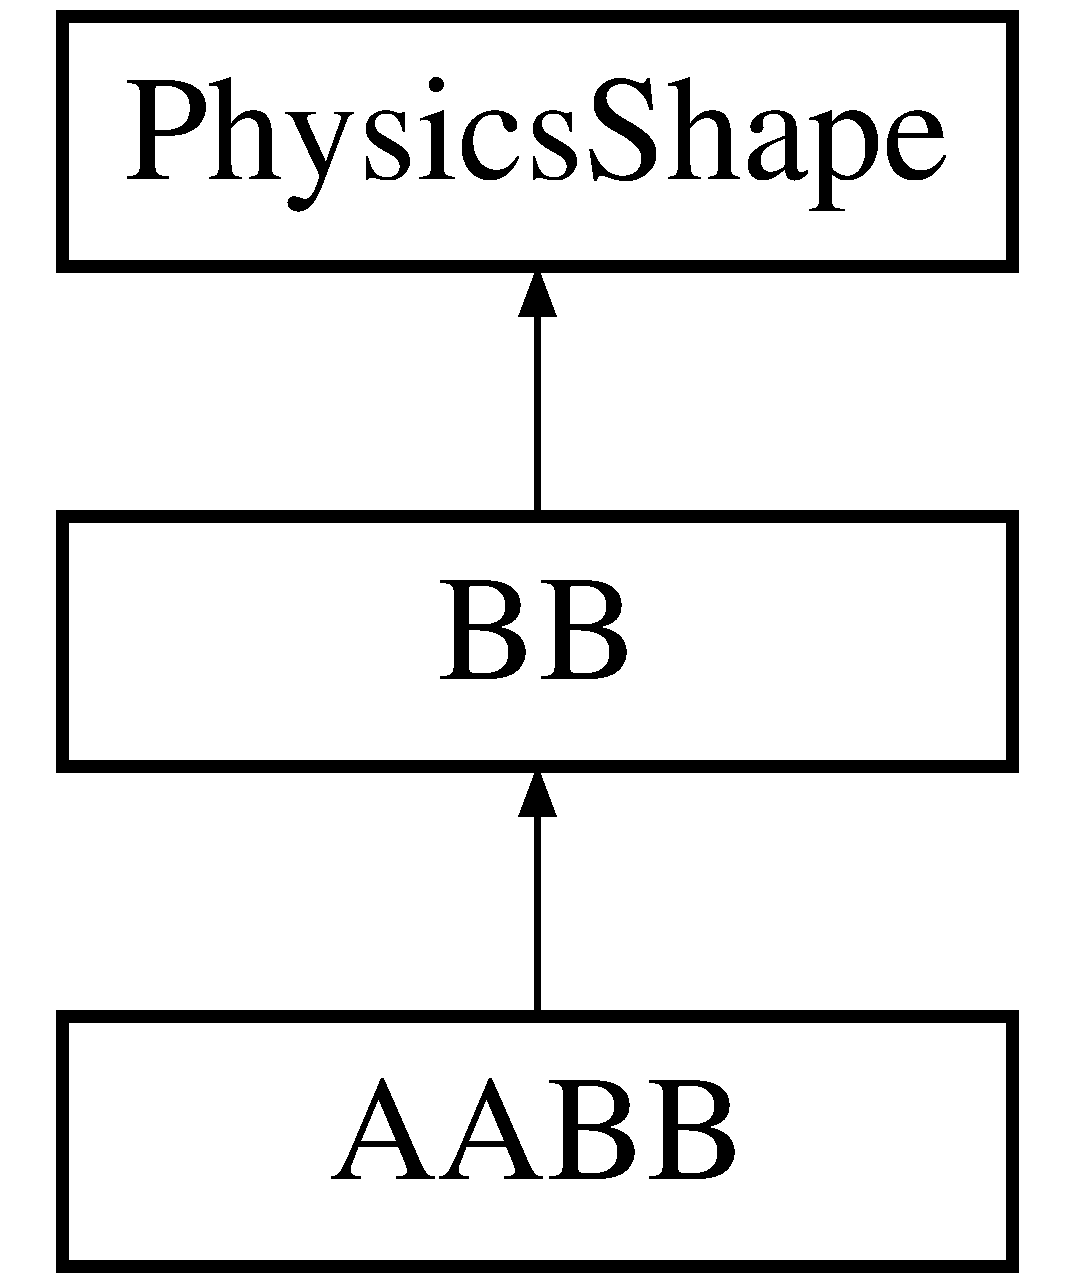
\includegraphics[height=3.000000cm]{class_a_a_b_b}
\end{center}
\end{figure}
\subsection*{Public Member Functions}
\begin{DoxyCompactItemize}
\item 
\hypertarget{class_a_a_b_b_a02dd4417acfbf243c183b98087305ef5}{\hyperlink{class_a_a_b_b_a02dd4417acfbf243c183b98087305ef5}{A\+A\+B\+B} (const \hyperlink{class_vector2_d}{Vector2\+D}$<$ float $>$ \&k\+Half)}\label{class_a_a_b_b_a02dd4417acfbf243c183b98087305ef5}

\begin{DoxyCompactList}\small\item\em Default Constructor. \end{DoxyCompactList}\item 
\hypertarget{class_a_a_b_b_aa3273dd7c64243f28cd2d11f7c4f5b8c}{virtual float \hyperlink{class_a_a_b_b_aa3273dd7c64243f28cd2d11f7c4f5b8c}{compute\+Inertia} (const float kf\+Mass) const }\label{class_a_a_b_b_aa3273dd7c64243f28cd2d11f7c4f5b8c}

\begin{DoxyCompactList}\small\item\em Constructor which takes Half Extents. \end{DoxyCompactList}\item 
\hypertarget{class_a_a_b_b_a14f5bf01839aacdc7f3317b326c83957}{virtual float \hyperlink{class_a_a_b_b_a14f5bf01839aacdc7f3317b326c83957}{compute\+Area} () const }\label{class_a_a_b_b_a14f5bf01839aacdc7f3317b326c83957}

\begin{DoxyCompactList}\small\item\em Compute the moment of inertia of the shape. \end{DoxyCompactList}\end{DoxyCompactItemize}
\subsection*{Additional Inherited Members}


\subsection{Detailed Description}
a non-\/\+Orientated Bounding \hyperlink{class_box}{Box} which inherits from \hyperlink{class_b_b}{B\+B} 

The documentation for this class was generated from the following file\+:\begin{DoxyCompactItemize}
\item 
include/\hyperlink{_b_b_8h}{B\+B.\+h}\end{DoxyCompactItemize}

\hypertarget{class_asteroid}{\section{Asteroid Class Reference}
\label{class_asteroid}\index{Asteroid@{Asteroid}}
}


an \hyperlink{class_asteroid}{Asteroid} with physics (inherits from the \hyperlink{class_physics_sprite}{Physics\+Sprite} class)  




{\ttfamily \#include $<$Asteroid.\+h$>$}

Inheritance diagram for Asteroid\+:\begin{figure}[H]
\begin{center}
\leavevmode
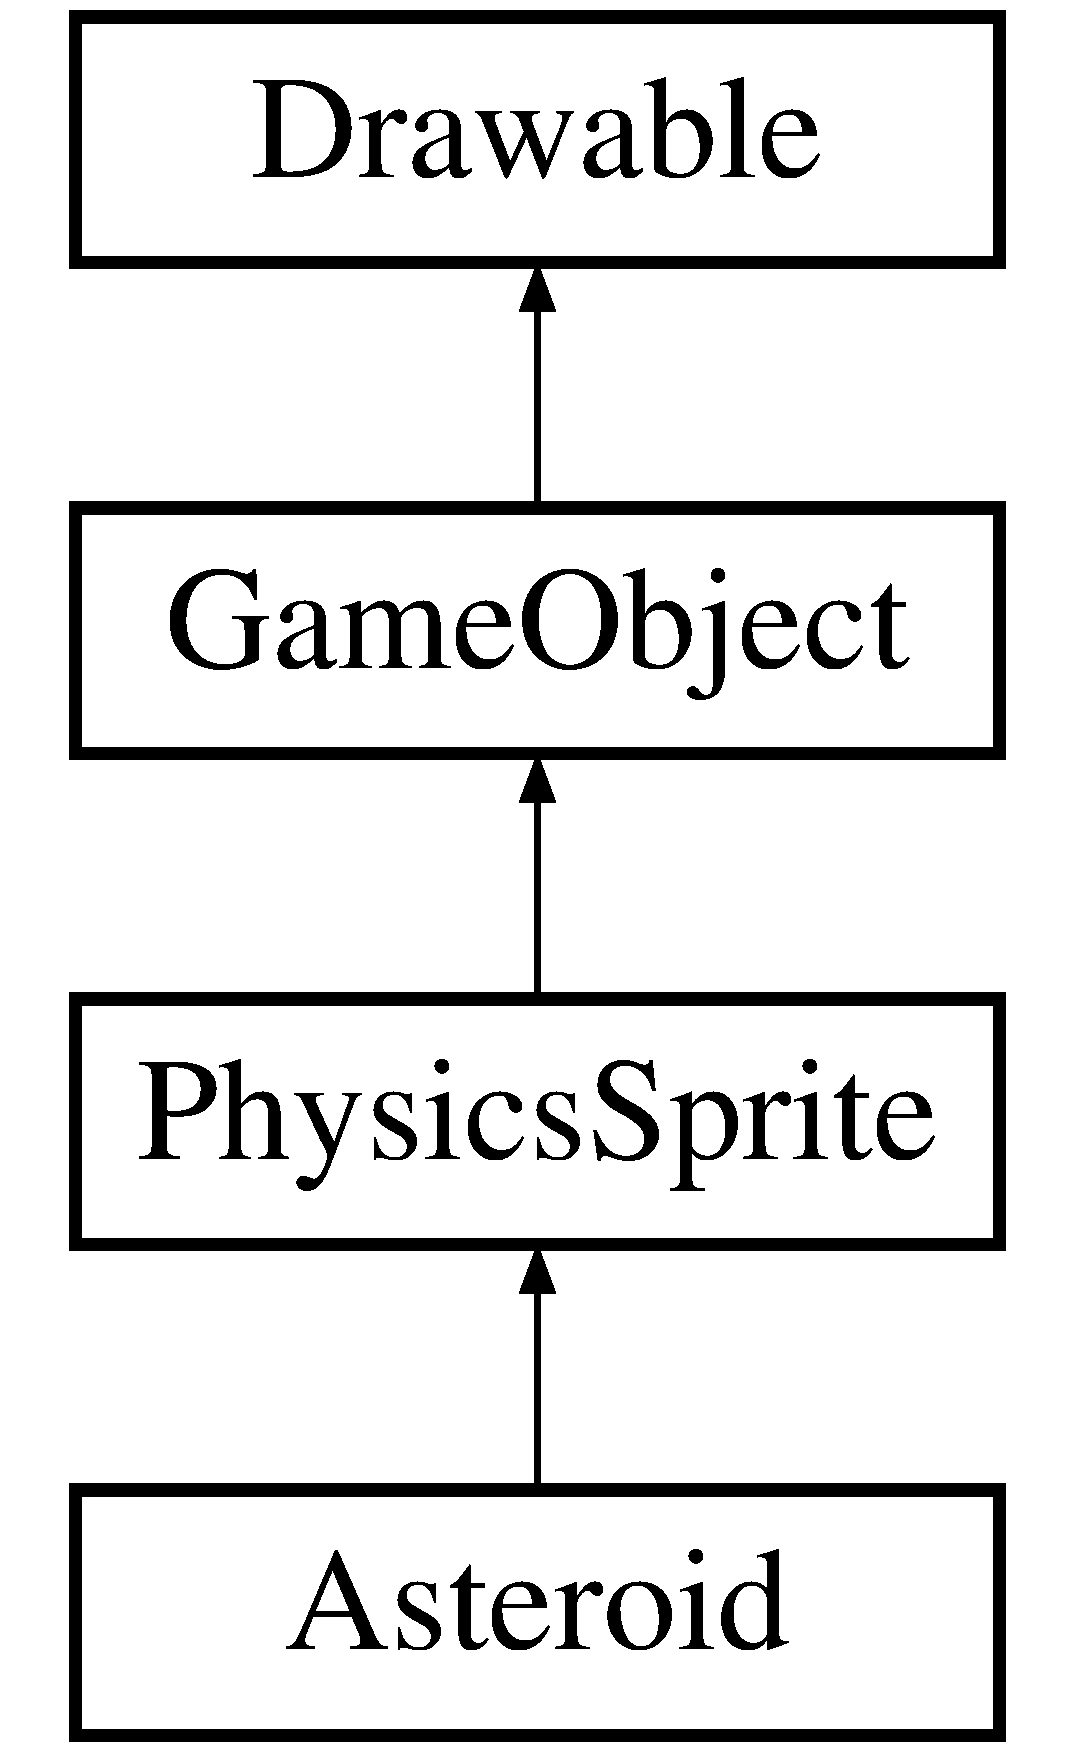
\includegraphics[height=4.000000cm]{class_asteroid}
\end{center}
\end{figure}
\subsection*{Public Member Functions}
\begin{DoxyCompactItemize}
\item 
\hypertarget{class_asteroid_a603c2eb87a4ed26c5b3fb06e953d611c}{\hyperlink{class_asteroid_a603c2eb87a4ed26c5b3fb06e953d611c}{Asteroid} ()}\label{class_asteroid_a603c2eb87a4ed26c5b3fb06e953d611c}

\begin{DoxyCompactList}\small\item\em Default Constructor. \end{DoxyCompactList}\item 
\hyperlink{class_asteroid_a395540293c8824104326aebeb4150e24}{Asteroid} (const \hyperlink{class_vector2_d}{Vector2\+D}$<$ float $>$ \&k\+Pos, const sf\+::\+Texture \&k\+Text)
\begin{DoxyCompactList}\small\item\em Constructor which takes a vector position and a texture. \end{DoxyCompactList}\end{DoxyCompactItemize}
\subsection*{Additional Inherited Members}


\subsection{Detailed Description}
an \hyperlink{class_asteroid}{Asteroid} with physics (inherits from the \hyperlink{class_physics_sprite}{Physics\+Sprite} class) 

\subsection{Constructor \& Destructor Documentation}
\hypertarget{class_asteroid_a395540293c8824104326aebeb4150e24}{\index{Asteroid@{Asteroid}!Asteroid@{Asteroid}}
\index{Asteroid@{Asteroid}!Asteroid@{Asteroid}}
\subsubsection[{Asteroid}]{\setlength{\rightskip}{0pt plus 5cm}Asteroid\+::\+Asteroid (
\begin{DoxyParamCaption}
\item[{const {\bf Vector2\+D}$<$ float $>$ \&}]{k\+Pos, }
\item[{const sf\+::\+Texture \&}]{k\+Text}
\end{DoxyParamCaption}
)}}\label{class_asteroid_a395540293c8824104326aebeb4150e24}


Constructor which takes a vector position and a texture. 


\begin{DoxyParams}{Parameters}
{\em k\+Pos} & Poisition \\
\hline
{\em k\+Text} & Texture \\
\hline
\end{DoxyParams}


The documentation for this class was generated from the following files\+:\begin{DoxyCompactItemize}
\item 
include/\hyperlink{_asteroid_8h}{Asteroid.\+h}\item 
src/\hyperlink{_asteroid_8cpp}{Asteroid.\+cpp}\end{DoxyCompactItemize}

\hypertarget{class_asteroid_field}{\section{Asteroid\+Field Class Reference}
\label{class_asteroid_field}\index{Asteroid\+Field@{Asteroid\+Field}}
}


a drawable which overlays on the screen when the gamee is paused or the game is over  




{\ttfamily \#include $<$Asteroid\+Field.\+h$>$}

Inheritance diagram for Asteroid\+Field\+:\begin{figure}[H]
\begin{center}
\leavevmode
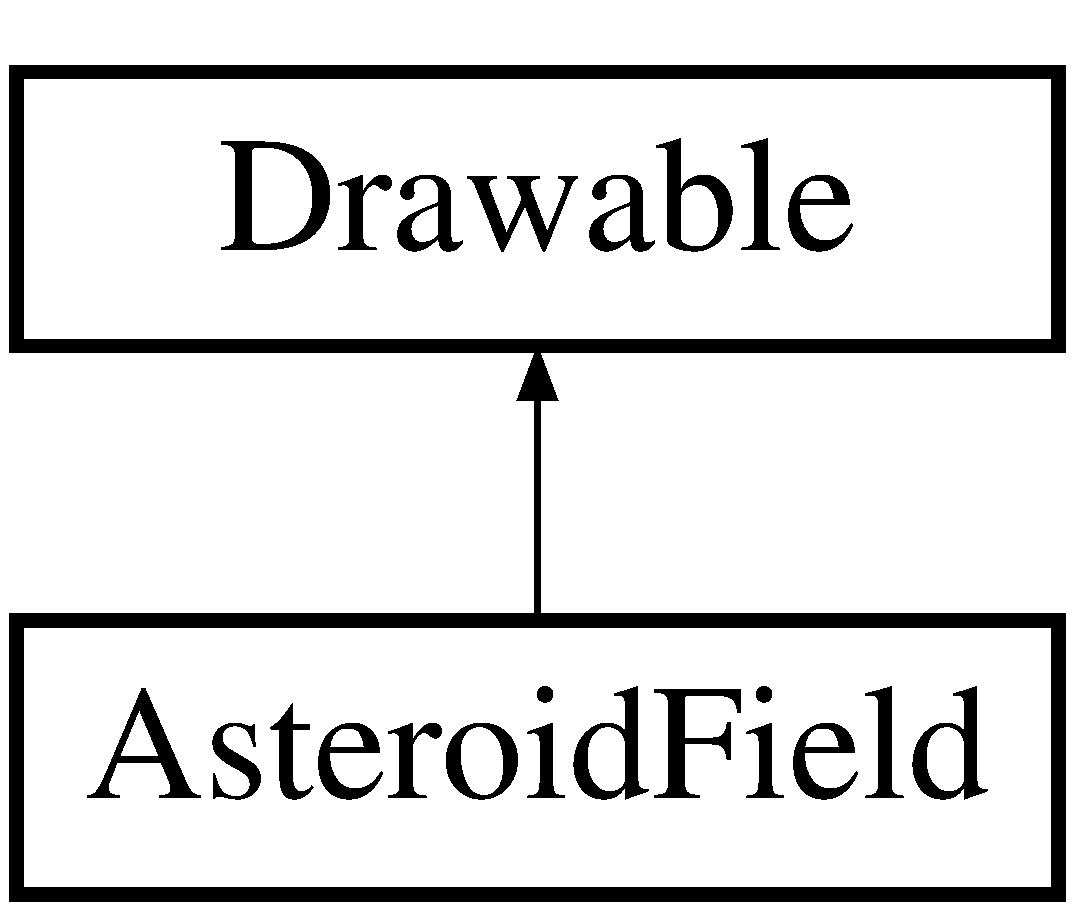
\includegraphics[height=2.000000cm]{class_asteroid_field}
\end{center}
\end{figure}
\subsection*{Public Member Functions}
\begin{DoxyCompactItemize}
\item 
\hypertarget{class_asteroid_field_a9daa07f82c9db387fa3612bed2c838a1}{\hyperlink{class_asteroid_field_a9daa07f82c9db387fa3612bed2c838a1}{Asteroid\+Field} ()}\label{class_asteroid_field_a9daa07f82c9db387fa3612bed2c838a1}

\begin{DoxyCompactList}\small\item\em Default constructor. \end{DoxyCompactList}\item 
\hyperlink{class_asteroid_field_aabdc29f8581421b92fb498d2b2a1d879}{Asteroid\+Field} (const \hyperlink{class_vector2_d}{Vector2\+D}$<$ float $>$ \&k\+Pos, const unsigned int kui\+Number\+Of\+Asteroids, const \hyperlink{class_vector2_d}{Vector2\+D}$<$ int $>$ \&k\+Size, const sf\+::\+Texture \&k\+Text)
\begin{DoxyCompactList}\small\item\em Constructor which takes a position, number of asteroids, size of the asteroid field and a texture. \end{DoxyCompactList}\item 
virtual void \hyperlink{class_asteroid_field_a4ba084eea3b8664c6b4fc6de61c9bc63}{draw} (sf\+::\+Render\+Target \&target, sf\+::\+Render\+States states) const 
\begin{DoxyCompactList}\small\item\em Draw the asteroid field. \end{DoxyCompactList}\end{DoxyCompactItemize}
\subsection*{Public Attributes}
\begin{DoxyCompactItemize}
\item 
\hypertarget{class_asteroid_field_a91d936bf0a4f0ffce8caa3d310ae04b0}{std\+::vector$<$ std\+::shared\+\_\+ptr\\*
$<$ \hyperlink{class_asteroid}{Asteroid} $>$ $>$ \hyperlink{class_asteroid_field_a91d936bf0a4f0ffce8caa3d310ae04b0}{g\+\_\+p\+Asteroids}}\label{class_asteroid_field_a91d936bf0a4f0ffce8caa3d310ae04b0}

\begin{DoxyCompactList}\small\item\em Vector of pointers to asteroids. \end{DoxyCompactList}\end{DoxyCompactItemize}


\subsection{Detailed Description}
a drawable which overlays on the screen when the gamee is paused or the game is over 

\subsection{Constructor \& Destructor Documentation}
\hypertarget{class_asteroid_field_aabdc29f8581421b92fb498d2b2a1d879}{\index{Asteroid\+Field@{Asteroid\+Field}!Asteroid\+Field@{Asteroid\+Field}}
\index{Asteroid\+Field@{Asteroid\+Field}!Asteroid\+Field@{Asteroid\+Field}}
\subsubsection[{Asteroid\+Field}]{\setlength{\rightskip}{0pt plus 5cm}Asteroid\+Field\+::\+Asteroid\+Field (
\begin{DoxyParamCaption}
\item[{const {\bf Vector2\+D}$<$ float $>$ \&}]{k\+Pos, }
\item[{const unsigned int}]{kui\+Number\+Of\+Asteroids, }
\item[{const {\bf Vector2\+D}$<$ int $>$ \&}]{k\+Size, }
\item[{const sf\+::\+Texture \&}]{k\+Text}
\end{DoxyParamCaption}
)}}\label{class_asteroid_field_aabdc29f8581421b92fb498d2b2a1d879}


Constructor which takes a position, number of asteroids, size of the asteroid field and a texture. 


\begin{DoxyParams}{Parameters}
{\em k\+Pos} & Position value \\
\hline
{\em kui\+Number\+Of\+Asteroids} & Number of asteroids in the field \\
\hline
{\em k\+Text} & Constructor which takes a position, number of asteroids, size of the asteroid field and a texture \\
\hline
\end{DoxyParams}


\subsection{Member Function Documentation}
\hypertarget{class_asteroid_field_a4ba084eea3b8664c6b4fc6de61c9bc63}{\index{Asteroid\+Field@{Asteroid\+Field}!draw@{draw}}
\index{draw@{draw}!Asteroid\+Field@{Asteroid\+Field}}
\subsubsection[{draw}]{\setlength{\rightskip}{0pt plus 5cm}void Asteroid\+Field\+::draw (
\begin{DoxyParamCaption}
\item[{sf\+::\+Render\+Target \&}]{target, }
\item[{sf\+::\+Render\+States}]{states}
\end{DoxyParamCaption}
) const\hspace{0.3cm}{\ttfamily [virtual]}}}\label{class_asteroid_field_a4ba084eea3b8664c6b4fc6de61c9bc63}


Draw the asteroid field. 

$<$ Draw the asteroid field 

The documentation for this class was generated from the following files\+:\begin{DoxyCompactItemize}
\item 
include/\hyperlink{_asteroid_field_8h}{Asteroid\+Field.\+h}\item 
src/\hyperlink{_asteroid_field_8cpp}{Asteroid\+Field.\+cpp}\end{DoxyCompactItemize}

\hypertarget{class_ball}{\section{Ball Class Reference}
\label{class_ball}\index{Ball@{Ball}}
}


A ball with a sprite physics.  




{\ttfamily \#include $<$Ball.\+h$>$}

Inheritance diagram for Ball\+:\begin{figure}[H]
\begin{center}
\leavevmode
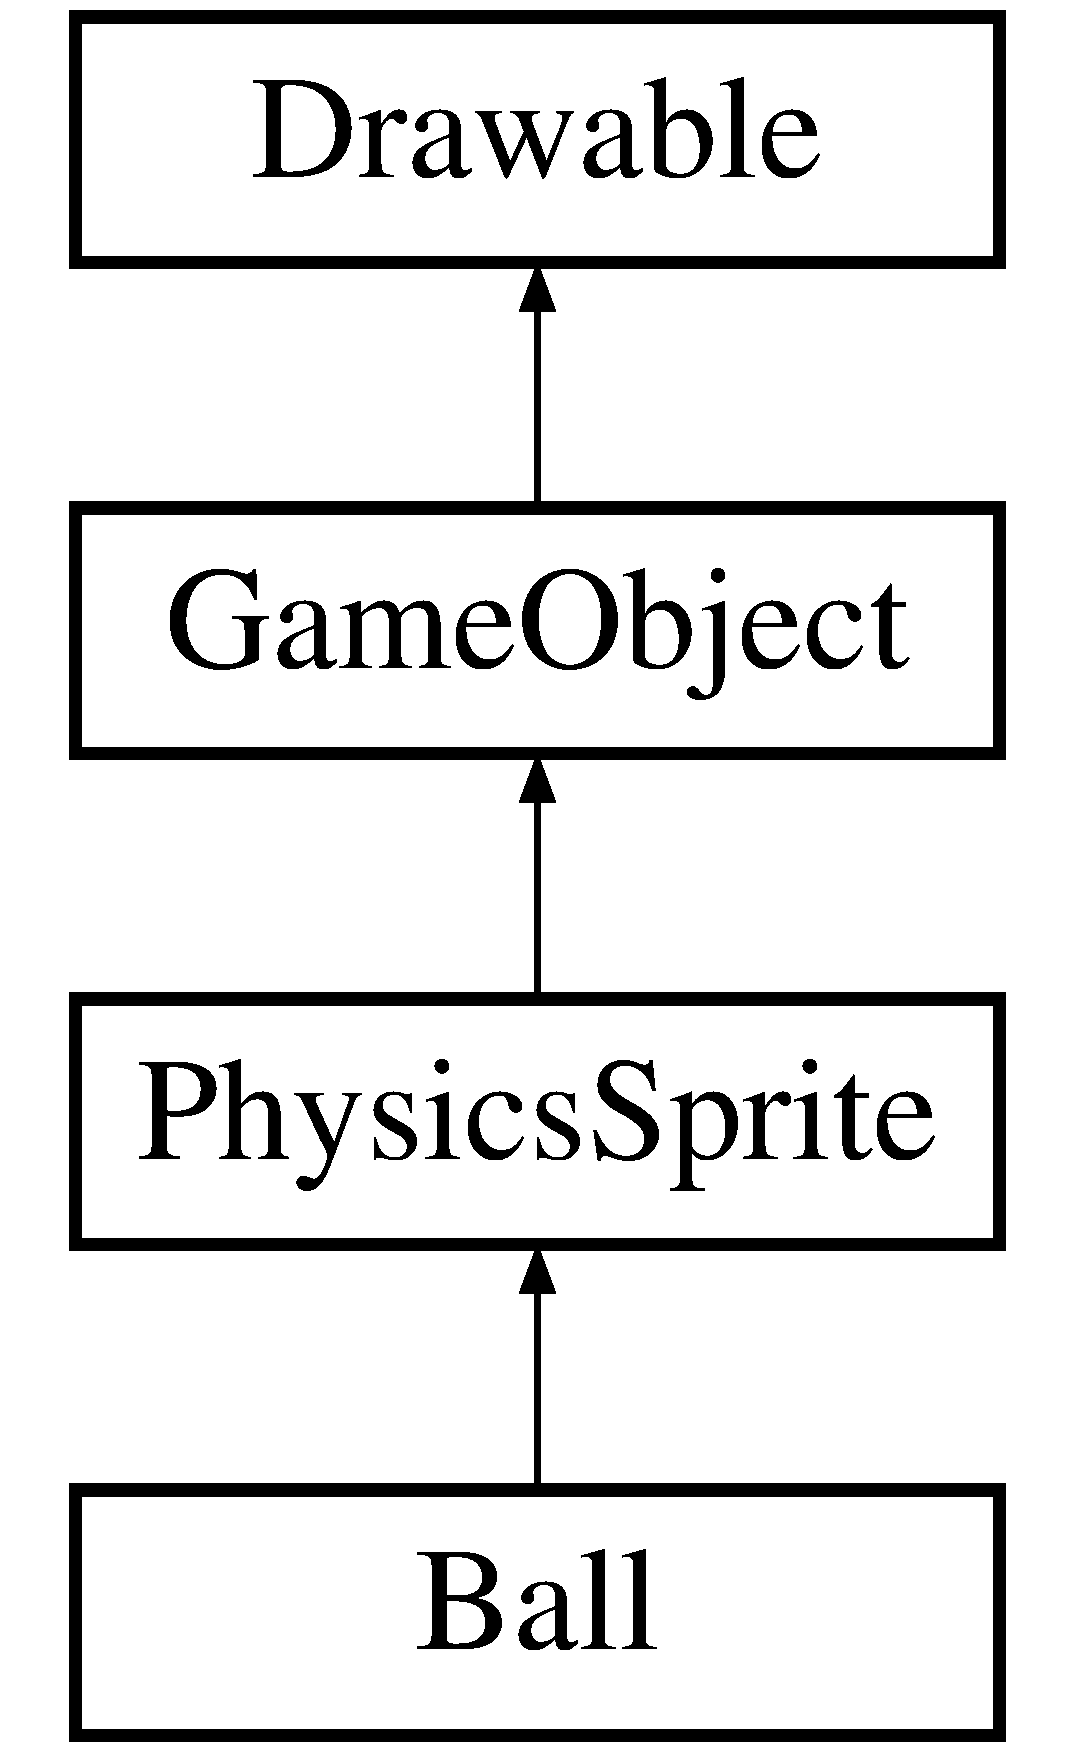
\includegraphics[height=4.000000cm]{class_ball}
\end{center}
\end{figure}
\subsection*{Public Member Functions}
\begin{DoxyCompactItemize}
\item 
\hypertarget{class_ball_a86a144d3dad6c953e422e32435923bbb}{\hyperlink{class_ball_a86a144d3dad6c953e422e32435923bbb}{Ball} ()}\label{class_ball_a86a144d3dad6c953e422e32435923bbb}

\begin{DoxyCompactList}\small\item\em Default contructor. \end{DoxyCompactList}\item 
\hyperlink{class_ball_a201d0014f0c644d3d3db54423925dd98}{Ball} (const \hyperlink{class_vector2_d}{Vector2\+D}$<$ float $>$ \&k\+Pos, const \hyperlink{class_vector2_d}{Vector2\+D}$<$ float $>$ \&k\+Vel, const sf\+::\+Texture \&k\+Text)
\begin{DoxyCompactList}\small\item\em Constructor which takes position, velocity and acceleration. \end{DoxyCompactList}\end{DoxyCompactItemize}
\subsection*{Public Attributes}
\begin{DoxyCompactItemize}
\item 
\hypertarget{class_ball_a66614ed7075be75dbe59a442779e8994}{std\+::shared\+\_\+ptr$<$ \hyperlink{class_c_c}{C\+C} $>$ \hyperlink{class_ball_a66614ed7075be75dbe59a442779e8994}{g\+\_\+p\+Phys\+Shape}}\label{class_ball_a66614ed7075be75dbe59a442779e8994}

\begin{DoxyCompactList}\small\item\em Circle physics body of the particle. \end{DoxyCompactList}\end{DoxyCompactItemize}
\subsection*{Additional Inherited Members}


\subsection{Detailed Description}
A ball with a sprite physics. 

\subsection{Constructor \& Destructor Documentation}
\hypertarget{class_ball_a201d0014f0c644d3d3db54423925dd98}{\index{Ball@{Ball}!Ball@{Ball}}
\index{Ball@{Ball}!Ball@{Ball}}
\subsubsection[{Ball}]{\setlength{\rightskip}{0pt plus 5cm}Ball\+::\+Ball (
\begin{DoxyParamCaption}
\item[{const {\bf Vector2\+D}$<$ float $>$ \&}]{k\+Pos, }
\item[{const {\bf Vector2\+D}$<$ float $>$ \&}]{k\+Vel, }
\item[{const sf\+::\+Texture \&}]{k\+Text}
\end{DoxyParamCaption}
)}}\label{class_ball_a201d0014f0c644d3d3db54423925dd98}


Constructor which takes position, velocity and acceleration. 


\begin{DoxyParams}{Parameters}
{\em k\+Pos} & initial position \\
\hline
{\em k\+Vel} & initial velocity \\
\hline
{\em k\+Text} & Constructor which takes position and velocity \\
\hline
\end{DoxyParams}


The documentation for this class was generated from the following files\+:\begin{DoxyCompactItemize}
\item 
include/\hyperlink{_ball_8h}{Ball.\+h}\item 
src/\hyperlink{_ball_8cpp}{Ball.\+cpp}\end{DoxyCompactItemize}

\hypertarget{class_b_b}{\section{B\+B Class Reference}
\label{class_b_b}\index{B\+B@{B\+B}}
}


a Bounding \hyperlink{class_box}{Box} which inherits from \hyperlink{class_physics_shape}{Physics\+Shape}  




{\ttfamily \#include $<$B\+B.\+h$>$}

Inheritance diagram for B\+B\+:\begin{figure}[H]
\begin{center}
\leavevmode
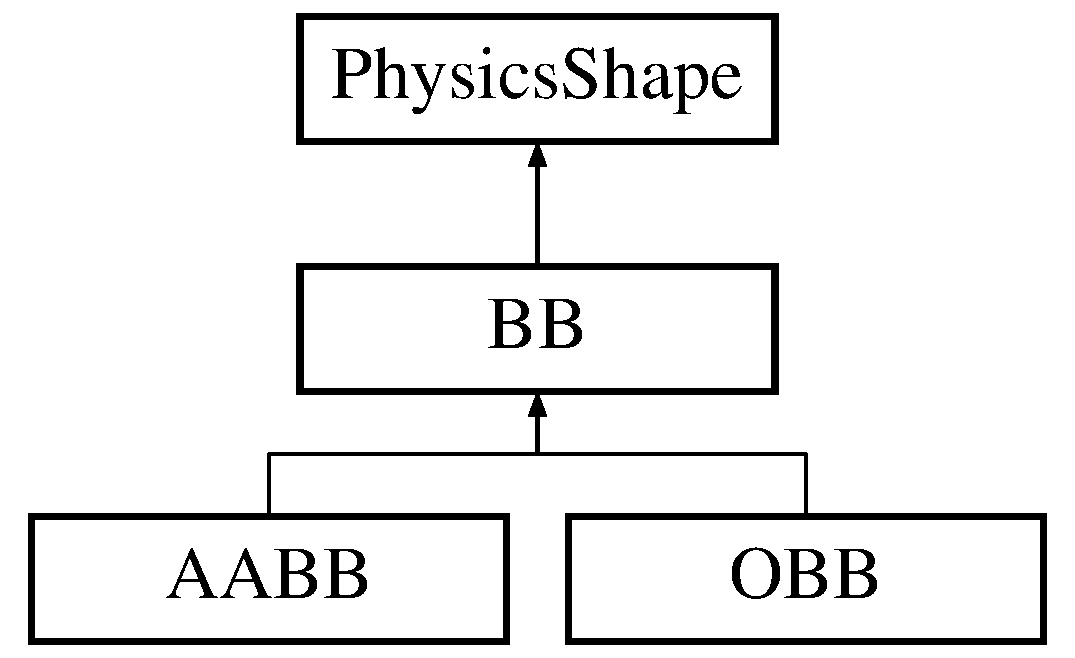
\includegraphics[height=3.000000cm]{class_b_b}
\end{center}
\end{figure}
\subsection*{Public Member Functions}
\begin{DoxyCompactItemize}
\item 
\hypertarget{class_b_b_ab2ee40c3f06e1ff92bbcfed63b571565}{\hyperlink{class_b_b_ab2ee40c3f06e1ff92bbcfed63b571565}{B\+B} (const \hyperlink{class_vector2_d}{Vector2\+D}$<$ float $>$ \&k\+Half)}\label{class_b_b_ab2ee40c3f06e1ff92bbcfed63b571565}

\begin{DoxyCompactList}\small\item\em Default Constructor. \end{DoxyCompactList}\item 
\hypertarget{class_b_b_ac3c2f415b7e81f0a04926738a6c40081}{void \hyperlink{class_b_b_ac3c2f415b7e81f0a04926738a6c40081}{set\+Half\+Extents} (const \hyperlink{class_vector2_d}{Vector2\+D}$<$ float $>$ \&k\+Half\+Vec)}\label{class_b_b_ac3c2f415b7e81f0a04926738a6c40081}

\begin{DoxyCompactList}\small\item\em Constructor which takes Half Extents. \end{DoxyCompactList}\item 
\hypertarget{class_b_b_a77e5f3c60978b35a4c5c5daa9185dcbf}{\hyperlink{class_vector2_d}{Vector2\+D}$<$ float $>$ \hyperlink{class_b_b_a77e5f3c60978b35a4c5c5daa9185dcbf}{get\+Half\+Extents} () const }\label{class_b_b_a77e5f3c60978b35a4c5c5daa9185dcbf}

\begin{DoxyCompactList}\small\item\em Sets the half extents. \end{DoxyCompactList}\item 
\hypertarget{class_b_b_ae015b360c554243f6024e0939e9a7760}{\hyperlink{class_vector2_d}{Vector2\+D}$<$ float $>$ \hyperlink{class_b_b_ae015b360c554243f6024e0939e9a7760}{get\+Min} () const }\label{class_b_b_ae015b360c554243f6024e0939e9a7760}

\begin{DoxyCompactList}\small\item\em Returns the half extents. \end{DoxyCompactList}\item 
\hypertarget{class_b_b_a4e4856d6d91a5c0995cefcf6157dcf2f}{\hyperlink{class_vector2_d}{Vector2\+D}$<$ float $>$ \hyperlink{class_b_b_a4e4856d6d91a5c0995cefcf6157dcf2f}{get\+Max} () const }\label{class_b_b_a4e4856d6d91a5c0995cefcf6157dcf2f}

\begin{DoxyCompactList}\small\item\em Gets the minimum of the extents. \end{DoxyCompactList}\end{DoxyCompactItemize}
\subsection*{Protected Attributes}
\begin{DoxyCompactItemize}
\item 
\hypertarget{class_b_b_ac9d77e6dad4861600b9a40fe160e7f83}{\hyperlink{class_vector2_d}{Vector2\+D}$<$ float $>$ \hyperlink{class_b_b_ac9d77e6dad4861600b9a40fe160e7f83}{m\+\_\+half\+Extents}}\label{class_b_b_ac9d77e6dad4861600b9a40fe160e7f83}

\begin{DoxyCompactList}\small\item\em Half Extents of the box. \end{DoxyCompactList}\end{DoxyCompactItemize}


\subsection{Detailed Description}
a Bounding \hyperlink{class_box}{Box} which inherits from \hyperlink{class_physics_shape}{Physics\+Shape} 

The documentation for this class was generated from the following file\+:\begin{DoxyCompactItemize}
\item 
include/\hyperlink{_b_b_8h}{B\+B.\+h}\end{DoxyCompactItemize}

\hypertarget{class_body2_d}{\section{Body2\+D Class Reference}
\label{class_body2_d}\index{Body2\+D@{Body2\+D}}
}


A 2\+D physics body.  




{\ttfamily \#include $<$Body2\+D.\+h$>$}

Inheritance diagram for Body2\+D\+:\begin{figure}[H]
\begin{center}
\leavevmode
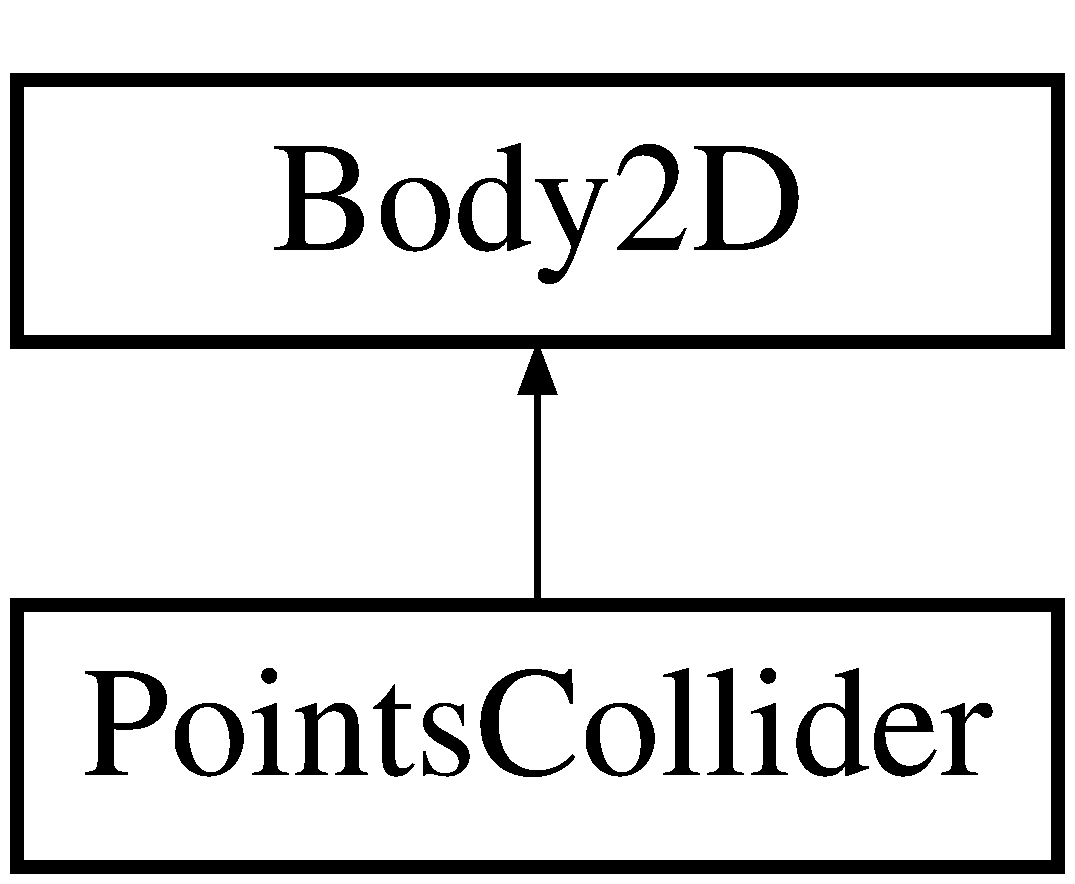
\includegraphics[height=2.000000cm]{class_body2_d}
\end{center}
\end{figure}
\subsection*{Public Member Functions}
\begin{DoxyCompactItemize}
\item 
\hypertarget{class_body2_d_a41ad3e71b95dfc818b91a19ae091b5d9}{\hyperlink{class_body2_d_a41ad3e71b95dfc818b91a19ae091b5d9}{Body2\+D} ()}\label{class_body2_d_a41ad3e71b95dfc818b91a19ae091b5d9}

\begin{DoxyCompactList}\small\item\em Default Constructor. \end{DoxyCompactList}\item 
\hyperlink{class_body2_d_add81f8b764cd0903ad01685edf56665e}{Body2\+D} (std\+::shared\+\_\+ptr$<$ \hyperlink{class_physics_shape}{Physics\+Shape} $>$ p\+Shape)
\begin{DoxyCompactList}\small\item\em Constructor which takes physics shape pointer. \end{DoxyCompactList}\item 
\hyperlink{class_body2_d_a0ea7045a305603b7cd38dfc5f611ebc9}{Body2\+D} (std\+::shared\+\_\+ptr$<$ \hyperlink{class_physics_shape}{Physics\+Shape} $>$ p\+Shape, const float kf\+X, const float kf\+Y)
\begin{DoxyCompactList}\small\item\em Constructor which takes physics shape pointer and position for X and Y. \end{DoxyCompactList}\item 
\hyperlink{class_body2_d_a30838f1b90c3273d8c75ed815eaacb53}{Body2\+D} (std\+::shared\+\_\+ptr$<$ \hyperlink{class_physics_shape}{Physics\+Shape} $>$ p\+Shape, const \hyperlink{class_vector2_d}{Vector2\+D}$<$ float $>$ \&k\+Pos)
\begin{DoxyCompactList}\small\item\em Constructor which takes physics shape pointer and position vector. \end{DoxyCompactList}\item 
\hypertarget{class_body2_d_ade39c095deccf7df714b42f64af3c00e}{float {\bfseries get\+Mass} () const }\label{class_body2_d_ade39c095deccf7df714b42f64af3c00e}

\item 
\hypertarget{class_body2_d_a5c24fc01e7288f03b1b64b254a752cb8}{float \hyperlink{class_body2_d_a5c24fc01e7288f03b1b64b254a752cb8}{get\+Attractive\+Value} () const }\label{class_body2_d_a5c24fc01e7288f03b1b64b254a752cb8}

\begin{DoxyCompactList}\small\item\em Returns the mass of the object. \end{DoxyCompactList}\item 
\hypertarget{class_body2_d_a186299396d4997908742dded5d038d08}{float \hyperlink{class_body2_d_a186299396d4997908742dded5d038d08}{get\+Inv\+Mass} () const }\label{class_body2_d_a186299396d4997908742dded5d038d08}

\begin{DoxyCompactList}\small\item\em Returns the attractive value of the body. \end{DoxyCompactList}\item 
\hypertarget{class_body2_d_acc065c0b756382f13e60007b3fb744cc}{float \hyperlink{class_body2_d_acc065c0b756382f13e60007b3fb744cc}{get\+Restitution} () const }\label{class_body2_d_acc065c0b756382f13e60007b3fb744cc}

\begin{DoxyCompactList}\small\item\em Returns the inverse mass of the body. \end{DoxyCompactList}\item 
\hypertarget{class_body2_d_a5a134ecd508bf33e21e29daf6bef9752}{float \hyperlink{class_body2_d_a5a134ecd508bf33e21e29daf6bef9752}{get\+Friction} () const }\label{class_body2_d_a5a134ecd508bf33e21e29daf6bef9752}

\begin{DoxyCompactList}\small\item\em Returns the restitution of the body. \end{DoxyCompactList}\item 
\hypertarget{class_body2_d_a26811630bb15275fd33548e20b5a65f2}{float \hyperlink{class_body2_d_a26811630bb15275fd33548e20b5a65f2}{get\+Density} () const }\label{class_body2_d_a26811630bb15275fd33548e20b5a65f2}

\begin{DoxyCompactList}\small\item\em Return the friction value of the body. \end{DoxyCompactList}\item 
\hypertarget{class_body2_d_a3ef473f845ad2d8cbbc38b8afbaa5737}{float \hyperlink{class_body2_d_a3ef473f845ad2d8cbbc38b8afbaa5737}{get\+Gravity\+Scale} () const }\label{class_body2_d_a3ef473f845ad2d8cbbc38b8afbaa5737}

\begin{DoxyCompactList}\small\item\em Returns the density of the body. \end{DoxyCompactList}\item 
\hypertarget{class_body2_d_ab9a9164631ae99f75a3934ecadc8a940}{float \hyperlink{class_body2_d_ab9a9164631ae99f75a3934ecadc8a940}{get\+Angular\+Velocity} () const }\label{class_body2_d_ab9a9164631ae99f75a3934ecadc8a940}

\begin{DoxyCompactList}\small\item\em Return the gravity scalar of the body. \end{DoxyCompactList}\item 
\hypertarget{class_body2_d_a8bbed510d49dc7f38ce35027af2e863b}{float \hyperlink{class_body2_d_a8bbed510d49dc7f38ce35027af2e863b}{get\+Angle\+Radians} () const }\label{class_body2_d_a8bbed510d49dc7f38ce35027af2e863b}

\begin{DoxyCompactList}\small\item\em Returns the angular velocity of the body. \end{DoxyCompactList}\item 
\hypertarget{class_body2_d_a36eaf32fc309efd4e94261eff5c6b888}{float \hyperlink{class_body2_d_a36eaf32fc309efd4e94261eff5c6b888}{get\+Angle\+Degrees} () const }\label{class_body2_d_a36eaf32fc309efd4e94261eff5c6b888}

\begin{DoxyCompactList}\small\item\em Returns the angle of the body in radians. \end{DoxyCompactList}\item 
\hypertarget{class_body2_d_ab533c98d0de3941202bf51b326cca07c}{float \hyperlink{class_body2_d_ab533c98d0de3941202bf51b326cca07c}{get\+Inv\+Inertia} () const }\label{class_body2_d_ab533c98d0de3941202bf51b326cca07c}

\begin{DoxyCompactList}\small\item\em Returns the angle of the body converted to degrees. \end{DoxyCompactList}\item 
\hypertarget{class_body2_d_a4aa31574a94a2f0662d9fc9466caf833}{bool \hyperlink{class_body2_d_a4aa31574a94a2f0662d9fc9466caf833}{get\+Is\+Static} () const }\label{class_body2_d_a4aa31574a94a2f0662d9fc9466caf833}

\begin{DoxyCompactList}\small\item\em Returns the inverse inertia of the body. \end{DoxyCompactList}\item 
\hypertarget{class_body2_d_aaa665f93d6c29015d30e79971a07bd9c}{bool \hyperlink{class_body2_d_aaa665f93d6c29015d30e79971a07bd9c}{get\+Is\+Collidable} () const }\label{class_body2_d_aaa665f93d6c29015d30e79971a07bd9c}

\begin{DoxyCompactList}\small\item\em Returns true if the body is static. \end{DoxyCompactList}\item 
\hypertarget{class_body2_d_adb3f90843f11e83d9e6f26c4616f5027}{\hyperlink{class_vector2_d}{Vector2\+D}$<$ float $>$ \hyperlink{class_body2_d_adb3f90843f11e83d9e6f26c4616f5027}{get\+Velocity} () const }\label{class_body2_d_adb3f90843f11e83d9e6f26c4616f5027}

\begin{DoxyCompactList}\small\item\em Returns true if the body is collidable. \end{DoxyCompactList}\item 
\hypertarget{class_body2_d_a60aa04d76d895a516e767ebcf448b8b3}{std\+::shared\+\_\+ptr$<$ \hyperlink{class_physics_shape}{Physics\+Shape} $>$ \hyperlink{class_body2_d_a60aa04d76d895a516e767ebcf448b8b3}{get\+Physics\+Shape} () const }\label{class_body2_d_a60aa04d76d895a516e767ebcf448b8b3}

\begin{DoxyCompactList}\small\item\em Returns the velocity of the body in meters per second. \end{DoxyCompactList}\item 
void \hyperlink{class_body2_d_aa15cf4fc66cbde8f72e48d95b84b0617}{set\+Physics\+Shape} (const std\+::shared\+\_\+ptr$<$ \hyperlink{class_physics_shape}{Physics\+Shape} $>$ kp\+New\+Shape)
\begin{DoxyCompactList}\small\item\em Returns a pointer to the physics shape. \end{DoxyCompactList}\item 
void \hyperlink{class_body2_d_ad3578491d07b2632e86b0c15eb398a92}{set\+Attractive\+Value} (const float f\+New\+Value)
\item 
void \hyperlink{class_body2_d_ae527f69a23d2e396d66044be6b36bc53}{set\+Velocity} (const \hyperlink{class_vector2_d}{Vector2\+D}$<$ float $>$ \&k\+New\+Vel)
\begin{DoxyCompactList}\small\item\em Sets the attrative value of the body. \end{DoxyCompactList}\item 
void \hyperlink{class_body2_d_a793004b49b70f1eddce4a38ad1335d7f}{set\+Friction} (const float kf\+New\+Friction)
\begin{DoxyCompactList}\small\item\em Sets the velocity of the body. \end{DoxyCompactList}\item 
void \hyperlink{class_body2_d_a3c277f1520ac8724bf73db4f20928c66}{set\+Restitution} (const float kf\+New\+Restitution)
\begin{DoxyCompactList}\small\item\em Sets the friction of the body. \end{DoxyCompactList}\item 
void \hyperlink{class_body2_d_ad7afbaa626aa98692227a806551ad62e}{set\+Gravity\+Scale} (const float kf\+Gravity)
\begin{DoxyCompactList}\small\item\em Sets the restituion of the body. \end{DoxyCompactList}\item 
\hypertarget{class_body2_d_a72e770d9b06aafd6c87c07b4b8fd3c88}{void \hyperlink{class_body2_d_a72e770d9b06aafd6c87c07b4b8fd3c88}{set\+Static\+Position} ()}\label{class_body2_d_a72e770d9b06aafd6c87c07b4b8fd3c88}

\begin{DoxyCompactList}\small\item\em Sets the gravity scale of the body. \end{DoxyCompactList}\item 
\hypertarget{class_body2_d_a2273e785cdd8ad462888dcedae504352}{void \hyperlink{class_body2_d_a2273e785cdd8ad462888dcedae504352}{set\+Static\+Rotation} ()}\label{class_body2_d_a2273e785cdd8ad462888dcedae504352}

\begin{DoxyCompactList}\small\item\em Sets the body to a static position. \end{DoxyCompactList}\item 
\hypertarget{class_body2_d_a860b912334bb0030928d127541fe1346}{void \hyperlink{class_body2_d_a860b912334bb0030928d127541fe1346}{set\+Collidable} ()}\label{class_body2_d_a860b912334bb0030928d127541fe1346}

\begin{DoxyCompactList}\small\item\em Sets the body to a static rotation. \end{DoxyCompactList}\item 
\hypertarget{class_body2_d_a3d8a3b351cc4bff945bf63855a59f3f7}{void \hyperlink{class_body2_d_a3d8a3b351cc4bff945bf63855a59f3f7}{set\+Non\+Collidable} ()}\label{class_body2_d_a3d8a3b351cc4bff945bf63855a59f3f7}

\begin{DoxyCompactList}\small\item\em Sets the body to be a collidable. \end{DoxyCompactList}\item 
\hypertarget{class_body2_d_a448afd0afe8ef2c165018623ba365bd8}{void \hyperlink{class_body2_d_a448afd0afe8ef2c165018623ba365bd8}{set\+Dynamic} ()}\label{class_body2_d_a448afd0afe8ef2c165018623ba365bd8}

\begin{DoxyCompactList}\small\item\em Sets the body to be a non collidable. \end{DoxyCompactList}\item 
void \hyperlink{class_body2_d_a3eecaf97eb846f7a22afd326426ef976}{set\+Static} ()
\begin{DoxyCompactList}\small\item\em Sets the body to dynamic. \end{DoxyCompactList}\item 
void \hyperlink{class_body2_d_a965fe7a6d920ffb1027dd691070cd842}{set\+Angle} (float f\+New\+Rad)
\begin{DoxyCompactList}\small\item\em Sets the angle of the body in radians. \end{DoxyCompactList}\item 
void \hyperlink{class_body2_d_a7d14597b4f11c8343841038d29629e86}{set\+Angle\+Deg} (const float kf\+New\+Deg)
\item 
void \hyperlink{class_body2_d_a61efab7842abf77c748683d658930e62}{add\+Angle} (const float kf\+Rads)
\begin{DoxyCompactList}\small\item\em Sets the angle of the body in degrees. \end{DoxyCompactList}\item 
void \hyperlink{class_body2_d_adb2bf5ca96811517418044e13cd0d054}{set\+Density} (const float kf\+Density)
\begin{DoxyCompactList}\small\item\em Sets the density of the body. \end{DoxyCompactList}\item 
void \hyperlink{class_body2_d_a55a924e33d60711a39888f92a10afbd1}{update} (const \hyperlink{class_vector2_d}{Vector2\+D}$<$ float $>$ \&k\+Gravity)
\begin{DoxyCompactList}\small\item\em Updates the body by the timestep passing the world gravity. \end{DoxyCompactList}\item 
void \hyperlink{class_body2_d_afe9db9c16d070f5154d0ebc16bf08f44}{apply\+Impulse} (const \hyperlink{class_vector2_d}{Vector2\+D}$<$ float $>$ \&k\+Impulse, const \hyperlink{class_vector2_d}{Vector2\+D}$<$ float $>$ \&k\+Contact)
\begin{DoxyCompactList}\small\item\em Applies an impulse to the body. \end{DoxyCompactList}\item 
void \hyperlink{class_body2_d_a87e9b9c0e07fe872cecc40c1afbf8480}{apply\+Positional\+Force} (const \hyperlink{class_vector2_d}{Vector2\+D}$<$ float $>$ \&k\+Force)
\item 
void \hyperlink{class_body2_d_a26336b3683b7cbda826bba54b8feca7d}{apply\+Rotational\+Force} (const float kf\+Force)
\begin{DoxyCompactList}\small\item\em Applies a force to the body. \end{DoxyCompactList}\item 
virtual void \hyperlink{class_body2_d_a55c37afe7eaa21a51cb309a2f52e0fcc}{collided} (const std\+::shared\+\_\+ptr$<$ \hyperlink{class_body2_d}{Body2\+D} $>$ \&kp\+Other)
\begin{DoxyCompactList}\small\item\em Applies a rotational force to the body. \end{DoxyCompactList}\end{DoxyCompactItemize}
\subsection*{Public Attributes}
\begin{DoxyCompactItemize}
\item 
\hypertarget{class_body2_d_a9bc86abec92a5f54009c44bddaaa5a72}{std\+::shared\+\_\+ptr$<$ \hyperlink{class_rotation_matrix}{Rotation\+Matrix} $>$ \hyperlink{class_body2_d_a9bc86abec92a5f54009c44bddaaa5a72}{g\+\_\+p\+Matrix}}\label{class_body2_d_a9bc86abec92a5f54009c44bddaaa5a72}

\begin{DoxyCompactList}\small\item\em Pointer to the rotation matrix for the body. \end{DoxyCompactList}\item 
\hypertarget{class_body2_d_a4ef190415b59cd68d0e4ce6cf7d1b70e}{\hyperlink{class_vector2_d}{Vector2\+D}$<$ float $>$ \hyperlink{class_body2_d_a4ef190415b59cd68d0e4ce6cf7d1b70e}{g\+\_\+\+Position}}\label{class_body2_d_a4ef190415b59cd68d0e4ce6cf7d1b70e}

\begin{DoxyCompactList}\small\item\em Position in Meters. \end{DoxyCompactList}\item 
\hypertarget{class_body2_d_aeaef63e80b0dab7c7e57e0c2fe8b4c2a}{unsigned int \hyperlink{class_body2_d_aeaef63e80b0dab7c7e57e0c2fe8b4c2a}{g\+\_\+ui\+Tag}}\label{class_body2_d_aeaef63e80b0dab7c7e57e0c2fe8b4c2a}

\begin{DoxyCompactList}\small\item\em Tag of the body. \end{DoxyCompactList}\end{DoxyCompactItemize}
\subsection*{Protected Member Functions}
\begin{DoxyCompactItemize}
\item 
void \hyperlink{class_body2_d_a4499cdddbd429b901c76fd6c49680173}{set\+Mass} (const float kf\+New\+Mass)
\begin{DoxyCompactList}\small\item\em Set the mass of the body. \end{DoxyCompactList}\item 
void \hyperlink{class_body2_d_a174198d6fb7bd33d68b73f30c18826ef}{set\+Interia} (const float kf\+New\+Inertia)
\begin{DoxyCompactList}\small\item\em Set the inertia of the body. \end{DoxyCompactList}\end{DoxyCompactItemize}
\subsection*{Protected Attributes}
\begin{DoxyCompactItemize}
\item 
\hypertarget{class_body2_d_a5de7be8b20e630cb3431e2e30f0a4445}{\hyperlink{struct_material}{Material} \hyperlink{class_body2_d_a5de7be8b20e630cb3431e2e30f0a4445}{m\+\_\+\+Material}}\label{class_body2_d_a5de7be8b20e630cb3431e2e30f0a4445}

\begin{DoxyCompactList}\small\item\em Physics material for body. \end{DoxyCompactList}\end{DoxyCompactItemize}


\subsection{Detailed Description}
A 2\+D physics body. 

\subsection{Constructor \& Destructor Documentation}
\hypertarget{class_body2_d_add81f8b764cd0903ad01685edf56665e}{\index{Body2\+D@{Body2\+D}!Body2\+D@{Body2\+D}}
\index{Body2\+D@{Body2\+D}!Body2\+D@{Body2\+D}}
\subsubsection[{Body2\+D}]{\setlength{\rightskip}{0pt plus 5cm}Body2\+D\+::\+Body2\+D (
\begin{DoxyParamCaption}
\item[{std\+::shared\+\_\+ptr$<$ {\bf Physics\+Shape} $>$}]{p\+Shape}
\end{DoxyParamCaption}
)}}\label{class_body2_d_add81f8b764cd0903ad01685edf56665e}


Constructor which takes physics shape pointer. 


\begin{DoxyParams}{Parameters}
{\em p\+Shape} & Physics shape pointer \\
\hline
\end{DoxyParams}
\hypertarget{class_body2_d_a0ea7045a305603b7cd38dfc5f611ebc9}{\index{Body2\+D@{Body2\+D}!Body2\+D@{Body2\+D}}
\index{Body2\+D@{Body2\+D}!Body2\+D@{Body2\+D}}
\subsubsection[{Body2\+D}]{\setlength{\rightskip}{0pt plus 5cm}Body2\+D\+::\+Body2\+D (
\begin{DoxyParamCaption}
\item[{std\+::shared\+\_\+ptr$<$ {\bf Physics\+Shape} $>$}]{p\+Shape, }
\item[{const float}]{kf\+X, }
\item[{const float}]{kf\+Y}
\end{DoxyParamCaption}
)}}\label{class_body2_d_a0ea7045a305603b7cd38dfc5f611ebc9}


Constructor which takes physics shape pointer and position for X and Y. 


\begin{DoxyParams}{Parameters}
{\em p\+Shape} & Physics shape pointer \\
\hline
{\em kf\+X} & X position value \\
\hline
{\em kf\+Y} & Y position value \\
\hline
\end{DoxyParams}
\hypertarget{class_body2_d_a30838f1b90c3273d8c75ed815eaacb53}{\index{Body2\+D@{Body2\+D}!Body2\+D@{Body2\+D}}
\index{Body2\+D@{Body2\+D}!Body2\+D@{Body2\+D}}
\subsubsection[{Body2\+D}]{\setlength{\rightskip}{0pt plus 5cm}Body2\+D\+::\+Body2\+D (
\begin{DoxyParamCaption}
\item[{std\+::shared\+\_\+ptr$<$ {\bf Physics\+Shape} $>$}]{p\+Shape, }
\item[{const {\bf Vector2\+D}$<$ float $>$ \&}]{k\+Pos}
\end{DoxyParamCaption}
)}}\label{class_body2_d_a30838f1b90c3273d8c75ed815eaacb53}


Constructor which takes physics shape pointer and position vector. 


\begin{DoxyParams}{Parameters}
{\em p\+Shape} & Physics shape pointer \\
\hline
{\em k\+Pos} & Position value \\
\hline
\end{DoxyParams}


\subsection{Member Function Documentation}
\hypertarget{class_body2_d_a61efab7842abf77c748683d658930e62}{\index{Body2\+D@{Body2\+D}!add\+Angle@{add\+Angle}}
\index{add\+Angle@{add\+Angle}!Body2\+D@{Body2\+D}}
\subsubsection[{add\+Angle}]{\setlength{\rightskip}{0pt plus 5cm}void Body2\+D\+::add\+Angle (
\begin{DoxyParamCaption}
\item[{const float}]{kf\+Rads}
\end{DoxyParamCaption}
)}}\label{class_body2_d_a61efab7842abf77c748683d658930e62}


Sets the angle of the body in degrees. 

Adds an angle to the body in radians 
\begin{DoxyParams}{Parameters}
{\em kf\+Rads} & Change in angle in radians \\
\hline
\end{DoxyParams}
\hypertarget{class_body2_d_afe9db9c16d070f5154d0ebc16bf08f44}{\index{Body2\+D@{Body2\+D}!apply\+Impulse@{apply\+Impulse}}
\index{apply\+Impulse@{apply\+Impulse}!Body2\+D@{Body2\+D}}
\subsubsection[{apply\+Impulse}]{\setlength{\rightskip}{0pt plus 5cm}void Body2\+D\+::apply\+Impulse (
\begin{DoxyParamCaption}
\item[{const {\bf Vector2\+D}$<$ float $>$ \&}]{k\+Impulse, }
\item[{const {\bf Vector2\+D}$<$ float $>$ \&}]{k\+Contact}
\end{DoxyParamCaption}
)}}\label{class_body2_d_afe9db9c16d070f5154d0ebc16bf08f44}


Applies an impulse to the body. 


\begin{DoxyParams}{Parameters}
{\em k\+Impulse} & Impulse Vector \\
\hline
{\em k\+Contact} & Point of contact \\
\hline
\end{DoxyParams}
\hypertarget{class_body2_d_a87e9b9c0e07fe872cecc40c1afbf8480}{\index{Body2\+D@{Body2\+D}!apply\+Positional\+Force@{apply\+Positional\+Force}}
\index{apply\+Positional\+Force@{apply\+Positional\+Force}!Body2\+D@{Body2\+D}}
\subsubsection[{apply\+Positional\+Force}]{\setlength{\rightskip}{0pt plus 5cm}void Body2\+D\+::apply\+Positional\+Force (
\begin{DoxyParamCaption}
\item[{const {\bf Vector2\+D}$<$ float $>$ \&}]{k\+Force}
\end{DoxyParamCaption}
)\hspace{0.3cm}{\ttfamily [inline]}}}\label{class_body2_d_a87e9b9c0e07fe872cecc40c1afbf8480}

\begin{DoxyParams}{Parameters}
{\em k\+Force} & Force vector \\
\hline
\end{DoxyParams}
\hypertarget{class_body2_d_a26336b3683b7cbda826bba54b8feca7d}{\index{Body2\+D@{Body2\+D}!apply\+Rotational\+Force@{apply\+Rotational\+Force}}
\index{apply\+Rotational\+Force@{apply\+Rotational\+Force}!Body2\+D@{Body2\+D}}
\subsubsection[{apply\+Rotational\+Force}]{\setlength{\rightskip}{0pt plus 5cm}void Body2\+D\+::apply\+Rotational\+Force (
\begin{DoxyParamCaption}
\item[{const float}]{kf\+Force}
\end{DoxyParamCaption}
)\hspace{0.3cm}{\ttfamily [inline]}}}\label{class_body2_d_a26336b3683b7cbda826bba54b8feca7d}


Applies a force to the body. 


\begin{DoxyParams}{Parameters}
{\em kf\+Force} & Rotational force \\
\hline
\end{DoxyParams}
\hypertarget{class_body2_d_a55c37afe7eaa21a51cb309a2f52e0fcc}{\index{Body2\+D@{Body2\+D}!collided@{collided}}
\index{collided@{collided}!Body2\+D@{Body2\+D}}
\subsubsection[{collided}]{\setlength{\rightskip}{0pt plus 5cm}virtual void Body2\+D\+::collided (
\begin{DoxyParamCaption}
\item[{const std\+::shared\+\_\+ptr$<$ {\bf Body2\+D} $>$ \&}]{kp\+Other}
\end{DoxyParamCaption}
)\hspace{0.3cm}{\ttfamily [inline]}, {\ttfamily [virtual]}}}\label{class_body2_d_a55c37afe7eaa21a51cb309a2f52e0fcc}


Applies a rotational force to the body. 


\begin{DoxyParams}{Parameters}
{\em kp\+Other} & Pointer to the body which it collided with \\
\hline
\end{DoxyParams}


Reimplemented in \hyperlink{class_points_collider_ad24d2f1ba11e34a52e9caef300239de6}{Points\+Collider}.

\hypertarget{class_body2_d_a965fe7a6d920ffb1027dd691070cd842}{\index{Body2\+D@{Body2\+D}!set\+Angle@{set\+Angle}}
\index{set\+Angle@{set\+Angle}!Body2\+D@{Body2\+D}}
\subsubsection[{set\+Angle}]{\setlength{\rightskip}{0pt plus 5cm}void Body2\+D\+::set\+Angle (
\begin{DoxyParamCaption}
\item[{float}]{f\+New\+Rad}
\end{DoxyParamCaption}
)}}\label{class_body2_d_a965fe7a6d920ffb1027dd691070cd842}


Sets the angle of the body in radians. 


\begin{DoxyParams}{Parameters}
{\em f\+New\+Rad} & New angle in radians \\
\hline
\end{DoxyParams}
\hypertarget{class_body2_d_a7d14597b4f11c8343841038d29629e86}{\index{Body2\+D@{Body2\+D}!set\+Angle\+Deg@{set\+Angle\+Deg}}
\index{set\+Angle\+Deg@{set\+Angle\+Deg}!Body2\+D@{Body2\+D}}
\subsubsection[{set\+Angle\+Deg}]{\setlength{\rightskip}{0pt plus 5cm}void Body2\+D\+::set\+Angle\+Deg (
\begin{DoxyParamCaption}
\item[{const float}]{kf\+New\+Deg}
\end{DoxyParamCaption}
)\hspace{0.3cm}{\ttfamily [inline]}}}\label{class_body2_d_a7d14597b4f11c8343841038d29629e86}

\begin{DoxyParams}{Parameters}
{\em kf\+New\+Deg} & New angle in degrees \\
\hline
\end{DoxyParams}
\hypertarget{class_body2_d_ad3578491d07b2632e86b0c15eb398a92}{\index{Body2\+D@{Body2\+D}!set\+Attractive\+Value@{set\+Attractive\+Value}}
\index{set\+Attractive\+Value@{set\+Attractive\+Value}!Body2\+D@{Body2\+D}}
\subsubsection[{set\+Attractive\+Value}]{\setlength{\rightskip}{0pt plus 5cm}void Body2\+D\+::set\+Attractive\+Value (
\begin{DoxyParamCaption}
\item[{const float}]{f\+New\+Value}
\end{DoxyParamCaption}
)\hspace{0.3cm}{\ttfamily [inline]}}}\label{class_body2_d_ad3578491d07b2632e86b0c15eb398a92}

\begin{DoxyParams}{Parameters}
{\em f\+New\+Value} & New attractive value \\
\hline
\end{DoxyParams}
\hypertarget{class_body2_d_adb2bf5ca96811517418044e13cd0d054}{\index{Body2\+D@{Body2\+D}!set\+Density@{set\+Density}}
\index{set\+Density@{set\+Density}!Body2\+D@{Body2\+D}}
\subsubsection[{set\+Density}]{\setlength{\rightskip}{0pt plus 5cm}void Body2\+D\+::set\+Density (
\begin{DoxyParamCaption}
\item[{const float}]{kf\+Density}
\end{DoxyParamCaption}
)}}\label{class_body2_d_adb2bf5ca96811517418044e13cd0d054}


Sets the density of the body. 


\begin{DoxyParams}{Parameters}
{\em kf\+Density} & New density value \\
\hline
\end{DoxyParams}
\hypertarget{class_body2_d_a793004b49b70f1eddce4a38ad1335d7f}{\index{Body2\+D@{Body2\+D}!set\+Friction@{set\+Friction}}
\index{set\+Friction@{set\+Friction}!Body2\+D@{Body2\+D}}
\subsubsection[{set\+Friction}]{\setlength{\rightskip}{0pt plus 5cm}void Body2\+D\+::set\+Friction (
\begin{DoxyParamCaption}
\item[{const float}]{kf\+New\+Friction}
\end{DoxyParamCaption}
)\hspace{0.3cm}{\ttfamily [inline]}}}\label{class_body2_d_a793004b49b70f1eddce4a38ad1335d7f}


Sets the velocity of the body. 


\begin{DoxyParams}{Parameters}
{\em kf\+New\+Friction} & New friction value \\
\hline
\end{DoxyParams}
\hypertarget{class_body2_d_ad7afbaa626aa98692227a806551ad62e}{\index{Body2\+D@{Body2\+D}!set\+Gravity\+Scale@{set\+Gravity\+Scale}}
\index{set\+Gravity\+Scale@{set\+Gravity\+Scale}!Body2\+D@{Body2\+D}}
\subsubsection[{set\+Gravity\+Scale}]{\setlength{\rightskip}{0pt plus 5cm}void Body2\+D\+::set\+Gravity\+Scale (
\begin{DoxyParamCaption}
\item[{const float}]{kf\+Gravity}
\end{DoxyParamCaption}
)\hspace{0.3cm}{\ttfamily [inline]}}}\label{class_body2_d_ad7afbaa626aa98692227a806551ad62e}


Sets the restituion of the body. 


\begin{DoxyParams}{Parameters}
{\em kf\+Gravity} & New gravity scalar \\
\hline
\end{DoxyParams}
\hypertarget{class_body2_d_a174198d6fb7bd33d68b73f30c18826ef}{\index{Body2\+D@{Body2\+D}!set\+Interia@{set\+Interia}}
\index{set\+Interia@{set\+Interia}!Body2\+D@{Body2\+D}}
\subsubsection[{set\+Interia}]{\setlength{\rightskip}{0pt plus 5cm}void Body2\+D\+::set\+Interia (
\begin{DoxyParamCaption}
\item[{const float}]{kf\+New\+Inertia}
\end{DoxyParamCaption}
)\hspace{0.3cm}{\ttfamily [protected]}}}\label{class_body2_d_a174198d6fb7bd33d68b73f30c18826ef}


Set the inertia of the body. 


\begin{DoxyParams}{Parameters}
{\em kf\+New\+Inertia} & New inertia value \\
\hline
\end{DoxyParams}
\hypertarget{class_body2_d_a4499cdddbd429b901c76fd6c49680173}{\index{Body2\+D@{Body2\+D}!set\+Mass@{set\+Mass}}
\index{set\+Mass@{set\+Mass}!Body2\+D@{Body2\+D}}
\subsubsection[{set\+Mass}]{\setlength{\rightskip}{0pt plus 5cm}void Body2\+D\+::set\+Mass (
\begin{DoxyParamCaption}
\item[{const float}]{kf\+New\+Mass}
\end{DoxyParamCaption}
)\hspace{0.3cm}{\ttfamily [protected]}}}\label{class_body2_d_a4499cdddbd429b901c76fd6c49680173}


Set the mass of the body. 


\begin{DoxyParams}{Parameters}
{\em kf\+New\+Mass} & New mass value \\
\hline
\end{DoxyParams}
\hypertarget{class_body2_d_aa15cf4fc66cbde8f72e48d95b84b0617}{\index{Body2\+D@{Body2\+D}!set\+Physics\+Shape@{set\+Physics\+Shape}}
\index{set\+Physics\+Shape@{set\+Physics\+Shape}!Body2\+D@{Body2\+D}}
\subsubsection[{set\+Physics\+Shape}]{\setlength{\rightskip}{0pt plus 5cm}void Body2\+D\+::set\+Physics\+Shape (
\begin{DoxyParamCaption}
\item[{const std\+::shared\+\_\+ptr$<$ {\bf Physics\+Shape} $>$}]{kp\+New\+Shape}
\end{DoxyParamCaption}
)}}\label{class_body2_d_aa15cf4fc66cbde8f72e48d95b84b0617}


Returns a pointer to the physics shape. 

Sets the physics shape 
\begin{DoxyParams}{Parameters}
{\em kp\+New\+Shape} & Pointer to new physics shape \\
\hline
\end{DoxyParams}
\hypertarget{class_body2_d_a3c277f1520ac8724bf73db4f20928c66}{\index{Body2\+D@{Body2\+D}!set\+Restitution@{set\+Restitution}}
\index{set\+Restitution@{set\+Restitution}!Body2\+D@{Body2\+D}}
\subsubsection[{set\+Restitution}]{\setlength{\rightskip}{0pt plus 5cm}void Body2\+D\+::set\+Restitution (
\begin{DoxyParamCaption}
\item[{const float}]{kf\+New\+Restitution}
\end{DoxyParamCaption}
)\hspace{0.3cm}{\ttfamily [inline]}}}\label{class_body2_d_a3c277f1520ac8724bf73db4f20928c66}


Sets the friction of the body. 


\begin{DoxyParams}{Parameters}
{\em kf\+New\+Restitution} & New restiution value \\
\hline
\end{DoxyParams}
\hypertarget{class_body2_d_a3eecaf97eb846f7a22afd326426ef976}{\index{Body2\+D@{Body2\+D}!set\+Static@{set\+Static}}
\index{set\+Static@{set\+Static}!Body2\+D@{Body2\+D}}
\subsubsection[{set\+Static}]{\setlength{\rightskip}{0pt plus 5cm}void Body2\+D\+::set\+Static (
\begin{DoxyParamCaption}
{}
\end{DoxyParamCaption}
)}}\label{class_body2_d_a3eecaf97eb846f7a22afd326426ef976}


Sets the body to dynamic. 

Sets the body to static \hypertarget{class_body2_d_ae527f69a23d2e396d66044be6b36bc53}{\index{Body2\+D@{Body2\+D}!set\+Velocity@{set\+Velocity}}
\index{set\+Velocity@{set\+Velocity}!Body2\+D@{Body2\+D}}
\subsubsection[{set\+Velocity}]{\setlength{\rightskip}{0pt plus 5cm}void Body2\+D\+::set\+Velocity (
\begin{DoxyParamCaption}
\item[{const {\bf Vector2\+D}$<$ float $>$ \&}]{k\+New\+Vel}
\end{DoxyParamCaption}
)\hspace{0.3cm}{\ttfamily [inline]}}}\label{class_body2_d_ae527f69a23d2e396d66044be6b36bc53}


Sets the attrative value of the body. 


\begin{DoxyParams}{Parameters}
{\em k\+New\+Vel} & new velocity \\
\hline
\end{DoxyParams}
\hypertarget{class_body2_d_a55a924e33d60711a39888f92a10afbd1}{\index{Body2\+D@{Body2\+D}!update@{update}}
\index{update@{update}!Body2\+D@{Body2\+D}}
\subsubsection[{update}]{\setlength{\rightskip}{0pt plus 5cm}void Body2\+D\+::update (
\begin{DoxyParamCaption}
\item[{const {\bf Vector2\+D}$<$ float $>$ \&}]{k\+Gravity}
\end{DoxyParamCaption}
)}}\label{class_body2_d_a55a924e33d60711a39888f92a10afbd1}


Updates the body by the timestep passing the world gravity. 


\begin{DoxyParams}{Parameters}
{\em k\+Gravity} & Gravity value \\
\hline
\end{DoxyParams}


The documentation for this class was generated from the following files\+:\begin{DoxyCompactItemize}
\item 
include/\hyperlink{_body2_d_8h}{Body2\+D.\+h}\item 
src/\hyperlink{body2_d_8cpp}{body2\+D.\+cpp}\end{DoxyCompactItemize}

\hypertarget{class_box}{\section{Box Class Reference}
\label{class_box}\index{Box@{Box}}
}


a non orientated physics body with a solid colour  




{\ttfamily \#include $<$Box.\+h$>$}

Inheritance diagram for Box\+:\begin{figure}[H]
\begin{center}
\leavevmode
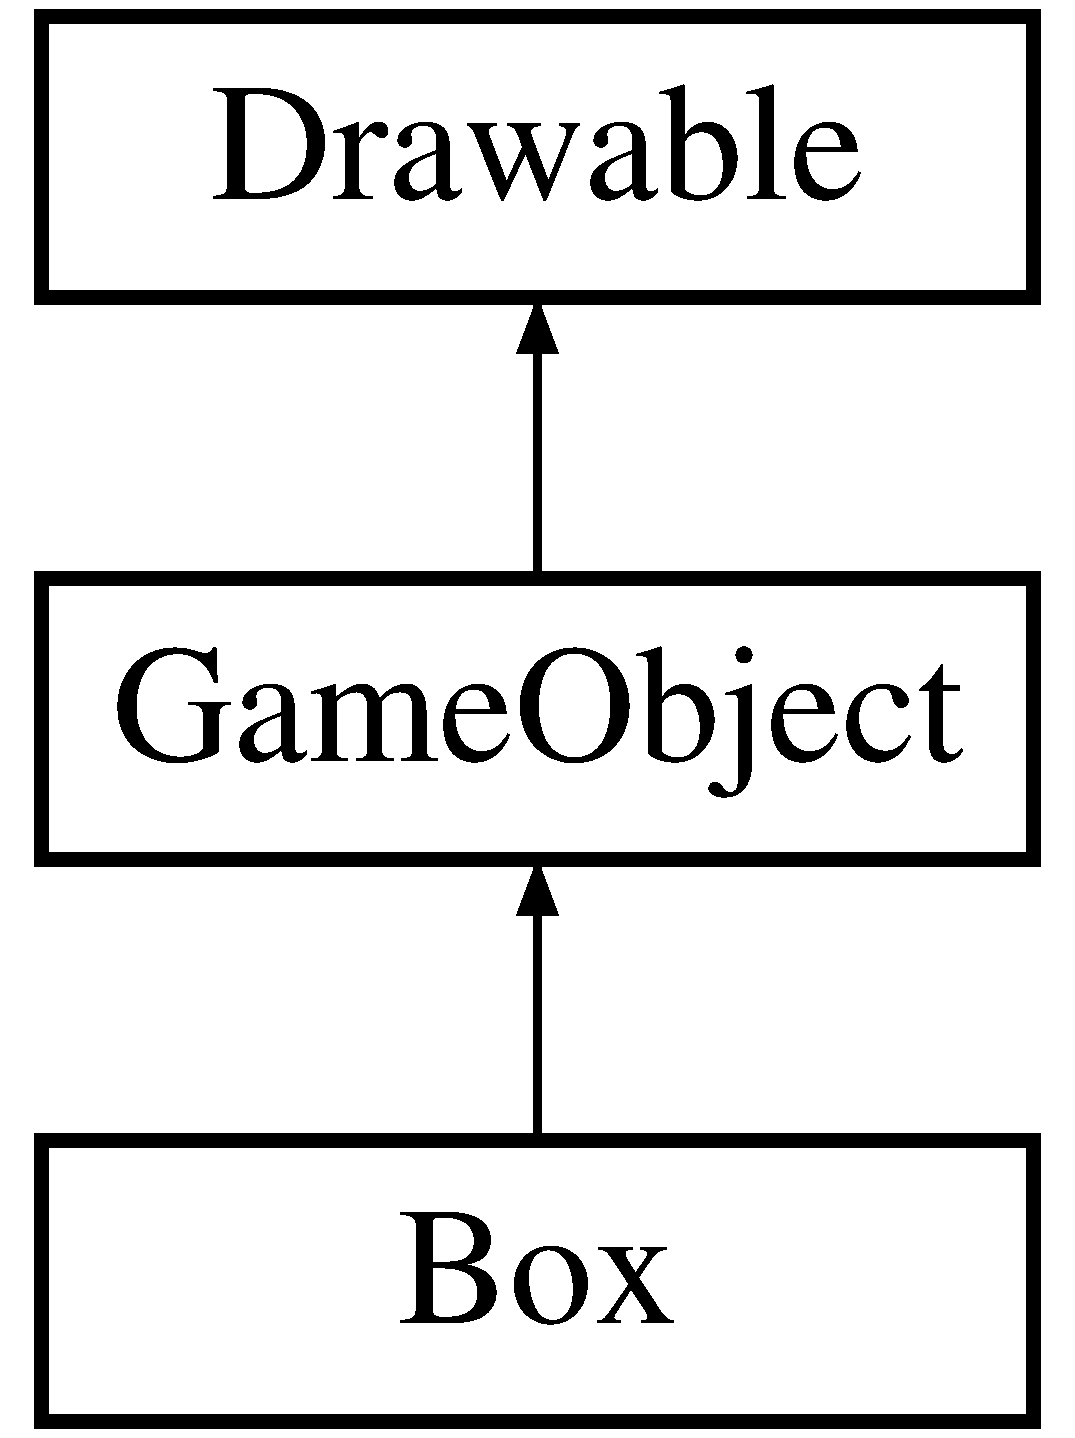
\includegraphics[height=3.000000cm]{class_box}
\end{center}
\end{figure}
\subsection*{Public Member Functions}
\begin{DoxyCompactItemize}
\item 
\hypertarget{class_box_aca78d7db44972bfa78d46b7bbc8796f6}{\hyperlink{class_box_aca78d7db44972bfa78d46b7bbc8796f6}{Box} ()}\label{class_box_aca78d7db44972bfa78d46b7bbc8796f6}

\begin{DoxyCompactList}\small\item\em Default constructor. \end{DoxyCompactList}\item 
\hyperlink{class_box_a11407004870f99a8b547e20d23bb5543}{Box} (const \hyperlink{class_vector2_d}{Vector2\+D}$<$ float $>$ \&k\+Pos, const \hyperlink{class_vector2_d}{Vector2\+D}$<$ float $>$ \&k\+Half)
\begin{DoxyCompactList}\small\item\em Constructor which takes position and half extents. \end{DoxyCompactList}\item 
\hypertarget{class_box_a84f26740f48268acf088360c0f288290}{virtual void \hyperlink{class_box_a84f26740f48268acf088360c0f288290}{transform} ()}\label{class_box_a84f26740f48268acf088360c0f288290}

\begin{DoxyCompactList}\small\item\em transforms the graphics shape \end{DoxyCompactList}\item 
virtual void \hyperlink{class_box_a170ec052134afb6dd70571b603d0e4a5}{draw} (sf\+::\+Render\+Target \&target, sf\+::\+Render\+States states) const 
\begin{DoxyCompactList}\small\item\em Draw the particle. \end{DoxyCompactList}\item 
void \hyperlink{class_box_ad83a96038d40168e90c3324e3b0125d3}{set\+Colour} (const sf\+::\+Color \&col)
\begin{DoxyCompactList}\small\item\em Sets the colour of the box. \end{DoxyCompactList}\end{DoxyCompactItemize}
\subsection*{Public Attributes}
\begin{DoxyCompactItemize}
\item 
\hypertarget{class_box_af7719c046c9377f48c020b5cbc763f85}{std\+::shared\+\_\+ptr$<$ \hyperlink{class_body2_d}{Body2\+D} $>$ \hyperlink{class_box_af7719c046c9377f48c020b5cbc763f85}{g\+\_\+p\+Body}}\label{class_box_af7719c046c9377f48c020b5cbc763f85}

\begin{DoxyCompactList}\small\item\em Pointer to physics body. \end{DoxyCompactList}\end{DoxyCompactItemize}
\subsection*{Additional Inherited Members}


\subsection{Detailed Description}
a non orientated physics body with a solid colour 

\subsection{Constructor \& Destructor Documentation}
\hypertarget{class_box_a11407004870f99a8b547e20d23bb5543}{\index{Box@{Box}!Box@{Box}}
\index{Box@{Box}!Box@{Box}}
\subsubsection[{Box}]{\setlength{\rightskip}{0pt plus 5cm}Box\+::\+Box (
\begin{DoxyParamCaption}
\item[{const {\bf Vector2\+D}$<$ float $>$ \&}]{k\+Pos, }
\item[{const {\bf Vector2\+D}$<$ float $>$ \&}]{k\+Half}
\end{DoxyParamCaption}
)}}\label{class_box_a11407004870f99a8b547e20d23bb5543}


Constructor which takes position and half extents. 


\begin{DoxyParams}{Parameters}
{\em k\+Pos} & Position \\
\hline
{\em k\+Half} & Half Extents \\
\hline
\end{DoxyParams}


\subsection{Member Function Documentation}
\hypertarget{class_box_a170ec052134afb6dd70571b603d0e4a5}{\index{Box@{Box}!draw@{draw}}
\index{draw@{draw}!Box@{Box}}
\subsubsection[{draw}]{\setlength{\rightskip}{0pt plus 5cm}void Box\+::draw (
\begin{DoxyParamCaption}
\item[{sf\+::\+Render\+Target \&}]{target, }
\item[{sf\+::\+Render\+States}]{states}
\end{DoxyParamCaption}
) const\hspace{0.3cm}{\ttfamily [virtual]}}}\label{class_box_a170ec052134afb6dd70571b603d0e4a5}


Draw the particle. 

$<$ Draw the particle \hypertarget{class_box_ad83a96038d40168e90c3324e3b0125d3}{\index{Box@{Box}!set\+Colour@{set\+Colour}}
\index{set\+Colour@{set\+Colour}!Box@{Box}}
\subsubsection[{set\+Colour}]{\setlength{\rightskip}{0pt plus 5cm}void Box\+::set\+Colour (
\begin{DoxyParamCaption}
\item[{const sf\+::\+Color \&}]{col}
\end{DoxyParamCaption}
)}}\label{class_box_ad83a96038d40168e90c3324e3b0125d3}


Sets the colour of the box. 


\begin{DoxyParams}{Parameters}
{\em col} & new colour \\
\hline
\end{DoxyParams}


The documentation for this class was generated from the following files\+:\begin{DoxyCompactItemize}
\item 
include/\hyperlink{_box_8h}{Box.\+h}\item 
src/\hyperlink{_box_8cpp}{Box.\+cpp}\end{DoxyCompactItemize}

\hypertarget{class_c_c}{\section{C\+C Class Reference}
\label{class_c_c}\index{C\+C@{C\+C}}
}


a circle shape which inherits from \hyperlink{class_physics_shape}{Physics\+Shape}  




{\ttfamily \#include $<$C\+C.\+h$>$}

Inheritance diagram for C\+C\+:\begin{figure}[H]
\begin{center}
\leavevmode
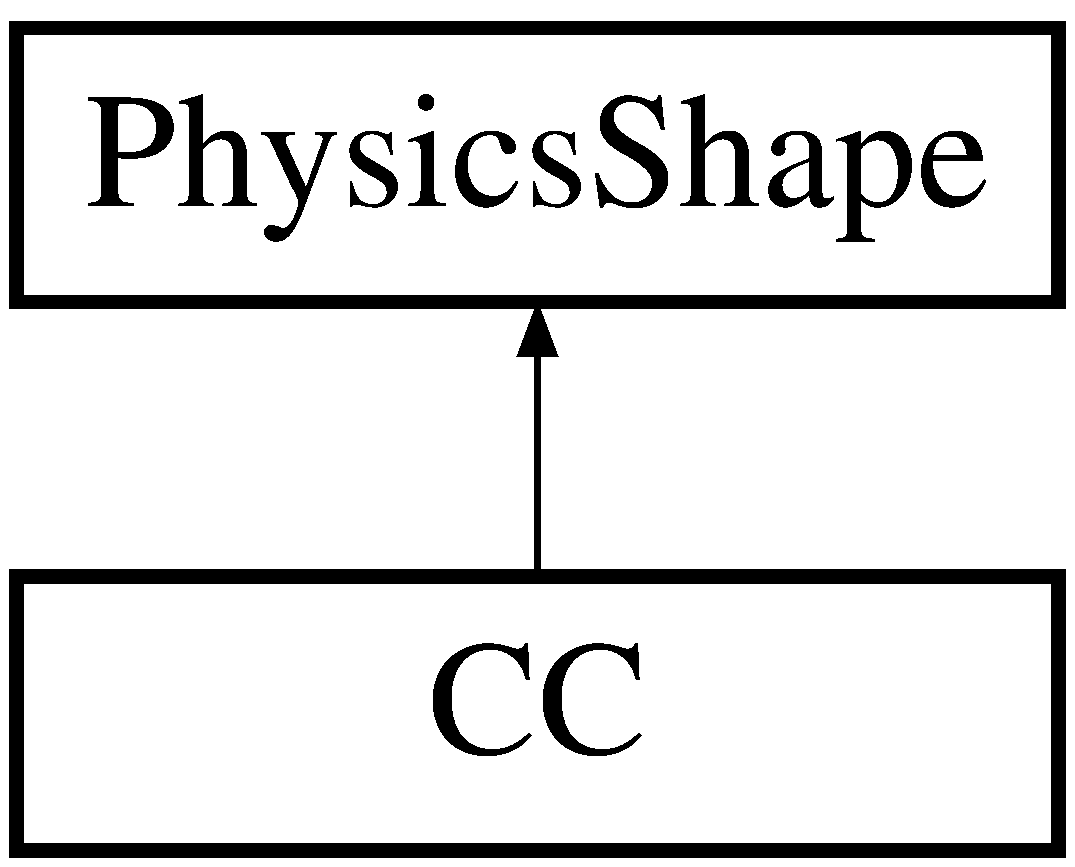
\includegraphics[height=2.000000cm]{class_c_c}
\end{center}
\end{figure}
\subsection*{Public Member Functions}
\begin{DoxyCompactItemize}
\item 
\hypertarget{class_c_c_a09cb54259760c46d58d5cb8719601af6}{\hyperlink{class_c_c_a09cb54259760c46d58d5cb8719601af6}{C\+C} ()}\label{class_c_c_a09cb54259760c46d58d5cb8719601af6}

\begin{DoxyCompactList}\small\item\em Default Constructor. \end{DoxyCompactList}\item 
\hyperlink{class_c_c_a4b3878b1ed23af886332d5d6d62d65c8}{C\+C} (const float kf\+Radius)
\begin{DoxyCompactList}\small\item\em Constructor which takes a radius value. \end{DoxyCompactList}\item 
void \hyperlink{class_c_c_a9b26f4420fa65278f93048ae62d4c154}{set\+Radius} (const float kf\+New\+Radius)
\begin{DoxyCompactList}\small\item\em Sets the radius of the circle. \end{DoxyCompactList}\item 
float \hyperlink{class_c_c_afe5cabbff942a13f20f5882258309fe3}{get\+Radius} () const 
\begin{DoxyCompactList}\small\item\em Returns the radius of the circle. \end{DoxyCompactList}\item 
virtual float \hyperlink{class_c_c_a26a40233a1bc78cd70bdcaff15ebc032}{compute\+Area} () const 
\begin{DoxyCompactList}\small\item\em Computes the area of the shape. \end{DoxyCompactList}\item 
\hypertarget{class_c_c_ac42c8589b3d366c4571c3898baa27b88}{virtual float \hyperlink{class_c_c_ac42c8589b3d366c4571c3898baa27b88}{compute\+Inertia} (const float kf\+Mass) const }\label{class_c_c_ac42c8589b3d366c4571c3898baa27b88}

\begin{DoxyCompactList}\small\item\em Virtual function to compute the area of the shape. \end{DoxyCompactList}\end{DoxyCompactItemize}
\subsection*{Protected Attributes}
\begin{DoxyCompactItemize}
\item 
float \hyperlink{class_c_c_af17ca41bf83fe08dd75a5957f7670787}{m\+\_\+f\+Radius}
\begin{DoxyCompactList}\small\item\em Computes the moment of inertia for the shape. \end{DoxyCompactList}\end{DoxyCompactItemize}


\subsection{Detailed Description}
a circle shape which inherits from \hyperlink{class_physics_shape}{Physics\+Shape} 

\subsection{Constructor \& Destructor Documentation}
\hypertarget{class_c_c_a4b3878b1ed23af886332d5d6d62d65c8}{\index{C\+C@{C\+C}!C\+C@{C\+C}}
\index{C\+C@{C\+C}!C\+C@{C\+C}}
\subsubsection[{C\+C}]{\setlength{\rightskip}{0pt plus 5cm}C\+C\+::\+C\+C (
\begin{DoxyParamCaption}
\item[{const float}]{kf\+Radius}
\end{DoxyParamCaption}
)}}\label{class_c_c_a4b3878b1ed23af886332d5d6d62d65c8}


Constructor which takes a radius value. 


\begin{DoxyParams}{Parameters}
{\em kf\+Radius} & Constructor which takes a radius value \\
\hline
\end{DoxyParams}


\subsection{Member Function Documentation}
\hypertarget{class_c_c_a26a40233a1bc78cd70bdcaff15ebc032}{\index{C\+C@{C\+C}!compute\+Area@{compute\+Area}}
\index{compute\+Area@{compute\+Area}!C\+C@{C\+C}}
\subsubsection[{compute\+Area}]{\setlength{\rightskip}{0pt plus 5cm}float C\+C\+::compute\+Area (
\begin{DoxyParamCaption}
{}
\end{DoxyParamCaption}
) const\hspace{0.3cm}{\ttfamily [virtual]}}}\label{class_c_c_a26a40233a1bc78cd70bdcaff15ebc032}


Computes the area of the shape. 

$<$ Computes the moment of inertia for the shape 

Reimplemented from \hyperlink{class_physics_shape_ae7bd37cc6d1c414e4d92649dba3cd791}{Physics\+Shape}.

\hypertarget{class_c_c_afe5cabbff942a13f20f5882258309fe3}{\index{C\+C@{C\+C}!get\+Radius@{get\+Radius}}
\index{get\+Radius@{get\+Radius}!C\+C@{C\+C}}
\subsubsection[{get\+Radius}]{\setlength{\rightskip}{0pt plus 5cm}float C\+C\+::get\+Radius (
\begin{DoxyParamCaption}
{}
\end{DoxyParamCaption}
) const}}\label{class_c_c_afe5cabbff942a13f20f5882258309fe3}


Returns the radius of the circle. 

$<$ Returns the radius of the circle \hypertarget{class_c_c_a9b26f4420fa65278f93048ae62d4c154}{\index{C\+C@{C\+C}!set\+Radius@{set\+Radius}}
\index{set\+Radius@{set\+Radius}!C\+C@{C\+C}}
\subsubsection[{set\+Radius}]{\setlength{\rightskip}{0pt plus 5cm}void C\+C\+::set\+Radius (
\begin{DoxyParamCaption}
\item[{const float}]{kf\+New\+Radius}
\end{DoxyParamCaption}
)}}\label{class_c_c_a9b26f4420fa65278f93048ae62d4c154}


Sets the radius of the circle. 


\begin{DoxyParams}{Parameters}
{\em kf\+New\+Radius} & Returns the radius of the circle \\
\hline
\end{DoxyParams}


\subsection{Member Data Documentation}
\hypertarget{class_c_c_af17ca41bf83fe08dd75a5957f7670787}{\index{C\+C@{C\+C}!m\+\_\+f\+Radius@{m\+\_\+f\+Radius}}
\index{m\+\_\+f\+Radius@{m\+\_\+f\+Radius}!C\+C@{C\+C}}
\subsubsection[{m\+\_\+f\+Radius}]{\setlength{\rightskip}{0pt plus 5cm}float C\+C\+::m\+\_\+f\+Radius\hspace{0.3cm}{\ttfamily [protected]}}}\label{class_c_c_af17ca41bf83fe08dd75a5957f7670787}


Computes the moment of inertia for the shape. 

Circle radius in meters 

The documentation for this class was generated from the following files\+:\begin{DoxyCompactItemize}
\item 
include/\hyperlink{_c_c_8h}{C\+C.\+h}\item 
src/\hyperlink{_c_c_8cpp}{C\+C.\+cpp}\end{DoxyCompactItemize}

\hypertarget{class_circular_bumper}{\section{Circular\+Bumper Class Reference}
\label{class_circular_bumper}\index{Circular\+Bumper@{Circular\+Bumper}}
}


a circular bumper which adds points to the score when hit  




{\ttfamily \#include $<$Circular\+Bumper.\+h$>$}

Inheritance diagram for Circular\+Bumper\+:\begin{figure}[H]
\begin{center}
\leavevmode
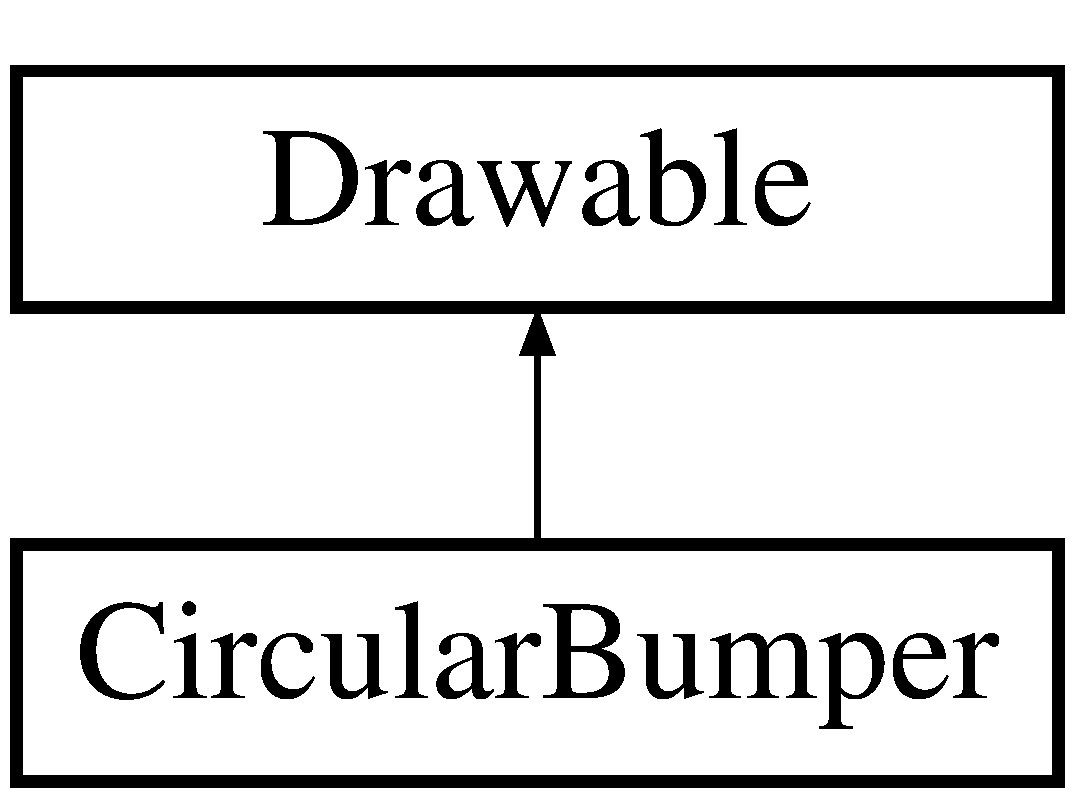
\includegraphics[height=2.000000cm]{class_circular_bumper}
\end{center}
\end{figure}
\subsection*{Public Member Functions}
\begin{DoxyCompactItemize}
\item 
\hypertarget{class_circular_bumper_a4b34986d6fa0dbaef189d87fac04ccfb}{\hyperlink{class_circular_bumper_a4b34986d6fa0dbaef189d87fac04ccfb}{Circular\+Bumper} ()}\label{class_circular_bumper_a4b34986d6fa0dbaef189d87fac04ccfb}

\begin{DoxyCompactList}\small\item\em Default constructor. \end{DoxyCompactList}\item 
\hyperlink{class_circular_bumper_af51b2361c3e0851abf547ccd305fded0}{Circular\+Bumper} (const \hyperlink{class_vector2_d}{Vector2\+D}$<$ float $>$ \&k\+Pos, const std\+::shared\+\_\+ptr$<$ \hyperlink{class_u_i_manager}{U\+I\+Manager} $>$ \&kp\+Point\+Counter, const unsigned int kui\+Pointvalue, const sf\+::\+Texture \&k\+Texture)
\begin{DoxyCompactList}\small\item\em Constructor which takes a position, a pointer to the points manager, a point value and a texture. \end{DoxyCompactList}\item 
virtual void \hyperlink{class_circular_bumper_a06077fa0e0bfdaa4b511cbd8f2a8c12d}{draw} (sf\+::\+Render\+Target \&target, sf\+::\+Render\+States states) const 
\begin{DoxyCompactList}\small\item\em Draw the bumper. \end{DoxyCompactList}\end{DoxyCompactItemize}
\subsection*{Public Attributes}
\begin{DoxyCompactItemize}
\item 
\hypertarget{class_circular_bumper_ade6659743e66c2e6db318753bef1e34a}{std\+::shared\+\_\+ptr$<$ \hyperlink{class_points_collider}{Points\+Collider} $>$ \hyperlink{class_circular_bumper_ade6659743e66c2e6db318753bef1e34a}{g\+\_\+p\+Body}}\label{class_circular_bumper_ade6659743e66c2e6db318753bef1e34a}

\begin{DoxyCompactList}\small\item\em Pointer to physics body. \end{DoxyCompactList}\end{DoxyCompactItemize}


\subsection{Detailed Description}
a circular bumper which adds points to the score when hit 

\subsection{Constructor \& Destructor Documentation}
\hypertarget{class_circular_bumper_af51b2361c3e0851abf547ccd305fded0}{\index{Circular\+Bumper@{Circular\+Bumper}!Circular\+Bumper@{Circular\+Bumper}}
\index{Circular\+Bumper@{Circular\+Bumper}!Circular\+Bumper@{Circular\+Bumper}}
\subsubsection[{Circular\+Bumper}]{\setlength{\rightskip}{0pt plus 5cm}Circular\+Bumper\+::\+Circular\+Bumper (
\begin{DoxyParamCaption}
\item[{const {\bf Vector2\+D}$<$ float $>$ \&}]{k\+Pos, }
\item[{const std\+::shared\+\_\+ptr$<$ {\bf U\+I\+Manager} $>$ \&}]{kp\+Point\+Counter, }
\item[{const unsigned int}]{kui\+Point\+Value, }
\item[{const sf\+::\+Texture \&}]{text}
\end{DoxyParamCaption}
)}}\label{class_circular_bumper_af51b2361c3e0851abf547ccd305fded0}


Constructor which takes a position, a pointer to the points manager, a point value and a texture. 


\begin{DoxyParams}{Parameters}
{\em k\+Pos} & Position value \\
\hline
{\em kp\+Point\+Counter} & Points manager \\
\hline
{\em kui\+Point\+Value} & Points value \\
\hline
{\em text} & Constructor which takes a position, a pointer to the points manager, a point value and a texture \\
\hline
\end{DoxyParams}


\subsection{Member Function Documentation}
\hypertarget{class_circular_bumper_a06077fa0e0bfdaa4b511cbd8f2a8c12d}{\index{Circular\+Bumper@{Circular\+Bumper}!draw@{draw}}
\index{draw@{draw}!Circular\+Bumper@{Circular\+Bumper}}
\subsubsection[{draw}]{\setlength{\rightskip}{0pt plus 5cm}void Circular\+Bumper\+::draw (
\begin{DoxyParamCaption}
\item[{sf\+::\+Render\+Target \&}]{target, }
\item[{sf\+::\+Render\+States}]{states}
\end{DoxyParamCaption}
) const\hspace{0.3cm}{\ttfamily [virtual]}}}\label{class_circular_bumper_a06077fa0e0bfdaa4b511cbd8f2a8c12d}


Draw the bumper. 

$<$ Draw the Bumper 

The documentation for this class was generated from the following files\+:\begin{DoxyCompactItemize}
\item 
include/\hyperlink{_circular_bumper_8h}{Circular\+Bumper.\+h}\item 
src/\hyperlink{_circular_bumper_8cpp}{Circular\+Bumper.\+cpp}\end{DoxyCompactItemize}

\hypertarget{struct_clamp_intersecting}{\section{Clamp\+Intersecting Struct Reference}
\label{struct_clamp_intersecting}\index{Clamp\+Intersecting@{Clamp\+Intersecting}}
}


contains clamp data  




{\ttfamily \#include $<$Collision2\+D.\+h$>$}

\subsection*{Public Attributes}
\begin{DoxyCompactItemize}
\item 
\hypertarget{struct_clamp_intersecting_a0ebcd8cbac2c6237228b0db439b514d4}{\hyperlink{class_vector2_d}{Vector2\+D}$<$ float $>$ \hyperlink{struct_clamp_intersecting_a0ebcd8cbac2c6237228b0db439b514d4}{clamp}}\label{struct_clamp_intersecting_a0ebcd8cbac2c6237228b0db439b514d4}

\begin{DoxyCompactList}\small\item\em Vector clamp value. \end{DoxyCompactList}\item 
\hypertarget{struct_clamp_intersecting_a7233e4f7677df0b463bb2b38d6cfeb64}{bool \hyperlink{struct_clamp_intersecting_a7233e4f7677df0b463bb2b38d6cfeb64}{b\+Intersecting}}\label{struct_clamp_intersecting_a7233e4f7677df0b463bb2b38d6cfeb64}

\begin{DoxyCompactList}\small\item\em True if the objects are intersecting. \end{DoxyCompactList}\end{DoxyCompactItemize}


\subsection{Detailed Description}
contains clamp data 

The documentation for this struct was generated from the following file\+:\begin{DoxyCompactItemize}
\item 
include/\hyperlink{_collision2_d_8h}{Collision2\+D.\+h}\end{DoxyCompactItemize}

\hypertarget{class_collision_manifold2_d}{\section{Collision\+Manifold2\+D Class Reference}
\label{class_collision_manifold2_d}\index{Collision\+Manifold2\+D@{Collision\+Manifold2\+D}}
}


Manifold generation for collisions, checks the collision and resolves it.  




{\ttfamily \#include $<$Collision2\+D.\+h$>$}

\subsection*{Public Member Functions}
\begin{DoxyCompactItemize}
\item 
\hyperlink{class_collision_manifold2_d_af6120e277cf4d8d5b6cc2a67e621c45d}{Collision\+Manifold2\+D} (const std\+::shared\+\_\+ptr$<$ \hyperlink{class_body2_d}{Body2\+D} $>$ \&kp\+Body1, const std\+::shared\+\_\+ptr$<$ \hyperlink{class_body2_d}{Body2\+D} $>$ \&kp\+Body2)
\item 
\hyperlink{struct_clamp_intersecting}{Clamp\+Intersecting} \hyperlink{class_collision_manifold2_d_a0f1383fe1b5c73b8d638b2baaf08219f}{Clamp} (const \hyperlink{class_vector2_d}{Vector2\+D}$<$ float $>$ \&k\+Dist, const \hyperlink{class_vector2_d}{Vector2\+D}$<$ float $>$ \&k\+Half\+Extents) const 
\begin{DoxyCompactList}\small\item\em Constructor which takes two body pointers. \end{DoxyCompactList}\item 
const \hyperlink{class_vector2_d}{Vector2\+D}$<$ float $>$ \hyperlink{class_collision_manifold2_d_a417217e2fcbb175cbb18577760466ea8}{distance} () const 
\begin{DoxyCompactList}\small\item\em Distance between the bodies. \end{DoxyCompactList}\item 
\hypertarget{class_collision_manifold2_d_a2cc491b84be92c80fb1ab17eb4140c7e}{bool \hyperlink{class_collision_manifold2_d_a2cc491b84be92c80fb1ab17eb4140c7e}{check\+Collision} ()}\label{class_collision_manifold2_d_a2cc491b84be92c80fb1ab17eb4140c7e}

\begin{DoxyCompactList}\small\item\em Check if the objects are colliding. \end{DoxyCompactList}\item 
\hypertarget{class_collision_manifold2_d_a0037327cbc9544ba24a6aafb5dec5855}{bool \hyperlink{class_collision_manifold2_d_a0037327cbc9544ba24a6aafb5dec5855}{A\+A\+B\+Bvs\+A\+A\+B\+B} ()}\label{class_collision_manifold2_d_a0037327cbc9544ba24a6aafb5dec5855}

\begin{DoxyCompactList}\small\item\em Check collision between two A\+A\+B\+Bs. \end{DoxyCompactList}\item 
\hypertarget{class_collision_manifold2_d_a3f9c9ef16199d2ed12ff50bd7b5cccac}{bool \hyperlink{class_collision_manifold2_d_a3f9c9ef16199d2ed12ff50bd7b5cccac}{Circle\+Vs\+Circle} ()}\label{class_collision_manifold2_d_a3f9c9ef16199d2ed12ff50bd7b5cccac}

\begin{DoxyCompactList}\small\item\em Check collision between two Circles. \end{DoxyCompactList}\item 
\hypertarget{class_collision_manifold2_d_a48419f339540ce108582ed1ba28021a7}{bool \hyperlink{class_collision_manifold2_d_a48419f339540ce108582ed1ba28021a7}{A\+A\+B\+B\+Vs\+Circle} ()}\label{class_collision_manifold2_d_a48419f339540ce108582ed1ba28021a7}

\begin{DoxyCompactList}\small\item\em Check collision between an \hyperlink{class_a_a_b_b}{A\+A\+B\+B} and circle. \end{DoxyCompactList}\item 
\hypertarget{class_collision_manifold2_d_aac3dc83ebb8919c2ea37902dff315c93}{bool \hyperlink{class_collision_manifold2_d_aac3dc83ebb8919c2ea37902dff315c93}{O\+B\+B\+Vs\+Circle} ()}\label{class_collision_manifold2_d_aac3dc83ebb8919c2ea37902dff315c93}

\begin{DoxyCompactList}\small\item\em Check collision between an \hyperlink{class_o_b_b}{O\+B\+B} and circle. \end{DoxyCompactList}\item 
\hypertarget{class_collision_manifold2_d_ad6392d7e37396c279ec3f3bd926d1c1a}{void \hyperlink{class_collision_manifold2_d_ad6392d7e37396c279ec3f3bd926d1c1a}{resolve\+Rotational\+Collision} ()}\label{class_collision_manifold2_d_ad6392d7e37396c279ec3f3bd926d1c1a}

\begin{DoxyCompactList}\small\item\em Resolve a collision. \end{DoxyCompactList}\item 
\hypertarget{class_collision_manifold2_d_a427412801fdb0747a9f56923a87642f2}{void \hyperlink{class_collision_manifold2_d_a427412801fdb0747a9f56923a87642f2}{Positional\+Correction} ()}\label{class_collision_manifold2_d_a427412801fdb0747a9f56923a87642f2}

\begin{DoxyCompactList}\small\item\em Apply position correction. \end{DoxyCompactList}\end{DoxyCompactItemize}
\subsection*{Public Attributes}
\begin{DoxyCompactItemize}
\item 
\hypertarget{class_collision_manifold2_d_a3cb8f07a11c1510e90ecfd7057bac132}{std\+::shared\+\_\+ptr$<$ \hyperlink{class_body2_d}{Body2\+D} $>$ \hyperlink{class_collision_manifold2_d_a3cb8f07a11c1510e90ecfd7057bac132}{g\+\_\+p\+Body\+A}}\label{class_collision_manifold2_d_a3cb8f07a11c1510e90ecfd7057bac132}

\begin{DoxyCompactList}\small\item\em First body in the manifold. \end{DoxyCompactList}\item 
\hypertarget{class_collision_manifold2_d_a984686fec2c7460f9479c12987392ada}{std\+::shared\+\_\+ptr$<$ \hyperlink{class_body2_d}{Body2\+D} $>$ \hyperlink{class_collision_manifold2_d_a984686fec2c7460f9479c12987392ada}{g\+\_\+p\+Body\+B}}\label{class_collision_manifold2_d_a984686fec2c7460f9479c12987392ada}

\begin{DoxyCompactList}\small\item\em Second body in the manifold. \end{DoxyCompactList}\item 
\hypertarget{class_collision_manifold2_d_a6c9c40573b42b63f54a44eed63f279b0}{\hyperlink{class_vector2_d}{Vector2\+D}$<$ float $>$ \hyperlink{class_collision_manifold2_d_a6c9c40573b42b63f54a44eed63f279b0}{g\+\_\+\+Point\+Of\+Contact}}\label{class_collision_manifold2_d_a6c9c40573b42b63f54a44eed63f279b0}

\begin{DoxyCompactList}\small\item\em Collision contact point. \end{DoxyCompactList}\item 
\hypertarget{class_collision_manifold2_d_af11f8fdabd6c64cd5637cfbb6de4777d}{float \hyperlink{class_collision_manifold2_d_af11f8fdabd6c64cd5637cfbb6de4777d}{g\+\_\+f\+Radius}}\label{class_collision_manifold2_d_af11f8fdabd6c64cd5637cfbb6de4777d}

\begin{DoxyCompactList}\small\item\em Radius sum set when an object isn't colliding with a body with an attractive value. \end{DoxyCompactList}\item 
\hypertarget{class_collision_manifold2_d_a7723c5a4ef26168b35d68c2d437c7dde}{float \hyperlink{class_collision_manifold2_d_a7723c5a4ef26168b35d68c2d437c7dde}{g\+\_\+f\+Penetration}}\label{class_collision_manifold2_d_a7723c5a4ef26168b35d68c2d437c7dde}

\begin{DoxyCompactList}\small\item\em Penetration of the collision. \end{DoxyCompactList}\item 
\hypertarget{class_collision_manifold2_d_a546b4ca4cca3062814ad99695dc38c26}{\hyperlink{class_vector2_d}{Vector2\+D}$<$ float $>$ \hyperlink{class_collision_manifold2_d_a546b4ca4cca3062814ad99695dc38c26}{g\+\_\+\+Normal}}\label{class_collision_manifold2_d_a546b4ca4cca3062814ad99695dc38c26}

\begin{DoxyCompactList}\small\item\em Collision normal. \end{DoxyCompactList}\end{DoxyCompactItemize}


\subsection{Detailed Description}
Manifold generation for collisions, checks the collision and resolves it. 

\subsection{Constructor \& Destructor Documentation}
\hypertarget{class_collision_manifold2_d_af6120e277cf4d8d5b6cc2a67e621c45d}{\index{Collision\+Manifold2\+D@{Collision\+Manifold2\+D}!Collision\+Manifold2\+D@{Collision\+Manifold2\+D}}
\index{Collision\+Manifold2\+D@{Collision\+Manifold2\+D}!Collision\+Manifold2\+D@{Collision\+Manifold2\+D}}
\subsubsection[{Collision\+Manifold2\+D}]{\setlength{\rightskip}{0pt plus 5cm}Collision\+Manifold2\+D\+::\+Collision\+Manifold2\+D (
\begin{DoxyParamCaption}
\item[{const std\+::shared\+\_\+ptr$<$ {\bf Body2\+D} $>$ \&}]{kp\+Body1, }
\item[{const std\+::shared\+\_\+ptr$<$ {\bf Body2\+D} $>$ \&}]{kp\+Body2}
\end{DoxyParamCaption}
)\hspace{0.3cm}{\ttfamily [inline]}}}\label{class_collision_manifold2_d_af6120e277cf4d8d5b6cc2a67e621c45d}

\begin{DoxyParams}{Parameters}
{\em kp\+Body2} & Second body \\
\hline
\end{DoxyParams}


\subsection{Member Function Documentation}
\hypertarget{class_collision_manifold2_d_a0f1383fe1b5c73b8d638b2baaf08219f}{\index{Collision\+Manifold2\+D@{Collision\+Manifold2\+D}!Clamp@{Clamp}}
\index{Clamp@{Clamp}!Collision\+Manifold2\+D@{Collision\+Manifold2\+D}}
\subsubsection[{Clamp}]{\setlength{\rightskip}{0pt plus 5cm}{\bf Clamp\+Intersecting} Collision\+Manifold2\+D\+::\+Clamp (
\begin{DoxyParamCaption}
\item[{const {\bf Vector2\+D}$<$ float $>$ \&}]{k\+Dist, }
\item[{const {\bf Vector2\+D}$<$ float $>$ \&}]{k\+Half\+Extents}
\end{DoxyParamCaption}
) const}}\label{class_collision_manifold2_d_a0f1383fe1b5c73b8d638b2baaf08219f}


Constructor which takes two body pointers. 

$<$ Clamp a circle to the half extents of a box

Clamp a circle to the half extents of a box 
\begin{DoxyParams}{Parameters}
{\em k\+Dist} & Distance \\
\hline
{\em k\+Half\+Extents} & Halfextents \\
\hline
\end{DoxyParams}
\hypertarget{class_collision_manifold2_d_a417217e2fcbb175cbb18577760466ea8}{\index{Collision\+Manifold2\+D@{Collision\+Manifold2\+D}!distance@{distance}}
\index{distance@{distance}!Collision\+Manifold2\+D@{Collision\+Manifold2\+D}}
\subsubsection[{distance}]{\setlength{\rightskip}{0pt plus 5cm}const {\bf Vector2\+D}$<$ float $>$ Collision\+Manifold2\+D\+::distance (
\begin{DoxyParamCaption}
{}
\end{DoxyParamCaption}
) const}}\label{class_collision_manifold2_d_a417217e2fcbb175cbb18577760466ea8}


Distance between the bodies. 

$<$ Distance between the bodies 

The documentation for this class was generated from the following files\+:\begin{DoxyCompactItemize}
\item 
include/\hyperlink{_collision2_d_8h}{Collision2\+D.\+h}\item 
src/\hyperlink{collision2_d_8cpp}{collision2\+D.\+cpp}\end{DoxyCompactItemize}

\hypertarget{class_game_object}{\section{Game\+Object Class Reference}
\label{class_game_object}\index{Game\+Object@{Game\+Object}}
}


a game drawable object with a game object type  




{\ttfamily \#include $<$Game\+Object.\+h$>$}

Inheritance diagram for Game\+Object\+:\begin{figure}[H]
\begin{center}
\leavevmode
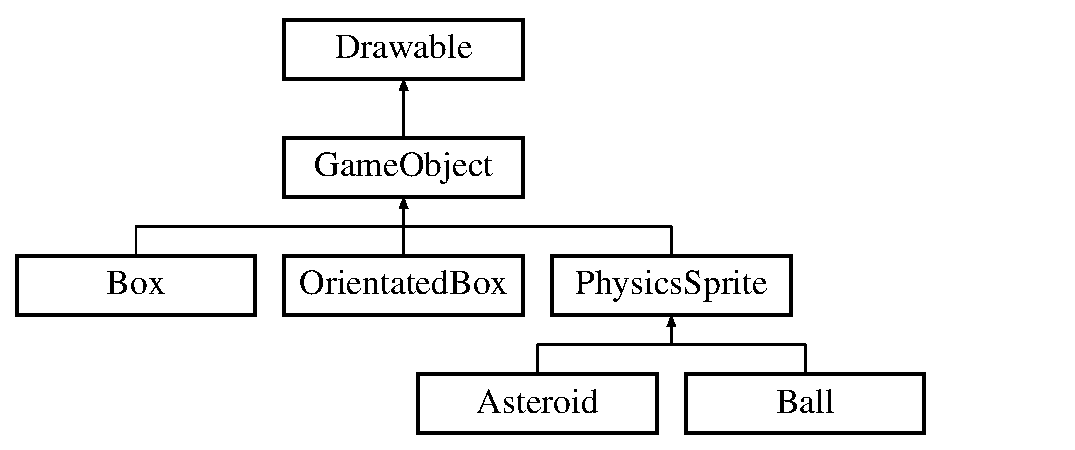
\includegraphics[height=4.000000cm]{class_game_object}
\end{center}
\end{figure}
\subsection*{Public Member Functions}
\begin{DoxyCompactItemize}
\item 
\hypertarget{class_game_object_a93dd079d4f47880491665b4a83eb687d}{virtual void \hyperlink{class_game_object_a93dd079d4f47880491665b4a83eb687d}{transform} ()}\label{class_game_object_a93dd079d4f47880491665b4a83eb687d}

\begin{DoxyCompactList}\small\item\em Default Constructor. \end{DoxyCompactList}\item 
\hypertarget{class_game_object_af7a8fd8ce2f6955b378e2292f2475e4d}{\hyperlink{_game_config_8h_a57678b60d65afb213d04a6b090c64a08}{Game\+Object\+Type} \hyperlink{class_game_object_af7a8fd8ce2f6955b378e2292f2475e4d}{get\+Object\+Type} () const }\label{class_game_object_af7a8fd8ce2f6955b378e2292f2475e4d}

\begin{DoxyCompactList}\small\item\em Transform the graphics. \end{DoxyCompactList}\end{DoxyCompactItemize}
\subsection*{Protected Attributes}
\begin{DoxyCompactItemize}
\item 
\hypertarget{class_game_object_a31b42727d57825d194e345cc30157401}{\hyperlink{_game_config_8h_a57678b60d65afb213d04a6b090c64a08}{Game\+Object\+Type} \hyperlink{class_game_object_a31b42727d57825d194e345cc30157401}{m\+\_\+\+Object\+Type}}\label{class_game_object_a31b42727d57825d194e345cc30157401}

\begin{DoxyCompactList}\small\item\em Game object type, set by children. \end{DoxyCompactList}\end{DoxyCompactItemize}


\subsection{Detailed Description}
a game drawable object with a game object type 

The documentation for this class was generated from the following file\+:\begin{DoxyCompactItemize}
\item 
include/\hyperlink{_game_object_8h}{Game\+Object.\+h}\end{DoxyCompactItemize}

\hypertarget{class_game_scene}{\section{Game\+Scene Class Reference}
\label{class_game_scene}\index{Game\+Scene@{Game\+Scene}}
}


a game scene with a physics world  




{\ttfamily \#include $<$Game\+Scene.\+h$>$}

Inheritance diagram for Game\+Scene\+:\begin{figure}[H]
\begin{center}
\leavevmode
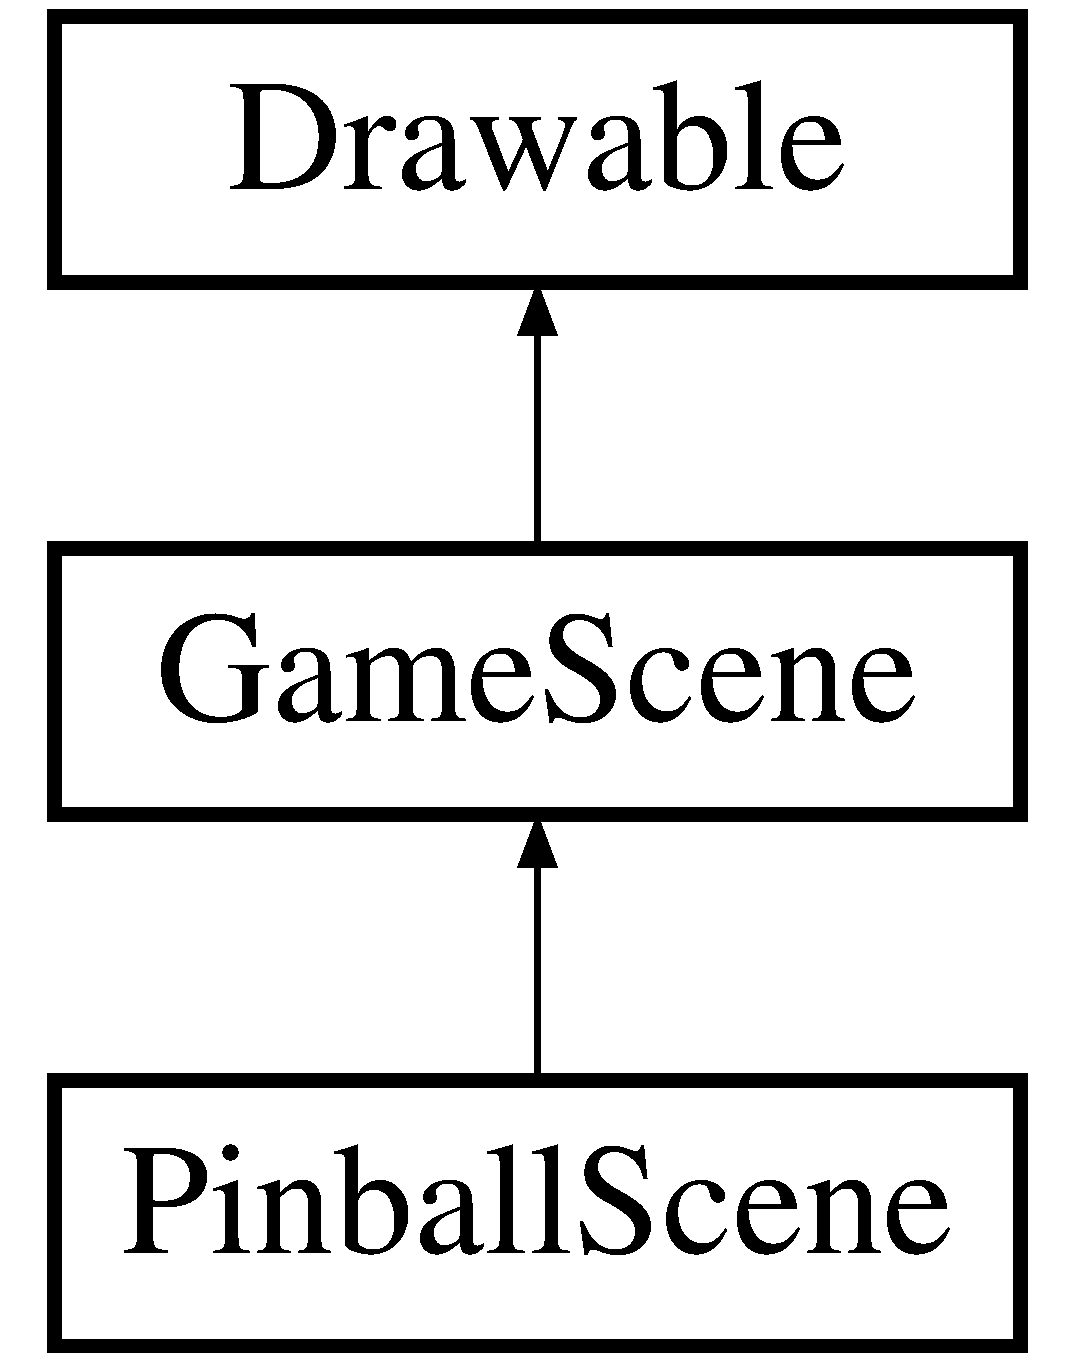
\includegraphics[height=3.000000cm]{class_game_scene}
\end{center}
\end{figure}
\subsection*{Public Member Functions}
\begin{DoxyCompactItemize}
\item 
\hypertarget{class_game_scene_ad0aa729b9dba3a8e09b2a8a61fcb3dce}{virtual void {\bfseries update} ()}\label{class_game_scene_ad0aa729b9dba3a8e09b2a8a61fcb3dce}

\item 
virtual void \hyperlink{class_game_scene_a9cf68fbf8e0805cbb1618a71e04d7fa4}{event} (sf\+::\+Event event)
\begin{DoxyCompactList}\small\item\em Update the game logic. \end{DoxyCompactList}\item 
\hypertarget{class_game_scene_a9b7472887a15c9c93f020d56872f8968}{virtual void {\bfseries draw} (sf\+::\+Render\+Target \&target, sf\+::\+Render\+States states) const }\label{class_game_scene_a9b7472887a15c9c93f020d56872f8968}

\end{DoxyCompactItemize}
\subsection*{Protected Attributes}
\begin{DoxyCompactItemize}
\item 
\hypertarget{class_game_scene_a887137cff9aa0c98abf922bffdc244dc}{sf\+::\+Clock \hyperlink{class_game_scene_a887137cff9aa0c98abf922bffdc244dc}{m\+\_\+timer}}\label{class_game_scene_a887137cff9aa0c98abf922bffdc244dc}

\begin{DoxyCompactList}\small\item\em Gameloop timer. \end{DoxyCompactList}\item 
\hypertarget{class_game_scene_ac1e2df8edcb25aaeddc2b1805e5c48d1}{float \hyperlink{class_game_scene_ac1e2df8edcb25aaeddc2b1805e5c48d1}{m\+\_\+f\+Accumulator}}\label{class_game_scene_ac1e2df8edcb25aaeddc2b1805e5c48d1}

\begin{DoxyCompactList}\small\item\em Time accumulator. \end{DoxyCompactList}\item 
\hypertarget{class_game_scene_a90073e2f9e2e404c04ccfa36039acade}{float \hyperlink{class_game_scene_a90073e2f9e2e404c04ccfa36039acade}{m\+\_\+f\+Previous\+Frame}}\label{class_game_scene_a90073e2f9e2e404c04ccfa36039acade}

\begin{DoxyCompactList}\small\item\em Previous frame time. \end{DoxyCompactList}\item 
\hypertarget{class_game_scene_acf69304d0b55c0190a70d349aba63840}{\hyperlink{class_world2_d}{World2\+D} \hyperlink{class_game_scene_acf69304d0b55c0190a70d349aba63840}{m\+\_\+\+World}}\label{class_game_scene_acf69304d0b55c0190a70d349aba63840}

\begin{DoxyCompactList}\small\item\em Physics world. \end{DoxyCompactList}\end{DoxyCompactItemize}


\subsection{Detailed Description}
a game scene with a physics world 

\subsection{Member Function Documentation}
\hypertarget{class_game_scene_a9cf68fbf8e0805cbb1618a71e04d7fa4}{\index{Game\+Scene@{Game\+Scene}!event@{event}}
\index{event@{event}!Game\+Scene@{Game\+Scene}}
\subsubsection[{event}]{\setlength{\rightskip}{0pt plus 5cm}virtual void Game\+Scene\+::event (
\begin{DoxyParamCaption}
\item[{sf\+::\+Event}]{event}
\end{DoxyParamCaption}
)\hspace{0.3cm}{\ttfamily [inline]}, {\ttfamily [virtual]}}}\label{class_game_scene_a9cf68fbf8e0805cbb1618a71e04d7fa4}


Update the game logic. 


\begin{DoxyParams}{Parameters}
{\em event} & Handles S\+F\+M\+L events \\
\hline
\end{DoxyParams}


Reimplemented in \hyperlink{class_pinball_scene_a57947a5d74f53f73a40df59de2c72078}{Pinball\+Scene}.



The documentation for this class was generated from the following file\+:\begin{DoxyCompactItemize}
\item 
include/\hyperlink{_game_scene_8h}{Game\+Scene.\+h}\end{DoxyCompactItemize}

\hypertarget{struct_image_with_name}{\section{Image\+With\+Name Struct Reference}
\label{struct_image_with_name}\index{Image\+With\+Name@{Image\+With\+Name}}
}


structure which contains textures and their associated file name  




{\ttfamily \#include $<$Sprite\+Manager.\+h$>$}

\subsection*{Public Attributes}
\begin{DoxyCompactItemize}
\item 
\hypertarget{struct_image_with_name_a31c52b6a208c5dc8440031c4f76afa63}{sf\+::\+Texture \hyperlink{struct_image_with_name_a31c52b6a208c5dc8440031c4f76afa63}{m\+\_\+texture}}\label{struct_image_with_name_a31c52b6a208c5dc8440031c4f76afa63}

\begin{DoxyCompactList}\small\item\em Texture. \end{DoxyCompactList}\item 
\hypertarget{struct_image_with_name_ae911332d5a2772f20e49f3d5d670b966}{std\+::string \hyperlink{struct_image_with_name_ae911332d5a2772f20e49f3d5d670b966}{m\+\_\+name}}\label{struct_image_with_name_ae911332d5a2772f20e49f3d5d670b966}

\begin{DoxyCompactList}\small\item\em Texture file name. \end{DoxyCompactList}\end{DoxyCompactItemize}


\subsection{Detailed Description}
structure which contains textures and their associated file name 

\hyperlink{struct_image_with_name}{Image\+With\+Name} 

The documentation for this struct was generated from the following file\+:\begin{DoxyCompactItemize}
\item 
include/\hyperlink{_sprite_manager_8h}{Sprite\+Manager.\+h}\end{DoxyCompactItemize}

\hypertarget{struct_mass_data}{\section{Mass\+Data Struct Reference}
\label{struct_mass_data}\index{Mass\+Data@{Mass\+Data}}
}


{\ttfamily \#include $<$Body2\+D.\+h$>$}

\subsection*{Public Attributes}
\begin{DoxyCompactItemize}
\item 
\hypertarget{struct_mass_data_a7c28659bb358f0a22fb909dc394e51af}{float \hyperlink{struct_mass_data_a7c28659bb358f0a22fb909dc394e51af}{f\+Mass}}\label{struct_mass_data_a7c28659bb358f0a22fb909dc394e51af}

\begin{DoxyCompactList}\small\item\em Float Mass. \end{DoxyCompactList}\item 
\hypertarget{struct_mass_data_a927ec9b0975da4fe138f3dcae2ee9c41}{float \hyperlink{struct_mass_data_a927ec9b0975da4fe138f3dcae2ee9c41}{f\+Inv\+Mass}}\label{struct_mass_data_a927ec9b0975da4fe138f3dcae2ee9c41}

\begin{DoxyCompactList}\small\item\em Float Inverse Mass. \end{DoxyCompactList}\item 
\hypertarget{struct_mass_data_acb9e284ee199bb53de8bd24db5716959}{float \hyperlink{struct_mass_data_acb9e284ee199bb53de8bd24db5716959}{f\+Attractive\+Value}}\label{struct_mass_data_acb9e284ee199bb53de8bd24db5716959}

\begin{DoxyCompactList}\small\item\em Float scalar of how much other objects are attracted to the body. \end{DoxyCompactList}\end{DoxyCompactItemize}


\subsection{Detailed Description}
structure which stores information on mass 

The documentation for this struct was generated from the following file\+:\begin{DoxyCompactItemize}
\item 
include/\hyperlink{_body2_d_8h}{Body2\+D.\+h}\end{DoxyCompactItemize}

\hypertarget{struct_material}{\section{Material Struct Reference}
\label{struct_material}\index{Material@{Material}}
}


{\ttfamily \#include $<$Body2\+D.\+h$>$}

\subsection*{Public Attributes}
\begin{DoxyCompactItemize}
\item 
\hypertarget{struct_material_ab3ed6198749e068421eb6ca9142bf66d}{float \hyperlink{struct_material_ab3ed6198749e068421eb6ca9142bf66d}{f\+Density}}\label{struct_material_ab3ed6198749e068421eb6ca9142bf66d}

\begin{DoxyCompactList}\small\item\em Float Density. \end{DoxyCompactList}\item 
\hypertarget{struct_material_a1a2b4a0a84de4e6e9bc8f52847453e5c}{float \hyperlink{struct_material_a1a2b4a0a84de4e6e9bc8f52847453e5c}{f\+Restitution}}\label{struct_material_a1a2b4a0a84de4e6e9bc8f52847453e5c}

\begin{DoxyCompactList}\small\item\em Float Restitution. \end{DoxyCompactList}\item 
\hypertarget{struct_material_a48fcaa790747f9402d48017cae285a98}{float \hyperlink{struct_material_a48fcaa790747f9402d48017cae285a98}{f\+Friction}}\label{struct_material_a48fcaa790747f9402d48017cae285a98}

\begin{DoxyCompactList}\small\item\em Float friction. \end{DoxyCompactList}\end{DoxyCompactItemize}


\subsection{Detailed Description}
structure which stores information on the material 

The documentation for this struct was generated from the following file\+:\begin{DoxyCompactItemize}
\item 
include/\hyperlink{_body2_d_8h}{Body2\+D.\+h}\end{DoxyCompactItemize}

\hypertarget{class_matrix}{\section{Matrix$<$ N $>$ Class Template Reference}
\label{class_matrix}\index{Matrix$<$ N $>$@{Matrix$<$ N $>$}}
}


A 2\+D matrix template.  




{\ttfamily \#include $<$Matrix.\+h$>$}

\subsection*{Public Member Functions}
\begin{DoxyCompactItemize}
\item 
\hyperlink{class_matrix_aad1599c87ef31d073c2bb38d9ef955b6}{Matrix} (const unsigned int kui\+Size)
\begin{DoxyCompactList}\small\item\em Default constructor. \end{DoxyCompactList}\item 
\hyperlink{class_matrix_aac2bcab1b31e9521c361c56aa4ae00f6}{Matrix} (const unsigned int kui\+Row\+Size, const unsigned int kui\+Column\+Size)
\begin{DoxyCompactList}\small\item\em Constructor which takes an unsigned integer which sets the size of the N and M axies. \end{DoxyCompactList}\item 
N \hyperlink{class_matrix_ac91fbcc1cace5ea4c67252e798a942ba}{get\+Num} (const unsigned int kui\+Row, const unsigned int kui\+Column) const 
\begin{DoxyCompactList}\small\item\em Constructor which takes two unsigned integers which sets the size of the N and M axies. \end{DoxyCompactList}\item 
void \hyperlink{class_matrix_a841bb352aabe6b8d5492324eaa6b63c6}{set\+Num} (N number, const unsigned int kui\+Row, const unsigned int kui\+Column)
\begin{DoxyCompactList}\small\item\em Returns the value at a position. \end{DoxyCompactList}\item 
\hypertarget{class_matrix_aa7f14b67329eb92cac86797dc6a2be2c}{unsigned long \hyperlink{class_matrix_aa7f14b67329eb92cac86797dc6a2be2c}{get\+Row\+Size} () const }\label{class_matrix_aa7f14b67329eb92cac86797dc6a2be2c}

\begin{DoxyCompactList}\small\item\em Sets the value at a position. \end{DoxyCompactList}\item 
\hypertarget{class_matrix_a34f1b73377895cf211fd28e8103e9e19}{unsigned long \hyperlink{class_matrix_a34f1b73377895cf211fd28e8103e9e19}{get\+Column\+Size} () const }\label{class_matrix_a34f1b73377895cf211fd28e8103e9e19}

\begin{DoxyCompactList}\small\item\em Returns the size of the rows. \end{DoxyCompactList}\item 
void \hyperlink{class_matrix_a08e8d5924967ddaa167d0f7900d91236}{set\+Size} (const unsigned int kui\+Row\+Size, const unsigned int kui\+Column\+Size)
\begin{DoxyCompactList}\small\item\em Returns the size of the columns. \end{DoxyCompactList}\item 
\hypertarget{class_matrix_a838aaaeed045076e77234cf91d76cf5e}{\hyperlink{class_matrix}{Matrix}$<$ N $>$ \& \hyperlink{class_matrix_a838aaaeed045076e77234cf91d76cf5e}{identity\+Matrix} ()}\label{class_matrix_a838aaaeed045076e77234cf91d76cf5e}

\begin{DoxyCompactList}\small\item\em Sets the size of the matrix. \end{DoxyCompactList}\item 
\hyperlink{class_matrix}{Matrix}$<$ N $>$ \hyperlink{class_matrix_a2136b90f9ac8b15c3d01873c7505a5ca}{operator+} (const \hyperlink{class_matrix}{Matrix}$<$ N $>$ $\ast$kp\+Other) const 
\begin{DoxyCompactList}\small\item\em Sets the matrix to the identity matrix. \end{DoxyCompactList}\item 
\hyperlink{class_matrix}{Matrix}$<$ N $>$ \hyperlink{class_matrix_ab43f0fe9ef6d2fb13e4b320faa9309ad}{operator-\/} (const \hyperlink{class_matrix}{Matrix}$<$ N $>$ $\ast$kp\+Other) const 
\begin{DoxyCompactList}\small\item\em Returns the current matrix minus another matrix. \end{DoxyCompactList}\item 
\hyperlink{class_matrix}{Matrix}$<$ N $>$ \hyperlink{class_matrix_a2f45d0a6c687b34e8392b1683b497f2b}{operator$\ast$} (const \hyperlink{class_matrix}{Matrix}$<$ N $>$ $\ast$kp\+Other) const 
\begin{DoxyCompactList}\small\item\em Returns the current matrix multiplied by another matrix. \end{DoxyCompactList}\item 
\hyperlink{class_matrix}{Matrix}$<$ N $>$ \hyperlink{class_matrix_a78d0b17326e06680d3235f56cbb07eeb}{operator$\ast$} (const float kf\+Scalar) const 
\begin{DoxyCompactList}\small\item\em Returns the current matrix multiplied by a scalar. \end{DoxyCompactList}\item 
\hyperlink{class_matrix}{Matrix}$<$ N $>$ \& \hyperlink{class_matrix_aa0b29bc78592dba6988b7671c834645b}{operator=} (const \hyperlink{class_matrix}{Matrix} $\ast$kp\+Other)
\begin{DoxyCompactList}\small\item\em Assignment operator. \end{DoxyCompactList}\end{DoxyCompactItemize}


\subsection{Detailed Description}
\subsubsection*{template$<$class N$>$class Matrix$<$ N $>$}

A 2\+D matrix template. 

\subsection{Constructor \& Destructor Documentation}
\hypertarget{class_matrix_aad1599c87ef31d073c2bb38d9ef955b6}{\index{Matrix@{Matrix}!Matrix@{Matrix}}
\index{Matrix@{Matrix}!Matrix@{Matrix}}
\subsubsection[{Matrix}]{\setlength{\rightskip}{0pt plus 5cm}template$<$class N$>$ {\bf Matrix}$<$ N $>$\+::{\bf Matrix} (
\begin{DoxyParamCaption}
\item[{const unsigned int}]{kui\+Size}
\end{DoxyParamCaption}
)\hspace{0.3cm}{\ttfamily [inline]}}}\label{class_matrix_aad1599c87ef31d073c2bb38d9ef955b6}


Default constructor. 


\begin{DoxyParams}{Parameters}
{\em kui\+Size} & Size of the rows and columns \\
\hline
\end{DoxyParams}
\hypertarget{class_matrix_aac2bcab1b31e9521c361c56aa4ae00f6}{\index{Matrix@{Matrix}!Matrix@{Matrix}}
\index{Matrix@{Matrix}!Matrix@{Matrix}}
\subsubsection[{Matrix}]{\setlength{\rightskip}{0pt plus 5cm}template$<$class N$>$ {\bf Matrix}$<$ N $>$\+::{\bf Matrix} (
\begin{DoxyParamCaption}
\item[{const unsigned int}]{kui\+Row\+Size, }
\item[{const unsigned int}]{kui\+Column\+Size}
\end{DoxyParamCaption}
)\hspace{0.3cm}{\ttfamily [inline]}}}\label{class_matrix_aac2bcab1b31e9521c361c56aa4ae00f6}


Constructor which takes an unsigned integer which sets the size of the N and M axies. 


\begin{DoxyParams}{Parameters}
{\em kui\+Row\+Size} & Number of rows \\
\hline
{\em kui\+Column\+Size} & Number of columns \\
\hline
\end{DoxyParams}


\subsection{Member Function Documentation}
\hypertarget{class_matrix_ac91fbcc1cace5ea4c67252e798a942ba}{\index{Matrix@{Matrix}!get\+Num@{get\+Num}}
\index{get\+Num@{get\+Num}!Matrix@{Matrix}}
\subsubsection[{get\+Num}]{\setlength{\rightskip}{0pt plus 5cm}template$<$class N$>$ N {\bf Matrix}$<$ N $>$\+::get\+Num (
\begin{DoxyParamCaption}
\item[{const unsigned int}]{kui\+Row, }
\item[{const unsigned int}]{kui\+Column}
\end{DoxyParamCaption}
) const\hspace{0.3cm}{\ttfamily [inline]}}}\label{class_matrix_ac91fbcc1cace5ea4c67252e798a942ba}


Constructor which takes two unsigned integers which sets the size of the N and M axies. 


\begin{DoxyParams}{Parameters}
{\em kui\+Row} & Row number \\
\hline
{\em kui\+Column} & Column number \\
\hline
\end{DoxyParams}
\hypertarget{class_matrix_a2f45d0a6c687b34e8392b1683b497f2b}{\index{Matrix@{Matrix}!operator$\ast$@{operator$\ast$}}
\index{operator$\ast$@{operator$\ast$}!Matrix@{Matrix}}
\subsubsection[{operator$\ast$}]{\setlength{\rightskip}{0pt plus 5cm}template$<$class N$>$ {\bf Matrix}$<$ N $>$ {\bf Matrix}$<$ N $>$\+::operator$\ast$ (
\begin{DoxyParamCaption}
\item[{const {\bf Matrix}$<$ N $>$ $\ast$}]{kp\+Other}
\end{DoxyParamCaption}
) const}}\label{class_matrix_a2f45d0a6c687b34e8392b1683b497f2b}


Returns the current matrix multiplied by another matrix. 

$<$ Returns the current matrix multiplied by another matrix 
\begin{DoxyParams}{Parameters}
{\em kp\+Other} & Other matrix \\
\hline
\end{DoxyParams}
\hypertarget{class_matrix_a78d0b17326e06680d3235f56cbb07eeb}{\index{Matrix@{Matrix}!operator$\ast$@{operator$\ast$}}
\index{operator$\ast$@{operator$\ast$}!Matrix@{Matrix}}
\subsubsection[{operator$\ast$}]{\setlength{\rightskip}{0pt plus 5cm}template$<$class N$>$ {\bf Matrix}$<$ N $>$ {\bf Matrix}$<$ N $>$\+::operator$\ast$ (
\begin{DoxyParamCaption}
\item[{const float}]{kf\+Scalar}
\end{DoxyParamCaption}
) const}}\label{class_matrix_a78d0b17326e06680d3235f56cbb07eeb}


Returns the current matrix multiplied by a scalar. 

$<$ Returns the current matrix multiplied by a scalar 
\begin{DoxyParams}{Parameters}
{\em kf\+Scalar} & Scalar value \\
\hline
\end{DoxyParams}
\hypertarget{class_matrix_a2136b90f9ac8b15c3d01873c7505a5ca}{\index{Matrix@{Matrix}!operator+@{operator+}}
\index{operator+@{operator+}!Matrix@{Matrix}}
\subsubsection[{operator+}]{\setlength{\rightskip}{0pt plus 5cm}template$<$class N$>$ {\bf Matrix}$<$ N $>$ {\bf Matrix}$<$ N $>$\+::operator+ (
\begin{DoxyParamCaption}
\item[{const {\bf Matrix}$<$ N $>$ $\ast$}]{kp\+Other}
\end{DoxyParamCaption}
) const}}\label{class_matrix_a2136b90f9ac8b15c3d01873c7505a5ca}


Sets the matrix to the identity matrix. 

$<$ Returns the current matrix plus another matrix

Returns the current matrix plus another matrix 
\begin{DoxyParams}{Parameters}
{\em kp\+Other} & Other matrix \\
\hline
\end{DoxyParams}
\hypertarget{class_matrix_ab43f0fe9ef6d2fb13e4b320faa9309ad}{\index{Matrix@{Matrix}!operator-\/@{operator-\/}}
\index{operator-\/@{operator-\/}!Matrix@{Matrix}}
\subsubsection[{operator-\/}]{\setlength{\rightskip}{0pt plus 5cm}template$<$class N$>$ {\bf Matrix}$<$ N $>$ {\bf Matrix}$<$ N $>$\+::operator-\/ (
\begin{DoxyParamCaption}
\item[{const {\bf Matrix}$<$ N $>$ $\ast$}]{kp\+Other}
\end{DoxyParamCaption}
) const}}\label{class_matrix_ab43f0fe9ef6d2fb13e4b320faa9309ad}


Returns the current matrix minus another matrix. 

$<$ Returns the current matrix minus another matrix 
\begin{DoxyParams}{Parameters}
{\em kp\+Other} & Other matrix \\
\hline
\end{DoxyParams}
\hypertarget{class_matrix_aa0b29bc78592dba6988b7671c834645b}{\index{Matrix@{Matrix}!operator=@{operator=}}
\index{operator=@{operator=}!Matrix@{Matrix}}
\subsubsection[{operator=}]{\setlength{\rightskip}{0pt plus 5cm}template$<$class N $>$ {\bf Matrix}$<$ N $>$ \& {\bf Matrix}$<$ N $>$\+::operator= (
\begin{DoxyParamCaption}
\item[{const {\bf Matrix}$<$ N $>$ $\ast$}]{kp\+Other}
\end{DoxyParamCaption}
)}}\label{class_matrix_aa0b29bc78592dba6988b7671c834645b}


Assignment operator. 


\begin{DoxyParams}{Parameters}
{\em kp\+Other} & \hyperlink{class_matrix}{Matrix} assignment value \\
\hline
\end{DoxyParams}
\hypertarget{class_matrix_a841bb352aabe6b8d5492324eaa6b63c6}{\index{Matrix@{Matrix}!set\+Num@{set\+Num}}
\index{set\+Num@{set\+Num}!Matrix@{Matrix}}
\subsubsection[{set\+Num}]{\setlength{\rightskip}{0pt plus 5cm}template$<$class N$>$ void {\bf Matrix}$<$ N $>$\+::set\+Num (
\begin{DoxyParamCaption}
\item[{N}]{number, }
\item[{const unsigned int}]{kui\+Row, }
\item[{const unsigned int}]{kui\+Column}
\end{DoxyParamCaption}
)\hspace{0.3cm}{\ttfamily [inline]}}}\label{class_matrix_a841bb352aabe6b8d5492324eaa6b63c6}


Returns the value at a position. 


\begin{DoxyParams}{Parameters}
{\em number} & Number value \\
\hline
{\em kui\+Row} & Row number \\
\hline
{\em kui\+Column} & Column Number \\
\hline
\end{DoxyParams}
\hypertarget{class_matrix_a08e8d5924967ddaa167d0f7900d91236}{\index{Matrix@{Matrix}!set\+Size@{set\+Size}}
\index{set\+Size@{set\+Size}!Matrix@{Matrix}}
\subsubsection[{set\+Size}]{\setlength{\rightskip}{0pt plus 5cm}template$<$class N$>$ void {\bf Matrix}$<$ N $>$\+::set\+Size (
\begin{DoxyParamCaption}
\item[{const unsigned int}]{kui\+Row\+Size, }
\item[{const unsigned int}]{kui\+Column\+Size}
\end{DoxyParamCaption}
)\hspace{0.3cm}{\ttfamily [inline]}}}\label{class_matrix_a08e8d5924967ddaa167d0f7900d91236}


Returns the size of the columns. 


\begin{DoxyParams}{Parameters}
{\em kui\+Row\+Size} & Row Size \\
\hline
\end{DoxyParams}


The documentation for this class was generated from the following file\+:\begin{DoxyCompactItemize}
\item 
include/\hyperlink{_matrix_8h}{Matrix.\+h}\end{DoxyCompactItemize}

\hypertarget{class_o_b_b}{\section{O\+B\+B Class Reference}
\label{class_o_b_b}\index{O\+B\+B@{O\+B\+B}}
}


an Orientated Bounding \hyperlink{class_box}{Box} which inherits from \hyperlink{class_b_b}{B\+B}  




{\ttfamily \#include $<$B\+B.\+h$>$}

Inheritance diagram for O\+B\+B\+:\begin{figure}[H]
\begin{center}
\leavevmode
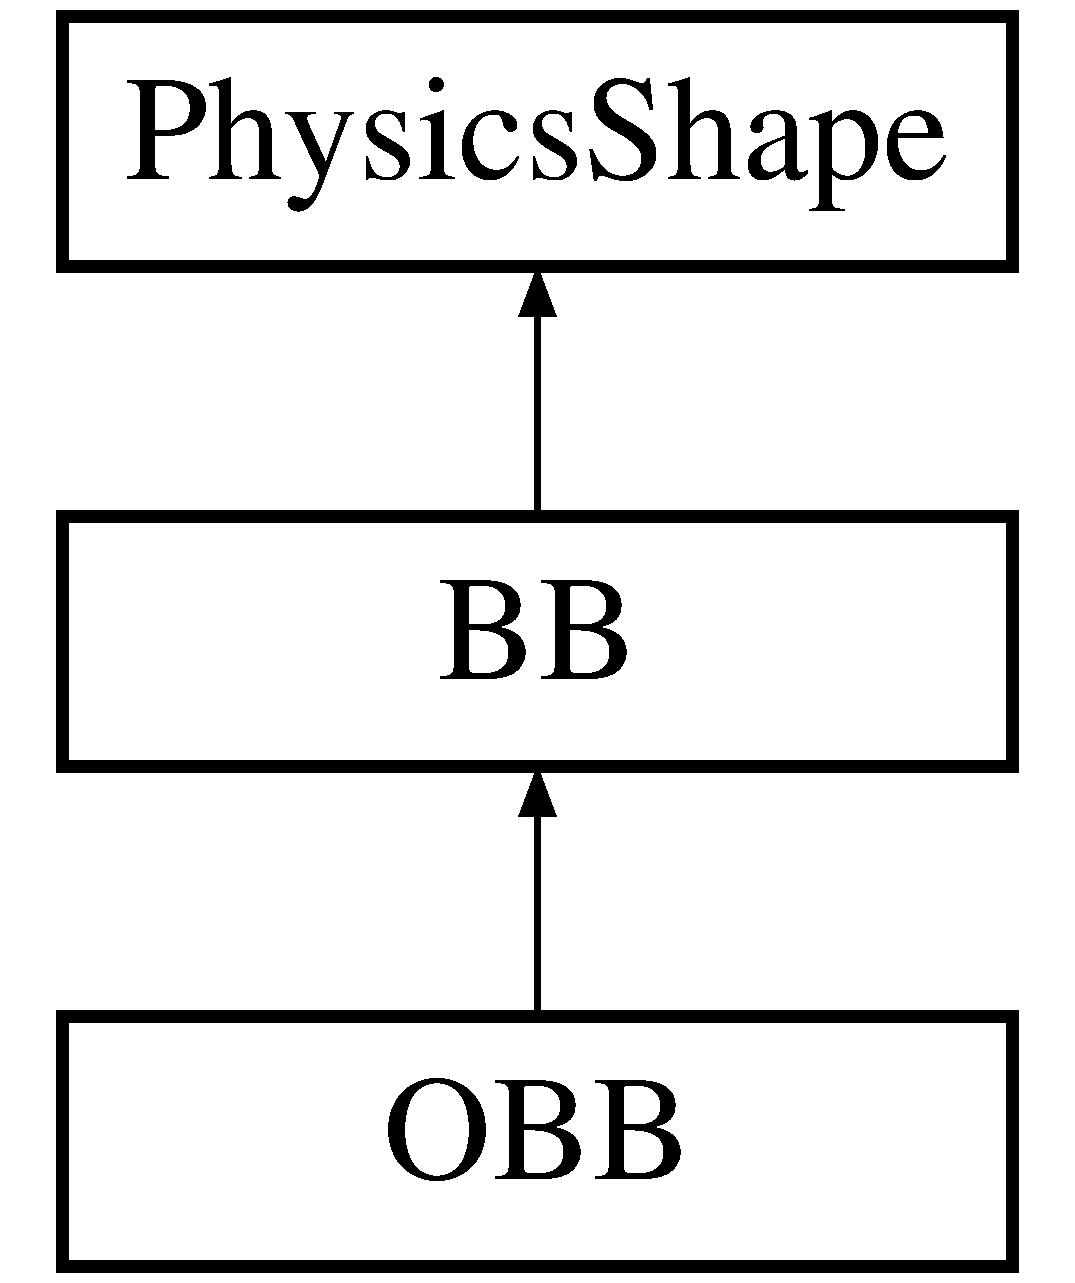
\includegraphics[height=3.000000cm]{class_o_b_b}
\end{center}
\end{figure}
\subsection*{Public Member Functions}
\begin{DoxyCompactItemize}
\item 
\hypertarget{class_o_b_b_a587dbcad47e99aa38ee6fc4168e710a5}{\hyperlink{class_o_b_b_a587dbcad47e99aa38ee6fc4168e710a5}{O\+B\+B} (const \hyperlink{class_vector2_d}{Vector2\+D}$<$ float $>$ \&k\+Half)}\label{class_o_b_b_a587dbcad47e99aa38ee6fc4168e710a5}

\begin{DoxyCompactList}\small\item\em Default Constructor. \end{DoxyCompactList}\item 
\hypertarget{class_o_b_b_a11ee7dd0ba7b814f63183a1b538de85a}{virtual float \hyperlink{class_o_b_b_a11ee7dd0ba7b814f63183a1b538de85a}{compute\+Inertia} (const float kf\+Mass) const }\label{class_o_b_b_a11ee7dd0ba7b814f63183a1b538de85a}

\begin{DoxyCompactList}\small\item\em Constructor which takes Half Extents. \end{DoxyCompactList}\item 
\hypertarget{class_o_b_b_adb59b9c3293c41afdb5646a7482ce181}{virtual float \hyperlink{class_o_b_b_adb59b9c3293c41afdb5646a7482ce181}{compute\+Area} () const }\label{class_o_b_b_adb59b9c3293c41afdb5646a7482ce181}

\begin{DoxyCompactList}\small\item\em Compute the moment of inertia of the shape. \end{DoxyCompactList}\end{DoxyCompactItemize}
\subsection*{Additional Inherited Members}


\subsection{Detailed Description}
an Orientated Bounding \hyperlink{class_box}{Box} which inherits from \hyperlink{class_b_b}{B\+B} 

The documentation for this class was generated from the following file\+:\begin{DoxyCompactItemize}
\item 
include/\hyperlink{_b_b_8h}{B\+B.\+h}\end{DoxyCompactItemize}

\hypertarget{class_orientated_box}{\section{Orientated\+Box Class Reference}
\label{class_orientated_box}\index{Orientated\+Box@{Orientated\+Box}}
}


an orientated physics body with a solid colour  




{\ttfamily \#include $<$Orientated\+Box.\+h$>$}

Inheritance diagram for Orientated\+Box\+:\begin{figure}[H]
\begin{center}
\leavevmode
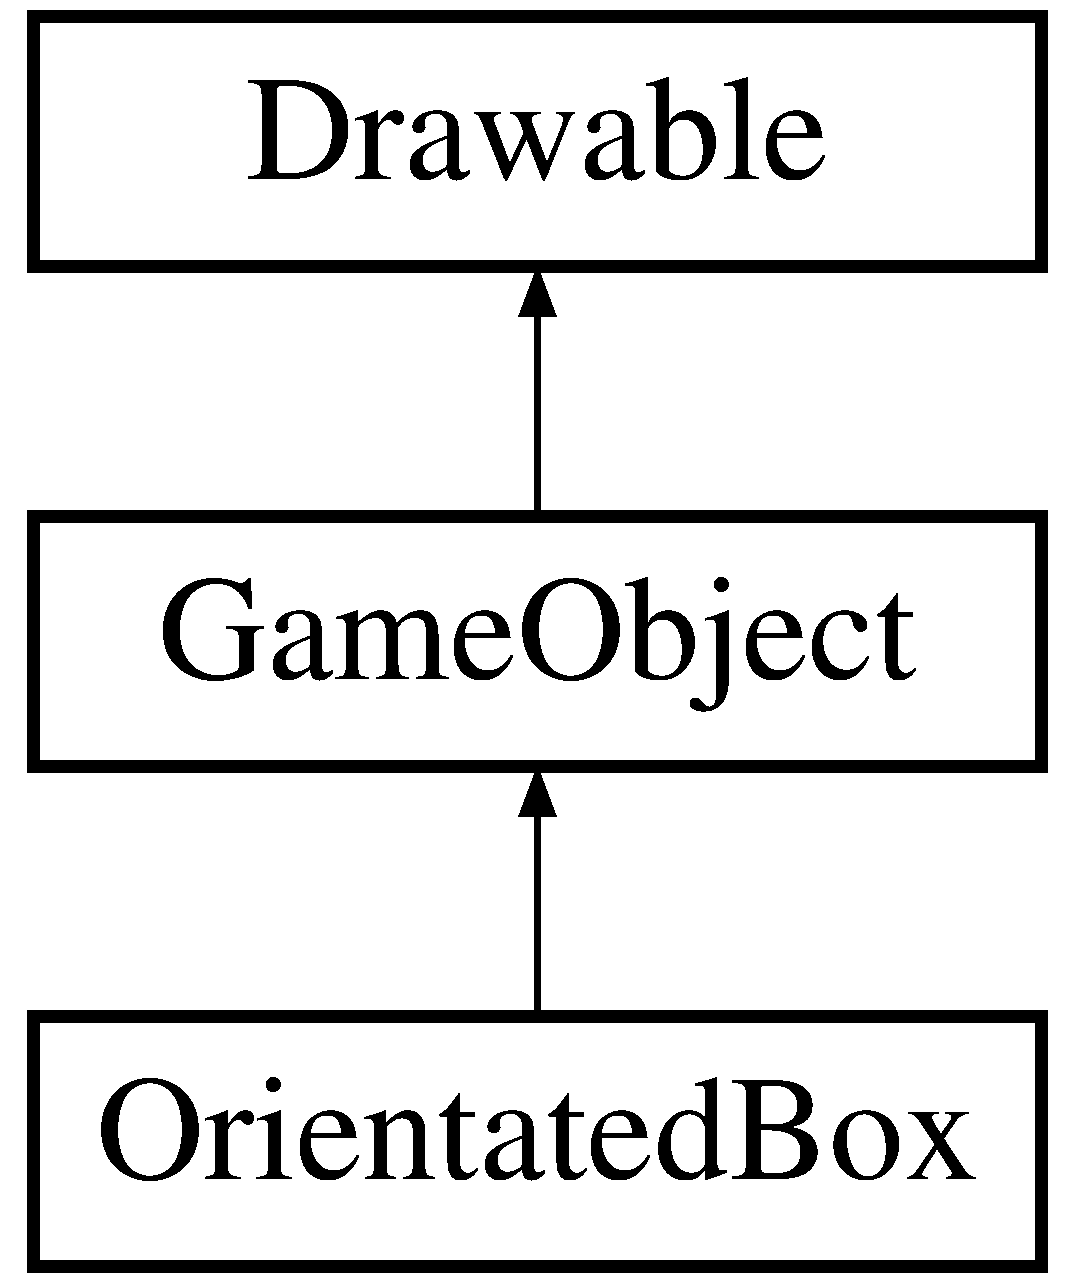
\includegraphics[height=3.000000cm]{class_orientated_box}
\end{center}
\end{figure}
\subsection*{Public Member Functions}
\begin{DoxyCompactItemize}
\item 
\hypertarget{class_orientated_box_a8ce9868a436dbbcd874d576dd25de2da}{\hyperlink{class_orientated_box_a8ce9868a436dbbcd874d576dd25de2da}{Orientated\+Box} ()}\label{class_orientated_box_a8ce9868a436dbbcd874d576dd25de2da}

\begin{DoxyCompactList}\small\item\em Default Constructor. \end{DoxyCompactList}\item 
\hypertarget{class_orientated_box_a9d33842f40fe272b541c4b95028da5ad}{{\bfseries Orientated\+Box} (const \hyperlink{class_vector2_d}{Vector2\+D}$<$ float $>$ \&k\+Pos, const \hyperlink{class_vector2_d}{Vector2\+D}$<$ float $>$ \&k\+Half\+Extents, const float kf\+Angle)}\label{class_orientated_box_a9d33842f40fe272b541c4b95028da5ad}

\item 
\hypertarget{class_orientated_box_ae1c39bcc43b31b0faf01c16dadc02d3b}{virtual void \hyperlink{class_orientated_box_ae1c39bcc43b31b0faf01c16dadc02d3b}{transform} ()}\label{class_orientated_box_ae1c39bcc43b31b0faf01c16dadc02d3b}

\begin{DoxyCompactList}\small\item\em Transform the graphics. \end{DoxyCompactList}\item 
virtual void \hyperlink{class_orientated_box_acf0c8800cd7024c9d346c33d299dc2cd}{draw} (sf\+::\+Render\+Target \&target, sf\+::\+Render\+States states) const 
\begin{DoxyCompactList}\small\item\em Draw the box. \end{DoxyCompactList}\item 
void \hyperlink{class_orientated_box_a8ddf109e746d64d0e40f7832b0d8533b}{set\+Colour} (const sf\+::\+Color \&col)
\begin{DoxyCompactList}\small\item\em Sets the colour of the box. \end{DoxyCompactList}\end{DoxyCompactItemize}
\subsection*{Public Attributes}
\begin{DoxyCompactItemize}
\item 
\hypertarget{class_orientated_box_a59080afaa1fc39741a7a540caaf64058}{std\+::shared\+\_\+ptr$<$ \hyperlink{class_body2_d}{Body2\+D} $>$ \hyperlink{class_orientated_box_a59080afaa1fc39741a7a540caaf64058}{g\+\_\+p\+Body}}\label{class_orientated_box_a59080afaa1fc39741a7a540caaf64058}

\begin{DoxyCompactList}\small\item\em Pointer to the physics body. \end{DoxyCompactList}\end{DoxyCompactItemize}
\subsection*{Additional Inherited Members}


\subsection{Detailed Description}
an orientated physics body with a solid colour 

\subsection{Member Function Documentation}
\hypertarget{class_orientated_box_acf0c8800cd7024c9d346c33d299dc2cd}{\index{Orientated\+Box@{Orientated\+Box}!draw@{draw}}
\index{draw@{draw}!Orientated\+Box@{Orientated\+Box}}
\subsubsection[{draw}]{\setlength{\rightskip}{0pt plus 5cm}void Orientated\+Box\+::draw (
\begin{DoxyParamCaption}
\item[{sf\+::\+Render\+Target \&}]{target, }
\item[{sf\+::\+Render\+States}]{states}
\end{DoxyParamCaption}
) const\hspace{0.3cm}{\ttfamily [virtual]}}}\label{class_orientated_box_acf0c8800cd7024c9d346c33d299dc2cd}


Draw the box. 

$<$ Draw the particle \hypertarget{class_orientated_box_a8ddf109e746d64d0e40f7832b0d8533b}{\index{Orientated\+Box@{Orientated\+Box}!set\+Colour@{set\+Colour}}
\index{set\+Colour@{set\+Colour}!Orientated\+Box@{Orientated\+Box}}
\subsubsection[{set\+Colour}]{\setlength{\rightskip}{0pt plus 5cm}void Orientated\+Box\+::set\+Colour (
\begin{DoxyParamCaption}
\item[{const sf\+::\+Color \&}]{col}
\end{DoxyParamCaption}
)}}\label{class_orientated_box_a8ddf109e746d64d0e40f7832b0d8533b}


Sets the colour of the box. 


\begin{DoxyParams}{Parameters}
{\em col} & new colour \\
\hline
\end{DoxyParams}


The documentation for this class was generated from the following files\+:\begin{DoxyCompactItemize}
\item 
include/Orientated\+Box.\+h\item 
src/Orientated\+Box.\+cpp\end{DoxyCompactItemize}

\hypertarget{struct_orientation_data}{\section{Orientation\+Data Struct Reference}
\label{struct_orientation_data}\index{Orientation\+Data@{Orientation\+Data}}
}


{\ttfamily \#include $<$Body2\+D.\+h$>$}

\subsection*{Public Attributes}
\begin{DoxyCompactItemize}
\item 
\hypertarget{struct_orientation_data_a9cb40c50a44caeaaa0aa3f29fa867c11}{float {\bfseries f\+Inv\+Inertia}}\label{struct_orientation_data_a9cb40c50a44caeaaa0aa3f29fa867c11}

\item 
\hypertarget{struct_orientation_data_a6c9041628d19999662eebcc8bcfeff34}{float \hyperlink{struct_orientation_data_a6c9041628d19999662eebcc8bcfeff34}{f\+Angular\+Velocity}}\label{struct_orientation_data_a6c9041628d19999662eebcc8bcfeff34}

\begin{DoxyCompactList}\small\item\em Float value of the angular velocity in degrees per second. \end{DoxyCompactList}\end{DoxyCompactItemize}


\subsection{Detailed Description}
structure which stores information about the orientation of the body 

The documentation for this struct was generated from the following file\+:\begin{DoxyCompactItemize}
\item 
include/\hyperlink{_body2_d_8h}{Body2\+D.\+h}\end{DoxyCompactItemize}

\hypertarget{class_paddle}{\section{Paddle Class Reference}
\label{class_paddle}\index{Paddle@{Paddle}}
}


a paddle with a physics body  




{\ttfamily \#include $<$Paddle.\+h$>$}

Inheritance diagram for Paddle\+:\begin{figure}[H]
\begin{center}
\leavevmode
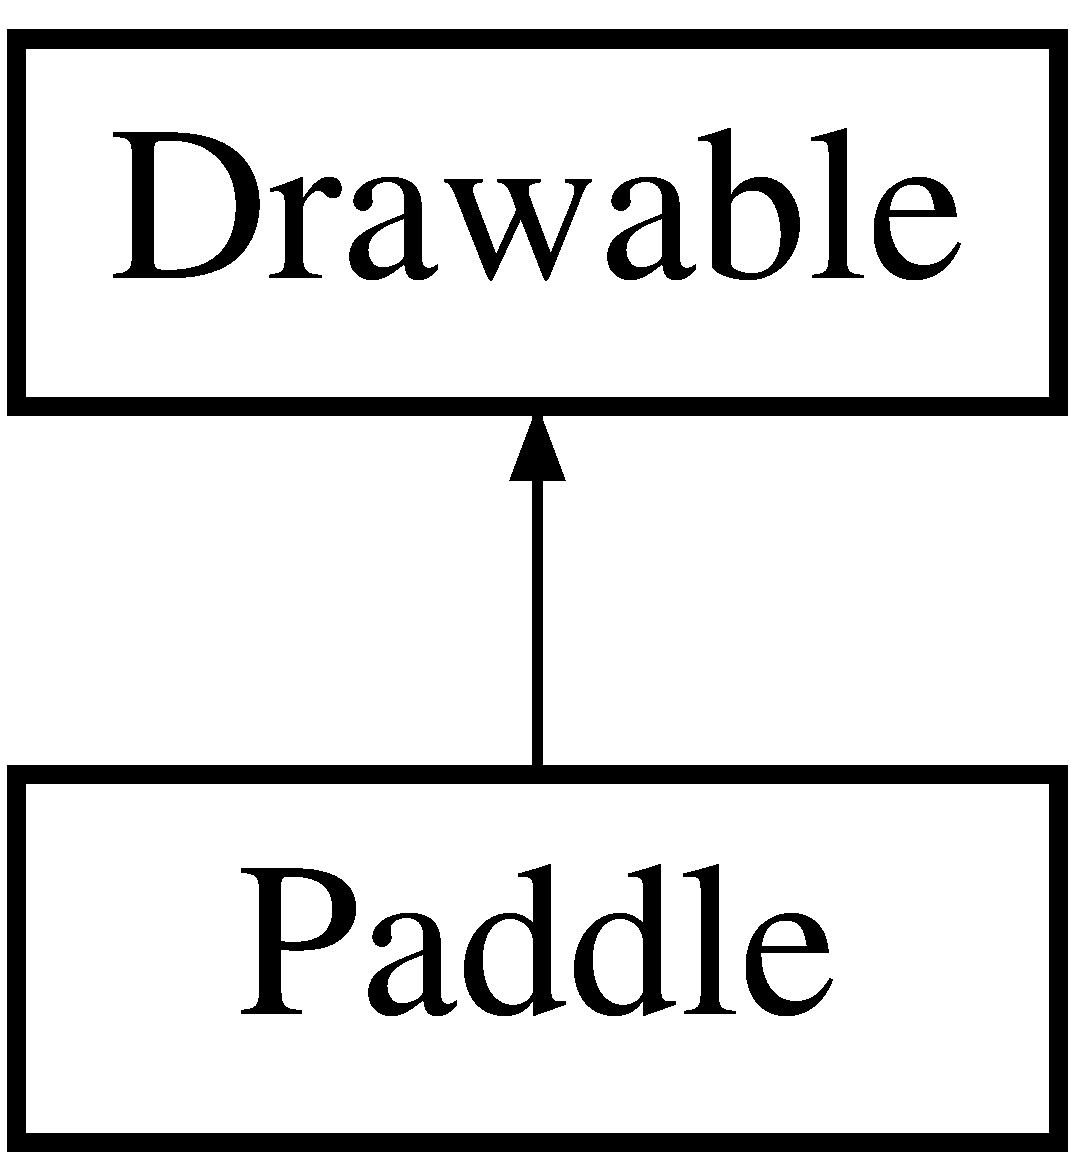
\includegraphics[height=2.000000cm]{class_paddle}
\end{center}
\end{figure}
\subsection*{Public Member Functions}
\begin{DoxyCompactItemize}
\item 
\hypertarget{class_paddle_a53895671ddfde9ba668546065ec4f164}{\hyperlink{class_paddle_a53895671ddfde9ba668546065ec4f164}{Paddle} ()}\label{class_paddle_a53895671ddfde9ba668546065ec4f164}

\begin{DoxyCompactList}\small\item\em Default constructor. \end{DoxyCompactList}\item 
\hypertarget{class_paddle_aa37bdcd24ceb267b5b2b7055c1002bb5}{{\bfseries Paddle} (const \hyperlink{class_vector2_d}{Vector2\+D}$<$ float $>$ \&k\+Pos, const \hyperlink{class_vector2_d}{Vector2\+D}$<$ float $>$ \&k\+Half\+Extents, const float kf\+Angle)}\label{class_paddle_aa37bdcd24ceb267b5b2b7055c1002bb5}

\item 
\hypertarget{class_paddle_a926ced17de3d812eddd5d6aa48118aba}{void \hyperlink{class_paddle_a926ced17de3d812eddd5d6aa48118aba}{set\+Left} ()}\label{class_paddle_a926ced17de3d812eddd5d6aa48118aba}

\begin{DoxyCompactList}\small\item\em Set as left paddle. \end{DoxyCompactList}\item 
\hypertarget{class_paddle_a21f17284347b540a210f669e46fb7033}{void \hyperlink{class_paddle_a21f17284347b540a210f669e46fb7033}{set\+Right} ()}\label{class_paddle_a21f17284347b540a210f669e46fb7033}

\begin{DoxyCompactList}\small\item\em Set as right paddle. \end{DoxyCompactList}\item 
\hypertarget{class_paddle_a9446a94c141d687ea3224fdba2dc7fa0}{void \hyperlink{class_paddle_a9446a94c141d687ea3224fdba2dc7fa0}{flip\+Up} ()}\label{class_paddle_a9446a94c141d687ea3224fdba2dc7fa0}

\begin{DoxyCompactList}\small\item\em Flip the paddle up. \end{DoxyCompactList}\item 
\hypertarget{class_paddle_a3bf356d44b28157c013240d3dde6f9d5}{void \hyperlink{class_paddle_a3bf356d44b28157c013240d3dde6f9d5}{flip\+Down} ()}\label{class_paddle_a3bf356d44b28157c013240d3dde6f9d5}

\begin{DoxyCompactList}\small\item\em Flip the paddle down. \end{DoxyCompactList}\item 
\hypertarget{class_paddle_a4e9ab8e3c5d087a8d23beed16f38dd00}{void \hyperlink{class_paddle_a4e9ab8e3c5d087a8d23beed16f38dd00}{transform} ()}\label{class_paddle_a4e9ab8e3c5d087a8d23beed16f38dd00}

\begin{DoxyCompactList}\small\item\em Transform the graphics. \end{DoxyCompactList}\item 
virtual void \hyperlink{class_paddle_a569a4a016b265cb3af3012061adafdea}{draw} (sf\+::\+Render\+Target \&target, sf\+::\+Render\+States states) const 
\begin{DoxyCompactList}\small\item\em Draw the paddle. \end{DoxyCompactList}\end{DoxyCompactItemize}
\subsection*{Public Attributes}
\begin{DoxyCompactItemize}
\item 
\hypertarget{class_paddle_aa1010d0654e87e6616bdc246f04d3ad6}{std\+::shared\+\_\+ptr$<$ \hyperlink{class_body2_d}{Body2\+D} $>$ \hyperlink{class_paddle_aa1010d0654e87e6616bdc246f04d3ad6}{g\+\_\+p\+Body}}\label{class_paddle_aa1010d0654e87e6616bdc246f04d3ad6}

\begin{DoxyCompactList}\small\item\em Pointer to the physics body. \end{DoxyCompactList}\end{DoxyCompactItemize}


\subsection{Detailed Description}
a paddle with a physics body 

\subsection{Member Function Documentation}
\hypertarget{class_paddle_a569a4a016b265cb3af3012061adafdea}{\index{Paddle@{Paddle}!draw@{draw}}
\index{draw@{draw}!Paddle@{Paddle}}
\subsubsection[{draw}]{\setlength{\rightskip}{0pt plus 5cm}void Paddle\+::draw (
\begin{DoxyParamCaption}
\item[{sf\+::\+Render\+Target \&}]{target, }
\item[{sf\+::\+Render\+States}]{states}
\end{DoxyParamCaption}
) const\hspace{0.3cm}{\ttfamily [virtual]}}}\label{class_paddle_a569a4a016b265cb3af3012061adafdea}


Draw the paddle. 

$<$ Draw the particle 

The documentation for this class was generated from the following files\+:\begin{DoxyCompactItemize}
\item 
include/\hyperlink{_paddle_8h}{Paddle.\+h}\item 
src/\hyperlink{_paddle_8cpp}{Paddle.\+cpp}\end{DoxyCompactItemize}

\hypertarget{class_pause_screen}{\section{Pause\+Screen Class Reference}
\label{class_pause_screen}\index{Pause\+Screen@{Pause\+Screen}}
}


a drawable which overlays on the screen when the gamee is paused or the game is over  




{\ttfamily \#include $<$Pause\+Screen.\+h$>$}

Inheritance diagram for Pause\+Screen\+:\begin{figure}[H]
\begin{center}
\leavevmode
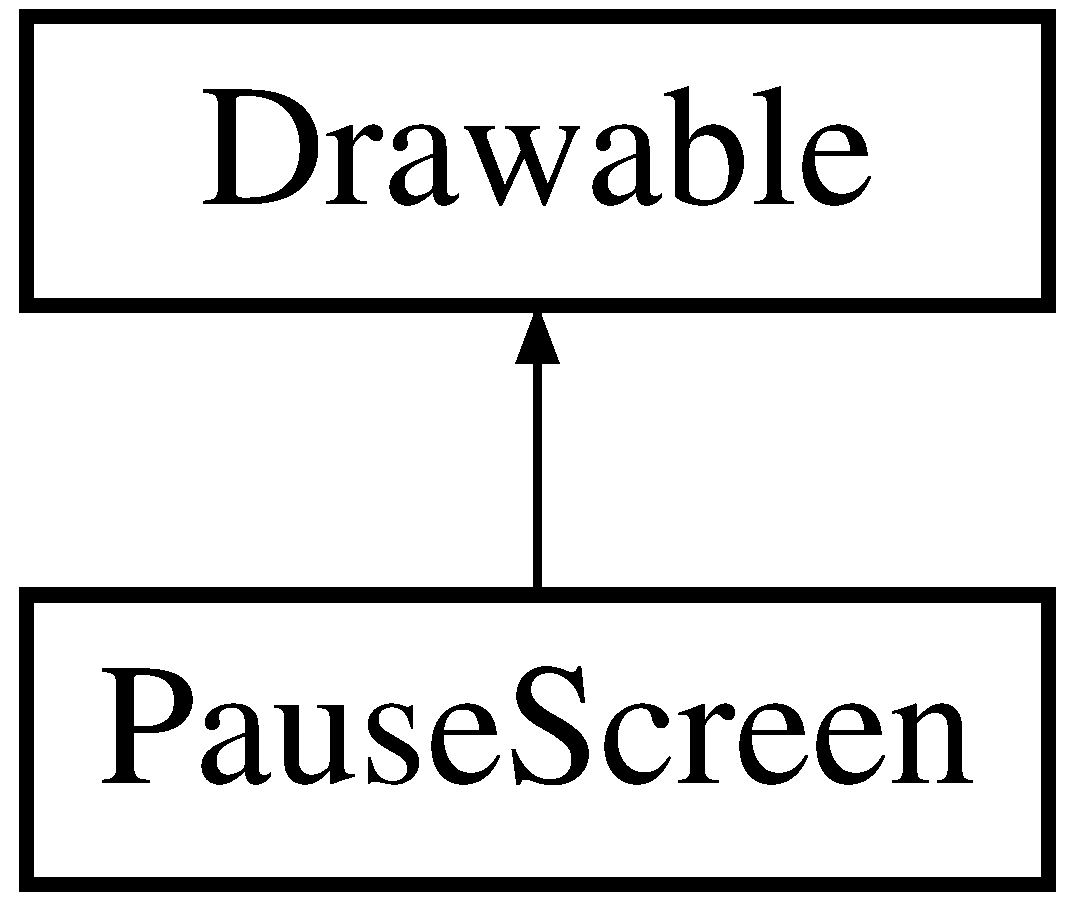
\includegraphics[height=2.000000cm]{class_pause_screen}
\end{center}
\end{figure}
\subsection*{Public Member Functions}
\begin{DoxyCompactItemize}
\item 
\hypertarget{class_pause_screen_a42a6d2150dbd1c523c374b04cb93c524}{\hyperlink{class_pause_screen_a42a6d2150dbd1c523c374b04cb93c524}{Pause\+Screen} ()}\label{class_pause_screen_a42a6d2150dbd1c523c374b04cb93c524}

\begin{DoxyCompactList}\small\item\em Default constructor. \end{DoxyCompactList}\item 
\hyperlink{class_pause_screen_a008433b17bf4da5799b76595395e2e0e}{Pause\+Screen} (sf\+::\+Font \&new\+Font)
\begin{DoxyCompactList}\small\item\em Constructor which takes a font. \end{DoxyCompactList}\item 
virtual void \hyperlink{class_pause_screen_a268c42dc11b1d8b6d5e141066e73d693}{draw} (sf\+::\+Render\+Target \&target, sf\+::\+Render\+States states) const 
\begin{DoxyCompactList}\small\item\em Draw the pause screen. \end{DoxyCompactList}\end{DoxyCompactItemize}


\subsection{Detailed Description}
a drawable which overlays on the screen when the gamee is paused or the game is over 

\subsection{Constructor \& Destructor Documentation}
\hypertarget{class_pause_screen_a008433b17bf4da5799b76595395e2e0e}{\index{Pause\+Screen@{Pause\+Screen}!Pause\+Screen@{Pause\+Screen}}
\index{Pause\+Screen@{Pause\+Screen}!Pause\+Screen@{Pause\+Screen}}
\subsubsection[{Pause\+Screen}]{\setlength{\rightskip}{0pt plus 5cm}Pause\+Screen\+::\+Pause\+Screen (
\begin{DoxyParamCaption}
\item[{sf\+::\+Font \&}]{new\+Font}
\end{DoxyParamCaption}
)}}\label{class_pause_screen_a008433b17bf4da5799b76595395e2e0e}


Constructor which takes a font. 


\begin{DoxyParams}{Parameters}
{\em new\+Font} & Constructor which takes a font \\
\hline
\end{DoxyParams}


\subsection{Member Function Documentation}
\hypertarget{class_pause_screen_a268c42dc11b1d8b6d5e141066e73d693}{\index{Pause\+Screen@{Pause\+Screen}!draw@{draw}}
\index{draw@{draw}!Pause\+Screen@{Pause\+Screen}}
\subsubsection[{draw}]{\setlength{\rightskip}{0pt plus 5cm}void Pause\+Screen\+::draw (
\begin{DoxyParamCaption}
\item[{sf\+::\+Render\+Target \&}]{target, }
\item[{sf\+::\+Render\+States}]{states}
\end{DoxyParamCaption}
) const\hspace{0.3cm}{\ttfamily [virtual]}}}\label{class_pause_screen_a268c42dc11b1d8b6d5e141066e73d693}


Draw the pause screen. 

$<$ Draw the pause screen 

The documentation for this class was generated from the following files\+:\begin{DoxyCompactItemize}
\item 
include/\hyperlink{_pause_screen_8h}{Pause\+Screen.\+h}\item 
src/\hyperlink{_pause_screen_8cpp}{Pause\+Screen.\+cpp}\end{DoxyCompactItemize}

\hypertarget{class_physics_shape}{\section{Physics\+Shape Class Reference}
\label{class_physics_shape}\index{Physics\+Shape@{Physics\+Shape}}
}


a 2\+D Physics Shape  




{\ttfamily \#include $<$Physics\+Shape.\+h$>$}

Inheritance diagram for Physics\+Shape\+:\begin{figure}[H]
\begin{center}
\leavevmode
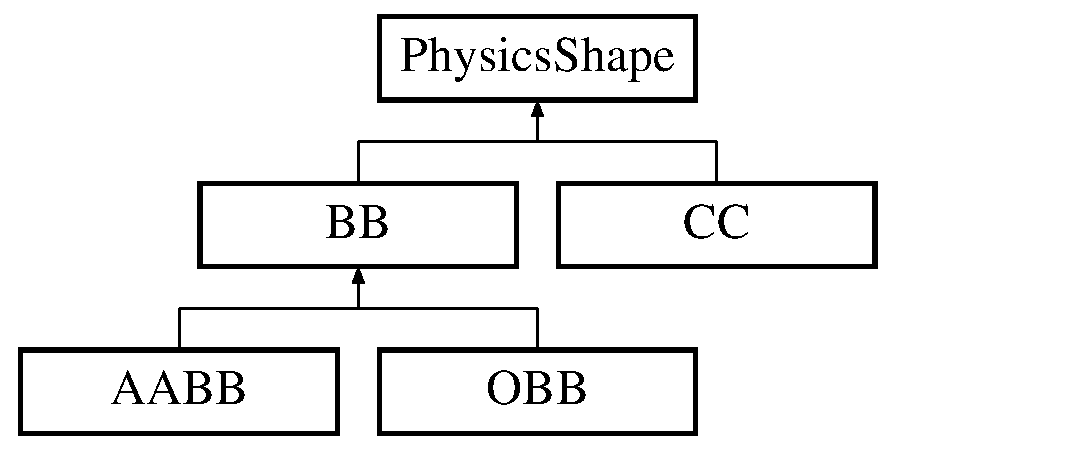
\includegraphics[height=3.000000cm]{class_physics_shape}
\end{center}
\end{figure}
\subsection*{Public Member Functions}
\begin{DoxyCompactItemize}
\item 
\hypertarget{class_physics_shape_af921c5335f89dd6c5e98bdceddb6b2c6}{\hyperlink{_physics_shape_8h_a20d894c0e61b699e6a53f0871418ea46}{body\+\_\+types} \hyperlink{class_physics_shape_af921c5335f89dd6c5e98bdceddb6b2c6}{get\+Body\+Type} () const }\label{class_physics_shape_af921c5335f89dd6c5e98bdceddb6b2c6}

\begin{DoxyCompactList}\small\item\em Default Constructor. \end{DoxyCompactList}\item 
\hypertarget{class_physics_shape_ae7bd37cc6d1c414e4d92649dba3cd791}{virtual float \hyperlink{class_physics_shape_ae7bd37cc6d1c414e4d92649dba3cd791}{compute\+Area} () const }\label{class_physics_shape_ae7bd37cc6d1c414e4d92649dba3cd791}

\begin{DoxyCompactList}\small\item\em Returns the type of physics shape. \end{DoxyCompactList}\item 
\hypertarget{class_physics_shape_a5e557a41a6dc5e77dfdf8e79a3d816d6}{virtual float \hyperlink{class_physics_shape_a5e557a41a6dc5e77dfdf8e79a3d816d6}{compute\+Inertia} (const float f\+\_\+\+Mass) const }\label{class_physics_shape_a5e557a41a6dc5e77dfdf8e79a3d816d6}

\begin{DoxyCompactList}\small\item\em Virtual function to compute the area of the shape. \end{DoxyCompactList}\end{DoxyCompactItemize}
\subsection*{Protected Attributes}
\begin{DoxyCompactItemize}
\item 
\hypertarget{class_physics_shape_aa22ced89280991e3466292624a2c16a4}{\hyperlink{_physics_shape_8h_a20d894c0e61b699e6a53f0871418ea46}{body\+\_\+types} \hyperlink{class_physics_shape_aa22ced89280991e3466292624a2c16a4}{m\+\_\+\+Body\+Type}}\label{class_physics_shape_aa22ced89280991e3466292624a2c16a4}

\begin{DoxyCompactList}\small\item\em Type of physics shape (to be set by sub-\/class) \end{DoxyCompactList}\end{DoxyCompactItemize}


\subsection{Detailed Description}
a 2\+D Physics Shape 

The documentation for this class was generated from the following file\+:\begin{DoxyCompactItemize}
\item 
include/\hyperlink{_physics_shape_8h}{Physics\+Shape.\+h}\end{DoxyCompactItemize}

\hypertarget{class_physics_sprite}{\section{Physics\+Sprite Class Reference}
\label{class_physics_sprite}\index{Physics\+Sprite@{Physics\+Sprite}}
}


A drawable physics object.  




{\ttfamily \#include $<$Physics\+Sprite.\+h$>$}

Inheritance diagram for Physics\+Sprite\+:\begin{figure}[H]
\begin{center}
\leavevmode
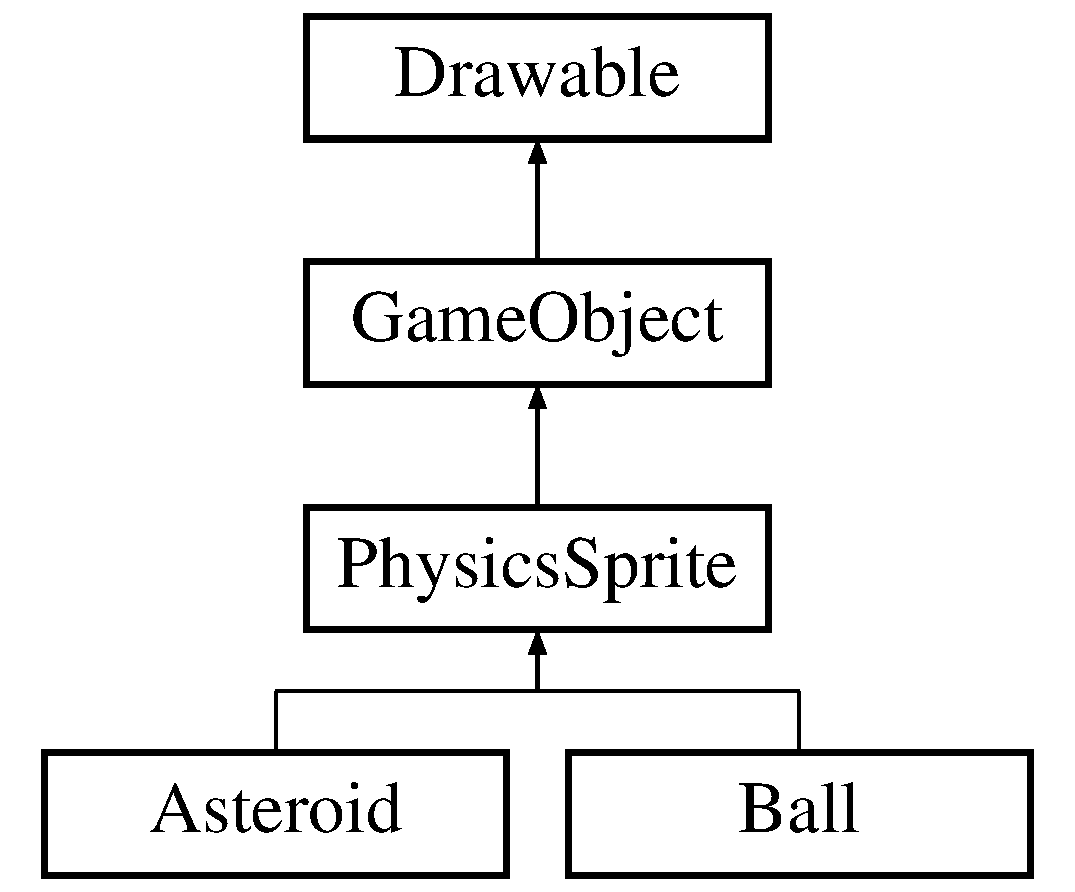
\includegraphics[height=4.000000cm]{class_physics_sprite}
\end{center}
\end{figure}
\subsection*{Public Member Functions}
\begin{DoxyCompactItemize}
\item 
\hypertarget{class_physics_sprite_a811ffe62810312784c4e632b54fadcdd}{\hyperlink{class_physics_sprite_a811ffe62810312784c4e632b54fadcdd}{Physics\+Sprite} ()}\label{class_physics_sprite_a811ffe62810312784c4e632b54fadcdd}

\begin{DoxyCompactList}\small\item\em Default constructor. \end{DoxyCompactList}\item 
void \hyperlink{class_physics_sprite_a5bceac4964f6995180af4ed21fcd1ae5}{set\+Texture} (const sf\+::\+Texture \&tex)
\begin{DoxyCompactList}\small\item\em Sets the texture of the sprite. \end{DoxyCompactList}\item 
\hypertarget{class_physics_sprite_a97720abd69161c946b159d2e5e7fca36}{virtual void \hyperlink{class_physics_sprite_a97720abd69161c946b159d2e5e7fca36}{transform} ()}\label{class_physics_sprite_a97720abd69161c946b159d2e5e7fca36}

\begin{DoxyCompactList}\small\item\em Transform the sprite. \end{DoxyCompactList}\item 
virtual void \hyperlink{class_physics_sprite_a96d93c233739c0b4ec3bce383db4b84f}{draw} (sf\+::\+Render\+Target \&target, sf\+::\+Render\+States states) const 
\begin{DoxyCompactList}\small\item\em Draw the physics sprite. \end{DoxyCompactList}\end{DoxyCompactItemize}
\subsection*{Public Attributes}
\begin{DoxyCompactItemize}
\item 
\hypertarget{class_physics_sprite_a763f9c183b5ddd1ea41992e011738792}{std\+::shared\+\_\+ptr$<$ \hyperlink{class_body2_d}{Body2\+D} $>$ \hyperlink{class_physics_sprite_a763f9c183b5ddd1ea41992e011738792}{g\+\_\+p\+Body}}\label{class_physics_sprite_a763f9c183b5ddd1ea41992e011738792}

\begin{DoxyCompactList}\small\item\em Pointer to the physics body. \end{DoxyCompactList}\end{DoxyCompactItemize}
\subsection*{Protected Attributes}
\begin{DoxyCompactItemize}
\item 
\hypertarget{class_physics_sprite_a307206e2e32121fba9c35a0ff5156bf0}{sf\+::\+Texture \hyperlink{class_physics_sprite_a307206e2e32121fba9c35a0ff5156bf0}{m\+\_\+texture}}\label{class_physics_sprite_a307206e2e32121fba9c35a0ff5156bf0}

\begin{DoxyCompactList}\small\item\em Sprite texture. \end{DoxyCompactList}\item 
\hypertarget{class_physics_sprite_a956c25d8bd5b34f697cc33eedc4f5aba}{sf\+::\+Sprite \hyperlink{class_physics_sprite_a956c25d8bd5b34f697cc33eedc4f5aba}{m\+\_\+sprite}}\label{class_physics_sprite_a956c25d8bd5b34f697cc33eedc4f5aba}

\begin{DoxyCompactList}\small\item\em Sprite. \end{DoxyCompactList}\end{DoxyCompactItemize}


\subsection{Detailed Description}
A drawable physics object. 

\subsection{Member Function Documentation}
\hypertarget{class_physics_sprite_a96d93c233739c0b4ec3bce383db4b84f}{\index{Physics\+Sprite@{Physics\+Sprite}!draw@{draw}}
\index{draw@{draw}!Physics\+Sprite@{Physics\+Sprite}}
\subsubsection[{draw}]{\setlength{\rightskip}{0pt plus 5cm}void Physics\+Sprite\+::draw (
\begin{DoxyParamCaption}
\item[{sf\+::\+Render\+Target \&}]{target, }
\item[{sf\+::\+Render\+States}]{states}
\end{DoxyParamCaption}
) const\hspace{0.3cm}{\ttfamily [virtual]}}}\label{class_physics_sprite_a96d93c233739c0b4ec3bce383db4b84f}


Draw the physics sprite. 

$<$ Draw the physics sprite \hypertarget{class_physics_sprite_a5bceac4964f6995180af4ed21fcd1ae5}{\index{Physics\+Sprite@{Physics\+Sprite}!set\+Texture@{set\+Texture}}
\index{set\+Texture@{set\+Texture}!Physics\+Sprite@{Physics\+Sprite}}
\subsubsection[{set\+Texture}]{\setlength{\rightskip}{0pt plus 5cm}void Physics\+Sprite\+::set\+Texture (
\begin{DoxyParamCaption}
\item[{const sf\+::\+Texture \&}]{tex}
\end{DoxyParamCaption}
)}}\label{class_physics_sprite_a5bceac4964f6995180af4ed21fcd1ae5}


Sets the texture of the sprite. 


\begin{DoxyParams}{Parameters}
{\em tex} & New texture \\
\hline
\end{DoxyParams}


The documentation for this class was generated from the following files\+:\begin{DoxyCompactItemize}
\item 
include/\hyperlink{_physics_sprite_8h}{Physics\+Sprite.\+h}\item 
src/\hyperlink{_physics_sprite_8cpp}{Physics\+Sprite.\+cpp}\end{DoxyCompactItemize}

\hypertarget{class_pinball_scene}{\section{Pinball\+Scene Class Reference}
\label{class_pinball_scene}\index{Pinball\+Scene@{Pinball\+Scene}}
}


a class which manages game logic and stores game objects, inherits from the \hyperlink{class_game_scene}{Game\+Scene} class  




{\ttfamily \#include $<$Pinball\+Scene.\+h$>$}

Inheritance diagram for Pinball\+Scene\+:\begin{figure}[H]
\begin{center}
\leavevmode
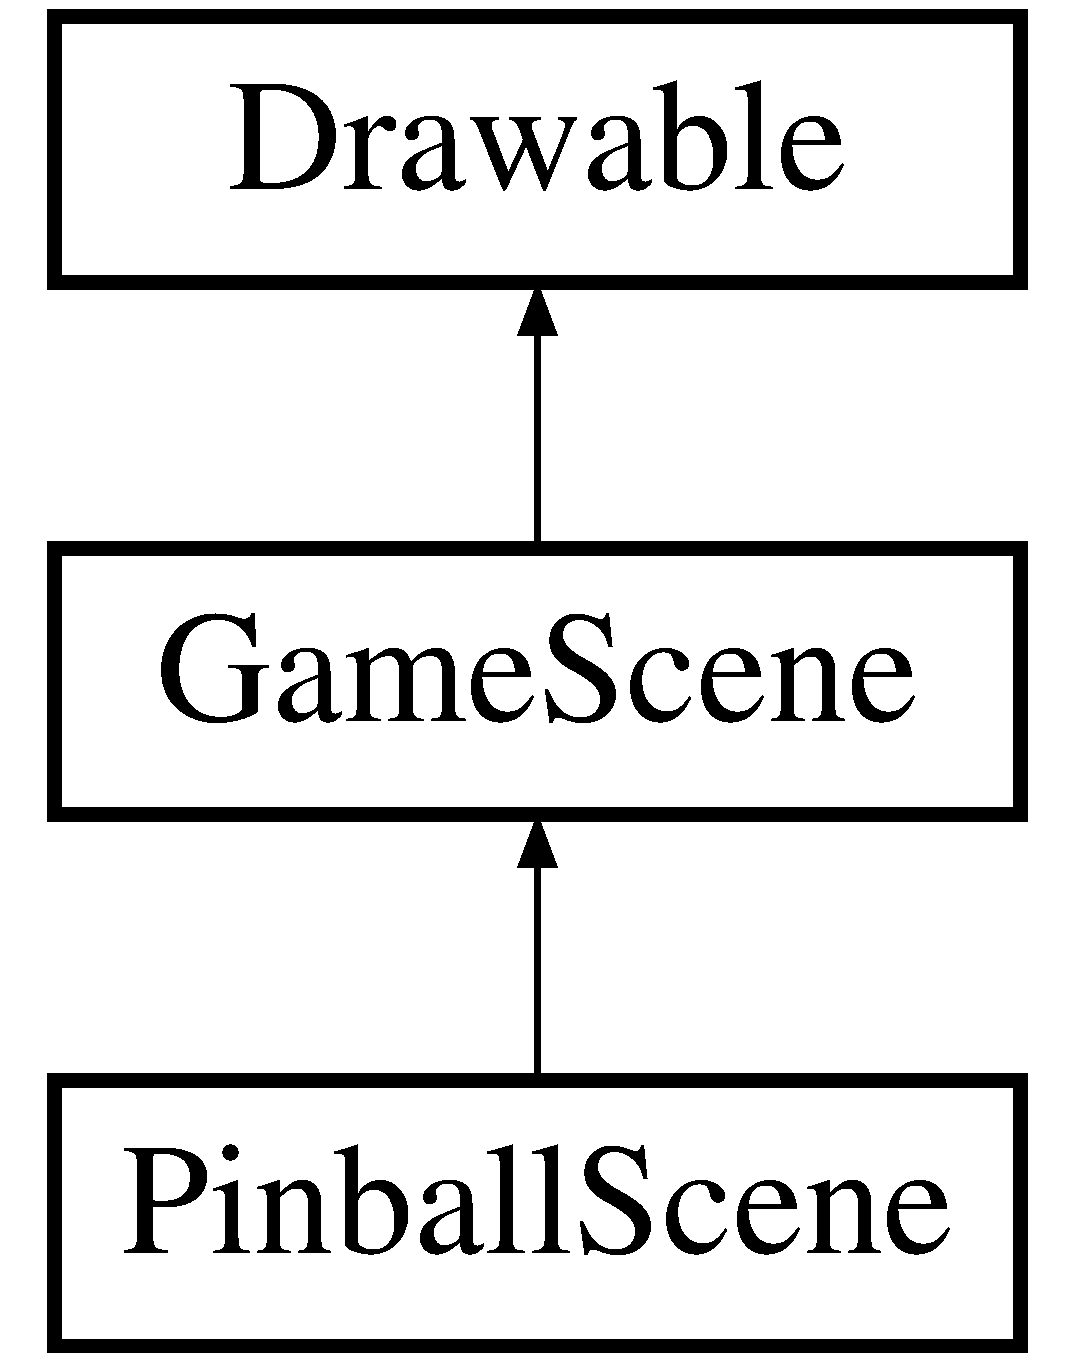
\includegraphics[height=3.000000cm]{class_pinball_scene}
\end{center}
\end{figure}
\subsection*{Public Member Functions}
\begin{DoxyCompactItemize}
\item 
\hypertarget{class_pinball_scene_af6b0e0d7d9765249018dacccc9b4c681}{\hyperlink{class_pinball_scene_af6b0e0d7d9765249018dacccc9b4c681}{Pinball\+Scene} ()}\label{class_pinball_scene_af6b0e0d7d9765249018dacccc9b4c681}

\begin{DoxyCompactList}\small\item\em Default Constructor. \end{DoxyCompactList}\item 
\hypertarget{class_pinball_scene_a99056b13a1d355643b5e2284decc659b}{virtual void \hyperlink{class_pinball_scene_a99056b13a1d355643b5e2284decc659b}{update} ()}\label{class_pinball_scene_a99056b13a1d355643b5e2284decc659b}

\begin{DoxyCompactList}\small\item\em Updates the game logic by the intveral. \end{DoxyCompactList}\item 
virtual void \hyperlink{class_pinball_scene_a57947a5d74f53f73a40df59de2c72078}{event} (sf\+::\+Event event)
\begin{DoxyCompactList}\small\item\em Called when an S\+F\+M\+L event occurs passing the event variable. \end{DoxyCompactList}\item 
virtual void \hyperlink{class_pinball_scene_adb8babf412aa47981951e55bacf66b03}{draw} (sf\+::\+Render\+Target \&target, sf\+::\+Render\+States states) const 
\begin{DoxyCompactList}\small\item\em Draw the scene. \end{DoxyCompactList}\end{DoxyCompactItemize}
\subsection*{Protected Member Functions}
\begin{DoxyCompactItemize}
\item 
\hypertarget{class_pinball_scene_ac42acaaab8d70b460aa8ed721951f951}{void \hyperlink{class_pinball_scene_ac42acaaab8d70b460aa8ed721951f951}{spawn\+New\+Ball} ()}\label{class_pinball_scene_ac42acaaab8d70b460aa8ed721951f951}

\begin{DoxyCompactList}\small\item\em Spawn a new ball. \end{DoxyCompactList}\item 
\hypertarget{class_pinball_scene_ace817bd823f2382a604d26f3447df3a2}{void \hyperlink{class_pinball_scene_ace817bd823f2382a604d26f3447df3a2}{restart\+Game} ()}\label{class_pinball_scene_ace817bd823f2382a604d26f3447df3a2}

\begin{DoxyCompactList}\small\item\em Restart the game. \end{DoxyCompactList}\item 
\hypertarget{class_pinball_scene_a8d760114d715152b057be9ea678e95bf}{void \hyperlink{class_pinball_scene_a8d760114d715152b057be9ea678e95bf}{setup\+Objects} ()}\label{class_pinball_scene_a8d760114d715152b057be9ea678e95bf}

\begin{DoxyCompactList}\small\item\em sets up the objects in the scene \end{DoxyCompactList}\end{DoxyCompactItemize}
\subsection*{Protected Attributes}
\begin{DoxyCompactItemize}
\item 
\hypertarget{class_pinball_scene_a33388520907fb2e994252aab123487cc}{\hyperlink{_game_config_8h_a7899b65f1ea0f655e4bbf8d2a5714285}{Game\+State} \hyperlink{class_pinball_scene_a33388520907fb2e994252aab123487cc}{m\+\_\+\+Game\+State}}\label{class_pinball_scene_a33388520907fb2e994252aab123487cc}

\begin{DoxyCompactList}\small\item\em Current game state. \end{DoxyCompactList}\item 
\hypertarget{class_pinball_scene_a620a2dbb8448ff4b9ed9b470e9d0faaa}{\hyperlink{class_sprite_manager}{Sprite\+Manager} \hyperlink{class_pinball_scene_a620a2dbb8448ff4b9ed9b470e9d0faaa}{m\+\_\+\+Sprite\+Manager}}\label{class_pinball_scene_a620a2dbb8448ff4b9ed9b470e9d0faaa}

\begin{DoxyCompactList}\small\item\em Sprite manager for loading textures. \end{DoxyCompactList}\item 
\hypertarget{class_pinball_scene_aec50641fc82974b3edf02d1956098374}{std\+::shared\+\_\+ptr$<$ \hyperlink{class_u_i_manager}{U\+I\+Manager} $>$ \hyperlink{class_pinball_scene_aec50641fc82974b3edf02d1956098374}{m\+\_\+p\+Ui\+Manager}}\label{class_pinball_scene_aec50641fc82974b3edf02d1956098374}

\begin{DoxyCompactList}\small\item\em Pointer to the points manager. \end{DoxyCompactList}\item 
\hypertarget{class_pinball_scene_a0404c72469c589e6b93c38cfb31c747d}{\hyperlink{class_asteroid_field}{Asteroid\+Field} \hyperlink{class_pinball_scene_a0404c72469c589e6b93c38cfb31c747d}{m\+\_\+\+Asteroid\+Field}}\label{class_pinball_scene_a0404c72469c589e6b93c38cfb31c747d}

\begin{DoxyCompactList}\small\item\em Field of asteroids. \end{DoxyCompactList}\item 
\hypertarget{class_pinball_scene_a01c03b087726619b98865047f25e7476}{std\+::shared\+\_\+ptr$<$ \hyperlink{class_ball}{Ball} $>$ \hyperlink{class_pinball_scene_a01c03b087726619b98865047f25e7476}{m\+\_\+p\+Ball}}\label{class_pinball_scene_a01c03b087726619b98865047f25e7476}

\begin{DoxyCompactList}\small\item\em the player ball \end{DoxyCompactList}\item 
\hypertarget{class_pinball_scene_ae9b2a7e5fe0e0334ac2e4a5238f8fe3f}{std\+::shared\+\_\+ptr$<$ \hyperlink{class_ball}{Ball} $>$ \hyperlink{class_pinball_scene_ae9b2a7e5fe0e0334ac2e4a5238f8fe3f}{m\+\_\+p\+Black\+Hole}}\label{class_pinball_scene_ae9b2a7e5fe0e0334ac2e4a5238f8fe3f}

\begin{DoxyCompactList}\small\item\em Blackhole. \end{DoxyCompactList}\item 
\hypertarget{class_pinball_scene_a82759060543078ac218315d2a13618c1}{std\+::vector$<$ std\+::shared\+\_\+ptr\\*
$<$ \hyperlink{class_orientated_box}{Orientated\+Box} $>$ $>$ \hyperlink{class_pinball_scene_a82759060543078ac218315d2a13618c1}{m\+\_\+p\+Boxes}}\label{class_pinball_scene_a82759060543078ac218315d2a13618c1}

\begin{DoxyCompactList}\small\item\em Vector of orientated box. \end{DoxyCompactList}\item 
\hypertarget{class_pinball_scene_a56a94580b385ae849a4f9e90632e6ba0}{std\+::vector$<$ std\+::shared\+\_\+ptr\\*
$<$ \hyperlink{class_box}{Box} $>$ $>$ \hyperlink{class_pinball_scene_a56a94580b385ae849a4f9e90632e6ba0}{m\+\_\+p\+Walls}}\label{class_pinball_scene_a56a94580b385ae849a4f9e90632e6ba0}

\begin{DoxyCompactList}\small\item\em Vector of non-\/orientated boxes. \end{DoxyCompactList}\item 
\hypertarget{class_pinball_scene_a01f8eaffbfe7ba7f83f26006400a5e5c}{std\+::vector$<$ std\+::shared\+\_\+ptr\\*
$<$ \hyperlink{class_circular_bumper}{Circular\+Bumper} $>$ $>$ \hyperlink{class_pinball_scene_a01f8eaffbfe7ba7f83f26006400a5e5c}{m\+\_\+p\+Bumpers}}\label{class_pinball_scene_a01f8eaffbfe7ba7f83f26006400a5e5c}

\begin{DoxyCompactList}\small\item\em Vector of circular bumpers. \end{DoxyCompactList}\item 
\hypertarget{class_pinball_scene_a1e5a61e23b78a270ce4ae4abecc4c85a}{sf\+::\+Texture \hyperlink{class_pinball_scene_a1e5a61e23b78a270ce4ae4abecc4c85a}{m\+\_\+\+Background\+Texture}}\label{class_pinball_scene_a1e5a61e23b78a270ce4ae4abecc4c85a}

\begin{DoxyCompactList}\small\item\em Texture of the background. \end{DoxyCompactList}\item 
\hypertarget{class_pinball_scene_a6c8d33874806f5c0cbc02fefd9aab5ba}{sf\+::\+Sprite \hyperlink{class_pinball_scene_a6c8d33874806f5c0cbc02fefd9aab5ba}{m\+\_\+\+Background\+Sprite}}\label{class_pinball_scene_a6c8d33874806f5c0cbc02fefd9aab5ba}

\begin{DoxyCompactList}\small\item\em Sprite of. \end{DoxyCompactList}\item 
\hypertarget{class_pinball_scene_a77725348869b92b1340bc31313d46911}{\hyperlink{class_pause_screen}{Pause\+Screen} \hyperlink{class_pinball_scene_a77725348869b92b1340bc31313d46911}{m\+\_\+\+Pause\+Screen}}\label{class_pinball_scene_a77725348869b92b1340bc31313d46911}

\begin{DoxyCompactList}\small\item\em Games pause screen. \end{DoxyCompactList}\item 
\hypertarget{class_pinball_scene_a825899b11e3635e68d4473f0e1b96966}{\hyperlink{class_paddle}{Paddle} \hyperlink{class_pinball_scene_a825899b11e3635e68d4473f0e1b96966}{m\+\_\+\+Paddle\+Left}}\label{class_pinball_scene_a825899b11e3635e68d4473f0e1b96966}

\begin{DoxyCompactList}\small\item\em Left paddle. \end{DoxyCompactList}\item 
\hypertarget{class_pinball_scene_a2e32a793cac4b9c7aa64f3541acf71ed}{\hyperlink{class_paddle}{Paddle} \hyperlink{class_pinball_scene_a2e32a793cac4b9c7aa64f3541acf71ed}{m\+\_\+\+Paddle\+Right}}\label{class_pinball_scene_a2e32a793cac4b9c7aa64f3541acf71ed}

\begin{DoxyCompactList}\small\item\em Right paddle. \end{DoxyCompactList}\item 
\hypertarget{class_pinball_scene_ab19b6433abc3043db72f8bc11c75b2d3}{\hyperlink{class_spring}{Spring} \hyperlink{class_pinball_scene_ab19b6433abc3043db72f8bc11c75b2d3}{m\+\_\+\+Spring}}\label{class_pinball_scene_ab19b6433abc3043db72f8bc11c75b2d3}

\begin{DoxyCompactList}\small\item\em \hyperlink{class_spring}{Spring} (ball launcher) \end{DoxyCompactList}\end{DoxyCompactItemize}


\subsection{Detailed Description}
a class which manages game logic and stores game objects, inherits from the \hyperlink{class_game_scene}{Game\+Scene} class 

\subsection{Member Function Documentation}
\hypertarget{class_pinball_scene_adb8babf412aa47981951e55bacf66b03}{\index{Pinball\+Scene@{Pinball\+Scene}!draw@{draw}}
\index{draw@{draw}!Pinball\+Scene@{Pinball\+Scene}}
\subsubsection[{draw}]{\setlength{\rightskip}{0pt plus 5cm}void Pinball\+Scene\+::draw (
\begin{DoxyParamCaption}
\item[{sf\+::\+Render\+Target \&}]{target, }
\item[{sf\+::\+Render\+States}]{states}
\end{DoxyParamCaption}
) const\hspace{0.3cm}{\ttfamily [virtual]}}}\label{class_pinball_scene_adb8babf412aa47981951e55bacf66b03}


Draw the scene. 

$<$ Draw the scene 

Reimplemented from \hyperlink{class_game_scene}{Game\+Scene}.

\hypertarget{class_pinball_scene_a57947a5d74f53f73a40df59de2c72078}{\index{Pinball\+Scene@{Pinball\+Scene}!event@{event}}
\index{event@{event}!Pinball\+Scene@{Pinball\+Scene}}
\subsubsection[{event}]{\setlength{\rightskip}{0pt plus 5cm}void Pinball\+Scene\+::event (
\begin{DoxyParamCaption}
\item[{sf\+::\+Event}]{event}
\end{DoxyParamCaption}
)\hspace{0.3cm}{\ttfamily [virtual]}}}\label{class_pinball_scene_a57947a5d74f53f73a40df59de2c72078}


Called when an S\+F\+M\+L event occurs passing the event variable. 


\begin{DoxyParams}{Parameters}
{\em event} & S\+F\+M\+L event \\
\hline
\end{DoxyParams}


Reimplemented from \hyperlink{class_game_scene_a9cf68fbf8e0805cbb1618a71e04d7fa4}{Game\+Scene}.



The documentation for this class was generated from the following files\+:\begin{DoxyCompactItemize}
\item 
include/\hyperlink{_pinball_scene_8h}{Pinball\+Scene.\+h}\item 
src/\hyperlink{_pinball_scene_8cpp}{Pinball\+Scene.\+cpp}\end{DoxyCompactItemize}

\hypertarget{class_points_collider}{\section{Points\+Collider Class Reference}
\label{class_points_collider}\index{Points\+Collider@{Points\+Collider}}
}


a class which inherits from the \hyperlink{class_body2_d}{Body2\+D} class and adds points to the player score when hit  




{\ttfamily \#include $<$Points\+Collider.\+h$>$}

Inheritance diagram for Points\+Collider\+:\begin{figure}[H]
\begin{center}
\leavevmode
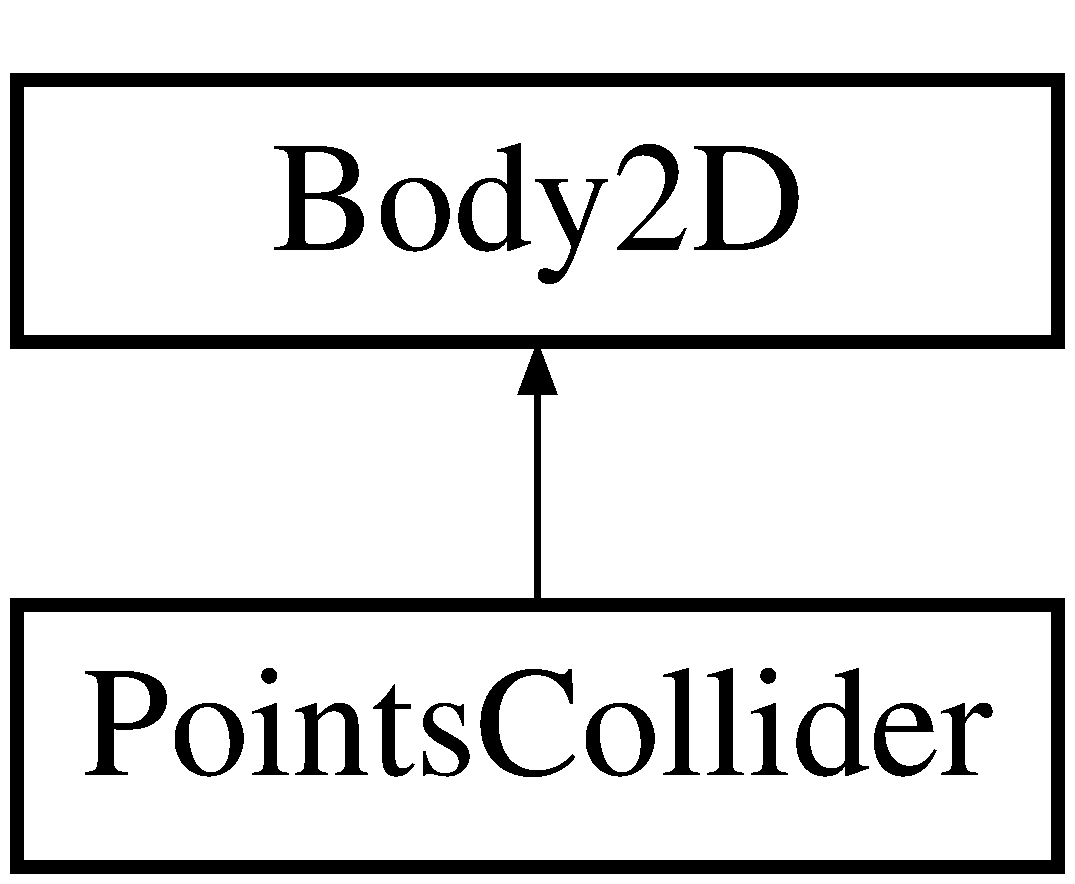
\includegraphics[height=2.000000cm]{class_points_collider}
\end{center}
\end{figure}
\subsection*{Public Member Functions}
\begin{DoxyCompactItemize}
\item 
\hyperlink{class_points_collider_ad51a37d4026b09b8efef51e0098602aa}{Points\+Collider} (const std\+::shared\+\_\+ptr$<$ \hyperlink{class_physics_shape}{Physics\+Shape} $>$ kp\+Physics\+Shape, const int ki\+Collide\+Value, const std\+::shared\+\_\+ptr$<$ \hyperlink{class_u_i_manager}{U\+I\+Manager} $>$ kp\+Manager)
\item 
virtual void \hyperlink{class_points_collider_ad24d2f1ba11e34a52e9caef300239de6}{collided} (const std\+::shared\+\_\+ptr$<$ \hyperlink{class_body2_d}{Body2\+D} $>$ \&kp\+Body)
\begin{DoxyCompactList}\small\item\em A Method called when the body collides with another body. \end{DoxyCompactList}\end{DoxyCompactItemize}
\subsection*{Additional Inherited Members}


\subsection{Detailed Description}
a class which inherits from the \hyperlink{class_body2_d}{Body2\+D} class and adds points to the player score when hit 

\subsection{Constructor \& Destructor Documentation}
\hypertarget{class_points_collider_ad51a37d4026b09b8efef51e0098602aa}{\index{Points\+Collider@{Points\+Collider}!Points\+Collider@{Points\+Collider}}
\index{Points\+Collider@{Points\+Collider}!Points\+Collider@{Points\+Collider}}
\subsubsection[{Points\+Collider}]{\setlength{\rightskip}{0pt plus 5cm}Points\+Collider\+::\+Points\+Collider (
\begin{DoxyParamCaption}
\item[{const std\+::shared\+\_\+ptr$<$ {\bf Physics\+Shape} $>$}]{kp\+Physics\+Shape, }
\item[{const int}]{ki\+Collide\+Value, }
\item[{const std\+::shared\+\_\+ptr$<$ {\bf U\+I\+Manager} $>$}]{kp\+Manager}
\end{DoxyParamCaption}
)\hspace{0.3cm}{\ttfamily [inline]}}}\label{class_points_collider_ad51a37d4026b09b8efef51e0098602aa}

\begin{DoxyParams}{Parameters}
{\em kp\+Manager} & Constructor which takes a physics shape, a points value and a pointer to the points manager \\
\hline
\end{DoxyParams}


\subsection{Member Function Documentation}
\hypertarget{class_points_collider_ad24d2f1ba11e34a52e9caef300239de6}{\index{Points\+Collider@{Points\+Collider}!collided@{collided}}
\index{collided@{collided}!Points\+Collider@{Points\+Collider}}
\subsubsection[{collided}]{\setlength{\rightskip}{0pt plus 5cm}void Points\+Collider\+::collided (
\begin{DoxyParamCaption}
\item[{const std\+::shared\+\_\+ptr$<$ {\bf Body2\+D} $>$ \&}]{kp\+Body}
\end{DoxyParamCaption}
)\hspace{0.3cm}{\ttfamily [virtual]}}}\label{class_points_collider_ad24d2f1ba11e34a52e9caef300239de6}


A Method called when the body collides with another body. 


\begin{DoxyParams}{Parameters}
{\em kp\+Body} & A Method called when the body collides with another body \\
\hline
\end{DoxyParams}


Reimplemented from \hyperlink{class_body2_d_a55c37afe7eaa21a51cb309a2f52e0fcc}{Body2\+D}.



The documentation for this class was generated from the following files\+:\begin{DoxyCompactItemize}
\item 
include/\hyperlink{_points_collider_8h}{Points\+Collider.\+h}\item 
src/\hyperlink{_points_collider_8cpp}{Points\+Collider.\+cpp}\end{DoxyCompactItemize}

\hypertarget{class_rotation_matrix}{\section{Rotation\+Matrix Class Reference}
\label{class_rotation_matrix}\index{Rotation\+Matrix@{Rotation\+Matrix}}
}


A 2\+D rotation matrix.  




{\ttfamily \#include $<$Rotation\+Matrix.\+h$>$}

Inheritance diagram for Rotation\+Matrix\+:\begin{figure}[H]
\begin{center}
\leavevmode
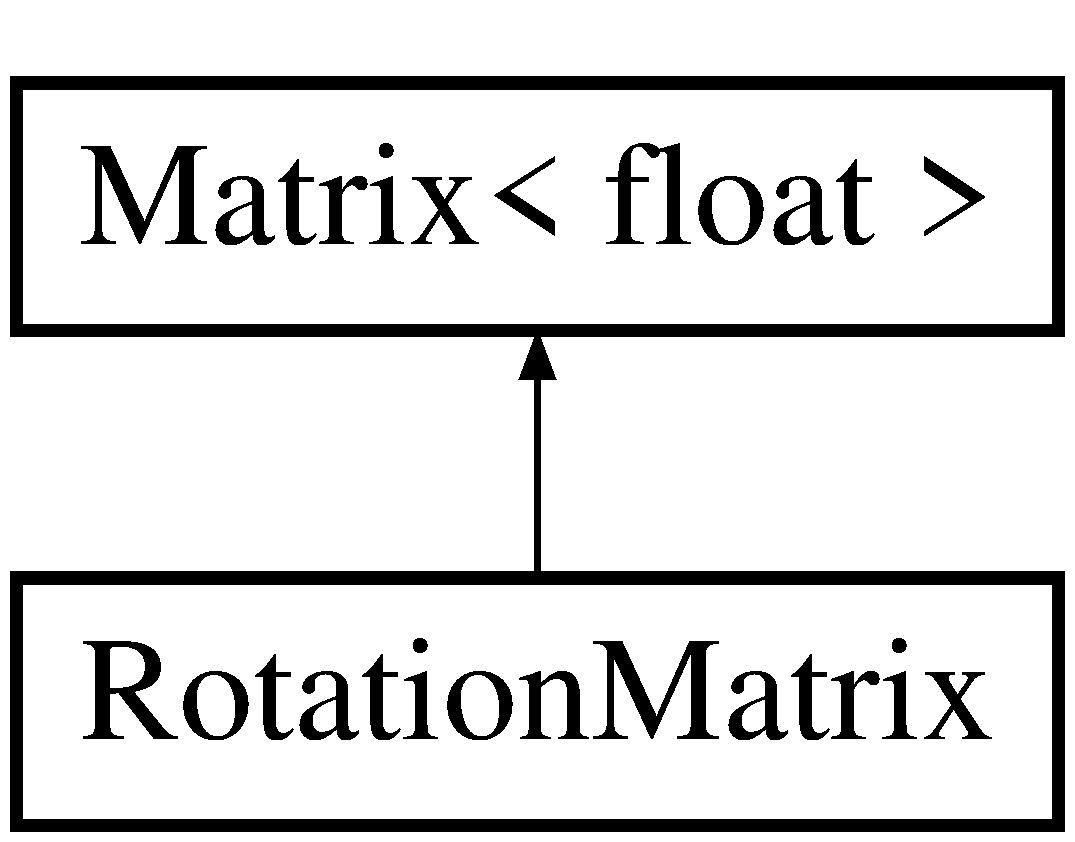
\includegraphics[height=2.000000cm]{class_rotation_matrix}
\end{center}
\end{figure}
\subsection*{Public Member Functions}
\begin{DoxyCompactItemize}
\item 
\hypertarget{class_rotation_matrix_a97bcf26df695672b768ec0009355b0fb}{\hyperlink{class_rotation_matrix_a97bcf26df695672b768ec0009355b0fb}{Rotation\+Matrix} (const float kf\+Radians)}\label{class_rotation_matrix_a97bcf26df695672b768ec0009355b0fb}

\begin{DoxyCompactList}\small\item\em Default constructor. \end{DoxyCompactList}\item 
void \hyperlink{class_rotation_matrix_a40d79c7eef78770b19024dc6776ee8c3}{set\+Angle\+Deg} (const float kf\+Degrees)
\begin{DoxyCompactList}\small\item\em Constructor which takes a radians value. \end{DoxyCompactList}\item 
void \hyperlink{class_rotation_matrix_a49c861f624a5a251a013684824cd51de}{set\+Angle\+Rad} (const float kf\+Radians)
\begin{DoxyCompactList}\small\item\em Takes an angle in radians and sets the angle. \end{DoxyCompactList}\item 
float \hyperlink{class_rotation_matrix_a012ca643690e92bf67357f703629010e}{get\+Angle\+Rad} () const 
\begin{DoxyCompactList}\small\item\em Returns the angle in radians. \end{DoxyCompactList}\item 
float \hyperlink{class_rotation_matrix_affe59fa1cb44c08e8341e46383f137c3}{get\+Angle\+Deg} () const 
\begin{DoxyCompactList}\small\item\em Returns the angle in degrees. \end{DoxyCompactList}\item 
\hypertarget{class_rotation_matrix_a5b1f1ef7de82392ae1f295c8356b3261}{\hyperlink{class_vector2_d}{Vector2\+D}$<$ float $>$ {\bfseries column1} () const }\label{class_rotation_matrix_a5b1f1ef7de82392ae1f295c8356b3261}

\item 
\hypertarget{class_rotation_matrix_af54d2979b5913610f33e1867cd8635dd}{\hyperlink{class_vector2_d}{Vector2\+D}$<$ float $>$ \hyperlink{class_rotation_matrix_af54d2979b5913610f33e1867cd8635dd}{column2} () const }\label{class_rotation_matrix_af54d2979b5913610f33e1867cd8635dd}

\begin{DoxyCompactList}\small\item\em Returns the first column as a vector. \end{DoxyCompactList}\item 
\hypertarget{class_rotation_matrix_ae1facb90c5f863cf19706211d7ea8ac9}{\hyperlink{class_vector2_d}{Vector2\+D}$<$ float $>$ \hyperlink{class_rotation_matrix_ae1facb90c5f863cf19706211d7ea8ac9}{row1} () const }\label{class_rotation_matrix_ae1facb90c5f863cf19706211d7ea8ac9}

\begin{DoxyCompactList}\small\item\em Returns the second column as a vector. \end{DoxyCompactList}\item 
\hypertarget{class_rotation_matrix_a81a16a06bfff94802cec97d6ff93c8e4}{\hyperlink{class_vector2_d}{Vector2\+D}$<$ float $>$ \hyperlink{class_rotation_matrix_a81a16a06bfff94802cec97d6ff93c8e4}{row2} () const }\label{class_rotation_matrix_a81a16a06bfff94802cec97d6ff93c8e4}

\begin{DoxyCompactList}\small\item\em Returns the first row as a vector. \end{DoxyCompactList}\item 
\hyperlink{class_vector2_d}{Vector2\+D}$<$ float $>$ \hyperlink{class_rotation_matrix_acf4a933168e87c20a622da9ddddc2022}{rotate\+Vector} (const \hyperlink{class_vector2_d}{Vector2\+D}$<$ float $>$ \&k\+Vec) const 
\begin{DoxyCompactList}\small\item\em Returns the second row as a vector. \end{DoxyCompactList}\item 
\hyperlink{class_vector2_d}{Vector2\+D}$<$ float $>$ \hyperlink{class_rotation_matrix_ad4a0fc37c2a155029bbb5f958ac0e1f7}{inverse\+Rotate\+Vector} (const \hyperlink{class_vector2_d}{Vector2\+D}$<$ float $>$ \&k\+Vec) const 
\begin{DoxyCompactList}\small\item\em Applies the inverse rotation to a vector. \end{DoxyCompactList}\end{DoxyCompactItemize}


\subsection{Detailed Description}
A 2\+D rotation matrix. 

\subsection{Member Function Documentation}
\hypertarget{class_rotation_matrix_affe59fa1cb44c08e8341e46383f137c3}{\index{Rotation\+Matrix@{Rotation\+Matrix}!get\+Angle\+Deg@{get\+Angle\+Deg}}
\index{get\+Angle\+Deg@{get\+Angle\+Deg}!Rotation\+Matrix@{Rotation\+Matrix}}
\subsubsection[{get\+Angle\+Deg}]{\setlength{\rightskip}{0pt plus 5cm}float Rotation\+Matrix\+::get\+Angle\+Deg (
\begin{DoxyParamCaption}
{}
\end{DoxyParamCaption}
) const}}\label{class_rotation_matrix_affe59fa1cb44c08e8341e46383f137c3}


Returns the angle in degrees. 

$<$ Returns the angle in degrees \hypertarget{class_rotation_matrix_a012ca643690e92bf67357f703629010e}{\index{Rotation\+Matrix@{Rotation\+Matrix}!get\+Angle\+Rad@{get\+Angle\+Rad}}
\index{get\+Angle\+Rad@{get\+Angle\+Rad}!Rotation\+Matrix@{Rotation\+Matrix}}
\subsubsection[{get\+Angle\+Rad}]{\setlength{\rightskip}{0pt plus 5cm}float Rotation\+Matrix\+::get\+Angle\+Rad (
\begin{DoxyParamCaption}
{}
\end{DoxyParamCaption}
) const}}\label{class_rotation_matrix_a012ca643690e92bf67357f703629010e}


Returns the angle in radians. 

$<$ Returns the angle in radians \hypertarget{class_rotation_matrix_ad4a0fc37c2a155029bbb5f958ac0e1f7}{\index{Rotation\+Matrix@{Rotation\+Matrix}!inverse\+Rotate\+Vector@{inverse\+Rotate\+Vector}}
\index{inverse\+Rotate\+Vector@{inverse\+Rotate\+Vector}!Rotation\+Matrix@{Rotation\+Matrix}}
\subsubsection[{inverse\+Rotate\+Vector}]{\setlength{\rightskip}{0pt plus 5cm}{\bf Vector2\+D}$<$ float $>$ Rotation\+Matrix\+::inverse\+Rotate\+Vector (
\begin{DoxyParamCaption}
\item[{const {\bf Vector2\+D}$<$ float $>$ \&}]{k\+Vec}
\end{DoxyParamCaption}
) const}}\label{class_rotation_matrix_ad4a0fc37c2a155029bbb5f958ac0e1f7}


Applies the inverse rotation to a vector. 

$<$ Applies the inverse rotation to a vector \hypertarget{class_rotation_matrix_acf4a933168e87c20a622da9ddddc2022}{\index{Rotation\+Matrix@{Rotation\+Matrix}!rotate\+Vector@{rotate\+Vector}}
\index{rotate\+Vector@{rotate\+Vector}!Rotation\+Matrix@{Rotation\+Matrix}}
\subsubsection[{rotate\+Vector}]{\setlength{\rightskip}{0pt plus 5cm}{\bf Vector2\+D}$<$ float $>$ Rotation\+Matrix\+::rotate\+Vector (
\begin{DoxyParamCaption}
\item[{const {\bf Vector2\+D}$<$ float $>$ \&}]{k\+Vec}
\end{DoxyParamCaption}
) const}}\label{class_rotation_matrix_acf4a933168e87c20a622da9ddddc2022}


Returns the second row as a vector. 

$<$ Applies the rotation to a vector

Applies the rotation to a vector \hypertarget{class_rotation_matrix_a40d79c7eef78770b19024dc6776ee8c3}{\index{Rotation\+Matrix@{Rotation\+Matrix}!set\+Angle\+Deg@{set\+Angle\+Deg}}
\index{set\+Angle\+Deg@{set\+Angle\+Deg}!Rotation\+Matrix@{Rotation\+Matrix}}
\subsubsection[{set\+Angle\+Deg}]{\setlength{\rightskip}{0pt plus 5cm}void Rotation\+Matrix\+::set\+Angle\+Deg (
\begin{DoxyParamCaption}
\item[{const float}]{kf\+Degrees}
\end{DoxyParamCaption}
)}}\label{class_rotation_matrix_a40d79c7eef78770b19024dc6776ee8c3}


Constructor which takes a radians value. 

Takes an angle in degrees and sets the angle 
\begin{DoxyParams}{Parameters}
{\em kf\+Degrees} & Takes an angle in degrees and sets the angle \\
\hline
\end{DoxyParams}
\hypertarget{class_rotation_matrix_a49c861f624a5a251a013684824cd51de}{\index{Rotation\+Matrix@{Rotation\+Matrix}!set\+Angle\+Rad@{set\+Angle\+Rad}}
\index{set\+Angle\+Rad@{set\+Angle\+Rad}!Rotation\+Matrix@{Rotation\+Matrix}}
\subsubsection[{set\+Angle\+Rad}]{\setlength{\rightskip}{0pt plus 5cm}void Rotation\+Matrix\+::set\+Angle\+Rad (
\begin{DoxyParamCaption}
\item[{const float}]{kf\+Radians}
\end{DoxyParamCaption}
)}}\label{class_rotation_matrix_a49c861f624a5a251a013684824cd51de}


Takes an angle in radians and sets the angle. 


\begin{DoxyParams}{Parameters}
{\em kf\+Radians} & Takes an angle in radians and sets the angle \\
\hline
\end{DoxyParams}


The documentation for this class was generated from the following files\+:\begin{DoxyCompactItemize}
\item 
include/\hyperlink{_rotation_matrix_8h}{Rotation\+Matrix.\+h}\item 
src/\hyperlink{_rotation_matrix_8cpp}{Rotation\+Matrix.\+cpp}\end{DoxyCompactItemize}

\hypertarget{struct_score_text_icons}{\section{Score\+Text\+Icons Struct Reference}
\label{struct_score_text_icons}\index{Score\+Text\+Icons@{Score\+Text\+Icons}}
}


a structure which contains a Text object and a timestamp  




{\ttfamily \#include $<$U\+I\+Manager.\+h$>$}

\subsection*{Public Attributes}
\begin{DoxyCompactItemize}
\item 
\hypertarget{struct_score_text_icons_af53518203f5368f0c646bc27f25cdb59}{sf\+::\+Text \hyperlink{struct_score_text_icons_af53518203f5368f0c646bc27f25cdb59}{m\+\_\+\+Text}}\label{struct_score_text_icons_af53518203f5368f0c646bc27f25cdb59}

\begin{DoxyCompactList}\small\item\em S\+F\+M\+L Text object. \end{DoxyCompactList}\item 
\hypertarget{struct_score_text_icons_aca94e73ec80d89215aace3f607997f4b}{sf\+::\+Time \hyperlink{struct_score_text_icons_aca94e73ec80d89215aace3f607997f4b}{m\+\_\+\+Time\+Stamp}}\label{struct_score_text_icons_aca94e73ec80d89215aace3f607997f4b}

\begin{DoxyCompactList}\small\item\em Timestamp. \end{DoxyCompactList}\end{DoxyCompactItemize}


\subsection{Detailed Description}
a structure which contains a Text object and a timestamp 

The documentation for this struct was generated from the following file\+:\begin{DoxyCompactItemize}
\item 
include/\hyperlink{_u_i_manager_8h}{U\+I\+Manager.\+h}\end{DoxyCompactItemize}

\hypertarget{class_spring}{\section{Spring Class Reference}
\label{class_spring}\index{Spring@{Spring}}
}
Inheritance diagram for Spring\+:\begin{figure}[H]
\begin{center}
\leavevmode
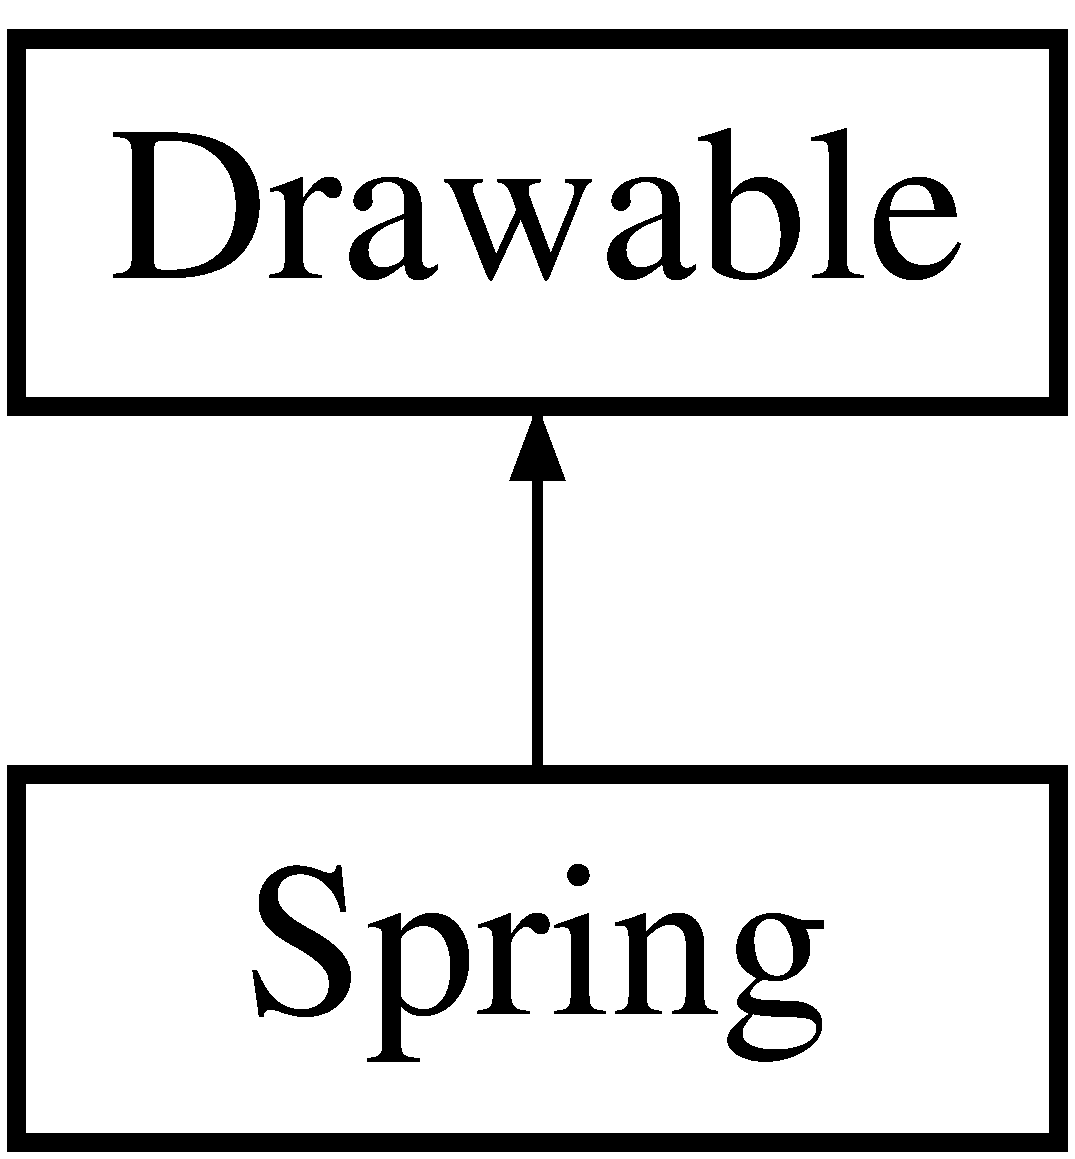
\includegraphics[height=2.000000cm]{class_spring}
\end{center}
\end{figure}
\subsection*{Public Member Functions}
\begin{DoxyCompactItemize}
\item 
\hypertarget{class_spring_aa452bf4d51b5a32834d4bca0805708a8}{virtual void {\bfseries draw} (sf\+::\+Render\+Target \&target, sf\+::\+Render\+States states) const }\label{class_spring_aa452bf4d51b5a32834d4bca0805708a8}

\item 
\hypertarget{class_spring_a8f0314e062615fd3989a2dc864096715}{void {\bfseries release} ()}\label{class_spring_a8f0314e062615fd3989a2dc864096715}

\item 
\hypertarget{class_spring_a5aa89d21be823e302129b06fb8192c2d}{void {\bfseries update} ()}\label{class_spring_a5aa89d21be823e302129b06fb8192c2d}

\item 
\hypertarget{class_spring_aa109f961a408a41608d77fda74ef8f38}{void {\bfseries down} ()}\label{class_spring_aa109f961a408a41608d77fda74ef8f38}

\end{DoxyCompactItemize}
\subsection*{Public Attributes}
\begin{DoxyCompactItemize}
\item 
\hypertarget{class_spring_aade9790be93c2eb83aae1146d24cd711}{std\+::shared\+\_\+ptr$<$ \hyperlink{class_body2_d}{Body2\+D} $>$ {\bfseries body}}\label{class_spring_aade9790be93c2eb83aae1146d24cd711}

\end{DoxyCompactItemize}


The documentation for this class was generated from the following files\+:\begin{DoxyCompactItemize}
\item 
include/\hyperlink{_spring_8h}{Spring.\+h}\item 
src/\hyperlink{_spring_8cpp}{Spring.\+cpp}\end{DoxyCompactItemize}

\hypertarget{class_sprite_manager}{\section{Sprite\+Manager Class Reference}
\label{class_sprite_manager}\index{Sprite\+Manager@{Sprite\+Manager}}
}


a manager for textures  




{\ttfamily \#include $<$Sprite\+Manager.\+h$>$}

\subsection*{Public Member Functions}
\begin{DoxyCompactItemize}
\item 
\hypertarget{class_sprite_manager_a757bd0abdc5551dd0420f7f7cfc81994}{\hyperlink{class_sprite_manager_a757bd0abdc5551dd0420f7f7cfc81994}{Sprite\+Manager} ()}\label{class_sprite_manager_a757bd0abdc5551dd0420f7f7cfc81994}

\begin{DoxyCompactList}\small\item\em Default Constructor. \end{DoxyCompactList}\item 
sf\+::\+Texture \hyperlink{class_sprite_manager_a13066fcf064d41630421e9d1a83fbe11}{get\+Texture} (const std\+::string \&s\+Name)
\begin{DoxyCompactList}\small\item\em Retrieve a texture with name. \end{DoxyCompactList}\end{DoxyCompactItemize}


\subsection{Detailed Description}
a manager for textures 

\subsection{Member Function Documentation}
\hypertarget{class_sprite_manager_a13066fcf064d41630421e9d1a83fbe11}{\index{Sprite\+Manager@{Sprite\+Manager}!get\+Texture@{get\+Texture}}
\index{get\+Texture@{get\+Texture}!Sprite\+Manager@{Sprite\+Manager}}
\subsubsection[{get\+Texture}]{\setlength{\rightskip}{0pt plus 5cm}sf\+::\+Texture Sprite\+Manager\+::get\+Texture (
\begin{DoxyParamCaption}
\item[{const std\+::string \&}]{s\+Name}
\end{DoxyParamCaption}
)}}\label{class_sprite_manager_a13066fcf064d41630421e9d1a83fbe11}


Retrieve a texture with name. 


\begin{DoxyParams}{Parameters}
{\em s\+Name} & Name of the texture \\
\hline
\end{DoxyParams}


The documentation for this class was generated from the following files\+:\begin{DoxyCompactItemize}
\item 
include/\hyperlink{_sprite_manager_8h}{Sprite\+Manager.\+h}\item 
src/\hyperlink{_sprite_manager_8cpp}{Sprite\+Manager.\+cpp}\end{DoxyCompactItemize}

\hypertarget{class_u_i_manager}{\section{U\+I\+Manager Class Reference}
\label{class_u_i_manager}\index{U\+I\+Manager@{U\+I\+Manager}}
}


Manages user interface and certain gameplay values.  




{\ttfamily \#include $<$U\+I\+Manager.\+h$>$}

Inheritance diagram for U\+I\+Manager\+:\begin{figure}[H]
\begin{center}
\leavevmode
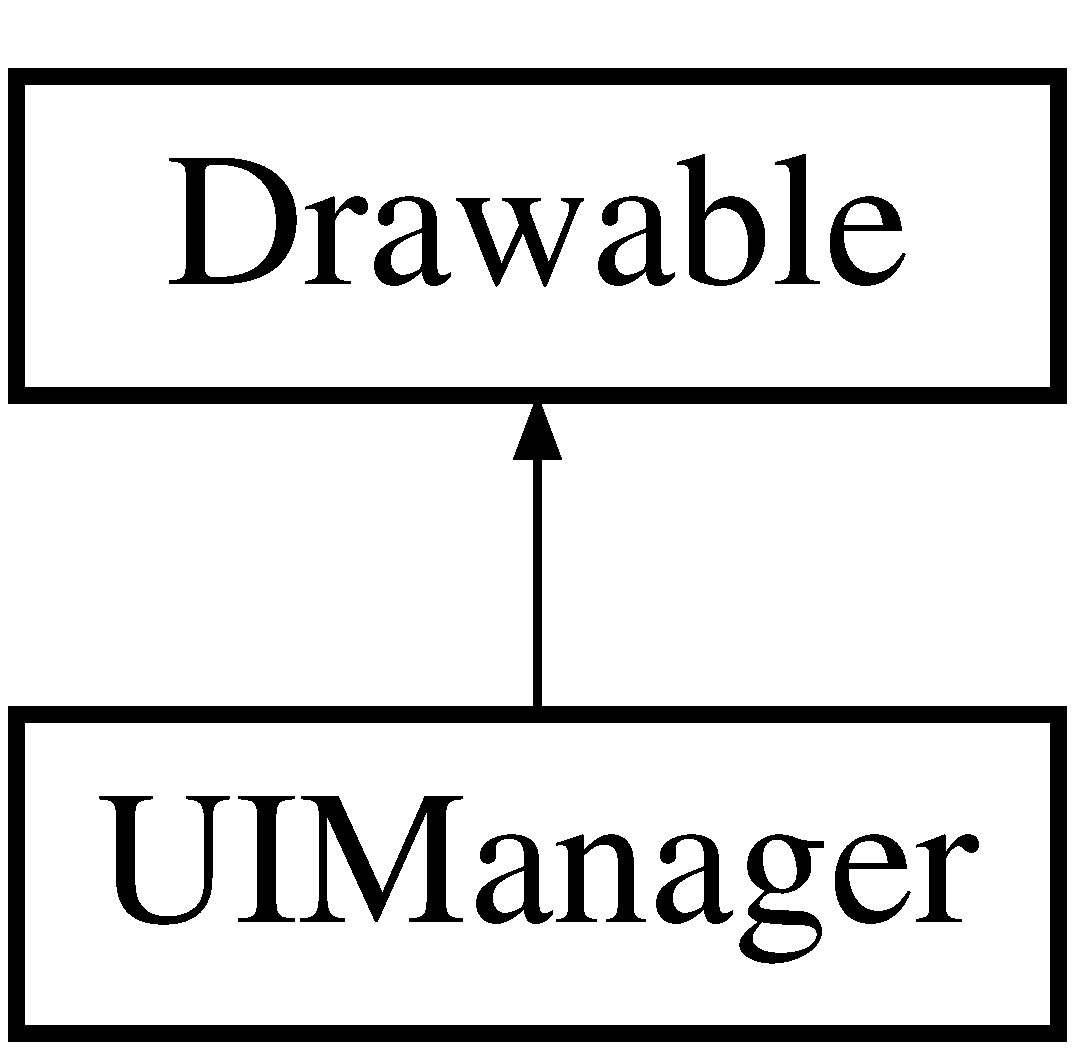
\includegraphics[height=2.000000cm]{class_u_i_manager}
\end{center}
\end{figure}
\subsection*{Public Member Functions}
\begin{DoxyCompactItemize}
\item 
\hypertarget{class_u_i_manager_a32b72c377f864f7cd197e6ffe738142f}{\hyperlink{class_u_i_manager_a32b72c377f864f7cd197e6ffe738142f}{U\+I\+Manager} ()}\label{class_u_i_manager_a32b72c377f864f7cd197e6ffe738142f}

\begin{DoxyCompactList}\small\item\em Default constructor. \end{DoxyCompactList}\item 
\hyperlink{class_u_i_manager_a89c46c8540da2a38b859eaa5dfb4243a}{U\+I\+Manager} (sf\+::\+Font new\+Font)
\begin{DoxyCompactList}\small\item\em Constructor which takes a font. \end{DoxyCompactList}\item 
\hypertarget{class_u_i_manager_aeac3e2a8fd4ba49821ce653f4d2fa6b6}{\hyperlink{class_u_i_manager_aeac3e2a8fd4ba49821ce653f4d2fa6b6}{$\sim$\+U\+I\+Manager} ()}\label{class_u_i_manager_aeac3e2a8fd4ba49821ce653f4d2fa6b6}

\begin{DoxyCompactList}\small\item\em Destructor. \end{DoxyCompactList}\item 
\hypertarget{class_u_i_manager_afcb9f18d87b7e95ad5632bffeb48f56f}{void \hyperlink{class_u_i_manager_afcb9f18d87b7e95ad5632bffeb48f56f}{remove\+Life} ()}\label{class_u_i_manager_afcb9f18d87b7e95ad5632bffeb48f56f}

\begin{DoxyCompactList}\small\item\em Remove a player life. \end{DoxyCompactList}\item 
\hypertarget{class_u_i_manager_aff0a63e6d0d7ae9f26cdd415c3151f3f}{void \hyperlink{class_u_i_manager_aff0a63e6d0d7ae9f26cdd415c3151f3f}{new\+Game} ()}\label{class_u_i_manager_aff0a63e6d0d7ae9f26cdd415c3151f3f}

\begin{DoxyCompactList}\small\item\em Setup for a new game. \end{DoxyCompactList}\item 
void \hyperlink{class_u_i_manager_a910958d4ba0efde343fdaa041f550acd}{save\+File} () const 
\begin{DoxyCompactList}\small\item\em Saves the highscore to a text file. \end{DoxyCompactList}\item 
void \hyperlink{class_u_i_manager_a783b2d2f87f16ea45875114f92856950}{add\+Points} (const unsigned int kui\+Add\+Points)
\item 
void \hyperlink{class_u_i_manager_a721a50436f0c9584b19ee646b407289e}{add\+Points\+Animated} (const unsigned int kui\+Add\+Points, const \hyperlink{class_vector2_d}{Vector2\+D}$<$ float $>$ \&k\+Position)
\begin{DoxyCompactList}\small\item\em Takes an unsigned integer and adds it to the player score. \end{DoxyCompactList}\item 
\hypertarget{class_u_i_manager_a12ed6f32d28d232782c5bdbbb09b3c9f}{void \hyperlink{class_u_i_manager_a12ed6f32d28d232782c5bdbbb09b3c9f}{update} ()}\label{class_u_i_manager_a12ed6f32d28d232782c5bdbbb09b3c9f}

\begin{DoxyCompactList}\small\item\em Updates the logic. \end{DoxyCompactList}\item 
virtual void \hyperlink{class_u_i_manager_a5b561519f60c7b5e59c010794715b564}{draw} (sf\+::\+Render\+Target \&target, sf\+::\+Render\+States states) const 
\begin{DoxyCompactList}\small\item\em Draw the user interface. \end{DoxyCompactList}\end{DoxyCompactItemize}
\subsection*{Public Attributes}
\begin{DoxyCompactItemize}
\item 
\hypertarget{class_u_i_manager_a126f5ffe70cdd465e492f7af57c00b1e}{int \hyperlink{class_u_i_manager_a126f5ffe70cdd465e492f7af57c00b1e}{ui\+Lives}}\label{class_u_i_manager_a126f5ffe70cdd465e492f7af57c00b1e}

\begin{DoxyCompactList}\small\item\em Player lives. \end{DoxyCompactList}\end{DoxyCompactItemize}


\subsection{Detailed Description}
Manages user interface and certain gameplay values. 

\subsection{Constructor \& Destructor Documentation}
\hypertarget{class_u_i_manager_a89c46c8540da2a38b859eaa5dfb4243a}{\index{U\+I\+Manager@{U\+I\+Manager}!U\+I\+Manager@{U\+I\+Manager}}
\index{U\+I\+Manager@{U\+I\+Manager}!U\+I\+Manager@{U\+I\+Manager}}
\subsubsection[{U\+I\+Manager}]{\setlength{\rightskip}{0pt plus 5cm}U\+I\+Manager\+::\+U\+I\+Manager (
\begin{DoxyParamCaption}
\item[{sf\+::\+Font}]{new\+Font}
\end{DoxyParamCaption}
)}}\label{class_u_i_manager_a89c46c8540da2a38b859eaa5dfb4243a}


Constructor which takes a font. 


\begin{DoxyParams}{Parameters}
{\em new\+Font} & Font value \\
\hline
\end{DoxyParams}


\subsection{Member Function Documentation}
\hypertarget{class_u_i_manager_a783b2d2f87f16ea45875114f92856950}{\index{U\+I\+Manager@{U\+I\+Manager}!add\+Points@{add\+Points}}
\index{add\+Points@{add\+Points}!U\+I\+Manager@{U\+I\+Manager}}
\subsubsection[{add\+Points}]{\setlength{\rightskip}{0pt plus 5cm}void U\+I\+Manager\+::add\+Points (
\begin{DoxyParamCaption}
\item[{const unsigned int}]{kui\+Add\+Points}
\end{DoxyParamCaption}
)\hspace{0.3cm}{\ttfamily [inline]}}}\label{class_u_i_manager_a783b2d2f87f16ea45875114f92856950}

\begin{DoxyParams}{Parameters}
{\em kui\+Add\+Points} & Points value \\
\hline
\end{DoxyParams}
\hypertarget{class_u_i_manager_a721a50436f0c9584b19ee646b407289e}{\index{U\+I\+Manager@{U\+I\+Manager}!add\+Points\+Animated@{add\+Points\+Animated}}
\index{add\+Points\+Animated@{add\+Points\+Animated}!U\+I\+Manager@{U\+I\+Manager}}
\subsubsection[{add\+Points\+Animated}]{\setlength{\rightskip}{0pt plus 5cm}void U\+I\+Manager\+::add\+Points\+Animated (
\begin{DoxyParamCaption}
\item[{const unsigned int}]{kui\+Add\+Points, }
\item[{const {\bf Vector2\+D}$<$ float $>$ \&}]{k\+Position}
\end{DoxyParamCaption}
)}}\label{class_u_i_manager_a721a50436f0c9584b19ee646b407289e}


Takes an unsigned integer and adds it to the player score. 

Takes an unsigned integer and adds it to the player score and takes a \hyperlink{class_vector2_d}{Vector2\+D} to position the animated icon 
\begin{DoxyParams}{Parameters}
{\em kui\+Add\+Points} & Points value \\
\hline
{\em k\+Position} & Vector position \\
\hline
\end{DoxyParams}
\hypertarget{class_u_i_manager_a5b561519f60c7b5e59c010794715b564}{\index{U\+I\+Manager@{U\+I\+Manager}!draw@{draw}}
\index{draw@{draw}!U\+I\+Manager@{U\+I\+Manager}}
\subsubsection[{draw}]{\setlength{\rightskip}{0pt plus 5cm}void U\+I\+Manager\+::draw (
\begin{DoxyParamCaption}
\item[{sf\+::\+Render\+Target \&}]{target, }
\item[{sf\+::\+Render\+States}]{states}
\end{DoxyParamCaption}
) const\hspace{0.3cm}{\ttfamily [virtual]}}}\label{class_u_i_manager_a5b561519f60c7b5e59c010794715b564}


Draw the user interface. 

$<$ Draw the user interface \hypertarget{class_u_i_manager_a910958d4ba0efde343fdaa041f550acd}{\index{U\+I\+Manager@{U\+I\+Manager}!save\+File@{save\+File}}
\index{save\+File@{save\+File}!U\+I\+Manager@{U\+I\+Manager}}
\subsubsection[{save\+File}]{\setlength{\rightskip}{0pt plus 5cm}void U\+I\+Manager\+::save\+File (
\begin{DoxyParamCaption}
{}
\end{DoxyParamCaption}
) const}}\label{class_u_i_manager_a910958d4ba0efde343fdaa041f550acd}


Saves the highscore to a text file. 

$<$ Saves the highscore to a text file 

The documentation for this class was generated from the following files\+:\begin{DoxyCompactItemize}
\item 
include/\hyperlink{_u_i_manager_8h}{U\+I\+Manager.\+h}\item 
src/\hyperlink{_u_i_manager_8cpp}{U\+I\+Manager.\+cpp}\end{DoxyCompactItemize}

\hypertarget{class_vector2_d}{\section{Vector2\+D$<$ N $>$ Class Template Reference}
\label{class_vector2_d}\index{Vector2\+D$<$ N $>$@{Vector2\+D$<$ N $>$}}
}


A 2\+D vector template.  




{\ttfamily \#include $<$Vector2\+D.\+h$>$}

\subsection*{Public Member Functions}
\begin{DoxyCompactItemize}
\item 
\hyperlink{class_vector2_d_a289953197d4b246d198df2bd9997185e}{Vector2\+D} (const N k\+All\+Values)
\begin{DoxyCompactList}\small\item\em Default constuctor (sets all values to 0) \end{DoxyCompactList}\item 
\hyperlink{class_vector2_d_aac592df4ad03808d237ac31917ec902a}{Vector2\+D} (const N k\+X, const N k\+Y)
\begin{DoxyCompactList}\small\item\em Constructor which take a number to assign all values. \end{DoxyCompactList}\item 
void \hyperlink{class_vector2_d_a384d0e05609df11eef36118abc95789c}{set} (const N k\+X, const N k\+Y)
\begin{DoxyCompactList}\small\item\em Constructor which takes X and Y values. \end{DoxyCompactList}\item 
void \hyperlink{class_vector2_d_a63de9a5ad26934fc4d6df9111db3bd3f}{set\+X} (const N k\+X)
\begin{DoxyCompactList}\small\item\em Sets the X and Y values. \end{DoxyCompactList}\item 
void \hyperlink{class_vector2_d_acd9f8f5aa8f9b5ce8c4212638eee8c24}{set\+Y} (const N k\+Y)
\begin{DoxyCompactList}\small\item\em Sets the X value. \end{DoxyCompactList}\item 
float \hyperlink{class_vector2_d_a470b4b79c5bad154922113a7fd4272ee}{angle} (const \hyperlink{class_vector2_d}{Vector2\+D}$<$ N $>$ \&other) const 
\begin{DoxyCompactList}\small\item\em Sets the Y value. \end{DoxyCompactList}\item 
float \hyperlink{class_vector2_d_a0454fdd76683b17dc456c9d1b5ac9166}{dot\+Product} (const \hyperlink{class_vector2_d}{Vector2\+D}$<$ N $>$ \&other) const 
\item 
float \hyperlink{class_vector2_d_a9f41b23b1b0cf0b6d68772f8642ad7f1}{cross\+Product} (const \hyperlink{class_vector2_d}{Vector2\+D}$<$ N $>$ \&other) const 
\begin{DoxyCompactList}\small\item\em Returns the dot product of the current vector and another vector. \end{DoxyCompactList}\item 
\hyperlink{class_vector2_d}{Vector2\+D}$<$ N $>$ \hyperlink{class_vector2_d_ae270e23529e253fe49e1a8d98b059d73}{cross\+Product} (const float kf\+Scalar) const 
\begin{DoxyCompactList}\small\item\em Returns the cross product of the current vector and another vector. \end{DoxyCompactList}\item 
\hyperlink{class_vector2_d}{Vector2\+D}$<$ float $>$ \hyperlink{class_vector2_d_a17f850d113f71036587f573fc7acd7f7}{cross\+Product} (const float kf\+Scalar, const \hyperlink{class_vector2_d}{Vector2\+D}$<$ float $>$ \&k\+Vec) const 
\begin{DoxyCompactList}\small\item\em Returns the cross product of the vector. \end{DoxyCompactList}\item 
\hypertarget{class_vector2_d_a00aac8564c3e98d800fa3687ca159f91}{\hyperlink{class_vector2_d}{Vector2\+D}$<$ N $>$ {\bfseries unit\+Vector} () const }\label{class_vector2_d_a00aac8564c3e98d800fa3687ca159f91}

\item 
\hypertarget{class_vector2_d_adc7c5d679051dc6c8b6a1c6ee3c5abbf}{N \hyperlink{class_vector2_d_adc7c5d679051dc6c8b6a1c6ee3c5abbf}{x} () const }\label{class_vector2_d_adc7c5d679051dc6c8b6a1c6ee3c5abbf}

\begin{DoxyCompactList}\small\item\em Returns the unit vector. \end{DoxyCompactList}\item 
\hypertarget{class_vector2_d_a3b3d6a9a07bba8871954400d92f233d7}{N \hyperlink{class_vector2_d_a3b3d6a9a07bba8871954400d92f233d7}{y} () const }\label{class_vector2_d_a3b3d6a9a07bba8871954400d92f233d7}

\begin{DoxyCompactList}\small\item\em Returns the X value of the vector. \end{DoxyCompactList}\item 
\hypertarget{class_vector2_d_a9f7e7889fad81bd9ee74e1b13971f9c8}{float \hyperlink{class_vector2_d_a9f7e7889fad81bd9ee74e1b13971f9c8}{magnitude} () const }\label{class_vector2_d_a9f7e7889fad81bd9ee74e1b13971f9c8}

\begin{DoxyCompactList}\small\item\em Returns the Y value of the vector. \end{DoxyCompactList}\item 
\hypertarget{class_vector2_d_a8987f5af709e06776682cb76774ec54e}{float \hyperlink{class_vector2_d_a8987f5af709e06776682cb76774ec54e}{magnitude\+Squared} () const }\label{class_vector2_d_a8987f5af709e06776682cb76774ec54e}

\begin{DoxyCompactList}\small\item\em Returns the magnitude of the vector. \end{DoxyCompactList}\item 
\hyperlink{class_vector2_d}{Vector2\+D}$<$ N $>$ \hyperlink{class_vector2_d_abe4ad594ca6c0ef36514452006727a05}{operator-\/} (const \hyperlink{class_vector2_d}{Vector2\+D}$<$ N $>$ \&k\+Other) const 
\begin{DoxyCompactList}\small\item\em Returns the square of the length of the vector2\+D. \end{DoxyCompactList}\item 
\hyperlink{class_vector2_d}{Vector2\+D}$<$ N $>$ \hyperlink{class_vector2_d_ab85731551989b97ca8a3d72804a1b751}{operator-\/} (const float kf\+Scalar) const 
\begin{DoxyCompactList}\small\item\em Returns the value of the current vector minus another vector. \end{DoxyCompactList}\item 
\hypertarget{class_vector2_d_a71521323d87489bccf35d711cf1068a4}{\hyperlink{class_vector2_d}{Vector2\+D}$<$ N $>$ \hyperlink{class_vector2_d_a71521323d87489bccf35d711cf1068a4}{operator-\/} () const }\label{class_vector2_d_a71521323d87489bccf35d711cf1068a4}

\begin{DoxyCompactList}\small\item\em Returns the value of the current vector minus a float. \end{DoxyCompactList}\item 
\hyperlink{class_vector2_d}{Vector2\+D}$<$ N $>$ \& \hyperlink{class_vector2_d_a5db96bd2de56c4f1ebd426cfb4593e52}{operator-\/=} (const \hyperlink{class_vector2_d}{Vector2\+D}$<$ N $>$ \&k\+Other)
\begin{DoxyCompactList}\small\item\em Returns the negative of the vector. \end{DoxyCompactList}\item 
\hyperlink{class_vector2_d}{Vector2\+D}$<$ N $>$ \hyperlink{class_vector2_d_ac8f9fe8f4943e434537d67674265b388}{operator+} (const \hyperlink{class_vector2_d}{Vector2\+D}$<$ N $>$ \&k\+Other) const 
\begin{DoxyCompactList}\small\item\em Assigns the vector to its current value minus another vector. \end{DoxyCompactList}\item 
\hyperlink{class_vector2_d}{Vector2\+D}$<$ N $>$ \hyperlink{class_vector2_d_a450bb0c2588ff34f60edeb6d8d7d184f}{operator+} (const float kf\+Scalar) const 
\begin{DoxyCompactList}\small\item\em Returns the value of the current vector plus another vector. \end{DoxyCompactList}\item 
\hyperlink{class_vector2_d}{Vector2\+D}$<$ N $>$ \& \hyperlink{class_vector2_d_ad33289edb9a8c7e62aba24aaf3a28fef}{operator+=} (const \hyperlink{class_vector2_d}{Vector2\+D}$<$ N $>$ \&k\+Other)
\begin{DoxyCompactList}\small\item\em Returns the value of the current vector plus a float. \end{DoxyCompactList}\item 
\hyperlink{class_vector2_d}{Vector2\+D}$<$ N $>$ \hyperlink{class_vector2_d_a4577730fdb261a2e56065ee23ee551e3}{operator$\ast$} (const \hyperlink{class_vector2_d}{Vector2\+D}$<$ N $>$ \&k\+Other) const 
\begin{DoxyCompactList}\small\item\em Assigns the vector to its current value plus another vector. \end{DoxyCompactList}\item 
\hyperlink{class_vector2_d}{Vector2\+D}$<$ N $>$ \& \hyperlink{class_vector2_d_a6ff7b67451e0c66d58e1844d02598e49}{operator$\ast$=} (const \hyperlink{class_vector2_d}{Vector2\+D}$<$ N $>$ \&k\+Other)
\begin{DoxyCompactList}\small\item\em Returns the value of the current vector multiplied by another vector. \end{DoxyCompactList}\item 
\hyperlink{class_vector2_d}{Vector2\+D}$<$ N $>$ \hyperlink{class_vector2_d_ab166d50dcd7fe7650982ec8ae7a87d1f}{operator/} (const \hyperlink{class_vector2_d}{Vector2\+D}$<$ N $>$ \&k\+Other) const 
\begin{DoxyCompactList}\small\item\em Assigns the vector to its current value multiplied by another vector. \end{DoxyCompactList}\item 
\hyperlink{class_vector2_d}{Vector2\+D}$<$ N $>$ \hyperlink{class_vector2_d_a23981e8ae406ff535d8b08863d332965}{operator$\ast$} (const float kf\+Scalar) const 
\begin{DoxyCompactList}\small\item\em Returns the value of the current vector divided by another vector. \end{DoxyCompactList}\item 
\hyperlink{class_vector2_d}{Vector2\+D}$<$ N $>$ \hyperlink{class_vector2_d_ae4dbe6b165e3def7664dfbc522bf25ac}{operator/} (const float kf\+Scalar) const 
\begin{DoxyCompactList}\small\item\em Returns the value of the current vector multiplied by a float. \end{DoxyCompactList}\item 
\hyperlink{class_vector2_d}{Vector2\+D}$<$ N $>$ \& \hyperlink{class_vector2_d_a2057096e75e930ca74ddcf25aa114da7}{operator/=} (const \hyperlink{class_vector2_d}{Vector2\+D}$<$ N $>$ \&k\+Other)
\begin{DoxyCompactList}\small\item\em Returns the value of the current vector divided by a float. \end{DoxyCompactList}\item 
\hyperlink{class_vector2_d}{Vector2\+D}$<$ N $>$ \& \hyperlink{class_vector2_d_a559a75132a11f73c1d8f9cc548f14fd2}{operator/=} (const float kf\+Scalar)
\begin{DoxyCompactList}\small\item\em Assigns the vector to its current value divided by another vector. \end{DoxyCompactList}\item 
\hyperlink{class_vector2_d}{Vector2\+D}$<$ N $>$ \& \hyperlink{class_vector2_d_a8b88b4dd0feaec5794f2904b86ac2c09}{operator=} (const \hyperlink{class_vector2_d}{Vector2\+D}$<$ N $>$ \&k\+Other)
\begin{DoxyCompactList}\small\item\em Assigns the vector to its current value divided by a float scalar. \end{DoxyCompactList}\item 
bool \hyperlink{class_vector2_d_a89655cac99d0f6288eaf649396cbeef1}{operator==} (const \hyperlink{class_vector2_d}{Vector2\+D}$<$ N $>$ \&k\+Other) const 
\begin{DoxyCompactList}\small\item\em Assigns the value of a vector to another vector. \end{DoxyCompactList}\item 
bool \hyperlink{class_vector2_d_a829da096b8e39d2ef47f0f03b33609bd}{operator!=} (const \hyperlink{class_vector2_d}{Vector2\+D}$<$ N $>$ \&k\+Other) const 
\begin{DoxyCompactList}\small\item\em Returns true if the current vector has the same value as another vector. \end{DoxyCompactList}\end{DoxyCompactItemize}


\subsection{Detailed Description}
\subsubsection*{template$<$class N$>$class Vector2\+D$<$ N $>$}

A 2\+D vector template. 

\subsection{Constructor \& Destructor Documentation}
\hypertarget{class_vector2_d_a289953197d4b246d198df2bd9997185e}{\index{Vector2\+D@{Vector2\+D}!Vector2\+D@{Vector2\+D}}
\index{Vector2\+D@{Vector2\+D}!Vector2\+D@{Vector2\+D}}
\subsubsection[{Vector2\+D}]{\setlength{\rightskip}{0pt plus 5cm}template$<$class N$>$ {\bf Vector2\+D}$<$ N $>$\+::{\bf Vector2\+D} (
\begin{DoxyParamCaption}
\item[{const N}]{k\+All\+Values}
\end{DoxyParamCaption}
)\hspace{0.3cm}{\ttfamily [inline]}}}\label{class_vector2_d_a289953197d4b246d198df2bd9997185e}


Default constuctor (sets all values to 0) 


\begin{DoxyParams}{Parameters}
{\em k\+All\+Values} & Float to apply to both X and Y values \\
\hline
\end{DoxyParams}
\hypertarget{class_vector2_d_aac592df4ad03808d237ac31917ec902a}{\index{Vector2\+D@{Vector2\+D}!Vector2\+D@{Vector2\+D}}
\index{Vector2\+D@{Vector2\+D}!Vector2\+D@{Vector2\+D}}
\subsubsection[{Vector2\+D}]{\setlength{\rightskip}{0pt plus 5cm}template$<$class N$>$ {\bf Vector2\+D}$<$ N $>$\+::{\bf Vector2\+D} (
\begin{DoxyParamCaption}
\item[{const N}]{k\+X, }
\item[{const N}]{k\+Y}
\end{DoxyParamCaption}
)\hspace{0.3cm}{\ttfamily [inline]}}}\label{class_vector2_d_aac592df4ad03808d237ac31917ec902a}


Constructor which take a number to assign all values. 


\begin{DoxyParams}{Parameters}
{\em k\+X} & X value \\
\hline
{\em k\+Y} & Y value \\
\hline
\end{DoxyParams}


\subsection{Member Function Documentation}
\hypertarget{class_vector2_d_a470b4b79c5bad154922113a7fd4272ee}{\index{Vector2\+D@{Vector2\+D}!angle@{angle}}
\index{angle@{angle}!Vector2\+D@{Vector2\+D}}
\subsubsection[{angle}]{\setlength{\rightskip}{0pt plus 5cm}template$<$class N$>$ float {\bf Vector2\+D}$<$ N $>$\+::angle (
\begin{DoxyParamCaption}
\item[{const {\bf Vector2\+D}$<$ N $>$ \&}]{other}
\end{DoxyParamCaption}
) const}}\label{class_vector2_d_a470b4b79c5bad154922113a7fd4272ee}


Sets the Y value. 

$<$ Returns the angle between the current vector2\+D and another vector2\+D

Returns the angle between the current vector2\+D and another vector2\+D 
\begin{DoxyParams}{Parameters}
{\em other} & Other vector \\
\hline
\end{DoxyParams}
\hypertarget{class_vector2_d_a9f41b23b1b0cf0b6d68772f8642ad7f1}{\index{Vector2\+D@{Vector2\+D}!cross\+Product@{cross\+Product}}
\index{cross\+Product@{cross\+Product}!Vector2\+D@{Vector2\+D}}
\subsubsection[{cross\+Product}]{\setlength{\rightskip}{0pt plus 5cm}template$<$class N$>$ float {\bf Vector2\+D}$<$ N $>$\+::cross\+Product (
\begin{DoxyParamCaption}
\item[{const {\bf Vector2\+D}$<$ N $>$ \&}]{other}
\end{DoxyParamCaption}
) const\hspace{0.3cm}{\ttfamily [inline]}}}\label{class_vector2_d_a9f41b23b1b0cf0b6d68772f8642ad7f1}


Returns the dot product of the current vector and another vector. 


\begin{DoxyParams}{Parameters}
{\em other} & Other vector \\
\hline
\end{DoxyParams}
\hypertarget{class_vector2_d_ae270e23529e253fe49e1a8d98b059d73}{\index{Vector2\+D@{Vector2\+D}!cross\+Product@{cross\+Product}}
\index{cross\+Product@{cross\+Product}!Vector2\+D@{Vector2\+D}}
\subsubsection[{cross\+Product}]{\setlength{\rightskip}{0pt plus 5cm}template$<$class N$>$ {\bf Vector2\+D}$<$N$>$ {\bf Vector2\+D}$<$ N $>$\+::cross\+Product (
\begin{DoxyParamCaption}
\item[{const float}]{kf\+Scalar}
\end{DoxyParamCaption}
) const\hspace{0.3cm}{\ttfamily [inline]}}}\label{class_vector2_d_ae270e23529e253fe49e1a8d98b059d73}


Returns the cross product of the current vector and another vector. 


\begin{DoxyParams}{Parameters}
{\em kf\+Scalar} & Scalar value \\
\hline
\end{DoxyParams}
\hypertarget{class_vector2_d_a17f850d113f71036587f573fc7acd7f7}{\index{Vector2\+D@{Vector2\+D}!cross\+Product@{cross\+Product}}
\index{cross\+Product@{cross\+Product}!Vector2\+D@{Vector2\+D}}
\subsubsection[{cross\+Product}]{\setlength{\rightskip}{0pt plus 5cm}template$<$class N$>$ {\bf Vector2\+D}$<$float$>$ {\bf Vector2\+D}$<$ N $>$\+::cross\+Product (
\begin{DoxyParamCaption}
\item[{const float}]{kf\+Scalar, }
\item[{const {\bf Vector2\+D}$<$ float $>$ \&}]{k\+Vec}
\end{DoxyParamCaption}
) const\hspace{0.3cm}{\ttfamily [inline]}}}\label{class_vector2_d_a17f850d113f71036587f573fc7acd7f7}


Returns the cross product of the vector. 

Returns the cross product of a scalar and a vector 
\begin{DoxyParams}{Parameters}
{\em kf\+Scalar} & Scalar value \\
\hline
{\em k\+Vec} & vector \\
\hline
\end{DoxyParams}
\hypertarget{class_vector2_d_a0454fdd76683b17dc456c9d1b5ac9166}{\index{Vector2\+D@{Vector2\+D}!dot\+Product@{dot\+Product}}
\index{dot\+Product@{dot\+Product}!Vector2\+D@{Vector2\+D}}
\subsubsection[{dot\+Product}]{\setlength{\rightskip}{0pt plus 5cm}template$<$class N$>$ float {\bf Vector2\+D}$<$ N $>$\+::dot\+Product (
\begin{DoxyParamCaption}
\item[{const {\bf Vector2\+D}$<$ N $>$ \&}]{other}
\end{DoxyParamCaption}
) const\hspace{0.3cm}{\ttfamily [inline]}}}\label{class_vector2_d_a0454fdd76683b17dc456c9d1b5ac9166}

\begin{DoxyParams}{Parameters}
{\em other} & Other vector \\
\hline
\end{DoxyParams}
\hypertarget{class_vector2_d_a829da096b8e39d2ef47f0f03b33609bd}{\index{Vector2\+D@{Vector2\+D}!operator"!=@{operator"!=}}
\index{operator"!=@{operator"!=}!Vector2\+D@{Vector2\+D}}
\subsubsection[{operator"!=}]{\setlength{\rightskip}{0pt plus 5cm}template$<$class N$>$ bool {\bf Vector2\+D}$<$ N $>$\+::operator!= (
\begin{DoxyParamCaption}
\item[{const {\bf Vector2\+D}$<$ N $>$ \&}]{k\+Other}
\end{DoxyParamCaption}
) const\hspace{0.3cm}{\ttfamily [inline]}}}\label{class_vector2_d_a829da096b8e39d2ef47f0f03b33609bd}


Returns true if the current vector has the same value as another vector. 


\begin{DoxyParams}{Parameters}
{\em k\+Other} & Other vector \\
\hline
\end{DoxyParams}
\hypertarget{class_vector2_d_a4577730fdb261a2e56065ee23ee551e3}{\index{Vector2\+D@{Vector2\+D}!operator$\ast$@{operator$\ast$}}
\index{operator$\ast$@{operator$\ast$}!Vector2\+D@{Vector2\+D}}
\subsubsection[{operator$\ast$}]{\setlength{\rightskip}{0pt plus 5cm}template$<$class N$>$ {\bf Vector2\+D}$<$N$>$ {\bf Vector2\+D}$<$ N $>$\+::operator$\ast$ (
\begin{DoxyParamCaption}
\item[{const {\bf Vector2\+D}$<$ N $>$ \&}]{k\+Other}
\end{DoxyParamCaption}
) const\hspace{0.3cm}{\ttfamily [inline]}}}\label{class_vector2_d_a4577730fdb261a2e56065ee23ee551e3}


Assigns the vector to its current value plus another vector. 


\begin{DoxyParams}{Parameters}
{\em k\+Other} & Other vector \\
\hline
\end{DoxyParams}
\hypertarget{class_vector2_d_a23981e8ae406ff535d8b08863d332965}{\index{Vector2\+D@{Vector2\+D}!operator$\ast$@{operator$\ast$}}
\index{operator$\ast$@{operator$\ast$}!Vector2\+D@{Vector2\+D}}
\subsubsection[{operator$\ast$}]{\setlength{\rightskip}{0pt plus 5cm}template$<$class N$>$ {\bf Vector2\+D}$<$N$>$ {\bf Vector2\+D}$<$ N $>$\+::operator$\ast$ (
\begin{DoxyParamCaption}
\item[{const float}]{kf\+Scalar}
\end{DoxyParamCaption}
) const\hspace{0.3cm}{\ttfamily [inline]}}}\label{class_vector2_d_a23981e8ae406ff535d8b08863d332965}


Returns the value of the current vector divided by another vector. 


\begin{DoxyParams}{Parameters}
{\em kf\+Scalar} & Scalar value \\
\hline
\end{DoxyParams}
\hypertarget{class_vector2_d_a6ff7b67451e0c66d58e1844d02598e49}{\index{Vector2\+D@{Vector2\+D}!operator$\ast$=@{operator$\ast$=}}
\index{operator$\ast$=@{operator$\ast$=}!Vector2\+D@{Vector2\+D}}
\subsubsection[{operator$\ast$=}]{\setlength{\rightskip}{0pt plus 5cm}template$<$class N$>$ {\bf Vector2\+D}$<$N$>$\& {\bf Vector2\+D}$<$ N $>$\+::operator$\ast$= (
\begin{DoxyParamCaption}
\item[{const {\bf Vector2\+D}$<$ N $>$ \&}]{k\+Other}
\end{DoxyParamCaption}
)\hspace{0.3cm}{\ttfamily [inline]}}}\label{class_vector2_d_a6ff7b67451e0c66d58e1844d02598e49}


Returns the value of the current vector multiplied by another vector. 


\begin{DoxyParams}{Parameters}
{\em k\+Other} & Other vector \\
\hline
\end{DoxyParams}
\hypertarget{class_vector2_d_ac8f9fe8f4943e434537d67674265b388}{\index{Vector2\+D@{Vector2\+D}!operator+@{operator+}}
\index{operator+@{operator+}!Vector2\+D@{Vector2\+D}}
\subsubsection[{operator+}]{\setlength{\rightskip}{0pt plus 5cm}template$<$class N$>$ {\bf Vector2\+D}$<$N$>$ {\bf Vector2\+D}$<$ N $>$\+::operator+ (
\begin{DoxyParamCaption}
\item[{const {\bf Vector2\+D}$<$ N $>$ \&}]{k\+Other}
\end{DoxyParamCaption}
) const\hspace{0.3cm}{\ttfamily [inline]}}}\label{class_vector2_d_ac8f9fe8f4943e434537d67674265b388}


Assigns the vector to its current value minus another vector. 


\begin{DoxyParams}{Parameters}
{\em k\+Other} & Other vector \\
\hline
\end{DoxyParams}
\hypertarget{class_vector2_d_a450bb0c2588ff34f60edeb6d8d7d184f}{\index{Vector2\+D@{Vector2\+D}!operator+@{operator+}}
\index{operator+@{operator+}!Vector2\+D@{Vector2\+D}}
\subsubsection[{operator+}]{\setlength{\rightskip}{0pt plus 5cm}template$<$class N$>$ {\bf Vector2\+D}$<$N$>$ {\bf Vector2\+D}$<$ N $>$\+::operator+ (
\begin{DoxyParamCaption}
\item[{const float}]{kf\+Scalar}
\end{DoxyParamCaption}
) const\hspace{0.3cm}{\ttfamily [inline]}}}\label{class_vector2_d_a450bb0c2588ff34f60edeb6d8d7d184f}


Returns the value of the current vector plus another vector. 


\begin{DoxyParams}{Parameters}
{\em kf\+Scalar} & Scalar value \\
\hline
\end{DoxyParams}
\hypertarget{class_vector2_d_ad33289edb9a8c7e62aba24aaf3a28fef}{\index{Vector2\+D@{Vector2\+D}!operator+=@{operator+=}}
\index{operator+=@{operator+=}!Vector2\+D@{Vector2\+D}}
\subsubsection[{operator+=}]{\setlength{\rightskip}{0pt plus 5cm}template$<$class N$>$ {\bf Vector2\+D}$<$N$>$\& {\bf Vector2\+D}$<$ N $>$\+::operator+= (
\begin{DoxyParamCaption}
\item[{const {\bf Vector2\+D}$<$ N $>$ \&}]{k\+Other}
\end{DoxyParamCaption}
)\hspace{0.3cm}{\ttfamily [inline]}}}\label{class_vector2_d_ad33289edb9a8c7e62aba24aaf3a28fef}


Returns the value of the current vector plus a float. 


\begin{DoxyParams}{Parameters}
{\em k\+Other} & Other vector \\
\hline
\end{DoxyParams}
\hypertarget{class_vector2_d_abe4ad594ca6c0ef36514452006727a05}{\index{Vector2\+D@{Vector2\+D}!operator-\/@{operator-\/}}
\index{operator-\/@{operator-\/}!Vector2\+D@{Vector2\+D}}
\subsubsection[{operator-\/}]{\setlength{\rightskip}{0pt plus 5cm}template$<$class N$>$ {\bf Vector2\+D}$<$N$>$ {\bf Vector2\+D}$<$ N $>$\+::operator-\/ (
\begin{DoxyParamCaption}
\item[{const {\bf Vector2\+D}$<$ N $>$ \&}]{k\+Other}
\end{DoxyParamCaption}
) const\hspace{0.3cm}{\ttfamily [inline]}}}\label{class_vector2_d_abe4ad594ca6c0ef36514452006727a05}


Returns the square of the length of the vector2\+D. 


\begin{DoxyParams}{Parameters}
{\em k\+Other} & Other vector \\
\hline
\end{DoxyParams}
\hypertarget{class_vector2_d_ab85731551989b97ca8a3d72804a1b751}{\index{Vector2\+D@{Vector2\+D}!operator-\/@{operator-\/}}
\index{operator-\/@{operator-\/}!Vector2\+D@{Vector2\+D}}
\subsubsection[{operator-\/}]{\setlength{\rightskip}{0pt plus 5cm}template$<$class N$>$ {\bf Vector2\+D}$<$N$>$ {\bf Vector2\+D}$<$ N $>$\+::operator-\/ (
\begin{DoxyParamCaption}
\item[{const float}]{kf\+Scalar}
\end{DoxyParamCaption}
) const\hspace{0.3cm}{\ttfamily [inline]}}}\label{class_vector2_d_ab85731551989b97ca8a3d72804a1b751}


Returns the value of the current vector minus another vector. 


\begin{DoxyParams}{Parameters}
{\em kf\+Scalar} & Scalar value \\
\hline
\end{DoxyParams}
\hypertarget{class_vector2_d_a5db96bd2de56c4f1ebd426cfb4593e52}{\index{Vector2\+D@{Vector2\+D}!operator-\/=@{operator-\/=}}
\index{operator-\/=@{operator-\/=}!Vector2\+D@{Vector2\+D}}
\subsubsection[{operator-\/=}]{\setlength{\rightskip}{0pt plus 5cm}template$<$class N$>$ {\bf Vector2\+D}$<$N$>$\& {\bf Vector2\+D}$<$ N $>$\+::operator-\/= (
\begin{DoxyParamCaption}
\item[{const {\bf Vector2\+D}$<$ N $>$ \&}]{k\+Other}
\end{DoxyParamCaption}
)\hspace{0.3cm}{\ttfamily [inline]}}}\label{class_vector2_d_a5db96bd2de56c4f1ebd426cfb4593e52}


Returns the negative of the vector. 


\begin{DoxyParams}{Parameters}
{\em k\+Other} & Other vector \\
\hline
\end{DoxyParams}
\hypertarget{class_vector2_d_ab166d50dcd7fe7650982ec8ae7a87d1f}{\index{Vector2\+D@{Vector2\+D}!operator/@{operator/}}
\index{operator/@{operator/}!Vector2\+D@{Vector2\+D}}
\subsubsection[{operator/}]{\setlength{\rightskip}{0pt plus 5cm}template$<$class N$>$ {\bf Vector2\+D}$<$N$>$ {\bf Vector2\+D}$<$ N $>$\+::operator/ (
\begin{DoxyParamCaption}
\item[{const {\bf Vector2\+D}$<$ N $>$ \&}]{k\+Other}
\end{DoxyParamCaption}
) const\hspace{0.3cm}{\ttfamily [inline]}}}\label{class_vector2_d_ab166d50dcd7fe7650982ec8ae7a87d1f}


Assigns the vector to its current value multiplied by another vector. 


\begin{DoxyParams}{Parameters}
{\em k\+Other} & Other vector \\
\hline
\end{DoxyParams}
\hypertarget{class_vector2_d_ae4dbe6b165e3def7664dfbc522bf25ac}{\index{Vector2\+D@{Vector2\+D}!operator/@{operator/}}
\index{operator/@{operator/}!Vector2\+D@{Vector2\+D}}
\subsubsection[{operator/}]{\setlength{\rightskip}{0pt plus 5cm}template$<$class N$>$ {\bf Vector2\+D}$<$N$>$ {\bf Vector2\+D}$<$ N $>$\+::operator/ (
\begin{DoxyParamCaption}
\item[{const float}]{kf\+Scalar}
\end{DoxyParamCaption}
) const\hspace{0.3cm}{\ttfamily [inline]}}}\label{class_vector2_d_ae4dbe6b165e3def7664dfbc522bf25ac}


Returns the value of the current vector multiplied by a float. 


\begin{DoxyParams}{Parameters}
{\em kf\+Scalar} & Scalar value \\
\hline
\end{DoxyParams}
\hypertarget{class_vector2_d_a2057096e75e930ca74ddcf25aa114da7}{\index{Vector2\+D@{Vector2\+D}!operator/=@{operator/=}}
\index{operator/=@{operator/=}!Vector2\+D@{Vector2\+D}}
\subsubsection[{operator/=}]{\setlength{\rightskip}{0pt plus 5cm}template$<$class N$>$ {\bf Vector2\+D}$<$N$>$\& {\bf Vector2\+D}$<$ N $>$\+::operator/= (
\begin{DoxyParamCaption}
\item[{const {\bf Vector2\+D}$<$ N $>$ \&}]{k\+Other}
\end{DoxyParamCaption}
)\hspace{0.3cm}{\ttfamily [inline]}}}\label{class_vector2_d_a2057096e75e930ca74ddcf25aa114da7}


Returns the value of the current vector divided by a float. 


\begin{DoxyParams}{Parameters}
{\em k\+Other} & Other vector \\
\hline
\end{DoxyParams}
\hypertarget{class_vector2_d_a559a75132a11f73c1d8f9cc548f14fd2}{\index{Vector2\+D@{Vector2\+D}!operator/=@{operator/=}}
\index{operator/=@{operator/=}!Vector2\+D@{Vector2\+D}}
\subsubsection[{operator/=}]{\setlength{\rightskip}{0pt plus 5cm}template$<$class N$>$ {\bf Vector2\+D}$<$N$>$\& {\bf Vector2\+D}$<$ N $>$\+::operator/= (
\begin{DoxyParamCaption}
\item[{const float}]{kf\+Scalar}
\end{DoxyParamCaption}
)\hspace{0.3cm}{\ttfamily [inline]}}}\label{class_vector2_d_a559a75132a11f73c1d8f9cc548f14fd2}


Assigns the vector to its current value divided by another vector. 


\begin{DoxyParams}{Parameters}
{\em kf\+Scalar} & Scalar value \\
\hline
\end{DoxyParams}
\hypertarget{class_vector2_d_a8b88b4dd0feaec5794f2904b86ac2c09}{\index{Vector2\+D@{Vector2\+D}!operator=@{operator=}}
\index{operator=@{operator=}!Vector2\+D@{Vector2\+D}}
\subsubsection[{operator=}]{\setlength{\rightskip}{0pt plus 5cm}template$<$class N$>$ {\bf Vector2\+D}$<$N$>$\& {\bf Vector2\+D}$<$ N $>$\+::operator= (
\begin{DoxyParamCaption}
\item[{const {\bf Vector2\+D}$<$ N $>$ \&}]{k\+Other}
\end{DoxyParamCaption}
)\hspace{0.3cm}{\ttfamily [inline]}}}\label{class_vector2_d_a8b88b4dd0feaec5794f2904b86ac2c09}


Assigns the vector to its current value divided by a float scalar. 


\begin{DoxyParams}{Parameters}
{\em k\+Other} & Other vector \\
\hline
\end{DoxyParams}
\hypertarget{class_vector2_d_a89655cac99d0f6288eaf649396cbeef1}{\index{Vector2\+D@{Vector2\+D}!operator==@{operator==}}
\index{operator==@{operator==}!Vector2\+D@{Vector2\+D}}
\subsubsection[{operator==}]{\setlength{\rightskip}{0pt plus 5cm}template$<$class N$>$ bool {\bf Vector2\+D}$<$ N $>$\+::operator== (
\begin{DoxyParamCaption}
\item[{const {\bf Vector2\+D}$<$ N $>$ \&}]{k\+Other}
\end{DoxyParamCaption}
) const\hspace{0.3cm}{\ttfamily [inline]}}}\label{class_vector2_d_a89655cac99d0f6288eaf649396cbeef1}


Assigns the value of a vector to another vector. 


\begin{DoxyParams}{Parameters}
{\em k\+Other} & Other vector \\
\hline
\end{DoxyParams}
\hypertarget{class_vector2_d_a384d0e05609df11eef36118abc95789c}{\index{Vector2\+D@{Vector2\+D}!set@{set}}
\index{set@{set}!Vector2\+D@{Vector2\+D}}
\subsubsection[{set}]{\setlength{\rightskip}{0pt plus 5cm}template$<$class N$>$ void {\bf Vector2\+D}$<$ N $>$\+::set (
\begin{DoxyParamCaption}
\item[{const N}]{k\+X, }
\item[{const N}]{k\+Y}
\end{DoxyParamCaption}
)\hspace{0.3cm}{\ttfamily [inline]}}}\label{class_vector2_d_a384d0e05609df11eef36118abc95789c}


Constructor which takes X and Y values. 


\begin{DoxyParams}{Parameters}
{\em k\+X} & X value \\
\hline
{\em k\+Y} & Y value \\
\hline
\end{DoxyParams}
\hypertarget{class_vector2_d_a63de9a5ad26934fc4d6df9111db3bd3f}{\index{Vector2\+D@{Vector2\+D}!set\+X@{set\+X}}
\index{set\+X@{set\+X}!Vector2\+D@{Vector2\+D}}
\subsubsection[{set\+X}]{\setlength{\rightskip}{0pt plus 5cm}template$<$class N$>$ void {\bf Vector2\+D}$<$ N $>$\+::set\+X (
\begin{DoxyParamCaption}
\item[{const N}]{k\+X}
\end{DoxyParamCaption}
)\hspace{0.3cm}{\ttfamily [inline]}}}\label{class_vector2_d_a63de9a5ad26934fc4d6df9111db3bd3f}


Sets the X and Y values. 


\begin{DoxyParams}{Parameters}
{\em k\+X} & X value \\
\hline
\end{DoxyParams}
\hypertarget{class_vector2_d_acd9f8f5aa8f9b5ce8c4212638eee8c24}{\index{Vector2\+D@{Vector2\+D}!set\+Y@{set\+Y}}
\index{set\+Y@{set\+Y}!Vector2\+D@{Vector2\+D}}
\subsubsection[{set\+Y}]{\setlength{\rightskip}{0pt plus 5cm}template$<$class N$>$ void {\bf Vector2\+D}$<$ N $>$\+::set\+Y (
\begin{DoxyParamCaption}
\item[{const N}]{k\+Y}
\end{DoxyParamCaption}
)\hspace{0.3cm}{\ttfamily [inline]}}}\label{class_vector2_d_acd9f8f5aa8f9b5ce8c4212638eee8c24}


Sets the X value. 


\begin{DoxyParams}{Parameters}
{\em k\+Y} & Y value \\
\hline
\end{DoxyParams}


The documentation for this class was generated from the following file\+:\begin{DoxyCompactItemize}
\item 
include/\hyperlink{_vector2_d_8h}{Vector2\+D.\+h}\end{DoxyCompactItemize}

\hypertarget{class_vector3_d}{\section{Vector3\+D$<$ N $>$ Class Template Reference}
\label{class_vector3_d}\index{Vector3\+D$<$ N $>$@{Vector3\+D$<$ N $>$}}
}


A 3\+D vector.  




{\ttfamily \#include $<$Vector3\+D.\+h$>$}

\subsection*{Public Member Functions}
\begin{DoxyCompactItemize}
\item 
\hyperlink{class_vector3_d_a3f09cc868db69de841d2b66c09b1c949}{Vector3\+D} (const N k\+X, const N k\+Y, const N k\+Z)
\begin{DoxyCompactList}\small\item\em Default constuctor (sets all values to 0) \end{DoxyCompactList}\item 
\hyperlink{class_vector3_d_aa7cb6c808761b775a5fcf37a2e3ddb79}{$\sim$\+Vector3\+D} ()
\begin{DoxyCompactList}\small\item\em Constructor which takes X, Y and Z values. \end{DoxyCompactList}\item 
void \hyperlink{class_vector3_d_a81aa36b296f62c3b124198d52e06e88e}{set} (const N k\+X, const N k\+Y, const N k\+Z)
\item 
float \hyperlink{class_vector3_d_ae4b264f0d1cc18bbe4f135ba623c7767}{dot\+Product} (const \hyperlink{class_vector3_d}{Vector3\+D}$<$ N $>$ \&k\+Other) const 
\begin{DoxyCompactList}\small\item\em Sets the X, Y \& Z values. \end{DoxyCompactList}\item 
\hyperlink{class_vector3_d}{Vector3\+D}$<$ N $>$ \hyperlink{class_vector3_d_ab219d86f968d30e7c95783eefd21246f}{cross\+Product} (const \hyperlink{class_vector3_d}{Vector3\+D}$<$ N $>$ \&k\+Other) const 
\begin{DoxyCompactList}\small\item\em Returns the dot product of the current vector and another vector. \end{DoxyCompactList}\item 
\hypertarget{class_vector3_d_aa8d6b91fa4840dc252f563038dda8da6}{N \hyperlink{class_vector3_d_aa8d6b91fa4840dc252f563038dda8da6}{x} () const }\label{class_vector3_d_aa8d6b91fa4840dc252f563038dda8da6}

\begin{DoxyCompactList}\small\item\em Returns the cross product of the current vector and another vector. \end{DoxyCompactList}\item 
\hypertarget{class_vector3_d_a9d39ee3db89b1c7ea24aaff57094e697}{N \hyperlink{class_vector3_d_a9d39ee3db89b1c7ea24aaff57094e697}{y} () const }\label{class_vector3_d_a9d39ee3db89b1c7ea24aaff57094e697}

\begin{DoxyCompactList}\small\item\em Returns the X value of the vector. \end{DoxyCompactList}\item 
\hypertarget{class_vector3_d_aa3ea7b43e9b16edf9741bdbc29e1b209}{N \hyperlink{class_vector3_d_aa3ea7b43e9b16edf9741bdbc29e1b209}{z} () const }\label{class_vector3_d_aa3ea7b43e9b16edf9741bdbc29e1b209}

\begin{DoxyCompactList}\small\item\em Returns the Y value of the vector. \end{DoxyCompactList}\item 
\hypertarget{class_vector3_d_a223032e8f17627ee4bbf43f5354f2def}{float \hyperlink{class_vector3_d_a223032e8f17627ee4bbf43f5354f2def}{magnitude} () const }\label{class_vector3_d_a223032e8f17627ee4bbf43f5354f2def}

\begin{DoxyCompactList}\small\item\em Returns the Z value of the vector. \end{DoxyCompactList}\item 
\hypertarget{class_vector3_d_a62d130ec8cf7d9a19cdd66bb111bc397}{float \hyperlink{class_vector3_d_a62d130ec8cf7d9a19cdd66bb111bc397}{magnitude\+Squared} () const }\label{class_vector3_d_a62d130ec8cf7d9a19cdd66bb111bc397}

\begin{DoxyCompactList}\small\item\em Returns the magnitude of the vector. \end{DoxyCompactList}\item 
\hyperlink{class_vector3_d}{Vector3\+D}$<$ N $>$ \hyperlink{class_vector3_d_ae65b3804e658444200cc8434ac929984}{operator-\/} (const \hyperlink{class_vector3_d}{Vector3\+D}$<$ N $>$ \&k\+Other) const 
\begin{DoxyCompactList}\small\item\em Returns the square of the length of the vector3\+D. \end{DoxyCompactList}\item 
\hyperlink{class_vector3_d}{Vector3\+D}$<$ N $>$ \hyperlink{class_vector3_d_a3a49109e80f54f19488ab04e2e6a793d}{operator-\/} (const N k\+Number) const 
\begin{DoxyCompactList}\small\item\em Returns the value of the current vector minus another vector. \end{DoxyCompactList}\item 
\hyperlink{class_vector3_d}{Vector3\+D}$<$ N $>$ \& \hyperlink{class_vector3_d_a176342924211b76b6d91e20e6c8edca3}{operator-\/=} (const \hyperlink{class_vector3_d}{Vector3\+D}$<$ N $>$ \&k\+Other)
\begin{DoxyCompactList}\small\item\em Returns the value of the current vector minus a float. \end{DoxyCompactList}\item 
\hyperlink{class_vector3_d}{Vector3\+D}$<$ N $>$ \hyperlink{class_vector3_d_a1ea6c7657591f53033fa520f07e424ed}{operator+} (const \hyperlink{class_vector3_d}{Vector3\+D}$<$ N $>$ \&k\+Other) const 
\begin{DoxyCompactList}\small\item\em Assigns the current vector minus another vector. \end{DoxyCompactList}\item 
\hyperlink{class_vector3_d}{Vector3\+D}$<$ N $>$ \hyperlink{class_vector3_d_a10d2178a6725fd7a198e3379f24b8079}{operator+} (const N k\+Number) const 
\begin{DoxyCompactList}\small\item\em Returns the value of the current vector plus another vector. \end{DoxyCompactList}\item 
\hyperlink{class_vector3_d}{Vector3\+D}$<$ N $>$ \& \hyperlink{class_vector3_d_ada52c0527f56d8cdee2d5824fec98a26}{operator+=} (const \hyperlink{class_vector3_d}{Vector3\+D}$<$ N $>$ \&k\+Other)
\begin{DoxyCompactList}\small\item\em Returns the value of the current vector plus a float. \end{DoxyCompactList}\item 
\hyperlink{class_vector3_d}{Vector3\+D}$<$ N $>$ \hyperlink{class_vector3_d_aa4ea93d3a84407ba621cdfb035592302}{operator$\ast$} (const \hyperlink{class_vector3_d}{Vector3\+D}$<$ N $>$ \&k\+Other) const 
\begin{DoxyCompactList}\small\item\em Adds another vector to the current vector. \end{DoxyCompactList}\item 
\hyperlink{class_vector3_d}{Vector3\+D}$<$ N $>$ \& \hyperlink{class_vector3_d_a393c3f60e01027934288918874145bbb}{operator$\ast$=} (const \hyperlink{class_vector3_d}{Vector3\+D}$<$ N $>$ \&k\+Other)
\begin{DoxyCompactList}\small\item\em Returns the value of the current vector multiplied by another vector. \end{DoxyCompactList}\item 
\hyperlink{class_vector3_d}{Vector3\+D}$<$ N $>$ \hyperlink{class_vector3_d_a2d4d0cbc6bf028d71e1f78f5937c7f6d}{operator/} (const \hyperlink{class_vector3_d}{Vector3\+D}$<$ N $>$ \&k\+Other) const 
\begin{DoxyCompactList}\small\item\em Multiplies the current vector by another vector. \end{DoxyCompactList}\item 
\hyperlink{class_vector3_d}{Vector3\+D}$<$ N $>$ \hyperlink{class_vector3_d_ab83dcb3a0944eb24f08e2e5e49a50a81}{operator$\ast$} (const N k\+Scalar) const 
\begin{DoxyCompactList}\small\item\em Returns the value of the current vector divided by another vector. \end{DoxyCompactList}\item 
\hyperlink{class_vector3_d}{Vector3\+D}$<$ N $>$ \hyperlink{class_vector3_d_a139ffe885d7d5d86a3f8e534e701d261}{operator/} (const N k\+Scalar) const 
\begin{DoxyCompactList}\small\item\em Returns the value of the current vector multiplied by a float. \end{DoxyCompactList}\item 
\hyperlink{class_vector3_d}{Vector3\+D}$<$ N $>$ \& \hyperlink{class_vector3_d_a6b236a0d11110d391c8b9832496d9b29}{operator=} (const \hyperlink{class_vector3_d}{Vector3\+D}$<$ N $>$ \&k\+Other)
\begin{DoxyCompactList}\small\item\em Returns the value of the current vector divided by a float. \end{DoxyCompactList}\item 
bool \hyperlink{class_vector3_d_a829238079c28e7b21ffa2bbda90f084e}{operator==} (const \hyperlink{class_vector3_d}{Vector3\+D}$<$ N $>$ \&k\+Other) const 
\begin{DoxyCompactList}\small\item\em Assigns the current vector to the values of another vector. \end{DoxyCompactList}\end{DoxyCompactItemize}


\subsection{Detailed Description}
\subsubsection*{template$<$class N$>$class Vector3\+D$<$ N $>$}

A 3\+D vector. 

\subsection{Constructor \& Destructor Documentation}
\hypertarget{class_vector3_d_a3f09cc868db69de841d2b66c09b1c949}{\index{Vector3\+D@{Vector3\+D}!Vector3\+D@{Vector3\+D}}
\index{Vector3\+D@{Vector3\+D}!Vector3\+D@{Vector3\+D}}
\subsubsection[{Vector3\+D}]{\setlength{\rightskip}{0pt plus 5cm}template$<$class N$>$ {\bf Vector3\+D}$<$ N $>$\+::{\bf Vector3\+D} (
\begin{DoxyParamCaption}
\item[{const N}]{k\+X, }
\item[{const N}]{k\+Y, }
\item[{const N}]{k\+Z}
\end{DoxyParamCaption}
)\hspace{0.3cm}{\ttfamily [inline]}}}\label{class_vector3_d_a3f09cc868db69de841d2b66c09b1c949}


Default constuctor (sets all values to 0) 


\begin{DoxyParams}{Parameters}
{\em k\+X} & X value \\
\hline
{\em k\+Y} & Y value \\
\hline
{\em k\+Z} & Z value \\
\hline
\end{DoxyParams}
\hypertarget{class_vector3_d_aa7cb6c808761b775a5fcf37a2e3ddb79}{\index{Vector3\+D@{Vector3\+D}!````~Vector3\+D@{$\sim$\+Vector3\+D}}
\index{````~Vector3\+D@{$\sim$\+Vector3\+D}!Vector3\+D@{Vector3\+D}}
\subsubsection[{$\sim$\+Vector3\+D}]{\setlength{\rightskip}{0pt plus 5cm}template$<$class N$>$ {\bf Vector3\+D}$<$ N $>$\+::$\sim${\bf Vector3\+D} (
\begin{DoxyParamCaption}
{}
\end{DoxyParamCaption}
)}}\label{class_vector3_d_aa7cb6c808761b775a5fcf37a2e3ddb79}


Constructor which takes X, Y and Z values. 

Destructor 

\subsection{Member Function Documentation}
\hypertarget{class_vector3_d_ab219d86f968d30e7c95783eefd21246f}{\index{Vector3\+D@{Vector3\+D}!cross\+Product@{cross\+Product}}
\index{cross\+Product@{cross\+Product}!Vector3\+D@{Vector3\+D}}
\subsubsection[{cross\+Product}]{\setlength{\rightskip}{0pt plus 5cm}template$<$class N$>$ {\bf Vector3\+D}$<$N$>$ {\bf Vector3\+D}$<$ N $>$\+::cross\+Product (
\begin{DoxyParamCaption}
\item[{const {\bf Vector3\+D}$<$ N $>$ \&}]{k\+Other}
\end{DoxyParamCaption}
) const\hspace{0.3cm}{\ttfamily [inline]}}}\label{class_vector3_d_ab219d86f968d30e7c95783eefd21246f}


Returns the dot product of the current vector and another vector. 


\begin{DoxyParams}{Parameters}
{\em k\+Other} & Other vector \\
\hline
\end{DoxyParams}
\hypertarget{class_vector3_d_ae4b264f0d1cc18bbe4f135ba623c7767}{\index{Vector3\+D@{Vector3\+D}!dot\+Product@{dot\+Product}}
\index{dot\+Product@{dot\+Product}!Vector3\+D@{Vector3\+D}}
\subsubsection[{dot\+Product}]{\setlength{\rightskip}{0pt plus 5cm}template$<$class N$>$ float {\bf Vector3\+D}$<$ N $>$\+::dot\+Product (
\begin{DoxyParamCaption}
\item[{const {\bf Vector3\+D}$<$ N $>$ \&}]{k\+Other}
\end{DoxyParamCaption}
) const\hspace{0.3cm}{\ttfamily [inline]}}}\label{class_vector3_d_ae4b264f0d1cc18bbe4f135ba623c7767}


Sets the X, Y \& Z values. 


\begin{DoxyParams}{Parameters}
{\em k\+Other} & Other vector \\
\hline
\end{DoxyParams}
\hypertarget{class_vector3_d_aa4ea93d3a84407ba621cdfb035592302}{\index{Vector3\+D@{Vector3\+D}!operator$\ast$@{operator$\ast$}}
\index{operator$\ast$@{operator$\ast$}!Vector3\+D@{Vector3\+D}}
\subsubsection[{operator$\ast$}]{\setlength{\rightskip}{0pt plus 5cm}template$<$class N$>$ {\bf Vector3\+D}$<$N$>$ {\bf Vector3\+D}$<$ N $>$\+::operator$\ast$ (
\begin{DoxyParamCaption}
\item[{const {\bf Vector3\+D}$<$ N $>$ \&}]{k\+Other}
\end{DoxyParamCaption}
) const\hspace{0.3cm}{\ttfamily [inline]}}}\label{class_vector3_d_aa4ea93d3a84407ba621cdfb035592302}


Adds another vector to the current vector. 


\begin{DoxyParams}{Parameters}
{\em k\+Other} & Other vector \\
\hline
\end{DoxyParams}
\hypertarget{class_vector3_d_ab83dcb3a0944eb24f08e2e5e49a50a81}{\index{Vector3\+D@{Vector3\+D}!operator$\ast$@{operator$\ast$}}
\index{operator$\ast$@{operator$\ast$}!Vector3\+D@{Vector3\+D}}
\subsubsection[{operator$\ast$}]{\setlength{\rightskip}{0pt plus 5cm}template$<$class N$>$ {\bf Vector3\+D}$<$N$>$ {\bf Vector3\+D}$<$ N $>$\+::operator$\ast$ (
\begin{DoxyParamCaption}
\item[{const N}]{k\+Scalar}
\end{DoxyParamCaption}
) const\hspace{0.3cm}{\ttfamily [inline]}}}\label{class_vector3_d_ab83dcb3a0944eb24f08e2e5e49a50a81}


Returns the value of the current vector divided by another vector. 


\begin{DoxyParams}{Parameters}
{\em k\+Scalar} & Numerical scalar vector \\
\hline
\end{DoxyParams}
\hypertarget{class_vector3_d_a393c3f60e01027934288918874145bbb}{\index{Vector3\+D@{Vector3\+D}!operator$\ast$=@{operator$\ast$=}}
\index{operator$\ast$=@{operator$\ast$=}!Vector3\+D@{Vector3\+D}}
\subsubsection[{operator$\ast$=}]{\setlength{\rightskip}{0pt plus 5cm}template$<$class N$>$ {\bf Vector3\+D}$<$N$>$\& {\bf Vector3\+D}$<$ N $>$\+::operator$\ast$= (
\begin{DoxyParamCaption}
\item[{const {\bf Vector3\+D}$<$ N $>$ \&}]{k\+Other}
\end{DoxyParamCaption}
)\hspace{0.3cm}{\ttfamily [inline]}}}\label{class_vector3_d_a393c3f60e01027934288918874145bbb}


Returns the value of the current vector multiplied by another vector. 


\begin{DoxyParams}{Parameters}
{\em k\+Other} & Other vector \\
\hline
\end{DoxyParams}
\hypertarget{class_vector3_d_a1ea6c7657591f53033fa520f07e424ed}{\index{Vector3\+D@{Vector3\+D}!operator+@{operator+}}
\index{operator+@{operator+}!Vector3\+D@{Vector3\+D}}
\subsubsection[{operator+}]{\setlength{\rightskip}{0pt plus 5cm}template$<$class N$>$ {\bf Vector3\+D}$<$N$>$ {\bf Vector3\+D}$<$ N $>$\+::operator+ (
\begin{DoxyParamCaption}
\item[{const {\bf Vector3\+D}$<$ N $>$ \&}]{k\+Other}
\end{DoxyParamCaption}
) const\hspace{0.3cm}{\ttfamily [inline]}}}\label{class_vector3_d_a1ea6c7657591f53033fa520f07e424ed}


Assigns the current vector minus another vector. 


\begin{DoxyParams}{Parameters}
{\em k\+Other} & Other vector \\
\hline
\end{DoxyParams}
\hypertarget{class_vector3_d_a10d2178a6725fd7a198e3379f24b8079}{\index{Vector3\+D@{Vector3\+D}!operator+@{operator+}}
\index{operator+@{operator+}!Vector3\+D@{Vector3\+D}}
\subsubsection[{operator+}]{\setlength{\rightskip}{0pt plus 5cm}template$<$class N$>$ {\bf Vector3\+D}$<$N$>$ {\bf Vector3\+D}$<$ N $>$\+::operator+ (
\begin{DoxyParamCaption}
\item[{const N}]{k\+Number}
\end{DoxyParamCaption}
) const\hspace{0.3cm}{\ttfamily [inline]}}}\label{class_vector3_d_a10d2178a6725fd7a198e3379f24b8079}


Returns the value of the current vector plus another vector. 


\begin{DoxyParams}{Parameters}
{\em k\+Number} & Numberical value \\
\hline
\end{DoxyParams}
\hypertarget{class_vector3_d_ada52c0527f56d8cdee2d5824fec98a26}{\index{Vector3\+D@{Vector3\+D}!operator+=@{operator+=}}
\index{operator+=@{operator+=}!Vector3\+D@{Vector3\+D}}
\subsubsection[{operator+=}]{\setlength{\rightskip}{0pt plus 5cm}template$<$class N$>$ {\bf Vector3\+D}$<$N$>$\& {\bf Vector3\+D}$<$ N $>$\+::operator+= (
\begin{DoxyParamCaption}
\item[{const {\bf Vector3\+D}$<$ N $>$ \&}]{k\+Other}
\end{DoxyParamCaption}
)\hspace{0.3cm}{\ttfamily [inline]}}}\label{class_vector3_d_ada52c0527f56d8cdee2d5824fec98a26}


Returns the value of the current vector plus a float. 


\begin{DoxyParams}{Parameters}
{\em k\+Other} & Other vector \\
\hline
\end{DoxyParams}
\hypertarget{class_vector3_d_ae65b3804e658444200cc8434ac929984}{\index{Vector3\+D@{Vector3\+D}!operator-\/@{operator-\/}}
\index{operator-\/@{operator-\/}!Vector3\+D@{Vector3\+D}}
\subsubsection[{operator-\/}]{\setlength{\rightskip}{0pt plus 5cm}template$<$class N$>$ {\bf Vector3\+D}$<$N$>$ {\bf Vector3\+D}$<$ N $>$\+::operator-\/ (
\begin{DoxyParamCaption}
\item[{const {\bf Vector3\+D}$<$ N $>$ \&}]{k\+Other}
\end{DoxyParamCaption}
) const\hspace{0.3cm}{\ttfamily [inline]}}}\label{class_vector3_d_ae65b3804e658444200cc8434ac929984}


Returns the square of the length of the vector3\+D. 


\begin{DoxyParams}{Parameters}
{\em k\+Other} & Other vector \\
\hline
\end{DoxyParams}
\hypertarget{class_vector3_d_a3a49109e80f54f19488ab04e2e6a793d}{\index{Vector3\+D@{Vector3\+D}!operator-\/@{operator-\/}}
\index{operator-\/@{operator-\/}!Vector3\+D@{Vector3\+D}}
\subsubsection[{operator-\/}]{\setlength{\rightskip}{0pt plus 5cm}template$<$class N$>$ {\bf Vector3\+D}$<$N$>$ {\bf Vector3\+D}$<$ N $>$\+::operator-\/ (
\begin{DoxyParamCaption}
\item[{const N}]{k\+Number}
\end{DoxyParamCaption}
) const\hspace{0.3cm}{\ttfamily [inline]}}}\label{class_vector3_d_a3a49109e80f54f19488ab04e2e6a793d}


Returns the value of the current vector minus another vector. 


\begin{DoxyParams}{Parameters}
{\em k\+Number} & Numerical Value \\
\hline
\end{DoxyParams}
\hypertarget{class_vector3_d_a176342924211b76b6d91e20e6c8edca3}{\index{Vector3\+D@{Vector3\+D}!operator-\/=@{operator-\/=}}
\index{operator-\/=@{operator-\/=}!Vector3\+D@{Vector3\+D}}
\subsubsection[{operator-\/=}]{\setlength{\rightskip}{0pt plus 5cm}template$<$class N$>$ {\bf Vector3\+D}$<$N$>$\& {\bf Vector3\+D}$<$ N $>$\+::operator-\/= (
\begin{DoxyParamCaption}
\item[{const {\bf Vector3\+D}$<$ N $>$ \&}]{k\+Other}
\end{DoxyParamCaption}
)\hspace{0.3cm}{\ttfamily [inline]}}}\label{class_vector3_d_a176342924211b76b6d91e20e6c8edca3}


Returns the value of the current vector minus a float. 


\begin{DoxyParams}{Parameters}
{\em k\+Other} & Other vector \\
\hline
\end{DoxyParams}
\hypertarget{class_vector3_d_a2d4d0cbc6bf028d71e1f78f5937c7f6d}{\index{Vector3\+D@{Vector3\+D}!operator/@{operator/}}
\index{operator/@{operator/}!Vector3\+D@{Vector3\+D}}
\subsubsection[{operator/}]{\setlength{\rightskip}{0pt plus 5cm}template$<$class N$>$ {\bf Vector3\+D}$<$N$>$ {\bf Vector3\+D}$<$ N $>$\+::operator/ (
\begin{DoxyParamCaption}
\item[{const {\bf Vector3\+D}$<$ N $>$ \&}]{k\+Other}
\end{DoxyParamCaption}
) const\hspace{0.3cm}{\ttfamily [inline]}}}\label{class_vector3_d_a2d4d0cbc6bf028d71e1f78f5937c7f6d}


Multiplies the current vector by another vector. 


\begin{DoxyParams}{Parameters}
{\em k\+Other} & Other vector \\
\hline
\end{DoxyParams}
\hypertarget{class_vector3_d_a139ffe885d7d5d86a3f8e534e701d261}{\index{Vector3\+D@{Vector3\+D}!operator/@{operator/}}
\index{operator/@{operator/}!Vector3\+D@{Vector3\+D}}
\subsubsection[{operator/}]{\setlength{\rightskip}{0pt plus 5cm}template$<$class N$>$ {\bf Vector3\+D}$<$N$>$ {\bf Vector3\+D}$<$ N $>$\+::operator/ (
\begin{DoxyParamCaption}
\item[{const N}]{k\+Scalar}
\end{DoxyParamCaption}
) const\hspace{0.3cm}{\ttfamily [inline]}}}\label{class_vector3_d_a139ffe885d7d5d86a3f8e534e701d261}


Returns the value of the current vector multiplied by a float. 


\begin{DoxyParams}{Parameters}
{\em k\+Scalar} & Numerical scalar vector \\
\hline
\end{DoxyParams}
\hypertarget{class_vector3_d_a6b236a0d11110d391c8b9832496d9b29}{\index{Vector3\+D@{Vector3\+D}!operator=@{operator=}}
\index{operator=@{operator=}!Vector3\+D@{Vector3\+D}}
\subsubsection[{operator=}]{\setlength{\rightskip}{0pt plus 5cm}template$<$class N$>$ {\bf Vector3\+D}$<$N$>$\& {\bf Vector3\+D}$<$ N $>$\+::operator= (
\begin{DoxyParamCaption}
\item[{const {\bf Vector3\+D}$<$ N $>$ \&}]{k\+Other}
\end{DoxyParamCaption}
)\hspace{0.3cm}{\ttfamily [inline]}}}\label{class_vector3_d_a6b236a0d11110d391c8b9832496d9b29}


Returns the value of the current vector divided by a float. 


\begin{DoxyParams}{Parameters}
{\em k\+Other} & Other vector \\
\hline
\end{DoxyParams}
\hypertarget{class_vector3_d_a829238079c28e7b21ffa2bbda90f084e}{\index{Vector3\+D@{Vector3\+D}!operator==@{operator==}}
\index{operator==@{operator==}!Vector3\+D@{Vector3\+D}}
\subsubsection[{operator==}]{\setlength{\rightskip}{0pt plus 5cm}template$<$class N$>$ bool {\bf Vector3\+D}$<$ N $>$\+::operator== (
\begin{DoxyParamCaption}
\item[{const {\bf Vector3\+D}$<$ N $>$ \&}]{k\+Other}
\end{DoxyParamCaption}
) const\hspace{0.3cm}{\ttfamily [inline]}}}\label{class_vector3_d_a829238079c28e7b21ffa2bbda90f084e}


Assigns the current vector to the values of another vector. 


\begin{DoxyParams}{Parameters}
{\em k\+Other} & Other vector \\
\hline
\end{DoxyParams}
\hypertarget{class_vector3_d_a81aa36b296f62c3b124198d52e06e88e}{\index{Vector3\+D@{Vector3\+D}!set@{set}}
\index{set@{set}!Vector3\+D@{Vector3\+D}}
\subsubsection[{set}]{\setlength{\rightskip}{0pt plus 5cm}template$<$class N$>$ void {\bf Vector3\+D}$<$ N $>$\+::set (
\begin{DoxyParamCaption}
\item[{const N}]{k\+X, }
\item[{const N}]{k\+Y, }
\item[{const N}]{k\+Z}
\end{DoxyParamCaption}
)\hspace{0.3cm}{\ttfamily [inline]}}}\label{class_vector3_d_a81aa36b296f62c3b124198d52e06e88e}

\begin{DoxyParams}{Parameters}
{\em k\+X} & X value \\
\hline
{\em k\+Y} & Y value \\
\hline
{\em k\+Z} & Z value \\
\hline
\end{DoxyParams}


The documentation for this class was generated from the following file\+:\begin{DoxyCompactItemize}
\item 
include/\hyperlink{_vector3_d_8h}{Vector3\+D.\+h}\end{DoxyCompactItemize}

\hypertarget{class_world2_d}{\section{World2\+D Class Reference}
\label{class_world2_d}\index{World2\+D@{World2\+D}}
}


A 2\+D physics world which handles physics updates.  




{\ttfamily \#include $<$World2\+D.\+h$>$}

\subsection*{Public Member Functions}
\begin{DoxyCompactItemize}
\item 
\hypertarget{class_world2_d_a739e942c454a294f4eabb9ebe40c1971}{\hyperlink{class_world2_d_a739e942c454a294f4eabb9ebe40c1971}{World2\+D} ()}\label{class_world2_d_a739e942c454a294f4eabb9ebe40c1971}

\begin{DoxyCompactList}\small\item\em Default constructor gravity set to defaults defined in the game config. \end{DoxyCompactList}\item 
\hyperlink{class_world2_d_aafc2d5d9e7bb942f7ff3e42efbfcb342}{World2\+D} (const float kf\+Gravity\+Y)
\begin{DoxyCompactList}\small\item\em constructor which takes a float value for gravity on the Y axis (x value set to 0) \end{DoxyCompactList}\item 
\hyperlink{class_world2_d_a92ca33579f69ba0b700c2939c7ac974e}{World2\+D} (const \hyperlink{class_vector2_d}{Vector2\+D}$<$ float $>$ k\+Gravity)
\begin{DoxyCompactList}\small\item\em constructor which takes a \hyperlink{class_vector2_d}{Vector2\+D} value for gravity \end{DoxyCompactList}\item 
void \hyperlink{class_world2_d_aed2aed4e74b5948e763103084af53409}{set\+Gravity} (const \hyperlink{class_vector2_d}{Vector2\+D}$<$ float $>$ \&k\+New\+Gravity)
\item 
void \hyperlink{class_world2_d_a459ea9e31251a6459b19204662b2252b}{add\+Body} (const std\+::shared\+\_\+ptr$<$ \hyperlink{class_body2_d}{Body2\+D} $>$ \&kp\+Body)
\begin{DoxyCompactList}\small\item\em Sets the gravity of the world. \end{DoxyCompactList}\item 
void \hyperlink{class_world2_d_a48b1d86c6dd7a8a3b76a4916f533b61e}{remove\+Body} (const std\+::shared\+\_\+ptr$<$ \hyperlink{class_body2_d}{Body2\+D} $>$ \&kp\+Body)
\begin{DoxyCompactList}\small\item\em Removes a physics body from the world. \end{DoxyCompactList}\item 
\hypertarget{class_world2_d_a205352eb05a8bb435c23de88eb9d43b1}{\hyperlink{class_vector2_d}{Vector2\+D}$<$ float $>$ {\bfseries get\+Gravity} () const }\label{class_world2_d_a205352eb05a8bb435c23de88eb9d43b1}

\item 
void \hyperlink{class_world2_d_a63d6bc0267d3df143cb739510b26e7cc}{update} ()
\begin{DoxyCompactList}\small\item\em Returns the gravity of the world. \end{DoxyCompactList}\end{DoxyCompactItemize}


\subsection{Detailed Description}
A 2\+D physics world which handles physics updates. 

\subsection{Constructor \& Destructor Documentation}
\hypertarget{class_world2_d_aafc2d5d9e7bb942f7ff3e42efbfcb342}{\index{World2\+D@{World2\+D}!World2\+D@{World2\+D}}
\index{World2\+D@{World2\+D}!World2\+D@{World2\+D}}
\subsubsection[{World2\+D}]{\setlength{\rightskip}{0pt plus 5cm}World2\+D\+::\+World2\+D (
\begin{DoxyParamCaption}
\item[{const float}]{kf\+Gravity\+Y}
\end{DoxyParamCaption}
)}}\label{class_world2_d_aafc2d5d9e7bb942f7ff3e42efbfcb342}


constructor which takes a float value for gravity on the Y axis (x value set to 0) 


\begin{DoxyParams}{Parameters}
{\em kf\+Gravity\+Y} & Y gravity value \\
\hline
\end{DoxyParams}
\hypertarget{class_world2_d_a92ca33579f69ba0b700c2939c7ac974e}{\index{World2\+D@{World2\+D}!World2\+D@{World2\+D}}
\index{World2\+D@{World2\+D}!World2\+D@{World2\+D}}
\subsubsection[{World2\+D}]{\setlength{\rightskip}{0pt plus 5cm}World2\+D\+::\+World2\+D (
\begin{DoxyParamCaption}
\item[{const {\bf Vector2\+D}$<$ float $>$}]{k\+Gravity}
\end{DoxyParamCaption}
)}}\label{class_world2_d_a92ca33579f69ba0b700c2939c7ac974e}


constructor which takes a \hyperlink{class_vector2_d}{Vector2\+D} value for gravity 


\begin{DoxyParams}{Parameters}
{\em k\+Gravity} & gravity value \\
\hline
\end{DoxyParams}


\subsection{Member Function Documentation}
\hypertarget{class_world2_d_a459ea9e31251a6459b19204662b2252b}{\index{World2\+D@{World2\+D}!add\+Body@{add\+Body}}
\index{add\+Body@{add\+Body}!World2\+D@{World2\+D}}
\subsubsection[{add\+Body}]{\setlength{\rightskip}{0pt plus 5cm}void World2\+D\+::add\+Body (
\begin{DoxyParamCaption}
\item[{const std\+::shared\+\_\+ptr$<$ {\bf Body2\+D} $>$ \&}]{kp\+Body}
\end{DoxyParamCaption}
)}}\label{class_world2_d_a459ea9e31251a6459b19204662b2252b}


Sets the gravity of the world. 

Adds a physics body to the world 
\begin{DoxyParams}{Parameters}
{\em kp\+Body} & body2\+D pointer \\
\hline
\end{DoxyParams}
\hypertarget{class_world2_d_a48b1d86c6dd7a8a3b76a4916f533b61e}{\index{World2\+D@{World2\+D}!remove\+Body@{remove\+Body}}
\index{remove\+Body@{remove\+Body}!World2\+D@{World2\+D}}
\subsubsection[{remove\+Body}]{\setlength{\rightskip}{0pt plus 5cm}void World2\+D\+::remove\+Body (
\begin{DoxyParamCaption}
\item[{const std\+::shared\+\_\+ptr$<$ {\bf Body2\+D} $>$ \&}]{kp\+Body}
\end{DoxyParamCaption}
)}}\label{class_world2_d_a48b1d86c6dd7a8a3b76a4916f533b61e}


Removes a physics body from the world. 


\begin{DoxyParams}{Parameters}
{\em kp\+Body} & body2\+D pointer Removes a physics body from the world \\
\hline
\end{DoxyParams}
\hypertarget{class_world2_d_aed2aed4e74b5948e763103084af53409}{\index{World2\+D@{World2\+D}!set\+Gravity@{set\+Gravity}}
\index{set\+Gravity@{set\+Gravity}!World2\+D@{World2\+D}}
\subsubsection[{set\+Gravity}]{\setlength{\rightskip}{0pt plus 5cm}void World2\+D\+::set\+Gravity (
\begin{DoxyParamCaption}
\item[{const {\bf Vector2\+D}$<$ float $>$ \&}]{k\+New\+Gravity}
\end{DoxyParamCaption}
)\hspace{0.3cm}{\ttfamily [inline]}}}\label{class_world2_d_aed2aed4e74b5948e763103084af53409}

\begin{DoxyParams}{Parameters}
{\em k\+New\+Gravity} & gravity value \\
\hline
\end{DoxyParams}
\hypertarget{class_world2_d_a63d6bc0267d3df143cb739510b26e7cc}{\index{World2\+D@{World2\+D}!update@{update}}
\index{update@{update}!World2\+D@{World2\+D}}
\subsubsection[{update}]{\setlength{\rightskip}{0pt plus 5cm}void World2\+D\+::update (
\begin{DoxyParamCaption}
{}
\end{DoxyParamCaption}
)}}\label{class_world2_d_a63d6bc0267d3df143cb739510b26e7cc}


Returns the gravity of the world. 

Updates the world by the timestep 

The documentation for this class was generated from the following files\+:\begin{DoxyCompactItemize}
\item 
include/World2\+D.\+h\item 
src/\hyperlink{world2_d_8cpp}{world2\+D.\+cpp}\end{DoxyCompactItemize}

\chapter{File Documentation}
\hypertarget{_asteroid_8h}{\section{include/\+Asteroid.h File Reference}
\label{_asteroid_8h}\index{include/\+Asteroid.\+h@{include/\+Asteroid.\+h}}
}
{\ttfamily \#include $<$stdio.\+h$>$}\\*
{\ttfamily \#include \char`\"{}C\+C.\+h\char`\"{}}\\*
{\ttfamily \#include \char`\"{}Physics\+Sprite.\+h\char`\"{}}\\*
\subsection*{Classes}
\begin{DoxyCompactItemize}
\item 
class \hyperlink{class_asteroid}{Asteroid}
\begin{DoxyCompactList}\small\item\em an \hyperlink{class_asteroid}{Asteroid} with physics (inherits from the \hyperlink{class_physics_sprite}{Physics\+Sprite} class) \end{DoxyCompactList}\end{DoxyCompactItemize}

\hypertarget{_asteroid_field_8h}{\section{include/\+Asteroid\+Field.h File Reference}
\label{_asteroid_field_8h}\index{include/\+Asteroid\+Field.\+h@{include/\+Asteroid\+Field.\+h}}
}
{\ttfamily \#include $<$stdio.\+h$>$}\\*
{\ttfamily \#include \char`\"{}asteroid.\+h\char`\"{}}\\*
{\ttfamily \#include $<$S\+F\+M\+L/\+G\+R\+A\+P\+H\+I\+C\+S.\+hpp$>$}\\*
{\ttfamily \#include $<$vector$>$}\\*
\subsection*{Classes}
\begin{DoxyCompactItemize}
\item 
class \hyperlink{class_asteroid_field}{Asteroid\+Field}
\begin{DoxyCompactList}\small\item\em a drawable which overlays on the screen when the gamee is paused or the game is over \end{DoxyCompactList}\end{DoxyCompactItemize}

\hypertarget{_ball_8h}{\section{include/\+Ball.h File Reference}
\label{_ball_8h}\index{include/\+Ball.\+h@{include/\+Ball.\+h}}
}
{\ttfamily \#include \char`\"{}C\+C.\+h\char`\"{}}\\*
{\ttfamily \#include \char`\"{}Physics\+Sprite.\+h\char`\"{}}\\*
{\ttfamily \#include $<$cmath$>$}\\*
{\ttfamily \#include $<$S\+F\+M\+L/\+Graphics.\+hpp$>$}\\*
\subsection*{Classes}
\begin{DoxyCompactItemize}
\item 
class \hyperlink{class_ball}{Ball}
\begin{DoxyCompactList}\small\item\em A ball with a sprite physics. \end{DoxyCompactList}\end{DoxyCompactItemize}

\hypertarget{_b_b_8h}{\section{include/\+B\+B.h File Reference}
\label{_b_b_8h}\index{include/\+B\+B.\+h@{include/\+B\+B.\+h}}
}
{\ttfamily \#include $<$stdio.\+h$>$}\\*
{\ttfamily \#include \char`\"{}Vector2\+D.\+h\char`\"{}}\\*
{\ttfamily \#include \char`\"{}Physics\+Shape.\+h\char`\"{}}\\*
\subsection*{Classes}
\begin{DoxyCompactItemize}
\item 
class \hyperlink{class_b_b}{B\+B}
\begin{DoxyCompactList}\small\item\em a Bounding \hyperlink{class_box}{Box} which inherits from \hyperlink{class_physics_shape}{Physics\+Shape} \end{DoxyCompactList}\item 
class \hyperlink{class_o_b_b}{O\+B\+B}
\begin{DoxyCompactList}\small\item\em an Orientated Bounding \hyperlink{class_box}{Box} which inherits from \hyperlink{class_b_b}{B\+B} \end{DoxyCompactList}\item 
class \hyperlink{class_a_a_b_b}{A\+A\+B\+B}
\begin{DoxyCompactList}\small\item\em a non-\/\+Orientated Bounding \hyperlink{class_box}{Box} which inherits from \hyperlink{class_b_b}{B\+B} \end{DoxyCompactList}\end{DoxyCompactItemize}

\hypertarget{_body2_d_8h}{\section{include/\+Body2\+D.h File Reference}
\label{_body2_d_8h}\index{include/\+Body2\+D.\+h@{include/\+Body2\+D.\+h}}
}
{\ttfamily \#include $<$cmath$>$}\\*
{\ttfamily \#include \char`\"{}Vector2\+D.\+h\char`\"{}}\\*
{\ttfamily \#include \char`\"{}Rotation\+Matrix.\+h\char`\"{}}\\*
{\ttfamily \#include \char`\"{}Physics\+Shape.\+h\char`\"{}}\\*
{\ttfamily \#include \char`\"{}Game\+Config.\+h\char`\"{}}\\*
{\ttfamily \#include $<$memory$>$}\\*
\subsection*{Classes}
\begin{DoxyCompactItemize}
\item 
struct \hyperlink{struct_mass_data}{Mass\+Data}
\item 
struct \hyperlink{struct_orientation_data}{Orientation\+Data}
\item 
struct \hyperlink{struct_material}{Material}
\item 
class \hyperlink{class_body2_d}{Body2\+D}
\begin{DoxyCompactList}\small\item\em A 2\+D physics body. \end{DoxyCompactList}\end{DoxyCompactItemize}
\subsection*{Macros}
\begin{DoxyCompactItemize}
\item 
\hypertarget{_body2_d_8h_a525335710b53cb064ca56b936120431e}{\#define {\bfseries \+\_\+\+U\+S\+E\+\_\+\+M\+A\+T\+H\+\_\+\+D\+E\+F\+I\+N\+E\+S}}\label{_body2_d_8h_a525335710b53cb064ca56b936120431e}

\item 
\hypertarget{_body2_d_8h_a9bd0d0f4970d0415e62d8a0fc61780a2}{\#define \hyperlink{_body2_d_8h_a9bd0d0f4970d0415e62d8a0fc61780a2}{P\+H\+Y\+S\+\_\+\+R\+A\+D\+\_\+\+F\+U\+L\+L\+\_\+\+R\+O\+T\+A\+T\+I\+O\+N}~2.\+0 $\ast$ M\+\_\+\+P\+I}\label{_body2_d_8h_a9bd0d0f4970d0415e62d8a0fc61780a2}

\begin{DoxyCompactList}\small\item\em Full rotation in radians. \end{DoxyCompactList}\end{DoxyCompactItemize}

\hypertarget{_box_8h}{\section{include/\+Box.h File Reference}
\label{_box_8h}\index{include/\+Box.\+h@{include/\+Box.\+h}}
}
{\ttfamily \#include \char`\"{}B\+B.\+h\char`\"{}}\\*
{\ttfamily \#include $<$cmath$>$}\\*
{\ttfamily \#include \char`\"{}body2\+D.\+h\char`\"{}}\\*
{\ttfamily \#include \char`\"{}Game\+Object.\+h\char`\"{}}\\*
\subsection*{Classes}
\begin{DoxyCompactItemize}
\item 
class \hyperlink{class_box}{Box}
\begin{DoxyCompactList}\small\item\em a non orientated physics body with a solid colour \end{DoxyCompactList}\end{DoxyCompactItemize}

\hypertarget{_c_c_8h}{\section{include/\+C\+C.h File Reference}
\label{_c_c_8h}\index{include/\+C\+C.\+h@{include/\+C\+C.\+h}}
}
{\ttfamily \#include \char`\"{}Physics\+Shape.\+h\char`\"{}}\\*
\subsection*{Classes}
\begin{DoxyCompactItemize}
\item 
class \hyperlink{class_c_c}{C\+C}
\begin{DoxyCompactList}\small\item\em a circle shape which inherits from \hyperlink{class_physics_shape}{Physics\+Shape} \end{DoxyCompactList}\end{DoxyCompactItemize}

\hypertarget{_circular_bumper_8h}{\section{include/\+Circular\+Bumper.h File Reference}
\label{_circular_bumper_8h}\index{include/\+Circular\+Bumper.\+h@{include/\+Circular\+Bumper.\+h}}
}
{\ttfamily \#include $<$stdio.\+h$>$}\\*
{\ttfamily \#include \char`\"{}Points\+Collider.\+h\char`\"{}}\\*
{\ttfamily \#include \char`\"{}U\+I\+Manager.\+h\char`\"{}}\\*
{\ttfamily \#include \char`\"{}C\+C.\+h\char`\"{}}\\*
{\ttfamily \#include $<$S\+F\+M\+L/\+G\+R\+A\+P\+H\+I\+C\+S.\+hpp$>$}\\*
\subsection*{Classes}
\begin{DoxyCompactItemize}
\item 
class \hyperlink{class_circular_bumper}{Circular\+Bumper}
\begin{DoxyCompactList}\small\item\em a circular bumper which adds points to the score when hit \end{DoxyCompactList}\end{DoxyCompactItemize}

\hypertarget{_collision2_d_8h}{\section{include/\+Collision2\+D.h File Reference}
\label{_collision2_d_8h}\index{include/\+Collision2\+D.\+h@{include/\+Collision2\+D.\+h}}
}
{\ttfamily \#include \char`\"{}Body2\+D.\+h\char`\"{}}\\*
\subsection*{Classes}
\begin{DoxyCompactItemize}
\item 
struct \hyperlink{struct_clamp_intersecting}{Clamp\+Intersecting}
\begin{DoxyCompactList}\small\item\em contains clamp data \end{DoxyCompactList}\item 
class \hyperlink{class_collision_manifold2_d}{Collision\+Manifold2\+D}
\begin{DoxyCompactList}\small\item\em Manifold generation for collisions, checks the collision and resolves it. \end{DoxyCompactList}\end{DoxyCompactItemize}

\hypertarget{_game_config_8h}{\section{include/\+Game\+Config.h File Reference}
\label{_game_config_8h}\index{include/\+Game\+Config.\+h@{include/\+Game\+Config.\+h}}
}
\subsection*{Macros}
\begin{DoxyCompactItemize}
\item 
\hypertarget{_game_config_8h_a498d9f026138406895e9a34b504ac6a6}{\#define \hyperlink{_game_config_8h_a498d9f026138406895e9a34b504ac6a6}{W\+I\+N\+D\+O\+W\+\_\+\+W\+I\+D\+T\+H}~700}\label{_game_config_8h_a498d9f026138406895e9a34b504ac6a6}

\begin{DoxyCompactList}\small\item\em Width of the window. \end{DoxyCompactList}\item 
\hypertarget{_game_config_8h_a5473cf64fa979b48335079c99532e243}{\#define \hyperlink{_game_config_8h_a5473cf64fa979b48335079c99532e243}{W\+I\+N\+D\+O\+W\+\_\+\+H\+E\+I\+G\+H\+T}~1000}\label{_game_config_8h_a5473cf64fa979b48335079c99532e243}

\begin{DoxyCompactList}\small\item\em Height of the window. \end{DoxyCompactList}\item 
\hypertarget{_game_config_8h_a2e90960b13f76580c5513ba686778b69}{\#define \hyperlink{_game_config_8h_a2e90960b13f76580c5513ba686778b69}{W\+I\+N\+D\+O\+W\+\_\+\+I\+C\+O\+N\+\_\+\+N\+A\+M\+E}~\char`\"{}icon.\+png\char`\"{}}\label{_game_config_8h_a2e90960b13f76580c5513ba686778b69}

\begin{DoxyCompactList}\small\item\em Window icon file name. \end{DoxyCompactList}\item 
\hypertarget{_game_config_8h_a2d6acae8f9b752a5d85795baf1005907}{\#define \hyperlink{_game_config_8h_a2d6acae8f9b752a5d85795baf1005907}{W\+I\+N\+D\+O\+W\+\_\+\+N\+A\+M\+E}~\char`\"{}Pinball!\char`\"{}}\label{_game_config_8h_a2d6acae8f9b752a5d85795baf1005907}

\begin{DoxyCompactList}\small\item\em Wndow name. \end{DoxyCompactList}\item 
\hypertarget{_game_config_8h_a9d834d581c67af129a21182d44b3b78b}{\#define \hyperlink{_game_config_8h_a9d834d581c67af129a21182d44b3b78b}{F\+O\+N\+T\+\_\+\+N\+A\+M\+E}~\char`\"{}D\+S-\/D\+I\+G\+I\+T.\+ttf\char`\"{}}\label{_game_config_8h_a9d834d581c67af129a21182d44b3b78b}

\begin{DoxyCompactList}\small\item\em Main font file name. \end{DoxyCompactList}\item 
\hypertarget{_game_config_8h_ac577104e90466d5bfb646fd91799604e}{\#define \hyperlink{_game_config_8h_ac577104e90466d5bfb646fd91799604e}{M\+U\+S\+I\+C\+\_\+\+N\+A\+M\+E}~\char`\"{}From\+Here.\+ogg\char`\"{}}\label{_game_config_8h_ac577104e90466d5bfb646fd91799604e}

\begin{DoxyCompactList}\small\item\em Music file name. \end{DoxyCompactList}\item 
\hypertarget{_game_config_8h_ab2f989aa48eea284a19ef314bbd465ea}{\#define \hyperlink{_game_config_8h_ab2f989aa48eea284a19ef314bbd465ea}{P\+A\+D\+D\+L\+E\+\_\+\+S\+P\+E\+E\+D}~12}\label{_game_config_8h_ab2f989aa48eea284a19ef314bbd465ea}

\begin{DoxyCompactList}\small\item\em Angular speed of the paddles. \end{DoxyCompactList}\item 
\hypertarget{_game_config_8h_a55bbd2e5368b16c13d2801861cb756f3}{\#define \hyperlink{_game_config_8h_a55bbd2e5368b16c13d2801861cb756f3}{P\+A\+D\+D\+L\+E\+\_\+\+M\+I\+N\+\_\+\+A\+N\+G\+L\+E}~(340)}\label{_game_config_8h_a55bbd2e5368b16c13d2801861cb756f3}

\begin{DoxyCompactList}\small\item\em Minimum angle of the paddles. \end{DoxyCompactList}\item 
\hypertarget{_game_config_8h_a5644b961438ea2f2da9f4b6a80e1532a}{\#define \hyperlink{_game_config_8h_a5644b961438ea2f2da9f4b6a80e1532a}{P\+A\+D\+D\+L\+E\+\_\+\+M\+A\+X\+\_\+\+A\+N\+G\+L\+E}~20}\label{_game_config_8h_a5644b961438ea2f2da9f4b6a80e1532a}

\begin{DoxyCompactList}\small\item\em Maximum angle of the paddles. \end{DoxyCompactList}\item 
\hypertarget{_game_config_8h_a8a68d49fa50354bd4d41e608f89d2fa6}{\#define \hyperlink{_game_config_8h_a8a68d49fa50354bd4d41e608f89d2fa6}{S\+P\+R\+I\+N\+G\+\_\+\+M\+A\+X\+\_\+\+Y}~5}\label{_game_config_8h_a8a68d49fa50354bd4d41e608f89d2fa6}

\begin{DoxyCompactList}\small\item\em \hyperlink{class_spring}{Spring} max y position. \end{DoxyCompactList}\item 
\hypertarget{_game_config_8h_a085d24ee07b8cd4042d0efa062896a66}{\#define \hyperlink{_game_config_8h_a085d24ee07b8cd4042d0efa062896a66}{S\+P\+R\+I\+N\+G\+\_\+\+M\+I\+N\+\_\+\+Y}~2}\label{_game_config_8h_a085d24ee07b8cd4042d0efa062896a66}

\begin{DoxyCompactList}\small\item\em \hyperlink{class_spring}{Spring} minimum y position. \end{DoxyCompactList}\item 
\hypertarget{_game_config_8h_a9d84f6e79f74322526a49e2eb0d82a12}{\#define \hyperlink{_game_config_8h_a9d84f6e79f74322526a49e2eb0d82a12}{P\+L\+A\+Y\+E\+R\+\_\+\+L\+I\+V\+E\+S}~3}\label{_game_config_8h_a9d84f6e79f74322526a49e2eb0d82a12}

\begin{DoxyCompactList}\small\item\em Number of player lives. \end{DoxyCompactList}\item 
\hypertarget{_game_config_8h_af8a576731b648eb38a4386aa637ae057}{\#define \hyperlink{_game_config_8h_af8a576731b648eb38a4386aa637ae057}{B\+A\+L\+L\+\_\+\+T\+A\+G}~123}\label{_game_config_8h_af8a576731b648eb38a4386aa637ae057}

\begin{DoxyCompactList}\small\item\em Physics body tag of the ball. \end{DoxyCompactList}\item 
\hypertarget{_game_config_8h_a377f261b3f18bd4b5285fafe4280ea14}{\#define \hyperlink{_game_config_8h_a377f261b3f18bd4b5285fafe4280ea14}{B\+A\+L\+L\+\_\+\+I\+M\+A\+G\+E\+\_\+\+N\+A\+M\+E}~\char`\"{}ball.\+png\char`\"{}}\label{_game_config_8h_a377f261b3f18bd4b5285fafe4280ea14}

\begin{DoxyCompactList}\small\item\em \hyperlink{class_ball}{Ball} texture file name. \end{DoxyCompactList}\item 
\hypertarget{_game_config_8h_aaa7e7575f5c7a0b4853b11d2d5225696}{\#define \hyperlink{_game_config_8h_aaa7e7575f5c7a0b4853b11d2d5225696}{B\+U\+M\+P\+E\+R\+\_\+\+T\+A\+G}~456}\label{_game_config_8h_aaa7e7575f5c7a0b4853b11d2d5225696}

\begin{DoxyCompactList}\small\item\em Physics body tag of the bumper. \end{DoxyCompactList}\item 
\hypertarget{_game_config_8h_a800284bc2484a8a9060e8a7e7d04a908}{\#define \hyperlink{_game_config_8h_a800284bc2484a8a9060e8a7e7d04a908}{H\+I\+G\+H\+S\+C\+O\+R\+E\+\_\+\+N\+A\+M\+E}~\char`\"{}highscore.\+txt\char`\"{}}\label{_game_config_8h_a800284bc2484a8a9060e8a7e7d04a908}

\begin{DoxyCompactList}\small\item\em File which stores the high score. \end{DoxyCompactList}\item 
\hypertarget{_game_config_8h_ac4e730ddfc48e7848b13f1a6549a5f68}{\#define \hyperlink{_game_config_8h_ac4e730ddfc48e7848b13f1a6549a5f68}{A\+S\+T\+E\+R\+O\+I\+D\+\_\+\+I\+M\+A\+G\+E\+\_\+\+N\+A\+M\+E}~\char`\"{}asteroid.\+png\char`\"{}}\label{_game_config_8h_ac4e730ddfc48e7848b13f1a6549a5f68}

\begin{DoxyCompactList}\small\item\em \hyperlink{class_asteroid}{Asteroid} texture file name. \end{DoxyCompactList}\item 
\hypertarget{_game_config_8h_a66c725834dd009f91c36835cc6f219c1}{\#define \hyperlink{_game_config_8h_a66c725834dd009f91c36835cc6f219c1}{P\+L\+A\+N\+E\+T\+\_\+\+I\+M\+A\+G\+E\+\_\+\+N\+A\+M\+E\+\_\+1}~\char`\"{}planet1.\+png\char`\"{}}\label{_game_config_8h_a66c725834dd009f91c36835cc6f219c1}

\begin{DoxyCompactList}\small\item\em First planet texture file name. \end{DoxyCompactList}\item 
\hypertarget{_game_config_8h_a70e899b378c8da2d4f6f456ea1016e3f}{\#define \hyperlink{_game_config_8h_a70e899b378c8da2d4f6f456ea1016e3f}{P\+L\+A\+N\+E\+T\+\_\+\+I\+M\+A\+G\+E\+\_\+\+N\+A\+M\+E\+\_\+2}~\char`\"{}planet2.\+png\char`\"{}}\label{_game_config_8h_a70e899b378c8da2d4f6f456ea1016e3f}

\begin{DoxyCompactList}\small\item\em Second planet texture file name. \end{DoxyCompactList}\item 
\hypertarget{_game_config_8h_a631374d19d7d322cafe887f1bbbe8957}{\#define \hyperlink{_game_config_8h_a631374d19d7d322cafe887f1bbbe8957}{P\+L\+A\+N\+E\+T\+\_\+\+I\+M\+A\+G\+E\+\_\+\+N\+A\+M\+E\+\_\+3}~\char`\"{}planet3.\+png\char`\"{}}\label{_game_config_8h_a631374d19d7d322cafe887f1bbbe8957}

\begin{DoxyCompactList}\small\item\em Third planet texture file nmae. \end{DoxyCompactList}\item 
\hypertarget{_game_config_8h_a13942a73b76e0e1cbb772cb1e18a4c5a}{\#define \hyperlink{_game_config_8h_a13942a73b76e0e1cbb772cb1e18a4c5a}{B\+L\+A\+C\+K\+H\+O\+L\+E\+\_\+\+I\+M\+A\+G\+E\+\_\+\+N\+A\+M\+E}~\char`\"{}blackhole.\+png\char`\"{}}\label{_game_config_8h_a13942a73b76e0e1cbb772cb1e18a4c5a}

\begin{DoxyCompactList}\small\item\em Blackhol image name. \end{DoxyCompactList}\item 
\hypertarget{_game_config_8h_a86107d331bd0f41ab14b9115b97cca01}{\#define \hyperlink{_game_config_8h_a86107d331bd0f41ab14b9115b97cca01}{B\+A\+C\+K\+G\+R\+O\+U\+N\+D\+\_\+\+I\+M\+A\+G\+E\+\_\+\+N\+A\+M\+E}~\char`\"{}background.\+png\char`\"{}}\label{_game_config_8h_a86107d331bd0f41ab14b9115b97cca01}

\begin{DoxyCompactList}\small\item\em Background texture file name. \end{DoxyCompactList}\item 
\hypertarget{_game_config_8h_aedb5d95de22d30b0c846e7870264ae0d}{\#define \hyperlink{_game_config_8h_aedb5d95de22d30b0c846e7870264ae0d}{B\+O\+D\+Y\+\_\+\+M\+A\+X\+\_\+\+V\+E\+L\+O\+C\+I\+T\+Y\+\_\+\+X}~25}\label{_game_config_8h_aedb5d95de22d30b0c846e7870264ae0d}

\begin{DoxyCompactList}\small\item\em Maximum X velocity of a physics body. \end{DoxyCompactList}\item 
\hypertarget{_game_config_8h_a1b6e2fd5c46424fc56d20a535d479a2a}{\#define \hyperlink{_game_config_8h_a1b6e2fd5c46424fc56d20a535d479a2a}{B\+O\+D\+Y\+\_\+\+M\+A\+X\+\_\+\+V\+E\+L\+O\+C\+I\+T\+Y\+\_\+\+Y}~25}\label{_game_config_8h_a1b6e2fd5c46424fc56d20a535d479a2a}

\begin{DoxyCompactList}\small\item\em Maximum Y velocity of a physics body. \end{DoxyCompactList}\item 
\hypertarget{_game_config_8h_af7a81dc612e412cb1791ad70bce8d03f}{\#define \hyperlink{_game_config_8h_af7a81dc612e412cb1791ad70bce8d03f}{B\+O\+D\+Y\+\_\+\+M\+A\+X\+\_\+\+A\+N\+G\+U\+L\+A\+R\+\_\+\+V\+E\+L\+O\+C\+I\+T\+Y}~20}\label{_game_config_8h_af7a81dc612e412cb1791ad70bce8d03f}

\begin{DoxyCompactList}\small\item\em Maximum angular velocity of a physics body. \end{DoxyCompactList}\item 
\hypertarget{_game_config_8h_a4b6dd9da3c83c47d3922c59517695ca0}{\#define \hyperlink{_game_config_8h_a4b6dd9da3c83c47d3922c59517695ca0}{P\+H\+Y\+S\+\_\+\+U\+P\+D\+A\+T\+E\+\_\+\+I\+N\+T\+E\+R\+V\+A\+L}~0.\+005}\label{_game_config_8h_a4b6dd9da3c83c47d3922c59517695ca0}

\begin{DoxyCompactList}\small\item\em Update interval of the physics world. \end{DoxyCompactList}\item 
\hypertarget{_game_config_8h_a8b1470360a18ecfade32688663a784b7}{\#define \hyperlink{_game_config_8h_a8b1470360a18ecfade32688663a784b7}{P\+H\+Y\+S\+\_\+\+G\+R\+A\+V\+I\+T\+Y\+\_\+\+X}~0}\label{_game_config_8h_a8b1470360a18ecfade32688663a784b7}

\begin{DoxyCompactList}\small\item\em Physics gravity on the X axis. \end{DoxyCompactList}\item 
\hypertarget{_game_config_8h_a4809ecc813a36898c9ed99822eb17faa}{\#define \hyperlink{_game_config_8h_a4809ecc813a36898c9ed99822eb17faa}{P\+H\+Y\+S\+\_\+\+G\+R\+A\+V\+I\+T\+Y\+\_\+\+Y}~-\/15}\label{_game_config_8h_a4809ecc813a36898c9ed99822eb17faa}

\begin{DoxyCompactList}\small\item\em Physics gravity on the Y axis. \end{DoxyCompactList}\item 
\hypertarget{_game_config_8h_aa8eee5d685b0d4c226f570efb855c0dd}{\#define \hyperlink{_game_config_8h_aa8eee5d685b0d4c226f570efb855c0dd}{P\+O\+I\+N\+T\+S\+\_\+\+I\+C\+O\+N\+\_\+\+S\+P\+E\+E\+D}~0.\+5}\label{_game_config_8h_aa8eee5d685b0d4c226f570efb855c0dd}

\begin{DoxyCompactList}\small\item\em Acceleration of the points icons. \end{DoxyCompactList}\item 
\hypertarget{_game_config_8h_ad281ed6ab9aa2dedc2d33da8c7b9f83d}{\#define \hyperlink{_game_config_8h_ad281ed6ab9aa2dedc2d33da8c7b9f83d}{P\+O\+I\+N\+T\+S\+\_\+\+I\+C\+O\+N\+\_\+\+F\+A\+D\+E\+\_\+\+S\+P\+E\+E\+D}~100}\label{_game_config_8h_ad281ed6ab9aa2dedc2d33da8c7b9f83d}

\begin{DoxyCompactList}\small\item\em Alpha fade value per second of the points icon. \end{DoxyCompactList}\item 
\hypertarget{_game_config_8h_a5c46a6ff48720b12b79ebfca6616bbf0}{\#define \hyperlink{_game_config_8h_a5c46a6ff48720b12b79ebfca6616bbf0}{P\+I\+X\+E\+L\+\_\+\+T\+O\+\_\+\+M\+E\+T\+E\+R\+\_\+\+R\+A\+T\+I\+O}~30}\label{_game_config_8h_a5c46a6ff48720b12b79ebfca6616bbf0}

\begin{DoxyCompactList}\small\item\em Pixel to meter ratio of the physics. \end{DoxyCompactList}\end{DoxyCompactItemize}
\subsection*{Enumerations}
\begin{DoxyCompactItemize}
\item 
enum \hyperlink{_game_config_8h_a57678b60d65afb213d04a6b090c64a08}{Game\+Object\+Type} \{ \\*
\hyperlink{_game_config_8h_a57678b60d65afb213d04a6b090c64a08ab207f9391ffd2ada36468c835add3bc0}{not\+\_\+set} = 0, 
\hyperlink{_game_config_8h_a57678b60d65afb213d04a6b090c64a08a0054c84ba71ff4eea8f9560a889ffa55}{ball}, 
\hyperlink{_game_config_8h_a57678b60d65afb213d04a6b090c64a08aece3ba60a1d85696eacba11423774ad5}{paddle}, 
\hyperlink{_game_config_8h_a57678b60d65afb213d04a6b090c64a08a7231799fe637248215f252c21006b38b}{bumper}, 
\\*
\hyperlink{_game_config_8h_a57678b60d65afb213d04a6b090c64a08acc1b842a85d57190c94ff6a27e5db790}{spring}
 \}
\item 
enum \hyperlink{_game_config_8h_a7899b65f1ea0f655e4bbf8d2a5714285}{Game\+State} \{ \hyperlink{_game_config_8h_a7899b65f1ea0f655e4bbf8d2a5714285acbf197809288c6541446ebbf0d01ccc4}{main\+Game} = 0, 
\hyperlink{_game_config_8h_a7899b65f1ea0f655e4bbf8d2a5714285a259c7d2429aca5504def554373a332f4}{paused}, 
\hyperlink{_game_config_8h_a7899b65f1ea0f655e4bbf8d2a5714285aa3a151f4e994c6c5f7b7abc0a7d3e35f}{gameovera}
 \}
\end{DoxyCompactItemize}


\subsection{Enumeration Type Documentation}
\hypertarget{_game_config_8h_a57678b60d65afb213d04a6b090c64a08}{\index{Game\+Config.\+h@{Game\+Config.\+h}!Game\+Object\+Type@{Game\+Object\+Type}}
\index{Game\+Object\+Type@{Game\+Object\+Type}!Game\+Config.\+h@{Game\+Config.\+h}}
\subsubsection[{Game\+Object\+Type}]{\setlength{\rightskip}{0pt plus 5cm}enum {\bf Game\+Object\+Type}}}\label{_game_config_8h_a57678b60d65afb213d04a6b090c64a08}
Enumerator class for game object type \begin{Desc}
\item[Enumerator]\par
\begin{description}
\index{not\+\_\+set@{not\+\_\+set}!Game\+Config.\+h@{Game\+Config.\+h}}\index{Game\+Config.\+h@{Game\+Config.\+h}!not\+\_\+set@{not\+\_\+set}}\item[{\em 
\hypertarget{_game_config_8h_a57678b60d65afb213d04a6b090c64a08ab207f9391ffd2ada36468c835add3bc0}{not\+\_\+set}\label{_game_config_8h_a57678b60d65afb213d04a6b090c64a08ab207f9391ffd2ada36468c835add3bc0}
}]Not set value. \index{ball@{ball}!Game\+Config.\+h@{Game\+Config.\+h}}\index{Game\+Config.\+h@{Game\+Config.\+h}!ball@{ball}}\item[{\em 
\hypertarget{_game_config_8h_a57678b60d65afb213d04a6b090c64a08a0054c84ba71ff4eea8f9560a889ffa55}{ball}\label{_game_config_8h_a57678b60d65afb213d04a6b090c64a08a0054c84ba71ff4eea8f9560a889ffa55}
}]\hyperlink{class_ball}{Ball} game object type. \index{paddle@{paddle}!Game\+Config.\+h@{Game\+Config.\+h}}\index{Game\+Config.\+h@{Game\+Config.\+h}!paddle@{paddle}}\item[{\em 
\hypertarget{_game_config_8h_a57678b60d65afb213d04a6b090c64a08aece3ba60a1d85696eacba11423774ad5}{paddle}\label{_game_config_8h_a57678b60d65afb213d04a6b090c64a08aece3ba60a1d85696eacba11423774ad5}
}]\hyperlink{class_paddle}{Paddle} game object type. \index{bumper@{bumper}!Game\+Config.\+h@{Game\+Config.\+h}}\index{Game\+Config.\+h@{Game\+Config.\+h}!bumper@{bumper}}\item[{\em 
\hypertarget{_game_config_8h_a57678b60d65afb213d04a6b090c64a08a7231799fe637248215f252c21006b38b}{bumper}\label{_game_config_8h_a57678b60d65afb213d04a6b090c64a08a7231799fe637248215f252c21006b38b}
}]Bumper game object type. \index{spring@{spring}!Game\+Config.\+h@{Game\+Config.\+h}}\index{Game\+Config.\+h@{Game\+Config.\+h}!spring@{spring}}\item[{\em 
\hypertarget{_game_config_8h_a57678b60d65afb213d04a6b090c64a08acc1b842a85d57190c94ff6a27e5db790}{spring}\label{_game_config_8h_a57678b60d65afb213d04a6b090c64a08acc1b842a85d57190c94ff6a27e5db790}
}]\hyperlink{class_spring}{Spring} game object type. \end{description}
\end{Desc}
\hypertarget{_game_config_8h_a7899b65f1ea0f655e4bbf8d2a5714285}{\index{Game\+Config.\+h@{Game\+Config.\+h}!Game\+State@{Game\+State}}
\index{Game\+State@{Game\+State}!Game\+Config.\+h@{Game\+Config.\+h}}
\subsubsection[{Game\+State}]{\setlength{\rightskip}{0pt plus 5cm}enum {\bf Game\+State}}}\label{_game_config_8h_a7899b65f1ea0f655e4bbf8d2a5714285}
Enumerator class for game state \begin{Desc}
\item[Enumerator]\par
\begin{description}
\index{main\+Game@{main\+Game}!Game\+Config.\+h@{Game\+Config.\+h}}\index{Game\+Config.\+h@{Game\+Config.\+h}!main\+Game@{main\+Game}}\item[{\em 
\hypertarget{_game_config_8h_a7899b65f1ea0f655e4bbf8d2a5714285acbf197809288c6541446ebbf0d01ccc4}{main\+Game}\label{_game_config_8h_a7899b65f1ea0f655e4bbf8d2a5714285acbf197809288c6541446ebbf0d01ccc4}
}]Main game default value. \index{paused@{paused}!Game\+Config.\+h@{Game\+Config.\+h}}\index{Game\+Config.\+h@{Game\+Config.\+h}!paused@{paused}}\item[{\em 
\hypertarget{_game_config_8h_a7899b65f1ea0f655e4bbf8d2a5714285a259c7d2429aca5504def554373a332f4}{paused}\label{_game_config_8h_a7899b65f1ea0f655e4bbf8d2a5714285a259c7d2429aca5504def554373a332f4}
}]Paused game state. \index{gameovera@{gameovera}!Game\+Config.\+h@{Game\+Config.\+h}}\index{Game\+Config.\+h@{Game\+Config.\+h}!gameovera@{gameovera}}\item[{\em 
\hypertarget{_game_config_8h_a7899b65f1ea0f655e4bbf8d2a5714285aa3a151f4e994c6c5f7b7abc0a7d3e35f}{gameovera}\label{_game_config_8h_a7899b65f1ea0f655e4bbf8d2a5714285aa3a151f4e994c6c5f7b7abc0a7d3e35f}
}]Game over game state. \end{description}
\end{Desc}

\hypertarget{_game_object_8h}{\section{include/\+Game\+Object.h File Reference}
\label{_game_object_8h}\index{include/\+Game\+Object.\+h@{include/\+Game\+Object.\+h}}
}
{\ttfamily \#include $<$stdio.\+h$>$}\\*
{\ttfamily \#include $<$S\+F\+M\+L/\+Graphics.\+hpp$>$}\\*
{\ttfamily \#include \char`\"{}Game\+Config.\+h\char`\"{}}\\*
\subsection*{Classes}
\begin{DoxyCompactItemize}
\item 
class \hyperlink{class_game_object}{Game\+Object}
\begin{DoxyCompactList}\small\item\em a game drawable object with a game object type \end{DoxyCompactList}\end{DoxyCompactItemize}

\hypertarget{_game_scene_8h}{\section{include/\+Game\+Scene.h File Reference}
\label{_game_scene_8h}\index{include/\+Game\+Scene.\+h@{include/\+Game\+Scene.\+h}}
}
{\ttfamily \#include $<$stdio.\+h$>$}\\*
{\ttfamily \#include \char`\"{}world2\+D.\+h\char`\"{}}\\*
{\ttfamily \#include $<$S\+F\+M\+L/\+G\+R\+A\+P\+H\+I\+C\+S.\+hpp$>$}\\*
\subsection*{Classes}
\begin{DoxyCompactItemize}
\item 
class \hyperlink{class_game_scene}{Game\+Scene}
\begin{DoxyCompactList}\small\item\em a game scene with a physics world \end{DoxyCompactList}\end{DoxyCompactItemize}

\hypertarget{_matrix_8h}{\section{include/\+Matrix.h File Reference}
\label{_matrix_8h}\index{include/\+Matrix.\+h@{include/\+Matrix.\+h}}
}
{\ttfamily \#include $<$vector$>$}\\*
\subsection*{Classes}
\begin{DoxyCompactItemize}
\item 
class \hyperlink{class_matrix}{Matrix$<$ N $>$}
\begin{DoxyCompactList}\small\item\em A 2\+D matrix template. \end{DoxyCompactList}\end{DoxyCompactItemize}

\hypertarget{_paddle_8h}{\section{include/\+Paddle.h File Reference}
\label{_paddle_8h}\index{include/\+Paddle.\+h@{include/\+Paddle.\+h}}
}
{\ttfamily \#include $<$stdio.\+h$>$}\\*
{\ttfamily \#include \char`\"{}B\+B.\+h\char`\"{}}\\*
{\ttfamily \#include \char`\"{}body2\+D.\+h\char`\"{}}\\*
{\ttfamily \#include $<$S\+F\+M\+L/\+G\+R\+A\+P\+H\+I\+C\+S.\+hpp$>$}\\*
\subsection*{Classes}
\begin{DoxyCompactItemize}
\item 
class \hyperlink{class_paddle}{Paddle}
\begin{DoxyCompactList}\small\item\em a paddle with a physics body \end{DoxyCompactList}\end{DoxyCompactItemize}

\hypertarget{_pause_screen_8h}{\section{include/\+Pause\+Screen.h File Reference}
\label{_pause_screen_8h}\index{include/\+Pause\+Screen.\+h@{include/\+Pause\+Screen.\+h}}
}
{\ttfamily \#include $<$stdio.\+h$>$}\\*
{\ttfamily \#include $<$S\+F\+M\+L/\+G\+R\+A\+P\+H\+I\+C\+S.\+hpp$>$}\\*
\subsection*{Classes}
\begin{DoxyCompactItemize}
\item 
class \hyperlink{class_pause_screen}{Pause\+Screen}
\begin{DoxyCompactList}\small\item\em a drawable which overlays on the screen when the gamee is paused or the game is over \end{DoxyCompactList}\end{DoxyCompactItemize}

\hypertarget{_physics_shape_8h}{\section{include/\+Physics\+Shape.h File Reference}
\label{_physics_shape_8h}\index{include/\+Physics\+Shape.\+h@{include/\+Physics\+Shape.\+h}}
}
{\ttfamily \#include $<$stdio.\+h$>$}\\*
{\ttfamily \#include \char`\"{}Vector2\+D.\+h\char`\"{}}\\*
\subsection*{Classes}
\begin{DoxyCompactItemize}
\item 
class \hyperlink{class_physics_shape}{Physics\+Shape}
\begin{DoxyCompactList}\small\item\em a 2\+D Physics Shape \end{DoxyCompactList}\end{DoxyCompactItemize}
\subsection*{Enumerations}
\begin{DoxyCompactItemize}
\item 
enum \hyperlink{_physics_shape_8h_a20d894c0e61b699e6a53f0871418ea46}{body\+\_\+types} \{ \hyperlink{_physics_shape_8h_a20d894c0e61b699e6a53f0871418ea46adfae35394ef2ad547edb9abfc391cab4}{undef} = 0, 
\hyperlink{_physics_shape_8h_a20d894c0e61b699e6a53f0871418ea46a1155d8992f910feb05ac24fc65521792}{circle}, 
\hyperlink{_physics_shape_8h_a20d894c0e61b699e6a53f0871418ea46ad43ec0f49af83bc5b46fa4426a1237b6}{aabb}, 
\hyperlink{_physics_shape_8h_a20d894c0e61b699e6a53f0871418ea46a2fb3535428d931b9505d210b9ec04915}{obb}
 \}
\end{DoxyCompactItemize}


\subsection{Enumeration Type Documentation}
\hypertarget{_physics_shape_8h_a20d894c0e61b699e6a53f0871418ea46}{\index{Physics\+Shape.\+h@{Physics\+Shape.\+h}!body\+\_\+types@{body\+\_\+types}}
\index{body\+\_\+types@{body\+\_\+types}!Physics\+Shape.\+h@{Physics\+Shape.\+h}}
\subsubsection[{body\+\_\+types}]{\setlength{\rightskip}{0pt plus 5cm}enum {\bf body\+\_\+types}}}\label{_physics_shape_8h_a20d894c0e61b699e6a53f0871418ea46}
$<$ Enumerator od types of physics shape \begin{Desc}
\item[Enumerator]\par
\begin{description}
\index{undef@{undef}!Physics\+Shape.\+h@{Physics\+Shape.\+h}}\index{Physics\+Shape.\+h@{Physics\+Shape.\+h}!undef@{undef}}\item[{\em 
\hypertarget{_physics_shape_8h_a20d894c0e61b699e6a53f0871418ea46adfae35394ef2ad547edb9abfc391cab4}{undef}\label{_physics_shape_8h_a20d894c0e61b699e6a53f0871418ea46adfae35394ef2ad547edb9abfc391cab4}
}]Undefined shape. \index{circle@{circle}!Physics\+Shape.\+h@{Physics\+Shape.\+h}}\index{Physics\+Shape.\+h@{Physics\+Shape.\+h}!circle@{circle}}\item[{\em 
\hypertarget{_physics_shape_8h_a20d894c0e61b699e6a53f0871418ea46a1155d8992f910feb05ac24fc65521792}{circle}\label{_physics_shape_8h_a20d894c0e61b699e6a53f0871418ea46a1155d8992f910feb05ac24fc65521792}
}]Circle physcis shape type. \index{aabb@{aabb}!Physics\+Shape.\+h@{Physics\+Shape.\+h}}\index{Physics\+Shape.\+h@{Physics\+Shape.\+h}!aabb@{aabb}}\item[{\em 
\hypertarget{_physics_shape_8h_a20d894c0e61b699e6a53f0871418ea46ad43ec0f49af83bc5b46fa4426a1237b6}{aabb}\label{_physics_shape_8h_a20d894c0e61b699e6a53f0871418ea46ad43ec0f49af83bc5b46fa4426a1237b6}
}]\hyperlink{class_a_a_b_b}{A\+A\+B\+B} physics shape type. \index{obb@{obb}!Physics\+Shape.\+h@{Physics\+Shape.\+h}}\index{Physics\+Shape.\+h@{Physics\+Shape.\+h}!obb@{obb}}\item[{\em 
\hypertarget{_physics_shape_8h_a20d894c0e61b699e6a53f0871418ea46a2fb3535428d931b9505d210b9ec04915}{obb}\label{_physics_shape_8h_a20d894c0e61b699e6a53f0871418ea46a2fb3535428d931b9505d210b9ec04915}
}]\hyperlink{class_o_b_b}{O\+B\+B} physics shape type. \end{description}
\end{Desc}

\hypertarget{_physics_sprite_8h}{\section{include/\+Physics\+Sprite.h File Reference}
\label{_physics_sprite_8h}\index{include/\+Physics\+Sprite.\+h@{include/\+Physics\+Sprite.\+h}}
}
{\ttfamily \#include $<$stdio.\+h$>$}\\*
{\ttfamily \#include \char`\"{}body2\+D.\+h\char`\"{}}\\*
{\ttfamily \#include \char`\"{}Game\+Object.\+h\char`\"{}}\\*
\subsection*{Classes}
\begin{DoxyCompactItemize}
\item 
class \hyperlink{class_physics_sprite}{Physics\+Sprite}
\begin{DoxyCompactList}\small\item\em A drawable physics object. \end{DoxyCompactList}\end{DoxyCompactItemize}

\hypertarget{_pinball_scene_8h}{\section{include/\+Pinball\+Scene.h File Reference}
\label{_pinball_scene_8h}\index{include/\+Pinball\+Scene.\+h@{include/\+Pinball\+Scene.\+h}}
}
{\ttfamily \#include $<$stdio.\+h$>$}\\*
{\ttfamily \#include \char`\"{}Game\+Scene.\+h\char`\"{}}\\*
{\ttfamily \#include \char`\"{}Ball.\+h\char`\"{}}\\*
{\ttfamily \#include \char`\"{}Orientated\+Box.\+h\char`\"{}}\\*
{\ttfamily \#include \char`\"{}Box.\+h\char`\"{}}\\*
{\ttfamily \#include \char`\"{}Paddle.\+h\char`\"{}}\\*
{\ttfamily \#include \char`\"{}Circular\+Bumper.\+h\char`\"{}}\\*
{\ttfamily \#include \char`\"{}U\+I\+Manager.\+h\char`\"{}}\\*
{\ttfamily \#include \char`\"{}Sprite\+Manager.\+h\char`\"{}}\\*
{\ttfamily \#include \char`\"{}Pause\+Screen.\+h\char`\"{}}\\*
{\ttfamily \#include \char`\"{}Asteroid\+Field.\+h\char`\"{}}\\*
{\ttfamily \#include \char`\"{}Spring.\+h\char`\"{}}\\*
\subsection*{Classes}
\begin{DoxyCompactItemize}
\item 
class \hyperlink{class_pinball_scene}{Pinball\+Scene}
\begin{DoxyCompactList}\small\item\em a class which manages game logic and stores game objects, inherits from the \hyperlink{class_game_scene}{Game\+Scene} class \end{DoxyCompactList}\end{DoxyCompactItemize}

\hypertarget{_points_collider_8h}{\section{include/\+Points\+Collider.h File Reference}
\label{_points_collider_8h}\index{include/\+Points\+Collider.\+h@{include/\+Points\+Collider.\+h}}
}
{\ttfamily \#include $<$stdio.\+h$>$}\\*
{\ttfamily \#include \char`\"{}body2\+D.\+h\char`\"{}}\\*
{\ttfamily \#include \char`\"{}Physics\+Shape.\+h\char`\"{}}\\*
{\ttfamily \#include \char`\"{}U\+I\+Manager.\+h\char`\"{}}\\*
{\ttfamily \#include \char`\"{}Game\+Config.\+h\char`\"{}}\\*
\subsection*{Classes}
\begin{DoxyCompactItemize}
\item 
class \hyperlink{class_points_collider}{Points\+Collider}
\begin{DoxyCompactList}\small\item\em a class which inherits from the \hyperlink{class_body2_d}{Body2\+D} class and adds points to the player score when hit \end{DoxyCompactList}\end{DoxyCompactItemize}

\hypertarget{_rotation_matrix_8h}{\section{include/\+Rotation\+Matrix.h File Reference}
\label{_rotation_matrix_8h}\index{include/\+Rotation\+Matrix.\+h@{include/\+Rotation\+Matrix.\+h}}
}
{\ttfamily \#include $<$stdio.\+h$>$}\\*
{\ttfamily \#include \char`\"{}Matrix.\+h\char`\"{}}\\*
{\ttfamily \#include \char`\"{}Vector2\+D.\+h\char`\"{}}\\*
\subsection*{Classes}
\begin{DoxyCompactItemize}
\item 
class \hyperlink{class_rotation_matrix}{Rotation\+Matrix}
\begin{DoxyCompactList}\small\item\em A 2\+D rotation matrix. \end{DoxyCompactList}\end{DoxyCompactItemize}

\hypertarget{_spring_8h}{\section{include/\+Spring.h File Reference}
\label{_spring_8h}\index{include/\+Spring.\+h@{include/\+Spring.\+h}}
}
{\ttfamily \#include $<$stdio.\+h$>$}\\*
{\ttfamily \#include \char`\"{}B\+B.\+h\char`\"{}}\\*
{\ttfamily \#include \char`\"{}body2\+D.\+h\char`\"{}}\\*
{\ttfamily \#include $<$S\+F\+M\+L/\+Graphics.\+hpp$>$}\\*
\subsection*{Classes}
\begin{DoxyCompactItemize}
\item 
class \hyperlink{class_spring}{Spring}
\end{DoxyCompactItemize}

\hypertarget{_sprite_manager_8h}{\section{include/\+Sprite\+Manager.h File Reference}
\label{_sprite_manager_8h}\index{include/\+Sprite\+Manager.\+h@{include/\+Sprite\+Manager.\+h}}
}
{\ttfamily \#include $<$stdio.\+h$>$}\\*
{\ttfamily \#include $<$map$>$}\\*
{\ttfamily \#include $<$S\+F\+M\+L/\+G\+R\+A\+P\+H\+I\+C\+S.\+hpp$>$}\\*
\subsection*{Classes}
\begin{DoxyCompactItemize}
\item 
struct \hyperlink{struct_image_with_name}{Image\+With\+Name}
\begin{DoxyCompactList}\small\item\em structure which contains textures and their associated file name \end{DoxyCompactList}\item 
class \hyperlink{class_sprite_manager}{Sprite\+Manager}
\begin{DoxyCompactList}\small\item\em a manager for textures \end{DoxyCompactList}\end{DoxyCompactItemize}

\hypertarget{_u_i_manager_8h}{\section{include/\+U\+I\+Manager.h File Reference}
\label{_u_i_manager_8h}\index{include/\+U\+I\+Manager.\+h@{include/\+U\+I\+Manager.\+h}}
}
{\ttfamily \#include $<$stdio.\+h$>$}\\*
{\ttfamily \#include \char`\"{}Vector2\+D.\+h\char`\"{}}\\*
{\ttfamily \#include \char`\"{}Game\+Config.\+h\char`\"{}}\\*
{\ttfamily \#include $<$fstream$>$}\\*
{\ttfamily \#include $<$sstream$>$}\\*
{\ttfamily \#include $<$S\+F\+M\+L/\+G\+R\+A\+P\+H\+I\+C\+S.\+hpp$>$}\\*
{\ttfamily \#include $<$list$>$}\\*
{\ttfamily \#include $<$memory$>$}\\*
\subsection*{Classes}
\begin{DoxyCompactItemize}
\item 
struct \hyperlink{struct_score_text_icons}{Score\+Text\+Icons}
\begin{DoxyCompactList}\small\item\em a structure which contains a Text object and a timestamp \end{DoxyCompactList}\item 
class \hyperlink{class_u_i_manager}{U\+I\+Manager}
\begin{DoxyCompactList}\small\item\em Manages user interface and certain gameplay values. \end{DoxyCompactList}\end{DoxyCompactItemize}

\hypertarget{_vector2_d_8h}{\section{include/\+Vector2\+D.h File Reference}
\label{_vector2_d_8h}\index{include/\+Vector2\+D.\+h@{include/\+Vector2\+D.\+h}}
}
{\ttfamily \#include $<$stdio.\+h$>$}\\*
{\ttfamily \#include $<$cmath$>$}\\*
{\ttfamily \#include $<$iostream$>$}\\*
\subsection*{Classes}
\begin{DoxyCompactItemize}
\item 
class \hyperlink{class_vector2_d}{Vector2\+D$<$ N $>$}
\begin{DoxyCompactList}\small\item\em A 2\+D vector template. \end{DoxyCompactList}\end{DoxyCompactItemize}
\subsection*{Functions}
\begin{DoxyCompactItemize}
\item 
{\footnotesize template$<$class N $>$ }\\\hyperlink{class_vector2_d}{Vector2\+D}$<$ N $>$ \hyperlink{_vector2_d_8h_a8e82c13a5077fbc0988776ccfb55ff4b}{operator$\ast$} (const float kf\+Scalar, const \hyperlink{class_vector2_d}{Vector2\+D}$<$ N $>$ \&k\+Vec)
\item 
{\footnotesize template$<$class N $>$ }\\\hyperlink{class_vector2_d}{Vector2\+D}$<$ N $>$ \hyperlink{_vector2_d_8h_ab8c51013c52a32942ec65b05bbf8b947}{operator+} (const float kf\+Scalar, const \hyperlink{class_vector2_d}{Vector2\+D}$<$ N $>$ \&vec)
\end{DoxyCompactItemize}


\subsection{Function Documentation}
\hypertarget{_vector2_d_8h_a8e82c13a5077fbc0988776ccfb55ff4b}{\index{Vector2\+D.\+h@{Vector2\+D.\+h}!operator$\ast$@{operator$\ast$}}
\index{operator$\ast$@{operator$\ast$}!Vector2\+D.\+h@{Vector2\+D.\+h}}
\subsubsection[{operator$\ast$}]{\setlength{\rightskip}{0pt plus 5cm}template$<$class N $>$ {\bf Vector2\+D}$<$N$>$ operator$\ast$ (
\begin{DoxyParamCaption}
\item[{const float}]{kf\+Scalar, }
\item[{const {\bf Vector2\+D}$<$ N $>$ \&}]{k\+Vec}
\end{DoxyParamCaption}
)\hspace{0.3cm}{\ttfamily [inline]}}}\label{_vector2_d_8h_a8e82c13a5077fbc0988776ccfb55ff4b}

\begin{DoxyParams}{Parameters}
{\em kf\+Scalar} & Scalar value \\
\hline
{\em k\+Vec} & vector Multiplies a float by a vector (returns a vector) \\
\hline
\end{DoxyParams}
\hypertarget{_vector2_d_8h_ab8c51013c52a32942ec65b05bbf8b947}{\index{Vector2\+D.\+h@{Vector2\+D.\+h}!operator+@{operator+}}
\index{operator+@{operator+}!Vector2\+D.\+h@{Vector2\+D.\+h}}
\subsubsection[{operator+}]{\setlength{\rightskip}{0pt plus 5cm}template$<$class N $>$ {\bf Vector2\+D}$<$N$>$ operator+ (
\begin{DoxyParamCaption}
\item[{const float}]{kf\+Scalar, }
\item[{const {\bf Vector2\+D}$<$ N $>$ \&}]{vec}
\end{DoxyParamCaption}
)\hspace{0.3cm}{\ttfamily [inline]}}}\label{_vector2_d_8h_ab8c51013c52a32942ec65b05bbf8b947}

\begin{DoxyParams}{Parameters}
{\em kf\+Scalar} & Scalar value \\
\hline
{\em vec} & vector Adds a vector to a float (returns a vector) \\
\hline
\end{DoxyParams}

\hypertarget{_vector3_d_8h}{\section{include/\+Vector3\+D.h File Reference}
\label{_vector3_d_8h}\index{include/\+Vector3\+D.\+h@{include/\+Vector3\+D.\+h}}
}
{\ttfamily \#include $<$stdio.\+h$>$}\\*
{\ttfamily \#include $<$cmath$>$}\\*
\subsection*{Classes}
\begin{DoxyCompactItemize}
\item 
class \hyperlink{class_vector3_d}{Vector3\+D$<$ N $>$}
\begin{DoxyCompactList}\small\item\em A 3\+D vector. \end{DoxyCompactList}\end{DoxyCompactItemize}
\subsection*{Functions}
\begin{DoxyCompactItemize}
\item 
{\footnotesize template$<$class N $>$ }\\\hyperlink{class_vector3_d}{Vector3\+D}$<$ N $>$ \hyperlink{_vector3_d_8h_a03d0081f52696407e4e6584b36c14478}{operator$\ast$} (const N kf\+Scalar, const \hyperlink{class_vector3_d}{Vector3\+D}$<$ N $>$ \&k\+Vec)
\item 
{\footnotesize template$<$class N $>$ }\\\hyperlink{class_vector3_d}{Vector3\+D}$<$ N $>$ \hyperlink{_vector3_d_8h_a5973d1a7cc96e25bd41f1a52d2018b1d}{operator+} (const N kf\+Float, const \hyperlink{class_vector3_d}{Vector3\+D}$<$ N $>$ \&k\+Vec)
\item 
{\footnotesize template$<$class N $>$ }\\\hyperlink{class_vector3_d}{Vector3\+D}$<$ N $>$ \hyperlink{_vector3_d_8h_a85e0d51c67c13227220f614294ed01a1}{operator-\/} (const N kf\+Float, const \hyperlink{class_vector3_d}{Vector3\+D}$<$ N $>$ \&k\+Vec)
\end{DoxyCompactItemize}


\subsection{Function Documentation}
\hypertarget{_vector3_d_8h_a03d0081f52696407e4e6584b36c14478}{\index{Vector3\+D.\+h@{Vector3\+D.\+h}!operator$\ast$@{operator$\ast$}}
\index{operator$\ast$@{operator$\ast$}!Vector3\+D.\+h@{Vector3\+D.\+h}}
\subsubsection[{operator$\ast$}]{\setlength{\rightskip}{0pt plus 5cm}template$<$class N $>$ {\bf Vector3\+D}$<$N$>$ operator$\ast$ (
\begin{DoxyParamCaption}
\item[{const N}]{kf\+Scalar, }
\item[{const {\bf Vector3\+D}$<$ N $>$ \&}]{k\+Vec}
\end{DoxyParamCaption}
)\hspace{0.3cm}{\ttfamily [inline]}}}\label{_vector3_d_8h_a03d0081f52696407e4e6584b36c14478}

\begin{DoxyParams}{Parameters}
{\em kf\+Scalar} & Scalar value \\
\hline
{\em k\+Vec} & Returns the current vector multiplied by a float \\
\hline
\end{DoxyParams}
\hypertarget{_vector3_d_8h_a5973d1a7cc96e25bd41f1a52d2018b1d}{\index{Vector3\+D.\+h@{Vector3\+D.\+h}!operator+@{operator+}}
\index{operator+@{operator+}!Vector3\+D.\+h@{Vector3\+D.\+h}}
\subsubsection[{operator+}]{\setlength{\rightskip}{0pt plus 5cm}template$<$class N $>$ {\bf Vector3\+D}$<$N$>$ operator+ (
\begin{DoxyParamCaption}
\item[{const N}]{kf\+Float, }
\item[{const {\bf Vector3\+D}$<$ N $>$ \&}]{k\+Vec}
\end{DoxyParamCaption}
)\hspace{0.3cm}{\ttfamily [inline]}}}\label{_vector3_d_8h_a5973d1a7cc96e25bd41f1a52d2018b1d}

\begin{DoxyParams}{Parameters}
{\em kf\+Float} & Numerical value \\
\hline
{\em k\+Vec} & Returns the current vector plus a float \\
\hline
\end{DoxyParams}
\hypertarget{_vector3_d_8h_a85e0d51c67c13227220f614294ed01a1}{\index{Vector3\+D.\+h@{Vector3\+D.\+h}!operator-\/@{operator-\/}}
\index{operator-\/@{operator-\/}!Vector3\+D.\+h@{Vector3\+D.\+h}}
\subsubsection[{operator-\/}]{\setlength{\rightskip}{0pt plus 5cm}template$<$class N $>$ {\bf Vector3\+D}$<$N$>$ operator-\/ (
\begin{DoxyParamCaption}
\item[{const N}]{kf\+Float, }
\item[{const {\bf Vector3\+D}$<$ N $>$ \&}]{k\+Vec}
\end{DoxyParamCaption}
)\hspace{0.3cm}{\ttfamily [inline]}}}\label{_vector3_d_8h_a85e0d51c67c13227220f614294ed01a1}

\begin{DoxyParams}{Parameters}
{\em kf\+Float} & Numerical value \\
\hline
{\em k\+Vec} & Returns the current vector minus a float \\
\hline
\end{DoxyParams}

\hypertarget{_asteroid_8cpp}{\section{src/\+Asteroid.cpp File Reference}
\label{_asteroid_8cpp}\index{src/\+Asteroid.\+cpp@{src/\+Asteroid.\+cpp}}
}
{\ttfamily \#include \char`\"{}Asteroid.\+h\char`\"{}}\\*

\hypertarget{_asteroid_field_8cpp}{\section{src/\+Asteroid\+Field.cpp File Reference}
\label{_asteroid_field_8cpp}\index{src/\+Asteroid\+Field.\+cpp@{src/\+Asteroid\+Field.\+cpp}}
}
{\ttfamily \#include \char`\"{}Asteroid\+Field.\+h\char`\"{}}\\*
{\ttfamily \#include \char`\"{}Game\+Config.\+h\char`\"{}}\\*

\hypertarget{_ball_8cpp}{\section{src/\+Ball.cpp File Reference}
\label{_ball_8cpp}\index{src/\+Ball.\+cpp@{src/\+Ball.\+cpp}}
}
{\ttfamily \#include \char`\"{}Ball.\+h\char`\"{}}\\*
{\ttfamily \#include \char`\"{}Vector2\+D.\+h\char`\"{}}\\*
{\ttfamily \#include \char`\"{}Game\+Config.\+h\char`\"{}}\\*
{\ttfamily \#include $<$S\+F\+M\+L/\+Open\+G\+L.\+hpp$>$}\\*

\hypertarget{body2_d_8cpp}{\section{src/body2\+D.cpp File Reference}
\label{body2_d_8cpp}\index{src/body2\+D.\+cpp@{src/body2\+D.\+cpp}}
}
{\ttfamily \#include \char`\"{}Body2\+D.\+h\char`\"{}}\\*
{\ttfamily \#include $<$stdio.\+h$>$}\\*
{\ttfamily \#include \char`\"{}Game\+Config.\+h\char`\"{}}\\*

\hypertarget{_box_8cpp}{\section{src/\+Box.cpp File Reference}
\label{_box_8cpp}\index{src/\+Box.\+cpp@{src/\+Box.\+cpp}}
}
{\ttfamily \#include \char`\"{}Box.\+h\char`\"{}}\\*
{\ttfamily \#include $<$vector$>$}\\*
{\ttfamily \#include \char`\"{}Game\+Config.\+h\char`\"{}}\\*

\hypertarget{_c_c_8cpp}{\section{src/\+C\+C.cpp File Reference}
\label{_c_c_8cpp}\index{src/\+C\+C.\+cpp@{src/\+C\+C.\+cpp}}
}
{\ttfamily \#include \char`\"{}C\+C.\+h\char`\"{}}\\*
{\ttfamily \#include $<$cmath$>$}\\*

\hypertarget{_circular_bumper_8cpp}{\section{src/\+Circular\+Bumper.cpp File Reference}
\label{_circular_bumper_8cpp}\index{src/\+Circular\+Bumper.\+cpp@{src/\+Circular\+Bumper.\+cpp}}
}
{\ttfamily \#include \char`\"{}Circular\+Bumper.\+h\char`\"{}}\\*
{\ttfamily \#include \char`\"{}Game\+Config.\+h\char`\"{}}\\*

\hypertarget{collision2_d_8cpp}{\section{src/collision2\+D.cpp File Reference}
\label{collision2_d_8cpp}\index{src/collision2\+D.\+cpp@{src/collision2\+D.\+cpp}}
}
{\ttfamily \#include \char`\"{}collision2\+D.\+h\char`\"{}}\\*
{\ttfamily \#include $<$cmath$>$}\\*
{\ttfamily \#include $<$algorithm$>$}\\*
{\ttfamily \#include \char`\"{}C\+C.\+h\char`\"{}}\\*
{\ttfamily \#include \char`\"{}B\+B.\+h\char`\"{}}\\*
{\ttfamily \#include \char`\"{}Game\+Config.\+h\char`\"{}}\\*
{\ttfamily \#include $<$assert.\+h$>$}\\*

\hypertarget{main_8cpp}{\section{src/main.cpp File Reference}
\label{main_8cpp}\index{src/main.\+cpp@{src/main.\+cpp}}
}
{\ttfamily \#include $<$cmath$>$}\\*
{\ttfamily \#include $<$S\+F\+M\+L/\+Window.\+hpp$>$}\\*
{\ttfamily \#include $<$S\+F\+M\+L/\+Audio.\+hpp$>$}\\*
{\ttfamily \#include $<$S\+F\+M\+L/\+Graphics.\+hpp$>$}\\*
{\ttfamily \#include \char`\"{}Game\+Config.\+h\char`\"{}}\\*
{\ttfamily \#include $<$time.\+h$>$}\\*
{\ttfamily \#include \char`\"{}Pinball\+Scene.\+h\char`\"{}}\\*
\subsection*{Functions}
\begin{DoxyCompactItemize}
\item 
\hypertarget{main_8cpp_a2b760810e5bb0cfb55f0c7d6d74d4438}{int {\bfseries main} (int, char const $\ast$$\ast$)}\label{main_8cpp_a2b760810e5bb0cfb55f0c7d6d74d4438}

\end{DoxyCompactItemize}

\hypertarget{_paddle_8cpp}{\section{src/\+Paddle.cpp File Reference}
\label{_paddle_8cpp}\index{src/\+Paddle.\+cpp@{src/\+Paddle.\+cpp}}
}
{\ttfamily \#include \char`\"{}Paddle.\+h\char`\"{}}\\*
{\ttfamily \#include \char`\"{}Game\+Config.\+h\char`\"{}}\\*

\hypertarget{_pause_screen_8cpp}{\section{src/\+Pause\+Screen.cpp File Reference}
\label{_pause_screen_8cpp}\index{src/\+Pause\+Screen.\+cpp@{src/\+Pause\+Screen.\+cpp}}
}
{\ttfamily \#include \char`\"{}Pause\+Screen.\+h\char`\"{}}\\*
{\ttfamily \#include \char`\"{}Game\+Config.\+h\char`\"{}}\\*

\hypertarget{_physics_sprite_8cpp}{\section{src/\+Physics\+Sprite.cpp File Reference}
\label{_physics_sprite_8cpp}\index{src/\+Physics\+Sprite.\+cpp@{src/\+Physics\+Sprite.\+cpp}}
}
{\ttfamily \#include \char`\"{}Physics\+Sprite.\+h\char`\"{}}\\*
{\ttfamily \#include $<$cmath$>$}\\*

\hypertarget{_pinball_scene_8cpp}{\section{src/\+Pinball\+Scene.cpp File Reference}
\label{_pinball_scene_8cpp}\index{src/\+Pinball\+Scene.\+cpp@{src/\+Pinball\+Scene.\+cpp}}
}
{\ttfamily \#include \char`\"{}Pinball\+Scene.\+h\char`\"{}}\\*
{\ttfamily \#include $<$stdlib.\+h$>$}\\*
{\ttfamily \#include \char`\"{}Game\+Config.\+h\char`\"{}}\\*

\hypertarget{_points_collider_8cpp}{\section{src/\+Points\+Collider.cpp File Reference}
\label{_points_collider_8cpp}\index{src/\+Points\+Collider.\+cpp@{src/\+Points\+Collider.\+cpp}}
}
{\ttfamily \#include \char`\"{}Points\+Collider.\+h\char`\"{}}\\*

\hypertarget{_rotation_matrix_8cpp}{\section{src/\+Rotation\+Matrix.cpp File Reference}
\label{_rotation_matrix_8cpp}\index{src/\+Rotation\+Matrix.\+cpp@{src/\+Rotation\+Matrix.\+cpp}}
}
{\ttfamily \#include $<$cmath$>$}\\*
{\ttfamily \#include \char`\"{}Rotation\+Matrix.\+h\char`\"{}}\\*

\hypertarget{_spring_8cpp}{\section{src/\+Spring.cpp File Reference}
\label{_spring_8cpp}\index{src/\+Spring.\+cpp@{src/\+Spring.\+cpp}}
}
{\ttfamily \#include \char`\"{}spring.\+h\char`\"{}}\\*
{\ttfamily \#include \char`\"{}Game\+Config.\+h\char`\"{}}\\*

\hypertarget{_sprite_manager_8cpp}{\section{src/\+Sprite\+Manager.cpp File Reference}
\label{_sprite_manager_8cpp}\index{src/\+Sprite\+Manager.\+cpp@{src/\+Sprite\+Manager.\+cpp}}
}
{\ttfamily \#include \char`\"{}Sprite\+Manager.\+h\char`\"{}}\\*

\hypertarget{_u_i_manager_8cpp}{\section{src/\+U\+I\+Manager.cpp File Reference}
\label{_u_i_manager_8cpp}\index{src/\+U\+I\+Manager.\+cpp@{src/\+U\+I\+Manager.\+cpp}}
}
{\ttfamily \#include \char`\"{}U\+I\+Manager.\+h\char`\"{}}\\*
{\ttfamily \#include \char`\"{}Game\+Config.\+h\char`\"{}}\\*

\hypertarget{world2_d_8cpp}{\section{src/world2\+D.cpp File Reference}
\label{world2_d_8cpp}\index{src/world2\+D.\+cpp@{src/world2\+D.\+cpp}}
}
{\ttfamily \#include \char`\"{}World2\+D.\+h\char`\"{}}\\*
{\ttfamily \#include \char`\"{}collision2\+D.\+h\char`\"{}}\\*
{\ttfamily \#include $<$stdio.\+h$>$}\\*

%--- End generated contents ---

% Index
\newpage
\phantomsection
\addcontentsline{toc}{chapter}{Index}
\printindex

\end{document}
